% !TEX TS-program = xelatex
% !TEX program = xelatex

% ==============================================================================
%                           Настройки формата
% ==============================================================================

\documentclass[12pt,a4paper,oneside,openany]{report}
\usepackage{fontspec}
\setmainfont{Times New Roman}
\setsansfont{Arial}
\setmonofont{Courier New}[Scale=MatchLowercase]
\usepackage[english,russian]{babel}
\usepackage{geometry}
\geometry{left=3cm,right=1.5cm,top=2cm,bottom=2cm}
\usepackage{setspace}
\onehalfspacing
\usepackage{indentfirst}
\setlength{\parindent}{1.25cm}
\setlength{\parskip}{0pt}
\usepackage{graphicx}
\graphicspath{{figures/}}
\usepackage{float}
\usepackage{caption}
\usepackage{subcaption}
\usepackage{booktabs}
\usepackage{tabularx}
\usepackage{longtable}
\usepackage{array}
\usepackage{multirow}
\usepackage{enumitem}
\usepackage{amsmath,amssymb,mathtools}
\usepackage{xcolor}
\usepackage{ragged2e}
\usepackage{xurl}
\usepackage{hyperref}
\hypersetup{colorlinks=true,linkcolor=black,citecolor=black,urlcolor=blue}
\usepackage{listings}
\usepackage{titlesec}
\usepackage{tocloft}
\usepackage{fancyhdr}
\usepackage{lastpage}
\usepackage{microtype}
\usepackage{makecell}
\usepackage{etoolbox}
\raggedbottom
\frenchspacing
\tolerance=1800
\emergencystretch=2em
\clubpenalty=10000
\widowpenalty=10000
\displaywidowpenalty=10000
\setlength{\floatsep}{10pt plus 2pt minus 2pt}
\setlength{\textfloatsep}{12pt plus 2pt minus 2pt}
\setlength{\intextsep}{10pt plus 2pt minus 2pt}
\setlength{\abovecaptionskip}{6pt}
\setlength{\belowcaptionskip}{6pt}
\renewcommand{\topfraction}{0.92}
\renewcommand{\bottomfraction}{0.82}
\renewcommand{\textfraction}{0.06}
\renewcommand{\floatpagefraction}{0.78}
\setcounter{topnumber}{4}
\setcounter{bottomnumber}{3}
\setcounter{totalnumber}{6}
\setlength{\tabcolsep}{4pt}
\renewcommand{\arraystretch}{1.06}
\setlist{topsep=4pt,itemsep=2pt,parsep=0pt,partopsep=0pt,leftmargin=1.25cm}

\addto\captionsrussian{%
\renewcommand{\contentsname}{Содержание}%
\renewcommand{\bibname}{Список литературы}%
\renewcommand{\figurename}{Рисунок}%
\renewcommand{\tablename}{Таблица}%
}

\definecolor{codebg}{RGB}{247,247,247}
\definecolor{codeborder}{RGB}{190,190,190}
\definecolor{darkblue}{RGB}{25,55,95}
\definecolor{darkgreen}{RGB}{30,100,70}
\definecolor{darkred}{RGB}{140,50,50}
\definecolor{IdetBlue}{HTML}{1E88E5}
\definecolor{IdetCyan}{HTML}{00ACC1}
\definecolor{IdetOrange}{HTML}{FB8C00}
\definecolor{IdetGreen}{HTML}{43A047}
\definecolor{IdetPurple}{HTML}{8E24AA}
\definecolor{IdetRed}{HTML}{E53935}
\definecolor{IdetYellow}{HTML}{FDD835}
\definecolor{IdetGray}{HTML}{546E7A}
\definecolor{IdetBg}{HTML}{F7FAFC}
\definecolor{IdetText}{HTML}{263238}

\lstdefinestyle{cppstyle}{
  language=C++,
  basicstyle=\ttfamily\footnotesize,
  keywordstyle=\bfseries\color{darkblue},
  commentstyle=\itshape\color{darkgreen},
  stringstyle=\color{darkred},
  numbers=left,
  numberstyle=\tiny\color{gray},
  numbersep=7pt,
  stepnumber=1,
  frame=single,
  framesep=5pt,
  xleftmargin=1.25em,
  xrightmargin=0.25em,
  rulecolor=\color{codeborder},
  backgroundcolor=\color{codebg},
  breaklines=true,
  breakatwhitespace=true,
  breakindent=1em,
  columns=fullflexible,
  keepspaces=true,
  tabsize=2,
  captionpos=t,
  showstringspaces=false
}
\lstset{style=cppstyle}

\titleformat{\chapter}[hang]{\bfseries\fontsize{16}{18}\selectfont}{Глава \thechapter.}{0.7em}{}
\titleformat{\section}[hang]{\bfseries\fontsize{14}{16}\selectfont}{\thesection}{0.7em}{}
\titleformat{\subsection}[hang]{\bfseries\fontsize{13}{15}\selectfont}{\thesubsection}{0.7em}{}
\titlespacing*{\chapter}{0pt}{0pt}{12pt}
\titlespacing*{\section}{0pt}{10pt}{6pt}
\titlespacing*{\subsection}{0pt}{8pt}{4pt}

\captionsetup{font={small,stretch=1.05},labelfont=bf,justification=centering}
\captionsetup[table]{position=top,skip=6pt}
\captionsetup[figure]{position=bottom,skip=6pt}
\renewcommand{\cftchapfont}{\bfseries}
\renewcommand{\cftchappagefont}{\bfseries}
\setlength{\cftbeforechapskip}{4pt}
\setlength{\cftbeforesecskip}{1pt}

\pagestyle{fancy}
\fancyhf{}
\fancyfoot[C]{\thepage}
\renewcommand{\headrulewidth}{0pt}
\renewcommand{\footrulewidth}{0pt}

\newcolumntype{Y}{>{\RaggedRight\arraybackslash}X}
\newcolumntype{P}[1]{>{\RaggedRight\arraybackslash}p{#1}}
\newcolumntype{C}[1]{>{\Centering\arraybackslash}p{#1}}
\newcolumntype{Z}{>{\centering\arraybackslash}X}
\newcommand{\important}[1]{\textbf{#1}}
\newcommand{\roi}{\mathrm{ROI}}
\newcommand{\ms}{\mathrm{ms}}

\begin{document}

% ==============================================================================
%                           Титульный лист
% ==============================================================================

\begin{titlepage}
  \thispagestyle{empty}

  \begin{center}
    \small
    ФЕДЕРАЛЬНОЕ ГОСУДАРСТВЕННОЕ АВТОНОМНОЕ\\
    ОБРАЗОВАТЕЛЬНОЕ УЧРЕЖДЕНИЕ\\
    ВЫСШЕГО ОБРАЗОВАНИЯ\\
    \textbf{«НАЦИОНАЛЬНЫЙ ИССЛЕДОВАТЕЛЬСКИЙ УНИВЕРСИТЕТ\\
    «ВЫСШАЯ ШКОЛА ЭКОНОМИКИ»}\\
    \textbf{Нижегородский филиал}\\[0.35cm]
    Факультет информатики, математики и компьютерных наук\\[1.10cm]

    \normalsize
    Паршин Даниил Денисович\\[1.20cm]

    \begin{minipage}{0.92\linewidth}
      \centering
      \textbf{ОПТИМИЗАЦИЯ КАЧЕСТВА ОБЛАЧНОГО ВИДЕОСТРИМИНГА В УСЛОВИЯХ ОГРАНИЧЕННОСТИ
      ВЫЧИСЛИТЕЛЬНЫХ РЕСУРСОВ С ПРИМЕНЕНИЕМ КЛАССИЧЕСКИХ ЭВРИСТИЧЕСКИХ МЕТОДОВ И
      ПОДХОДОВ НА ОСНОВЕ МАШИННОГО ОБУЧЕНИЯ}
    \end{minipage}\\[0.60cm]

    Выпускная квалификационная работа - бакалаврская работа\\
    по направлению подготовки 01.03.02 Прикладная математика и информатика\\
    образовательная программа «Прикладная математика и информатика»
  \end{center}

  \vspace{1.10cm}

  \noindent\hspace*{0.16\linewidth}%
  \begin{minipage}[t]{0.80\linewidth}
    \begin{minipage}[t]{0.45\linewidth}
      \raggedright
      Рецензент:\\
      приглашенный преподаватель\\
      С. М. Досов
    \end{minipage}
    \hfill
    \begin{minipage}[t]{0.45\linewidth}
      \raggedright
      Руководитель:\\
      д-р наук, проф.\\
      П. А. Колданов\\[0.70cm]

      Консультант:\\
      В. Г. Жислина
    \end{minipage}
  \end{minipage}

  \vfill

  \begin{center}
    Нижний Новгород 2026
  \end{center}

\end{titlepage}

\setcounter{page}{2}

% ==============================================================================
%                               Аннотация
% ==============================================================================

\chapter*{Аннотация}
\addcontentsline{toc}{chapter}{Аннотация}

В выпускной квалификационной работе рассматривается задача повышения воспринимаемого качества
облачного видеостриминга при ограниченных вычислительных ресурсах. Предлагаемый подход основан
на выделении областей интереса в кадре и передаче информации о них кодировщику в качестве
управляющего сигнала для пространственного перераспределения качества. В отличие от классических
подходов, ориентированных преимущественно на выбор битрейта во времени, работа рассматривает
качество внутри кадра как неоднородное: текст, лица и визуально значимые фактурные области имеют
разную пользовательскую ценность.

Центральным инженерным результатом является библиотека IDet --- CPU-ориентированный C++ слой для
детекции и нормализации ROI. В архитектуре IDet рассматриваются три режима анализа: текстовые
области, лица и текстурированные области одежды. Для текстовых областей используются идеи
семейства DBNet/DBNet++, для лиц --- семейства SCRFD, для текстурированных областей подготовлен
отдельный YOLO-детектор на согласованной таксономии DeepFashion2 и Fashionpedia.

Работа фокусируется не только на точности нейросетевой модели, но и на системной пригодности
решения: задержке обработки кадра, предсказуемости p95/p99, управлении буферами, политике
потоков, переносимости ONNX-артефактов и возможности интеграции с видеокодировщиком. Фактический
публичный API IDet возвращает геометрический результат в формате \texttt{VecQuad}; расширенная
запись с типом ROI, приоритетом и \texttt{qoffset} рассматривается как контракт последующего
слоя интеграции с кодировщиком, а не как уже существующий публичный класс библиотеки.

Дополнительно описан воспроизводимый конвейер обучения YOLO, обеспечивающий подготовку данных,
аудит датасетов, обучение, сравнение моделей и экспорт PT-модели в ONNX-артефакт для
последующего CPU-инференса через ONNX Runtime. Экспериментальная часть подтверждает качество
детектора текстурированных ROI и показывает, что выбор модели должен определяться не только mAP,
но и вычислительной стоимостью, размером модели и стабильностью задержки.

Финальная проверка выполнена как покадровое сравнение baseline и ROI-aware HEVC-кодирования через
\texttt{FFmpeg addroi} и \texttt{libx265}. При сопоставимом размере выходного потока
ROI-aware ветка показала устойчивый локальный выигрыш в областях интереса для текстовых областей,
лиц и текстурированных областей одежды. При этом снижение части global/background метрик
интерпретируется как ожидаемый компромисс фиксированного битового бюджета: качество
перераспределяется от фона к ROI, а не равномерно повышается по всему кадру.

\textbf{Ключевые слова:} облачный видеостриминг; ROI-кодирование; видеокодирование; IDet;
CPU-инференс; ONNX Runtime; DBNet; SCRFD; YOLO; DeepFashion2; Fashionpedia; текстурированные
ROI; VMAF; SSIM.

% ==============================================================================
%                                Содержание
% ==============================================================================

\clearpage
\tableofcontents
\clearpage

% ==============================================================================
%                         Словарь терминов и сокращений
% ==============================================================================

\chapter*{Словарь терминов и сокращений}
\addcontentsline{toc}{chapter}{Словарь терминов и сокращений}

Этот раздел вводит основные термины, которые дальше используются в работе. Формулировки
намеренно даны простым языком: задача словаря --- снять первичный барьер для читателя, который
не работает ежедневно с компьютерным зрением, видеокодированием и CPU-инференсом.

\begin{description}[style=nextline,leftmargin=1.25cm,labelsep=0.5em]
  \item[ROI, область интереса]
      Часть кадра, которую система считает более важной для зрителя: текст, лицо или фактурная
      область одежды. Идея работы состоит в том, чтобы защищать такие области от слишком сильного
      сжатия.
  \item[ROI-aware кодирование]
      Кодирование видео с учетом областей интереса. Кодировщик получает подсказку, где качество
      нужно сохранить сильнее, а где допустима более агрессивная компрессия.
  \item[ABR, Adaptive Bitrate]
      Адаптивный выбор битрейта во времени. ABR решает, какую версию видеосегмента отдать
      пользователю при текущей сети и буфере, но сам по себе не распределяет качество внутри
      одного кадра.
  \item[BOLA, Pensieve]
      Примеры ABR-подходов. BOLA использует модель буфера и полезности качества, а Pensieve
      применяет обучение с подкреплением для выбора битрейта.
  \item[Битрейт]
      Объем данных, выделяемый на единицу времени видео. При фиксированном битрейте защита ROI
      означает перераспределение этого бюджета: важные области получают больше качества, фон ---
      меньше.
  \item[Кодек, кодировщик, транскодирование]
      Кодек задает формат сжатия видео, например H.264/AVC или H.265/HEVC. Кодировщик реализует
      это сжатие в программе или библиотеке. Транскодирование --- преобразование уже имеющегося
      видео в другой профиль качества, битрейт, разрешение или формат.
  \item[IDet]
      CPU-ориентированная C++ библиотека для детекции областей интереса. Она запускает
      ONNX-модели, выполняет предобработку и постобработку, а наружу возвращает геометрию
      найденных областей.
  \item[Детектор]
      Модель или программный модуль, который находит объекты на изображении. В работе
      используются детекторы текста, лиц и одежды.
  \item[Text ROI, Face ROI, Textured ROI]
      Три типа областей интереса: текстовые области, лица и визуально богатые фактуры одежды.
      Textured ROI не означает модную классификацию одежды; в работе это приближенный способ
      найти области с заметными деталями.
  \item[BBox]
      Прямоугольник, ограничивающий объект на изображении. В YOLO-разметке bbox задает положение
      и размер объекта.
  \item[IoU]
      Intersection over Union: доля пересечения двух областей относительно их объединения.
      Используется для оценки того, насколько найденная область совпала с эталонной.
  \item[Quad, \texttt{VecQuad}]
      Quad --- четырехугольник из четырех точек. \texttt{VecQuad} --- список таких
      четырехугольников, который является публичным геометрическим выходом IDet.
  \item[YOLO]
      Семейство нейросетевых моделей для детекции объектов. В работе YOLO используется для
      нахождения областей одежды как textured ROI.
  \item[DBNet/DBNet++]
      Семейство моделей для детекции текста. Они строят карту вероятности текста и затем
      преобразуют ее в многоугольники.
  \item[SCRFD]
      Семейство быстрых детекторов лиц, подходящее для CPU-first сценариев при аккуратной
      настройке входного размера и потоков.
  \item[ONNX]
      Формат переноса нейросетевой модели между обучающим фреймворком и средой выполнения.
      В работе PT-модель после обучения экспортируется в ONNX.
  \item[PT-модель, checkpoint]
      Файл весов, сохраненный после обучения в PyTorch/Ultralytics. Он удобен для продолжения
      обучения и анализа, но для IDet дополнительно нужен переносимый ONNX-артефакт.
  \item[Артефакт развертывания]
      Проверенный файл модели и сопутствующие метаданные, которые можно передать в среду
      выполнения. Для работы важны форма входа, порядок выходов, список классов, opset и
      совместимость с ONNX Runtime.
  \item[ONNX Runtime]
      Среда выполнения ONNX-моделей. В IDet она отвечает за запуск нейросетевого графа на CPU.
  \item[CPU Execution Provider]
      Режим ONNX Runtime, при котором модель выполняется на центральном процессоре без GPU.
  \item[I/O Binding]
      Механизм ONNX Runtime, позволяющий заранее связать входные и выходные тензоры с буферами.
      Это уменьшает лишние выделения памяти и делает задержку более предсказуемой.
  \item[Конвейер, runtime, hot path]
      Конвейер --- последовательность этапов обработки. Runtime --- среда выполнения модели или
      приложения. Hot path --- критический путь обработки кадра, где нельзя учитывать отладочную
      отрисовку, выгрузку файлов и подробный лог.
  \item[Benchmark, grid search]
      Benchmark --- измерительный прогон с фиксированными правилами. Grid search --- перебор
      набора конфигураций, например размеров входа, числа потоков и схем плиток, чтобы найти
      рабочую точку по задержке и качеству покрытия.
  \item[Latency, throughput, tail latency]
      Latency --- задержка обработки одного кадра. Throughput --- сколько кадров или задач
      система обрабатывает за единицу времени. Tail latency --- редкие, но важные задержки в
      хвосте распределения, например p95 и p99.
  \item[Tiled inference]
      Запуск детектора не на всем кадре сразу, а на сетке плиток. Такой режим может повысить
      покрытие мелких объектов или снизить задержку, но требует сшивания результатов.
  \item[NMS]
      Non-Maximum Suppression: постобработка, которая удаляет дублирующиеся найденные области,
      если они сильно перекрываются.
  \item[Letterbox, overlap, remap]
      Letterbox --- изменение размера изображения с сохранением пропорций и полями. Overlap ---
      перекрытие соседних плиток в tiled-режиме. Remap --- перевод координат из координат модели
      или плитки обратно в координаты исходного кадра.
  \item[Precision и Recall]
      Precision показывает, какая доля найденных объектов действительно полезна. Recall
      показывает, какая доля нужных объектов была найдена.
  \item[AP, AP50, AP50-95 и mAP]
      AP оценивает качество детекции для одного класса, mAP усредняет AP по классам. В работе
      mAP помогает сравнивать YOLO-модели, но не заменяет измерение задержки и покрытия ROI.
      AP50 использует более мягкий порог IoU 0.5, а AP50-95 строже оценивает локализацию по
      нескольким IoU-порогам.
  \item[Confusion matrix]
      Матрица ошибок классификации. Диагональ показывает правильные предсказания, а внедиагональные
      элементы показывают, какие классы модель путает между собой или с фоном.
  \item[Params, GFLOPs]
      Params --- число параметров модели. GFLOPs --- примерная вычислительная стоимость одного
      прохода модели в миллиардах операций с плавающей точкой. Эти величины не равны задержке, но
      помогают оценить тяжесть модели.
  \item[Epoch, batch, learning rate, loss]
      Epoch --- один проход по обучающему набору. Batch --- группа примеров, обрабатываемая за
      один шаг обучения. Learning rate задает размер шага оптимизации. Loss --- функция ошибки,
      которую модель минимизирует при обучении.
  \item[Аугментации, mosaic, close mosaic]
      Аугментации искусственно меняют обучающие изображения, чтобы модель лучше обобщала.
      Mosaic собирает несколько изображений в один обучающий пример, а close mosaic означает
      отключение этой аугментации на последних эпохах для стабилизации обучения.
  \item[TextOCR, WIDER FACE, DeepFashion2, Fashionpedia, df2-fp-7c]
      TextOCR используется для проверки текстовых ROI на естественных сценах с текстом. WIDER
      FACE содержит изображения с лицами разных масштабов и условий съемки. DeepFashion2 и
      Fashionpedia --- датасеты изображений одежды; в работе они приведены к общей
      7-классовой таксономии df2-fp-7c для обучения и проверки textured ROI.
  \item[PSNR, SSIM, VMAF, $Q_{\mathrm{JOD}}$, LPIPS, DISTS]
      Метрики качества изображения или видео. Они полезны для сравнения потоков, но без ROI-весов
      могут слабо реагировать на локальное ухудшение важной области. Для PSNR, SSIM, VMAF
      и $Q_{\mathrm{JOD}}$ большее значение обычно лучше; для LPIPS и DISTS меньшее значение
      лучше. В работе $Q_{\mathrm{JOD}}$ используется как относительная full-reference метрика
      качества при одинаковой нормализации входных изображений.
  \item[One-frame HEVC stream]
      Покадровая постановка эксперимента, где каждое изображение кодируется как отдельный
      однокадровый HEVC-поток. Она изолирует пространственный эффект ROI, но не проверяет
      межкадровые механизмы видеопотока.
  \item[match\_baseline]
      Режим сравнения, в котором ROI-aware ветка подбирает параметры сжатия так, чтобы размер
      результата был близок к baseline. Это нужно для честного сравнения при сопоставимом
      битовом бюджете.
  \item[ROI-only, background, thesis-weighted, ROI-crop-weighted]
      Группы метрик ROI-aware эксперимента. ROI-only оценивает только маску области интереса,
      background --- часть кадра вне ROI, thesis-weighted повышает вес ROI в общей оценке, а
      ROI-crop-weighted считает качество по кропам ROI с учетом их площади.
  \item[Improvement, positive share]
      Improvement --- разница качества ROI-aware относительно baseline. В работе положительное
      значение означает преимущество ROI-aware; для LPIPS и DISTS знак разницы развернут,
      потому что меньшее значение этих метрик лучше. Positive share показывает долю случаев, где
      ROI-aware лучше baseline.
  \item[qoffset]
      Подсказка кодировщику о смещении квантования в области ROI. Отрицательное значение обычно
      означает более мягкое квантование и лучшее качество в выбранной области.
  \item[CRF, preset, GOP]
      CRF задает целевой уровень качества в кодировщике. Preset выбирает компромисс скорости и
      эффективности сжатия. GOP описывает структуру группы кадров и расположение ключевых кадров.
  \item[FFmpeg, x265, ROI side data]
      FFmpeg --- мультимедийный инструмент и библиотека для обработки видео. x265 --- кодировщик
      HEVC/H.265. ROI side data --- метаданные кадра, через которые кодировщику можно передать
      координаты и силу защиты областей интереса.
  \item[Baseline]
      Контрольная ветка эксперимента без ROI. Она нужна, чтобы сравнивать ROI-aware поток при
      тех же видео, битрейте, кодировщике, preset и метриках.
  \item[Area budget, area cap, extra area]
      Ограничения на суммарную площадь защищаемых ROI. Они нужны, чтобы система не превращала
      почти весь кадр в область повышенного качества. Extra area показывает лишнюю защищаемую
      площадь относительно эталонной или ожидаемой геометрии.
  \item[Tracking, temporal smoothing]
      Tracking связывает одну и ту же ROI между соседними кадрами. Temporal smoothing сглаживает
      координаты и уверенность ROI во времени, чтобы уменьшить мерцание качества в видеопотоке.
  \item[Rate-control]
      Политика управления битрейтом в кодировщике. Она решает, как распределять доступный битовый
      бюджет между кадрами, блоками и областями.
  \item[FPS, end-to-end FPS]
      FPS показывает скорость обработки в кадрах в секунду. End-to-end FPS учитывает весь путь
      системы, а не только отдельный детектор или кодировщик.
  \item[CPU affinity, cpuset]
      Способы закрепить процесс или потоки за конкретными ядрами CPU. Это уменьшает шум
      измерений и делает benchmark воспроизводимее.
  \item[p50, p95, p99]
      Процентили задержки. Например, p99 означает, что 99\% измерений быстрее указанного
      значения. Для видеоконвейера p99 важнее среднего времени, потому что редкие всплески
      задержки могут ломать плавность обработки.
  \item[NUMA]
      Архитектура серверной памяти, где разные группы ядер имеют разную близость к участкам
      памяти. Неправильная локальность памяти может увеличить задержку CPU-инференса.
  \item[SIMD/NEON]
      Векторные инструкции процессора. Они позволяют выполнять одну операцию сразу над несколькими
      числами и ускоряют часть предобработки, инференса и постобработки.
  \item[Top-Down Microarchitecture Analysis]
      Методика профилирования CPU, которая показывает, где теряются слоты исполнения:
      в полезных инструкциях, подаче инструкций, ожидании данных или неверных предсказаниях.
\end{description}

\clearpage

% ==============================================================================
%                                 Введение
% ==============================================================================

\chapter*{Введение}
\addcontentsline{toc}{chapter}{Введение}

\important{Актуальность темы.} Облачный видеостриминг является одним из наиболее ресурсоемких
классов мультимедийных систем. Качество итогового видеопотока ограничивается не только скоростью
сети пользователя, но и вычислительной стоимостью транскодирования, задержкой доставки,
пропускной способностью инфраструктуры, типом кодировщика и сложностью видеоконтента. В реальных
сервисах необходимо одновременно поддерживать приемлемое визуальное качество, ограниченный
битрейт, низкую задержку и высокую плотность обработки потоков на серверной инфраструктуре.

Классические алгоритмы адаптивного выбора битрейта решают часть этой задачи на уровне временных
сегментов видео. Например, BOLA выбирает представление потока с учетом буфера и качества, а
Pensieve применяет learning-based подход к адаптации битрейта \cite{bola,pensieve}. Однако эти
методы практически не отвечают на вопрос о том, как распределять качество внутри отдельного
кадра. Между тем пользователь воспринимает кадр неравномерно: лицо, текст, субтитры, элементы
интерфейса и визуально богатые фактуры имеют большую значимость, чем однородный фон.

\important{Идея работы} состоит в построении ROI-aware конвейера. Сначала на кадре выделяются
области интереса, затем они нормализуются и передаются кодировщику как управляющая информация для
повышения качества в более значимых областях. Временная стабилизация ROI рассматривается как
задача последующего слоя для полноценного видеопотока, а не как обязательная часть покадровой
проверки, выполненной в данной работе. Такой подход не заменяет классическое видеокодирование и
не отменяет ABR-логику, а дополняет их пространственным уровнем принятия решений.

\important{Практическая основа работы} --- библиотека IDet \cite{idet}. Она проектируется как
CPU-ориентированный C++ слой между компьютерным зрением и видеокодированием. В архитектуре IDet
текстовые области обрабатываются через адаптеры детекции текста, лица --- через адаптеры
детекции лиц, а текстурированные области одежды --- через отдельный YOLO-детектор.
Дополнительным инженерным артефактом является воспроизводимый конвейер обучения YOLO
\cite{pipeline}, который отвечает за подготовку датасетов, обучение, аудит, экспорт и проверку
ONNX-артефактов для развертывания.

\important{Цель работы} --- разработать и обосновать инженерно-научный подход к повышению
воспринимаемого качества облачного видеостриминга за счет выделения и защиты областей интереса в
условиях ограниченного CPU-бюджета.

\vspace{0.5em}

\noindent\important{Для достижения цели поставлены следующие задачи:}
\begin{enumerate}[label=\arabic*)]
  \item проанализировать облачный видеостриминг как задачу распределения битовых и вычислительных
      ресурсов;
  \item формализовать ROI-aware оптимизацию качества как ограниченную задачу с учетом битрейта,
      задержки и вычислительной стоимости;
  \item разработать трехрежимную архитектуру ROI-детекции: текст, лица и текстурированные области
      одежды;
  \item описать IDet как CPU-oriented C++ библиотеку для формирования геометрического
      ROI-контракта;
  \item подготовить YOLO-детектор текстурированных ROI на общей таксономии DeepFashion2 и
      Fashionpedia;
  \item провести аудит датасетов, оценить дисбаланс классов и геометрию bounding boxes;
  \item сравнить YOLO26n и YOLO26s как кандидатов для текстурированных ROI;
  \item обосновать выбор легкой модели с учетом качества и вычислительной стоимости;
  \item описать схему интеграции ROI с кодировщиком через приоритеты, бюджет площади и
      qoffset-политику;
  \item провести покадровое сравнение baseline и ROI-aware кодирования при сопоставимом размере
      выходного потока.
\end{enumerate}

\important{Объект исследования} --- облачный конвейер видеостриминга и транскодирования.

\important{Предмет исследования} --- методы выделения и использования областей интереса для
повышения воспринимаемого качества видео при ограниченных вычислительных ресурсах.

\important{Терминологическая оговорка.} В работе сохраняются англоязычные названия технологий и
метрик, если они являются устоявшимися именами: ONNX Runtime, FFmpeg, VMAF, LPIPS, YOLO, DBNet,
SCRFD. Для общих инженерных понятий используется русская терминология: \important{конвейер}
вместо pipeline, \important{среда выполнения} вместо runtime, \important{артефакт для
развертывания} вместо deployable artifact. Краткие имена режимов \important{text},
\important{face} и \important{textured ROI} используются в таблицах и графиках; в основном
тексте им соответствуют текстовые ROI, ROI лиц и текстурированные ROI.

\important{Научно-практическая новизна} работы заключается в том, что ROI-детекция
рассматривается не как изолированная задача компьютерного зрения, а как элемент системной
оптимизации видеокодирования. В отличие от подхода, где модель оценивается только по mAP, в
данной работе качество детектора анализируется вместе с задержкой, размером модели,
предсказуемостью предобработки и постобработки, а также возможностью интеграции в
CPU-ориентированный C++ конвейер.

% ==============================================================================
%                    1. Предметная область и постановка задачи
% ==============================================================================

\chapter{Предметная область и постановка задачи}

% 1.1 Облачный видеостриминг как задача распределения ресурсов

\section{Облачный видеостриминг как задача распределения ресурсов}

Облачный видеостриминг строится вокруг компромисса между качеством, стоимостью и задержкой. В
типовом сценарии платформа получает исходный видеопоток, транскодирует его в несколько
представлений и доставляет пользователю версию, соответствующую текущим сетевым условиям. На
практике этот процесс ограничен вычислительными ресурсами, числом параллельных потоков,
стоимостью хранения, пропускной способностью сети и требованиями к задержке.

Классические ABR-алгоритмы, такие как BOLA \cite{bola}, и learning-based подходы, такие как
Pensieve \cite{pensieve}, оптимизируют выбор битрейта во времени. Их задача состоит в том, чтобы
выбрать подходящее представление сегмента, не допустить rebuffering и сохранить стабильность
воспроизведения. Однако даже правильный выбор битрейта не гарантирует, что кодировщик
распределит качество внутри кадра так, как это важно пользователю. На одном и том же битрейте
можно сохранить фон, но потерять лицо или текст; можно защитить лицо, но ухудшить второстепенные
области. Поэтому пространственное распределение качества становится отдельной задачей.

Современные видеокодеки, включая H.264/AVC и HEVC/H.265, основаны на блочном представлении
кадра, предсказании, преобразовании, квантовании и энтропийному кодированию
\cite{h264,hevc,vatolin,itmo_compression}. Значительная часть потерь качества связана с
квантованием. Следовательно, управление параметром квантования является естественной точкой
воздействия: если некоторая область кадра важнее остальных, для нее можно использовать более
мягкое квантование, а для менее важных областей --- более агрессивное. На этой идее основано
ROI-aware кодирование.

% 1.2 Почему глобальные метрики недостаточны

\section{Почему глобальные метрики недостаточны}

Глобальные метрики качества, такие как PSNR, SSIM, VMAF и LPIPS, полезны для сравнения кодеков и
режимов кодирования, но не всегда отражают пользовательскую значимость локальных дефектов. Если
кодировщик ухудшил небольшую область с лицом, текстом или важной фактурой, средняя метрика по
кадру может измениться незначительно. При этом пользователь может сразу заметить потерю
читаемости текста или деградацию лица.

Поэтому в данной работе важно перейти от оценки равномерного качества кадра к ROI-weighted
quality. Пусть кадр содержит множество областей $R_i$ с весами $w_i$, отражающими их зрительную
или прикладную значимость. Тогда агрегированное качество можно записать как
\begin{equation}
  Q_{\roi}(F) =\frac{\sum_{i=1}^{N} w_i \cdot Q(F\mid R_i)}{\sum_{i=1}^{N} w_i},
  \label{eq:roi_quality}
\end{equation}
где $F\mid R_i$ означает фрагмент кадра внутри области $R_i$, а $Q(\cdot)$ --- локальная метрика
качества. Эта формула не заменяет VMAF или SSIM, а задает способ интерпретировать их в привязке
к областям интереса.

Особенность ROI-aware подхода состоит в том, что глобальная метрика может измениться умеренно
даже при полезном локальном эффекте. Если ROI занимает 10--20\% кадра, улучшение в этих областях
может быть частично компенсировано ухудшением фона. Это не является ошибкой постановки: цель
ROI-aware кодирования состоит не в равномерном повышении качества всего кадра, а в
перераспределении качества в пользу областей с большей зрительной ценностью.

% 1.3 ROI-aware кодирование в существующих исследованиях

\section{ROI-aware кодирование в существующих исследованиях}

Идея защиты пространственно важных областей используется в работах по ROI-based и saliency-aware
video coding. В таких исследованиях рассматриваются схемы, где битовый бюджет перераспределяется
между частями кадра с разной семантической или зрительной значимостью
\cite{roi_live_videos,roi_h264_transcoding,roi_hevc_rate_control,saliency_video}. Обычно задача
делится на два уровня: определение ROI и внедрение этой информации в rate-control или
quantization decision кодировщика.

В данной работе эти уровни также разделяются. IDet отвечает за построение списка областей
интереса и их геометрическую нормализацию. Последующий интеграционный слой должен преобразовать
эти области в приоритеты и подсказки кодировщику: qoffset, ROI side data или резервную политику.
Такое разделение важно, потому что модели компьютерного зрения и видеокодировщик имеют разные
контракты, разные ограничения и разные критерии качества.

Системная сложность ROI-aware подхода состоит в том, что локальное улучшение качества не должно
достигаться любой ценой. Если ROI занимает слишком большую часть кадра, кодировщик теряет
возможность перераспределять биты. Если ROI нестабилен во времени, качество может мерцать. Если
детектор слишком медленный, выигрыш качества будет куплен нарушением бюджета задержки. Поэтому
ROI-aware кодирование в работе рассматривается как ограниченная оптимизационная задача, а не как
простое добавление еще одной нейросетевой модели.

% 1.4 Три режима ROI в предлагаемой системе

\section{Три режима ROI в предлагаемой системе}

В предлагаемой архитектуре IDet рассматриваются три режима ROI:
\begin{enumerate}[label=\arabic*)]
  \item \important{текстовые ROI} --- области текста, субтитров, интерфейсных элементов и мелких
      надписей;
  \item \important{ROI лиц} --- лица ведущих, участников и людей, заметных в кадре;
  \item \important{текстурированные ROI} --- области одежды и визуально богатых фактур,
      приближенно представленные через классы одежды.
\end{enumerate}

Текстовая ветка опирается на идеи сегментационной детекции текста. DBNet встраивает
дифференцируемую бинаризацию в модель, что уменьшает зависимость от внешней постобработки и
делает подход удобным для потокового сценария \cite{dbnet}. DBNet++ развивает эту идею через
объединение признаков разных масштабов, что полезно для текста разных размеров и пропорций
\cite{dbnetpp}. Ветвь лиц основана на SCRFD: это семейство детекторов проектировалось как
эффективный компромисс точности и вычислительной стоимости за счет перераспределения обучающих
примеров и вычислений \cite{scrfd}. Третья ветка добавляет текстурированные ROI на базе
YOLO-детектора одежды. Она не заменяет детекцию текста и лиц, а расширяет систему на визуально
богатые области, где потеря высокочастотной структуры ухудшает воспринимаемую резкость.

\begin{figure}[!htbp]
  \centering
  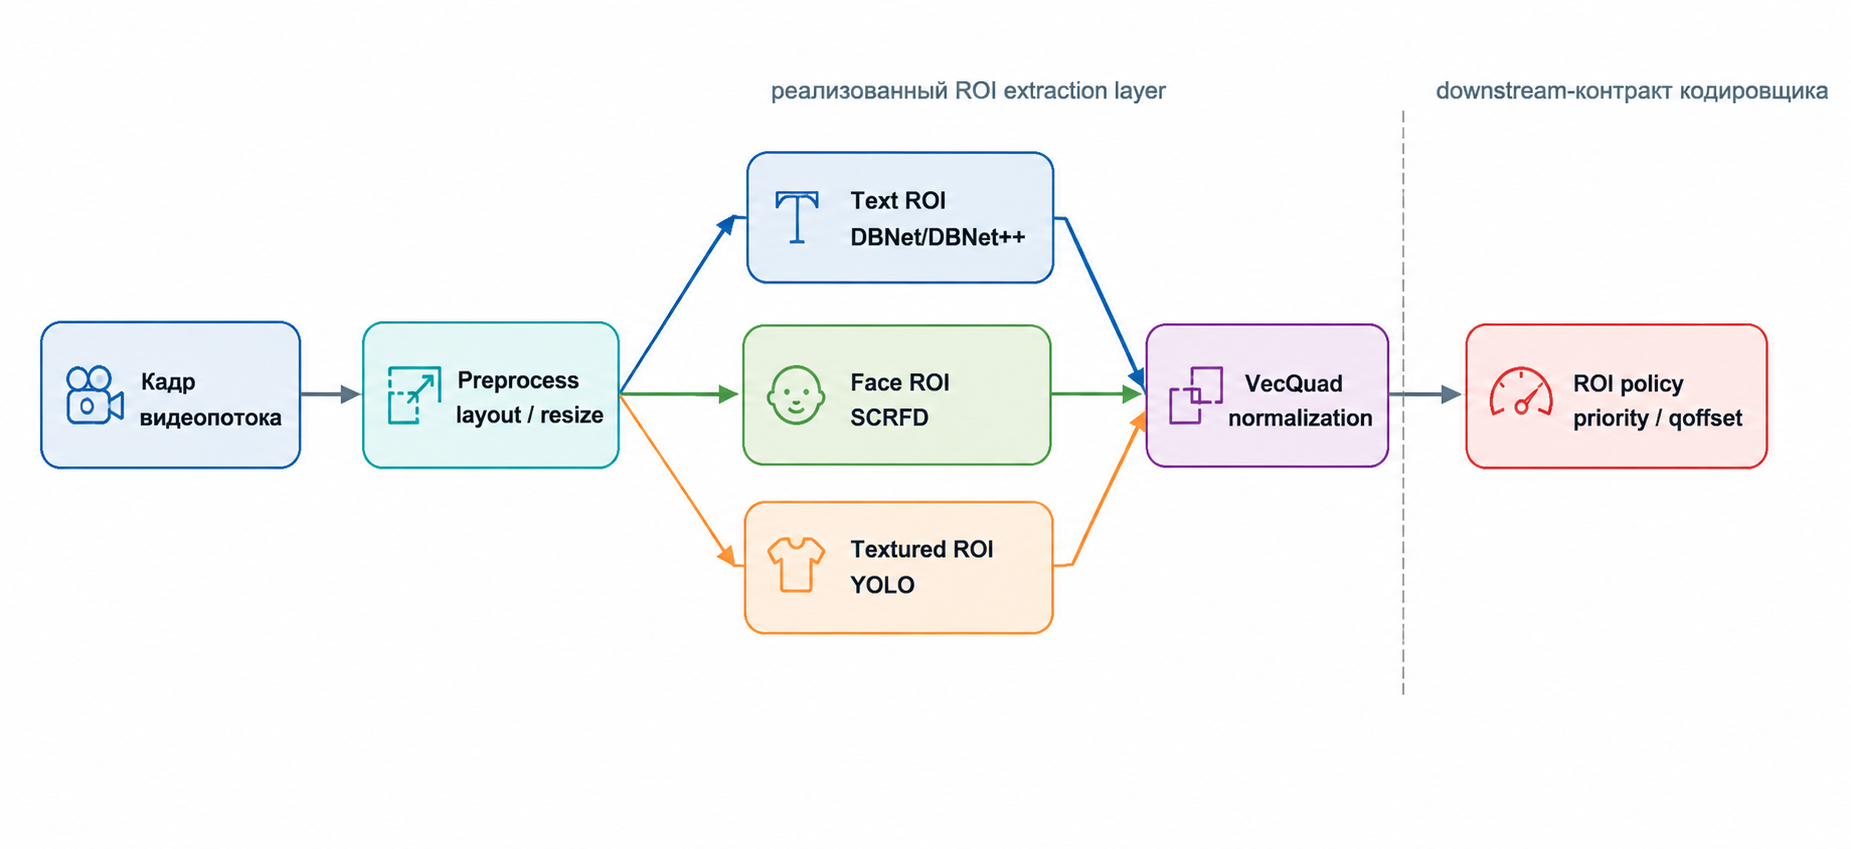
\includegraphics[width=0.96\linewidth]{architecture/roi_pipeline_overview.png}
  \caption{Архитектура ROI-aware конвейера на базе IDet: текстовые ROI, ROI лиц и текстурированные
      ROI объединяются в геометрический выход, а последующий слой преобразует его в
      приоритеты для кодировщика.}
  \label{fig:architecture}
\end{figure}

Рисунок~\ref{fig:architecture} фиксирует главное архитектурное разделение: IDet отвечает за
геометрию текста, лиц и одежды, а политика кодирования работает уже с нормализованными
областями и не зависит от внутреннего формата конкретной модели.

% 1.5 Выводы по главе

\section{Выводы по главе}

В первой главе задача облачного видеостриминга сведена к управлению ограниченными ресурсами:
битрейтом, задержкой и вычислительным бюджетом. Обычный ABR-подход выбирает качество во времени,
но не решает, какие части одного кадра важнее для зрителя.

Для этой работы ключевым является пространственное перераспределение качества. Текст, лица и
фактурные области одежды выделяются как три класса ROI, потому что их деградация заметна даже
при небольшой занимаемой площади. Дальнейшие главы поэтому рассматривают не абстрактное
улучшение всего кадра, а проверяемый путь от детекции этих областей к управляющему сигналу для
кодировщика.

% ==============================================================================
%              2. Формальная постановка задачи ROI-aware оптимизации
% ==============================================================================

\chapter{Формальная постановка задачи ROI-aware оптимизации}

% 2.1 Ограниченная оптимизация качества

\section{Ограниченная оптимизация качества}

В работе задача улучшения качества видеопотока формулируется как ограниченная оптимизация. Пусть
$B$ --- доступный битрейт, $T$ --- допустимая задержка анализа кадра, $C_{\max}$ ---
вычислительный бюджет, а $\theta$ --- параметры ROI-детектора и политики кодирования. Тогда
постановку можно записать так:
\begin{equation}
  \max_{\theta}\ \mathbb{E}\left[ Q_{\roi}(F;\theta) \right]\quad\text{при условиях}\quad
  R(F;\theta) \leq B,\quad L(F;\theta) \leq T,\quad C(F;\theta) \leq C_{\max}.
  \label{eq:constrained_opt}
\end{equation}
Здесь $R$ --- фактический расход битрейта, $L$ --- задержка обработки кадра, $C$ ---
вычислительная стоимость, а $Q_{\roi}$ --- ROI-взвешенное качество. В отличие от лабораторной
постановки, где можно максимизировать только mAP модели, в данной работе важна системная
метрика: улучшение качества должно быть достигнуто без выхода за бюджет задержки и без
чрезмерного роста вычислительной стоимости.

Эта постановка отражает практическую природу облачного видеостриминга. Даже если более тяжелая
модель точнее на валидационном разбиении, она может оказаться непригодной для конвейера
реального времени. Напротив, легкая модель с немного меньшей mAP может быть предпочтительнее,
если она обеспечивает стабильное p95/p99 и достаточное покрытие ROI.

% 2.2 Бюджет площади ROI

\section{Бюджет площади ROI}

Если защищать слишком большую часть кадра, кодировщик теряет возможность перераспределять биты.
Поэтому вводится ограничение на долю защищаемой площади:
\begin{equation}
  \frac{\left|\bigcup_{i=1}^{N} R_i\right|}{|F|} \leq \alpha,
  \label{eq:area_budget}
\end{equation}
где $\alpha$ --- максимально допустимая доля кадра, например $0.15$--$0.35$ в зависимости от
типа контента. Это ограничение важно не только математически, но и инженерно: оно защищает
систему от ложных срабатываний и от ситуации, когда ROI-aware режим фактически превращается в
кодирование всего кадра с повышенным качеством.

Бюджет площади должен применяться после объединения результатов разных детекторов. Несколько
корректных ROI по отдельности могут вместе занять слишком большую часть кадра. Особенно это
важно для текстурированных ROI: области одежды могут быть крупными, поэтому без ограничения
площади они начнут конкурировать с текстом и лицами за битовый бюджет. В типовой политике текст
имеет самый высокий приоритет, лица --- высокий, а текстурированные ROI --- средний.

% 2.3 Временная стабильность ROI

\section{Временная стабильность ROI}

Для видео важна не только точность ROI в отдельном кадре, но и стабильность во времени. Если
область резко меняет положение между соседними кадрами, это может привести к мерцанию качества
после кодирования. Для сглаживания уверенности можно использовать рекуррентную формулу:
\begin{equation}
  \hat{s}_{t} =\lambda \hat{s}_{t-1}+(1-\lambda)s_t,
  \label{eq:smoothing}
\end{equation}
где $s_t$ --- текущая уверенность детектора, $\hat{s}_t$ --- сглаженная уверенность, а $\lambda
\in [0,1]$ --- коэффициент памяти.

Дополнительно можно ввести штраф за нестабильность геометрии ROI между соседними кадрами. Для
этого используется метрика, основанная на пересечении областей:
\begin{equation}
  P_{\mathrm{flicker}} = \frac{1}{T-1} \sum_{t=2}^{T} \left(1 - \operatorname{IoU}(R_t,
  R_{t-1})\right).
  \label{eq:flicker}
\end{equation}
Здесь $R_t$ обозначает ROI на кадре $t$, а $\operatorname{IoU}(R_t, R_{t-1})$ показывает,
насколько сильно область на текущем кадре совпадает с областью на предыдущем кадре. Если две
области почти совпадают, значение IoU близко к единице, а вклад в штраф близок к нулю. Если
область резко смещается, уменьшается или появляется в другом месте кадра, IoU становится малым,
а величина $1-\operatorname{IoU}$ возрастает.

Таким образом, $P_{\mathrm{flicker}}$ можно интерпретировать как среднюю величину межкадрового
изменения ROI. Чем выше это значение, тем менее стабильна геометрия областей интереса и тем выше
риск визуального мерцания качества после передачи ROI кодировщику. Поэтому временное
сглаживание, сопровождение областей между кадрами и подавление кратковременных ложных
срабатываний должны рассматриваться как часть последующего ROI-слоя, а не как обязанность
конкретной нейросетевой модели.

% 2.4 От ROI к qoffset кодировщика

\section{От ROI к qoffset кодировщика}

FFmpeg предоставляет структуру \texttt{AVRegionOfInterest}, где область задается координатами и
параметром \texttt{qoffset}; отрицательное значение qoffset означает повышение качества
кодирования внутри ROI \cite{ffmpeg_roi}. На уровне фильтров аналогичная идея доступна через
\texttt{addroi}: фильтр прикрепляет к кадру metadata об областях интереса для последующего
кодирования, не изменяя сами пиксели \cite{ffmpeg_addroi}.

Упрощенное преобразование приоритета $p_i$ в смещение QP можно записать так:
\begin{equation}
  \Delta QP_i =-\gamma \cdot p_i \cdot (QP_{\max} - QP_{\min}),
  \label{eq:qoffset}
\end{equation}
где $p_i \in [0,1]$ --- нормированный приоритет области, а $\gamma$ --- коэффициент силы защиты.
Формула не задает конкретную реализацию кодировщика, но фиксирует общий принцип: чем важнее
область, тем сильнее отрицательное смещение QP.

% 2.5 Метрики детекции

\section{Метрики детекции}

Для модели текстурированных ROI используются стандартные метрики детекции объектов: точность,
полнота, F1, AP, mAP@0.5 и mAP@0.5:0.95 \cite{ultra_metrics}. Точность и полнота вычисляются по
формулам:
\begin{equation}
  \operatorname{Precision} =\frac{TP}{TP+FP},\qquad\operatorname{Recall} =\frac{TP}{TP+FN},
  \label{eq:precision_recall}
\end{equation}
а F1-мера определяется как
\begin{equation}
  F_1 =2
  \cdot\frac{\operatorname{Precision}\cdot\operatorname{Recall}}{\operatorname{Precision}+\operatorname{Recall}}.
  \label{eq:f1}
\end{equation}

В контексте ROI-задачи полнота особенно важна: пропуск значимой области одежды хуже, чем
неточная классификация типа одежды, потому что цель детектора текстурированных ROI --- не модная
аналитика, а защита визуально богатой области от агрессивного сжатия. Однако точность также
нельзя игнорировать: ложные текстурированные ROI увеличивают защищаемую площадь и могут отнимать
битовый бюджет у текста и лиц.

AP измеряет площадь под precision--recall кривой при заданном IoU-пороге, а mAP@0.5:0.95
усредняет AP по нескольким порогам IoU от 0.5 до 0.95. Для ROI-aware кодирования это различие
принципиально: mAP@0.5 показывает, насколько модель в целом находит объекты, а mAP@0.5:0.95
строже оценивает точность bbox. Слишком широкий bbox защищает лишний фон, а слишком узкий может
не покрыть значимую фактуру. Поэтому detection metrics должны дополняться area-based метриками
покрытия ROI.

% 2.6 Выводы по главе

\section{Выводы по главе}

Формальная постановка фиксирует главный компромисс работы: ROI-aware система должна повышать
локальное качество значимых областей, не выходя за ограничения по битрейту, задержке,
вычислительной стоимости и площади ROI. Поэтому одной mAP детектора недостаточно для вывода о
полезности системы.

Для дальнейших экспериментов это задает два уровня проверки. Первый уровень --- качество
детекции и геометрии ROI: precision, recall, AP, mAP и area-based метрики. Второй уровень ---
видеокодирование: \texttt{qoffset}, ограничение площади, стабильность ROI во времени и
ROI-взвешенные метрики качества. Только совместная проверка этих уровней позволяет сделать
аккуратный вывод о практической пользе подхода.

% ==============================================================================
%              3. Проектирование IDet и трехрежимного ROI-конвейера
% ==============================================================================

\chapter{Проектирование IDet и трехрежимного ROI-конвейера}

% 3.1 IDet как инженерное ядро работы

\section{IDet как инженерное ядро работы}

IDet --- это CPU-ориентированная C++ библиотека для детекции и нормализации областей интереса
\cite{idet}. В данной работе она рассматривается как центральный инженерный результат: задача
библиотеки состоит не в обучении единственной модели, а в связывании нескольких
специализированных детекторов с видеокодировщиком через устойчивый геометрический контракт.

Фактический публичный контракт IDet возвращает список четырехугольников \texttt{VecQuad}.
Типизация ROI, приоритеты и \texttt{qoffset} относятся к последующему слою интеграции с
кодировщиком. Такое разделение важно: IDet отвечает за компьютерное зрение и геометрию, а
адаптер кодировщика --- за конкретную политику кодирования.

Архитектурно IDet опирается на несколько принципов:
\begin{enumerate}[label=\arabic*)]
  \item критический путь обработки должен работать на CPU без зависимости от Python;
  \item модели должны быть приведены к ONNX-формату, пригодному для развертывания;
  \item инференс должен выполняться через ONNX Runtime \cite{onnx,onnxruntime};
  \item входные и выходные буферы должны переиспользоваться;
  \item число потоков должно задаваться явно;
  \item модельно-зависимые детали не должны протекать в пользовательский код.
\end{enumerate}

ONNX Runtime поддерживает оптимизацию вычислительного графа, включая слияние операций и удаление
лишних узлов \cite{ort_graph_optim}. Механизм I/O Binding позволяет заранее связать входы и
выходы с выбранными буферами, что уменьшает число копирований и делает размещение памяти более
предсказуемым \cite{ort_iobinding}.

\begin{table}[!htbp]
  \centering
  \caption{Основные модули IDet в критическом пути обработки кадра}
  \label{tab:idet_modules}
  \small
  \begin{tabularx}{\linewidth}{@{}P{0.27\linewidth}P{0.28\linewidth}Y@{}}
    \toprule
    Модуль & Ответственность & Выходной результат \\
    \midrule
    Слой входного кадра &
    Прием кадра, проверка формата, масштабирование и подготовка рабочего представления. &
    Нормализованный кадр или набор плиток. \\
    Слой предобработки &
    Letterbox, изменение размера, нормализация каналов, преобразование раскладки и заполнение
      входных тензорных буферов. &
    Готовые входные буферы для ONNX Runtime. \\
    Адаптеры моделей &
    Обертки над детекторами текста, лиц и текстур; скрывают формат выходов конкретной модели. &
    Сырые кандидаты: область, оценка уверенности, класс или тип. \\
    Слой постобработки &
    Пороговая фильтрация, декодирование координат, NMS, сшивание плиток и обратное
      преобразование координат. &
    Кандидаты ROI в координатах исходного кадра. \\
    Публичный геометрический слой &
    Приведение результата к публичному контракту библиотеки. &
    \texttt{VecQuad}. \\
    \bottomrule
  \end{tabularx}
\end{table}

\begin{table}[!htbp]
  \centering
  \caption{Последующие слои интеграции IDet с видеокодировщиком}
  \label{tab:idet_integration_modules}
  \small
  \begin{tabularx}{\linewidth}{@{}P{0.27\linewidth}P{0.28\linewidth}Y@{}}
    \toprule
    Слой & Ответственность & Выходной результат \\
    \midrule
    Последующий ROI-слой &
    Добавление типа ROI, уверенности, приоритета, ограничения площади и временного сглаживания
      поверх геометрии. &
    Метаданные ROI для кодировщика. \\
    Адаптер кодировщика &
    Преобразование метаданных ROI в \texttt{qoffset}, ROI side data или резервную политику. &
    Управляющая информация для кодировщика. \\
    Слой измерений &
    Измерение задержки, числа ROI, площади ROI и стабильности результатов. &
    p50/p95/p99 и диагностические отчеты. \\
    \bottomrule
  \end{tabularx}
\end{table}

\begin{figure}[!htbp]
  \centering
  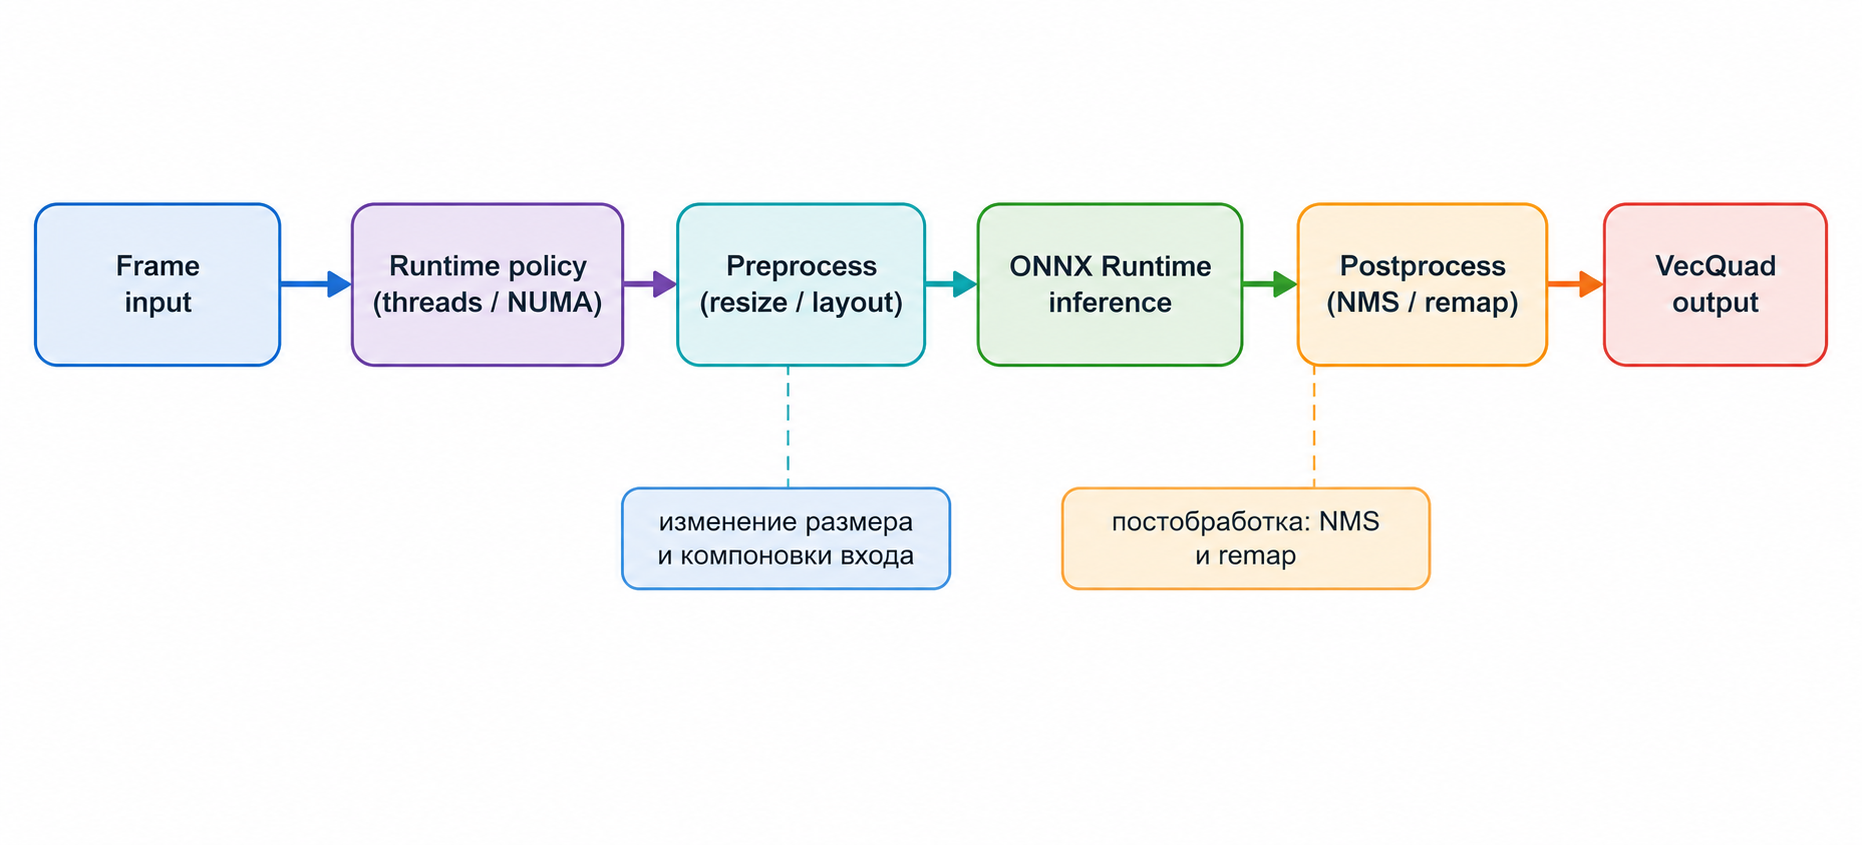
\includegraphics[width=0.96\linewidth]{architecture/idet_frame_runtime_path.png}
  \caption{Путь обработки одного кадра в IDet: подготовка изображения, CPU-инференс, постобработка
      и возврат списка \texttt{VecQuad}.}
  \label{fig:idet_runtime}
\end{figure}

Рисунок~\ref{fig:idet_runtime} показывает, что на критическом пути нет обучающего
Python-конвейера: кадр проходит через подготовку входа, ONNX Runtime и модельно-зависимую
постобработку, после чего внешний слой получает только унифицированную геометрию.

% 3.2 Жизненный цикл обработки кадра

\section{Жизненный цикл обработки кадра}

Жизненный цикл кадра в IDet начинается до запуска нейросетевой модели. Сначала система получает
кадр в исходном разрешении, проверяет формат пикселей и выбирает режим обработки: полный кадр,
tiled inference, downscale или повторное использование ROI с предыдущих кадров. Затем
выполняется предобработка: resize/letterbox, нормализация и преобразование layout в формат,
ожидаемый ONNX-моделью.

После инференса каждый движок декодирует выходы своей модели. Движок текста преобразует карты
вероятностей DBNet-подобной модели в четырехугольники, движок лиц декодирует выходы SCRFD, а
движок текстур преобразует выходы YOLO в кандидаты \texttt{bbox}/\texttt{quad}. На публичном
уровне результат нормализуется в \texttt{VecQuad}; последующий слой уже поверх этой геометрии
добавляет тип, приоритет и \texttt{qoffset}-рекомендацию.

\begin{table}[!htbp]
  \centering
  \caption{Жизненный цикл кадра в ROI-aware конвейере на базе IDet}
  \label{tab:frame_lifecycle}
  \small
  \begin{tabularx}{\linewidth}{@{}P{0.08\linewidth}P{0.26\linewidth}Y@{}}
    \toprule
    Шаг & Этап & Смысл этапа \\
    \midrule
    1 &
    Получение кадра &
    Получение кадра и фиксация размеров, временной метки и формата пикселей. \\
    2 &
    План обработки &
    Выбор режима обработки: полный кадр, плитки, пропуск тяжелого детектора или перенос ROI. \\
    3 &
    Предобработка &
    Подготовка входных буферов: изменение размера, letterbox, нормализация, преобразование
      раскладки. \\
    4 &
    Инференс &
    Выполнение одной или нескольких сессий ONNX Runtime с контролируемым числом потоков. \\
    5 &
    Постобработка модели &
    Декодирование выходов моделей, пороговая фильтрация, NMS, сшивание плиток и обратное
      отображение координат. \\
    6 &
    Публичный геометрический выход &
    Возврат унифицированной геометрии в формате \texttt{VecQuad}. \\
    7 &
    Интеграция ROI &
    Добавление типа ROI, сортировка, слияние пересечений, ограничение площади и временное
      сглаживание. \\
    8 &
    Управление кодировщиком &
    Преобразование метаданных ROI в \texttt{qoffset}, side data или резервные параметры. \\
    9 & Телеметрия & Запись задержки, числа ROI, площади ROI и диагностической информации. \\
    \bottomrule
  \end{tabularx}
\end{table}

% 3.3 Ответственность адаптеров детекторов

\section{Ответственность адаптеров детекторов}

Адаптер в IDet отвечает за преобразование конкретной модели в общий контракт библиотеки. Он не
должен принимать решения о том, какие ROI важнее для кодировщика: это задача последующего
ROI-слоя. Такой принцип уменьшает связность и позволяет заменять модели без переписывания слоя
интеграции с кодировщиком.

\begin{table}[!htbp]
  \centering
  \caption{Ответственность адаптеров IDet}
  \label{tab:adapter_responsibilities}
  \small
  \begin{tabularx}{\linewidth}{@{}P{0.23\linewidth}P{0.30\linewidth}Y@{}}
    \toprule
    Адаптер & Внутренняя ответственность & Что не входит в ответственность \\
    \midrule
    Адаптер текста &
    Предобработка под DBNet/DBNet++, декодирование карт текста, извлечение многоугольников,
      фильтрация по уверенности. &
    Глобальный приоритет текста относительно лица и текстурированных ROI. \\
    Адаптер лиц &
    Изменение размера и нормализация под SCRFD, декодирование кандидатов, NMS лиц, нормализация
      уверенности. &
    Решение о \texttt{qoffset} и ограничение общей площади ROI. \\
    Адаптер текстур &
    Предобработка под YOLO, декодирование координат и классов, NMS, обратное отображение
      координат из letterbox-пространства. &
    Интерпретация классов одежды как политик кодирования. \\
    Адаптер кодировщика &
    Преобразование метаданных ROI в FFmpeg ROI side data, карту \texttt{qoffset} или резервные
      параметры. &
    Запуск детекторов и изменение выходов моделей. \\
    \bottomrule
  \end{tabularx}
\end{table}

% 3.4 Реальный публичный контракт IDet

\section{Реальный публичный контракт IDet}

Важное архитектурное решение IDet состоит в том, что конкретная модель не протекает в
пользовательский код. Публичный слой выбирает задачу и движок через \texttt{Task} и
\texttt{EngineKind}, а пользователь получает геометрию областей как \texttt{VecQuad}. Ниже
приведен сокращенный фрагмент публичного интерфейса библиотеки.

\begin{lstlisting}[
    caption={Сокращенный фрагмент публичного API IDet},
    label={lst:idet_public_api}
  ]
namespace idet {

enum class Task : std::uint8_t {
    None = 0,
    Text,
    Face,
    Cloth,
};

enum class EngineKind : std::uint8_t {
    None = 0,
    DBNet,
    SCRFD,
    Yolo,
};

struct Point2f {
    float x = 0.0f;
    float y = 0.0f;
};

using Quad = std::array<Point2f, 4>;
using VecQuad = std::vector<Quad>;

struct GridSpec {
    int rows = 1;
    int cols = 1;
};

struct InferenceOptions {
    bool bind_io = false;

    float bin_thresh = 0.3f;
    float box_thresh = 0.5f;
    float nms_iou = 0.3f;

    int min_roi_size_w = 5;
    int min_roi_size_h = 5;

    GridSpec fixed_input_dim{0, 0};
    GridSpec tiles_dim{1, 1};
    float tile_overlap = 0.1f;
};

struct RuntimePolicy {
    int ort_intra_threads = 1;
    int ort_inter_threads = 1;
    int tile_omp_threads = 1;

    bool soft_mem_bind = true;
    bool suppress_opencv = true;
};

struct DetectorConfig final {
    Task task = Task::None;
    EngineKind engine = EngineKind::None;

    InferenceOptions infer{};
    RuntimePolicy runtime{};

    std::string model_path{};
    bool verbose = true;

    [[nodiscard]] Status validate() const noexcept;

    static DetectorConfig setup(Task task, std::string model_path);
};

class Detector final {
public:
    Detector() noexcept = default;
    ~Detector() noexcept;

    Detector(Detector&& other) noexcept;
    Detector& operator=(Detector&& other) noexcept;

    Detector(const Detector&) = delete;
    Detector& operator=(const Detector&) = delete;

    explicit operator bool() const noexcept;

    Task task() const noexcept;
    EngineKind engine() const noexcept;

    void reset() noexcept;

    static Result<Detector> create(
        const DetectorConfig& config
    ) noexcept;

    Status prepare_binding(
        int width,
        int height,
        int contexts
    ) noexcept;

    Result<VecQuad> detect(
        const Image& image
    ) noexcept;

    Result<VecQuad> detect_bound(
        const Image& image,
        int ctx_idx
    ) noexcept;

private:
    void* impl_ = nullptr;
    const detail::DetectorVTable* vtbl_ = nullptr;
};

} // namespace idet
\end{lstlisting}

Этот контракт фиксирует фактическую границу между C++ библиотекой и внешним видеоконвейером.
Модельно-зависимые детали --- letterbox, преобразование раскладки, нормализация входа,
декодирование выходов, пороговая фильтрация и NMS --- скрыты внутри движков. Последующий слой,
необходимый для ROI-aware кодирования, должен добавлять к возвращенной геометрии тип области,
приоритет и \texttt{qoffset}; в текущем публичном API это не отдельный класс библиотеки.

% 3.5 Последующий контракт метаданных ROI

\section{Последующий контракт метаданных ROI}

Для кодировщика одной геометрии недостаточно. Ему важно знать тип области, уверенность,
приоритет и рекомендуемую силу защиты. Поэтому поверх \texttt{VecQuad} вводится последующая
запись метаданных ROI. Она может быть реализована в слое интеграции с кодировщиком и не должна
смешиваться с текущим публичным API IDet.

\begin{table}[!htbp]
  \centering
  \caption{Последующий контракт метаданных ROI между детекторами, ROI-слоем и адаптером
      кодировщика}
  \label{tab:richroi_contract}
  \small
  \begin{tabularx}{\linewidth}{@{}P{0.24\linewidth}P{0.24\linewidth}Y@{}}
    \toprule
    Поле & Пример & Назначение \\
    \midrule
    \texttt{kind} &
    \texttt{text}, \texttt{face}, \texttt{texture} &
    Тип ROI, определяющий приоритет и политику \texttt{qoffset}. \\
    \texttt{quad/bbox} &
    \texttt{TL,TR,BR,BL} или \texttt{x1,y1,x2,y2} &
    Геометрия области в координатах исходного кадра. \\
    \texttt{confidence} & $0.0$--$1.0$ & Уверенность конкретного детектора. \\
    \texttt{priority} & $0.0$--$1.0$ & Системный приоритет после учета типа и уверенности. \\
    \texttt{area} &
    доля кадра &
    Используется для бюджета площади и отсечения чрезмерно больших ROI. \\
    \texttt{qoffsetHint} &
    отрицательное значение &
    Предлагаемое смещение квантования для адаптера кодировщика. \\
    \texttt{source} &
    \texttt{dbnet}, \texttt{scrfd}, \texttt{yolo26n} &
    Источник ROI для диагностики и ablation study. \\
    \texttt{trackId} &
    целое число или \texttt{none} &
    Связь ROI между кадрами для временного сглаживания. \\
    \bottomrule
  \end{tabularx}
\end{table}

% 3.6 Приоритеты и разрешение конфликтов

\section{Приоритеты и разрешение конфликтов}

В системе вводится иерархия приоритетов: текст $>$ лицо $>$ текстурированные ROI $>$ фон. Текст
получает максимальный приоритет, потому что даже небольшие артефакты могут сделать его
нечитаемым. Лицо получает высокий приоритет из-за чувствительности пользователя к искажениям
человеческой внешности. Текстурированные ROI получают средний приоритет: фактура повышает
воспринимаемую резкость, но не должна вытеснять текст и лица при ограниченном бюджете площади.

\begin{table}[!htbp]
  \centering
  \caption{Алгоритм слияния ROI}
  \label{tab:roi_fusion_algorithm}
  \begin{tabularx}{\linewidth}{@{}P{0.08\linewidth}Y@{}}
    \toprule
    Шаг & Действие \\
    \midrule
    1 & Получить кандидаты ROI от адаптеров текста, лиц и текстур. \\
    2 & Нормировать координаты, уверенность и тип области к последующей записи метаданных ROI. \\
    3 & Удалить кандидаты с уверенностью ниже порога, зависящего от типа ROI. \\
    4 & Отсортировать ROI по приоритету: текст $>$ лицо $>$ текстура $>$ фон. \\
    5 & Объединить сильно пересекающиеся области с учетом IoU и типа области. \\
    6 & Ограничить суммарную защищаемую площадь кадра заданным бюджетом площади. \\
    7 & Применить временное сглаживание к координатам и уверенности для уменьшения мерцания ROI. \\
    8 & Вернуть упорядоченный список метаданных ROI для адаптера кодировщика. \\
    \bottomrule
  \end{tabularx}
\end{table}

% 3.7 Память, буферы и критический путь без динамических аллокаций

\section{Память, буферы и критический путь без динамических аллокаций}

Для видеостриминга в реальном времени важна не только средняя задержка, но и устойчивость
p95/p99. Динамические аллокации в критическом пути приводят к джиттеру: отдельные кадры внезапно
обрабатываются дольше из-за выделения памяти, освобождения памяти или переразмещения
контейнеров. Поэтому IDet должен использовать явную модель владения буферами.

\begin{table}[!htbp]
  \centering
  \caption{Модель владения буферами в IDet}
  \label{tab:buffer_ownership}
  \small
  \begin{tabularx}{\linewidth}{@{}P{0.24\linewidth}P{0.24\linewidth}Y@{}}
    \toprule
    Буфер & Владелец & Правило использования \\
    \midrule
    Исходный кадр &
    Слой входного кадра &
    Только чтение после получения кадра; исходное изображение не меняется детекторами. \\
    Предобработанный вход &
    Слой предобработки &
    Переиспользуется между кадрами одного размера; заполняется перед инференсом. \\
    Входные/выходные тензоры ONNX &
    Бэкенд инференса &
    Выделяются при инициализации сессии или при смене формы входа. \\
    Массивы кандидатов &
    Адаптер модели &
    Очищаются и переиспользуются; вместимость растет только вне критического пути. \\
    Рабочий буфер NMS &
    Слой постобработки &
    Общий временный буфер для сортировки и подавления кандидатов. \\
    \texttt{VecQuad} &
    Публичный геометрический слой &
    Финальный геометрический результат публичного API. \\
    Список метаданных ROI &
    Последующий ROI-слой &
    Список областей с типом и приоритетом для адаптера кодировщика. \\
    \bottomrule
  \end{tabularx}
\end{table}

% 3.8 Политика потоков

\section{Политика потоков}

IDet должен контролировать два уровня параллелизма: внешний уровень обработки кадров/плиток и
внутренний уровень потоков ONNX Runtime. Если оба уровня включены без ограничений, возникает
переподписка потоков: несколько пулов потоков конкурируют за одни и те же CPU-ядра, что ухудшает
p95/p99 задержку. Поэтому политика потоков должна задаваться явно и быть частью конфигурации.

\begin{table}[!htbp]
  \centering
  \caption{Политика потоков в IDet}
  \label{tab:threading_policy}
  \small
  \begin{tabularx}{\linewidth}{@{}P{0.23\linewidth}P{0.27\linewidth}Y@{}}
    \toprule
    Уровень & Настраиваемый параметр & Инженерный смысл \\
    \midrule
    Параллелизм кадров &
    Число одновременно обрабатываемых кадров. &
    Увеличивает пропускную способность, но может ухудшить задержку отдельного кадра. \\
    Параллелизм плиток &
    Число плиток, обрабатываемых параллельно. &
    Полезно для крупных кадров, но требует аккуратного сшивания результатов. \\
    Потоки ORT intra-op &
    Число потоков внутри оператора ONNX Runtime. &
    Влияет на скорость сверточных и матричных операций. \\
    Потоки ORT inter-op &
    Параллелизм между независимыми узлами графа. &
    Эффективен не для всех моделей; требует профилирования. \\
    Частота запуска детектора &
    Частота запуска каждой ветки ROI. &
    Позволяет запускать тяжелые детекторы реже и переносить ROI во времени. \\
    \bottomrule
  \end{tabularx}
\end{table}

% 3.9 Инварианты и отказоустойчивость

\section{Инварианты и отказоустойчивость}

Для производственного конвейера важно определить не только идеальный путь, но и инварианты,
которые должны сохраняться при ошибках. IDet и последующий ROI-слой должны гарантировать
следующие свойства:
\begin{enumerate}[label=\arabic*)]
  \item координаты ROI находятся внутри границ исходного кадра;
  \item суммарная площадь защищаемых областей не превышает заданный бюджет $\alpha$;
  \item пересекающиеся ROI не приводят к конфликтующим qoffset одного и того же блока;
  \item при сбое одного детектора остальные режимы могут продолжить работу;
  \item при превышении бюджета задержки система может временно перейти к переносу ROI предыдущих
      кадров или к более дешевой ветке;
  \item отсутствие нативной поддержки ROI в кодировщике не должно ломать кодирование: адаптер
      кодировщика обязан перейти к резервной политике.
\end{enumerate}

Эти инварианты показывают, что IDet проектируется не как демонстрационный скрипт, а как слой,
который может быть встроен в реальный видеоконвейер с ограничениями по времени, памяти и
надежности.

% 3.10 Выводы по главе

\section{Выводы по главе}

IDet в работе выступает не как одиночная модель, а как C++ слой, который приводит разные
детекторы к одному геометрическому контракту. Публичный выход \texttt{VecQuad} намеренно
минимален: он скрывает DBNet-, SCRFD- и YOLO-специфику и позволяет внешнему видеоконвейеру
работать с единым представлением областей.

Последующие метаданные ROI, приоритеты и \texttt{qoffset} отделены от публичного API
библиотеки. Такое разделение делает архитектуру последовательной: IDet отвечает за CPU-инференс,
буферы, потоки, tiled inference и геометрию, а адаптер кодировщика отвечает за конкретную
политику качества в H.264/HEVC/FFmpeg или другом backend.

% ==============================================================================
%          4. Детектор текстурированных ROI: данные, обучение и экспорт
% ==============================================================================

\chapter{Детектор текстурированных ROI: данные, обучение и экспорт}

% 4.1 Мотивация детекции текстурированных ROI

\section{Мотивация детекции текстурированных ROI}

ROI-aware видеокодирование часто связывают с лицами и текстом, поскольку эти области имеют
очевидную семантическую ценность. Однако в пользовательском видео существенную часть ощущения
резкости формируют текстуры: одежда ведущего, ткань, узор, ворс и другие мелкие регулярные
структуры. При сильном сжатии такие области теряют высокочастотные детали и превращаются в
сглаженные пятна. Поэтому текстурированные ROI рассматриваются как третий режим IDet: он не
конкурирует с текстовыми ROI и ROI лиц, а расширяет систему на визуально богатые области.

Для этой ветки используется объектный детектор семейства YOLO, обученный на согласованной
таксономии одежды. Выбор детекции объектов вместо общей модели визуальной значимости связан с
инженерной управляемостью: \texttt{bbox} легко преобразовать в ROI кодировщика, ошибки можно
анализировать через AP и матрицу ошибок, а задержку можно профилировать в CPU-ориентированном
контуре.

% 4.2 Конвейер обучения YOLO

\section{Конвейер обучения YOLO}

Для обучения детектора текстурированных ROI используется отдельный воспроизводимый конвейер
обучения YOLO \cite{pipeline}. Его задача --- обеспечить полный цикл подготовки и проверки
модели: перевод исходных аннотаций в YOLO-представление, согласование таксономии, аудит
разметки, запуск обучения, построение отчетов, экспорт ONNX и последующую проверку,
ориентированную на среду выполнения. Это отличает конвейер от разового обучающего скрипта:
модель не считается готовой после появления контрольной точки, пока не проверены данные,
метрики, переносимость ONNX-графа и контракт развертывания.

Конвейер разделяет доменную логику и CLI-слой. Датасетная часть отвечает за конвертацию исходных
схем, статистический аудит и подготовку YAML-описания данных. Обучающая часть строит план
обучения и запускает Ultralytics YOLO. Отчетная часть формирует поклассовые AP и анализ матриц
ошибок. ONNX-часть выполняет экспорт, проверку графа, оптимизацию и подготовку артефактов под
CPU-среду выполнения. Поддержка ONNX-экспорта важна, поскольку Ultralytics рассматривает режим
экспорта как основной путь переноса обученной модели в форматы развертывания, включая ONNX
\cite{ultra_export,ultra_onnx}.

\begin{figure}[!htbp]
  \centering
  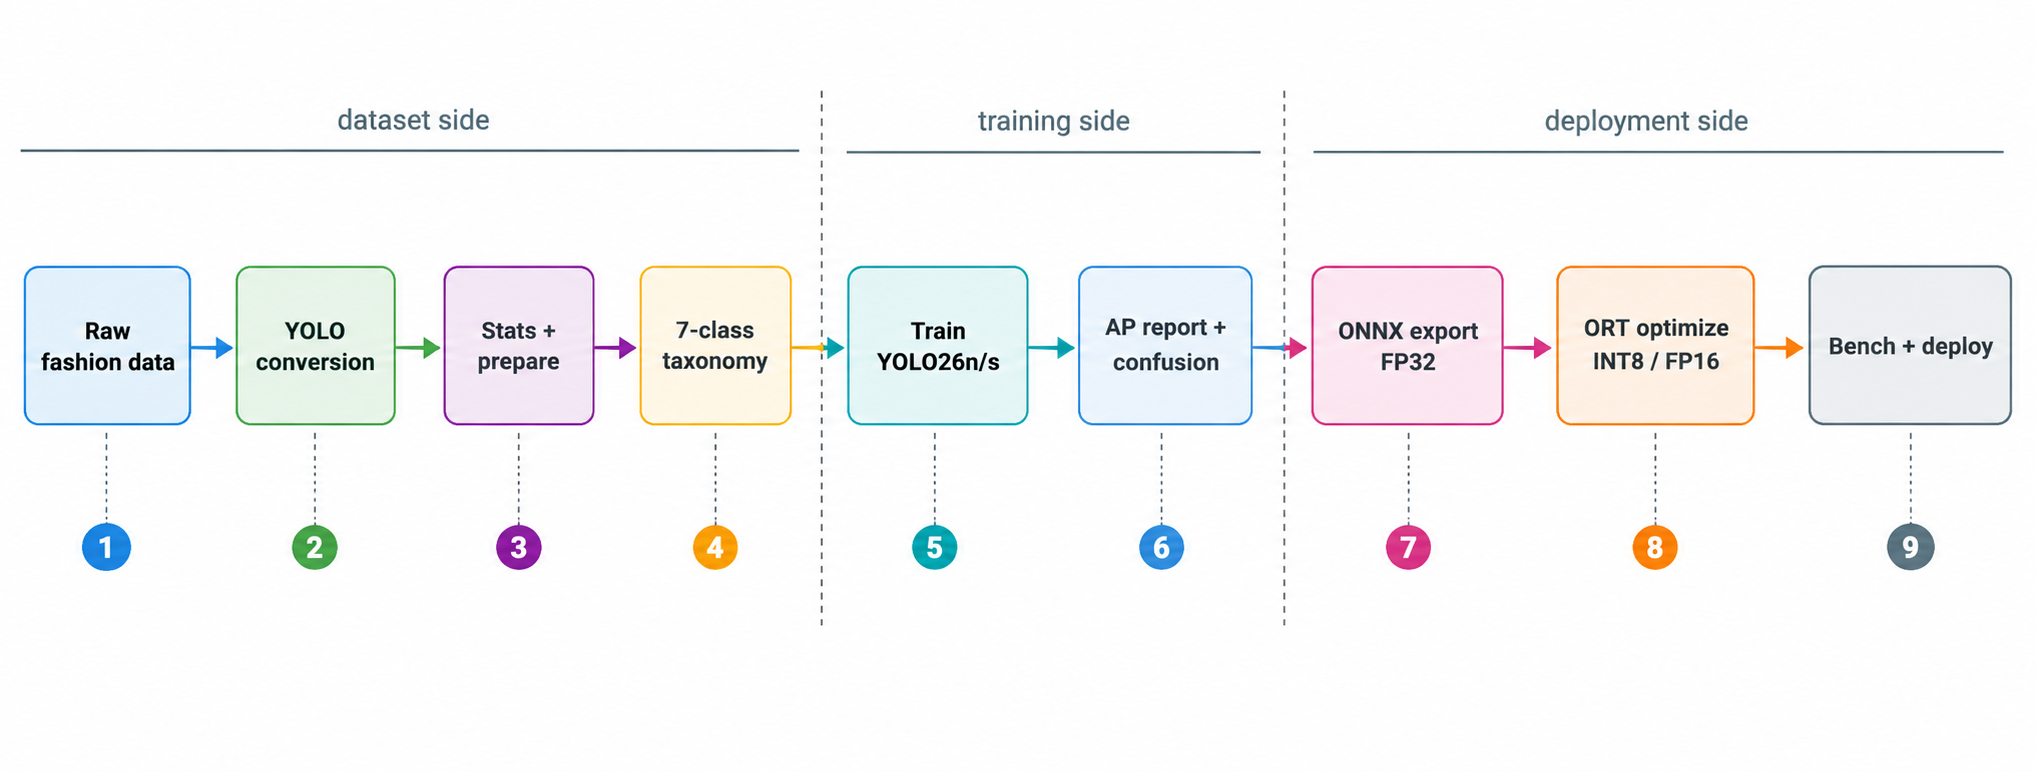
\includegraphics[width=0.96\linewidth]{yolo/yolo_training_pipeline.png}
  \caption{Конвейер обучения YOLO для детектора текстурированных ROI: конвертация и аудит
      датасетов, обучение, анализ AP и матриц ошибок, экспорт в ONNX, оптимизация среды
      выполнения и проверка артефакта для развертывания.}
  \label{fig:generic_pipeline}
\end{figure}

Рисунок~\ref{fig:generic_pipeline} важен для границы ответственности: подготовка данных,
обучение и deployment-ветка отделены друг от друга. ONNX-артефакт появляется только после
проверки обученной модели, поэтому он не подменяет валидационные отчеты и не смешивается с
исходными \texttt{runs/}.

Конвейер обучения не является частью критического пути IDet и не исполняется при обработке
кадра. Его результат --- проверенный набор обучающих данных, отчетов и артефактов для
развертывания, которые затем передаются в контур C++/ONNX Runtime. Благодаря этому IDet остается
CPU-ориентированной библиотекой без зависимости от Python-фреймворка обучения.

% 4.3 Исходные датасеты и единая таксономия

\section{Исходные датасеты и единая таксономия}

Использовались два исходных датасета: DeepFashion2 и Fashionpedia. DeepFashion2 содержит
изображения одежды с аннотациями для detection, segmentation, landmarks и retrieval
\cite{deepfashion2}. Fashionpedia построена вокруг fashion ontology и содержит категории одежды,
части одежды и fine-grained attributes \cite{fashionpedia}. Оба датасета были переведены в
YOLO-формат, после чего исходные категории были приведены к общей 7-классовой таксономии.

Целевая таксономия включает классы:
\begin{enumerate}[label=\arabic*)]
  \item \texttt{top\_sleeved};
  \item \texttt{outerwear};
  \item \texttt{top\_sleeveless};
  \item \texttt{shorts};
  \item \texttt{trousers};
  \item \texttt{skirt};
  \item \texttt{dress}.
\end{enumerate}

Смысл этой таксономии не в сохранении полной семантической детализации fashion-датасетов. Для
кодировщика важнее другой вопрос: есть ли в области визуально значимая фактура, которую
нежелательно разрушать агрессивным квантованием. Поэтому близкие категории объединяются до
уровня, достаточного для ROI-политики. Это снижает несовместимость DeepFashion2 и Fashionpedia,
уменьшает число редких классов и делает выход модели стабильнее для последующего решения о
приоритете.

% 4.4 Аудит датасетов после конвертации

\section{Аудит датасетов после конвертации}

В таблице~\ref{tab:dataset_overview} приведена сводка по трем конфигурациям: DeepFashion2,
Fashionpedia и объединенному набору. Во всех случаях отсутствуют пустые разметочные записи,
отсутствующие метки, «осиротевшие» метки и нечитаемые изображения. Это важно: качество модели
начинается не с архитектуры, а с корректности подготовленного корпуса.

\begin{table}[!htbp]
  \centering
  \caption{Сводная статистика датасетов после конвертации в YOLO-формат}
  \label{tab:dataset_overview}
  \small
  \begin{tabularx}{\linewidth}{@{}Y Z Z Z Z Z@{}}
    \toprule
    Датасет & Images & Instances & Train img & Val img & Test img \\
    \midrule
    DeepFashion2 & 224114 & 364675 & 179291 & 22411 & 22412 \\
    Fashionpedia & 45445 & 74724 & 36356 & 4544 & 4545 \\
    DF2+FP & 269559 & 439399 & 234516 & 32347 & 2696 \\
    \bottomrule
  \end{tabularx}
\end{table}

Аудит выполняет две функции. Во-первых, он подтверждает воспроизводимость training pipeline:
каждый split содержит изображения, разметку и активные классы. Во-вторых, он задает границы
интерпретации результатов. Если после конвертации меняются пропорции train/val/test или исчезает
часть объектов, итоговая mAP уже не отражает качество исходного корпуса. Поэтому до обучения
важно проверять не только количество изображений, но и число instances, распределение классов,
геометрию bbox и наличие некорректных строк разметки.

\begin{figure}[!htbp]
  \centering
  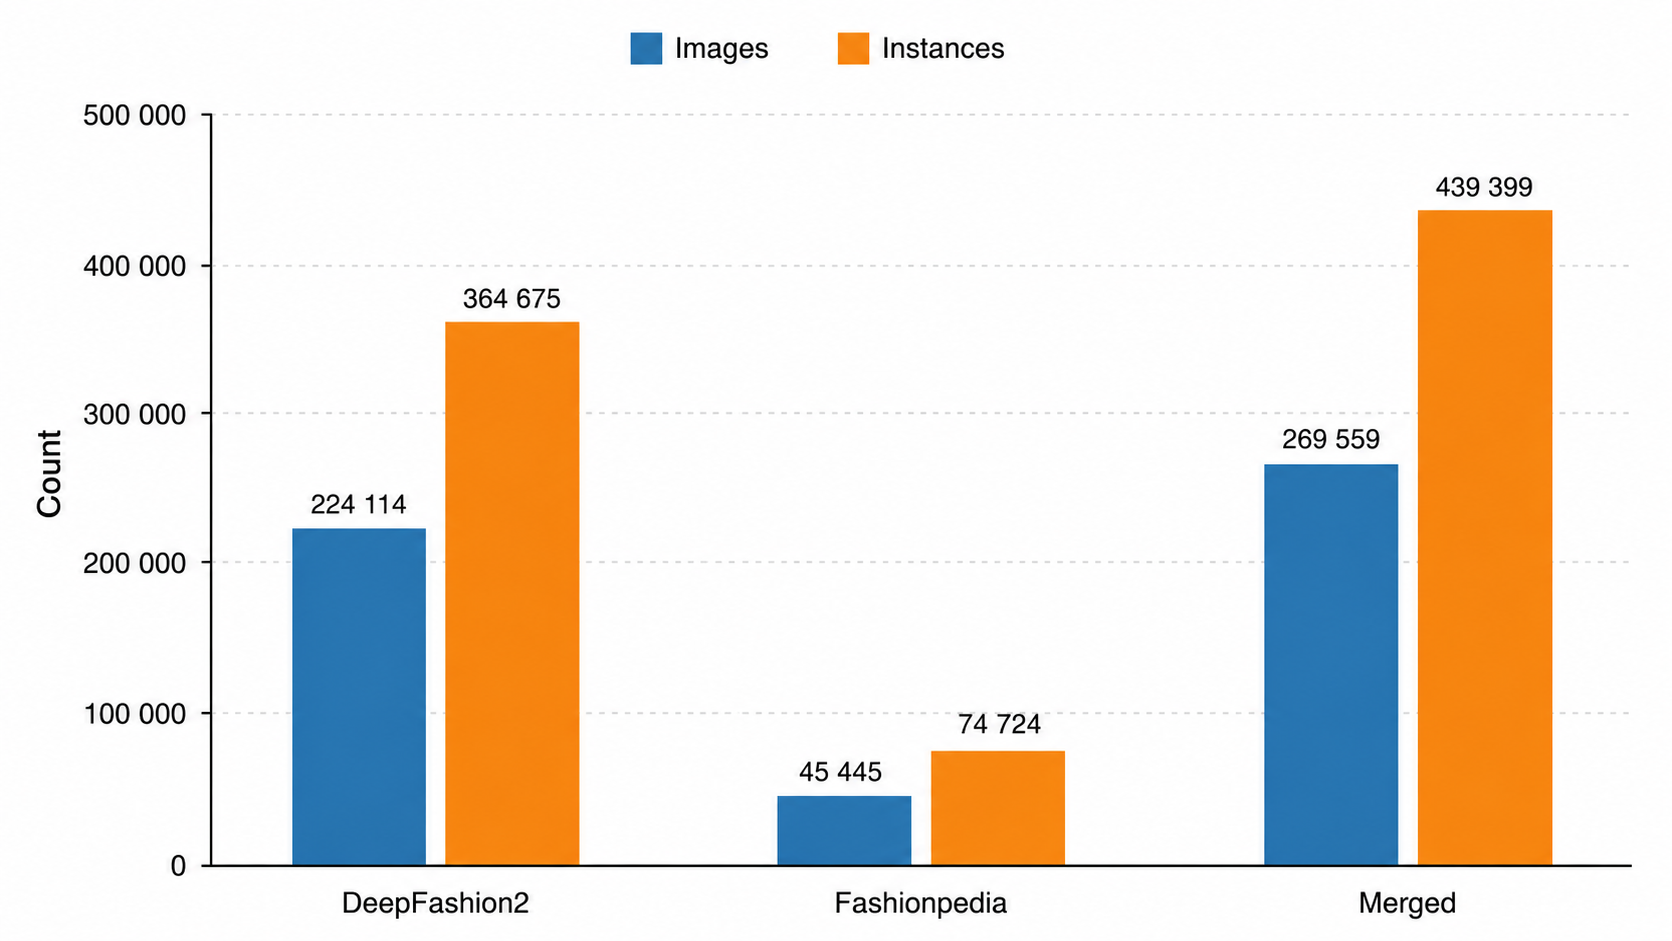
\includegraphics[width=0.86\linewidth]{datasets/dataset_image_counts.png}
  \caption{Сравнение масштаба датасетов после приведения к общей таксономии.}
  \label{fig:dataset_scale}
\end{figure}

Рисунок~\ref{fig:dataset_scale} показывает практический смысл объединения датасетов: корпус
растет с 224114 до 269559 изображений и с 364675 до 439399 объектов. Для обучения textured ROI
важен не только прирост размера, но и большее разнообразие примеров одежды.

\begin{figure}[!htbp]
  \centering
  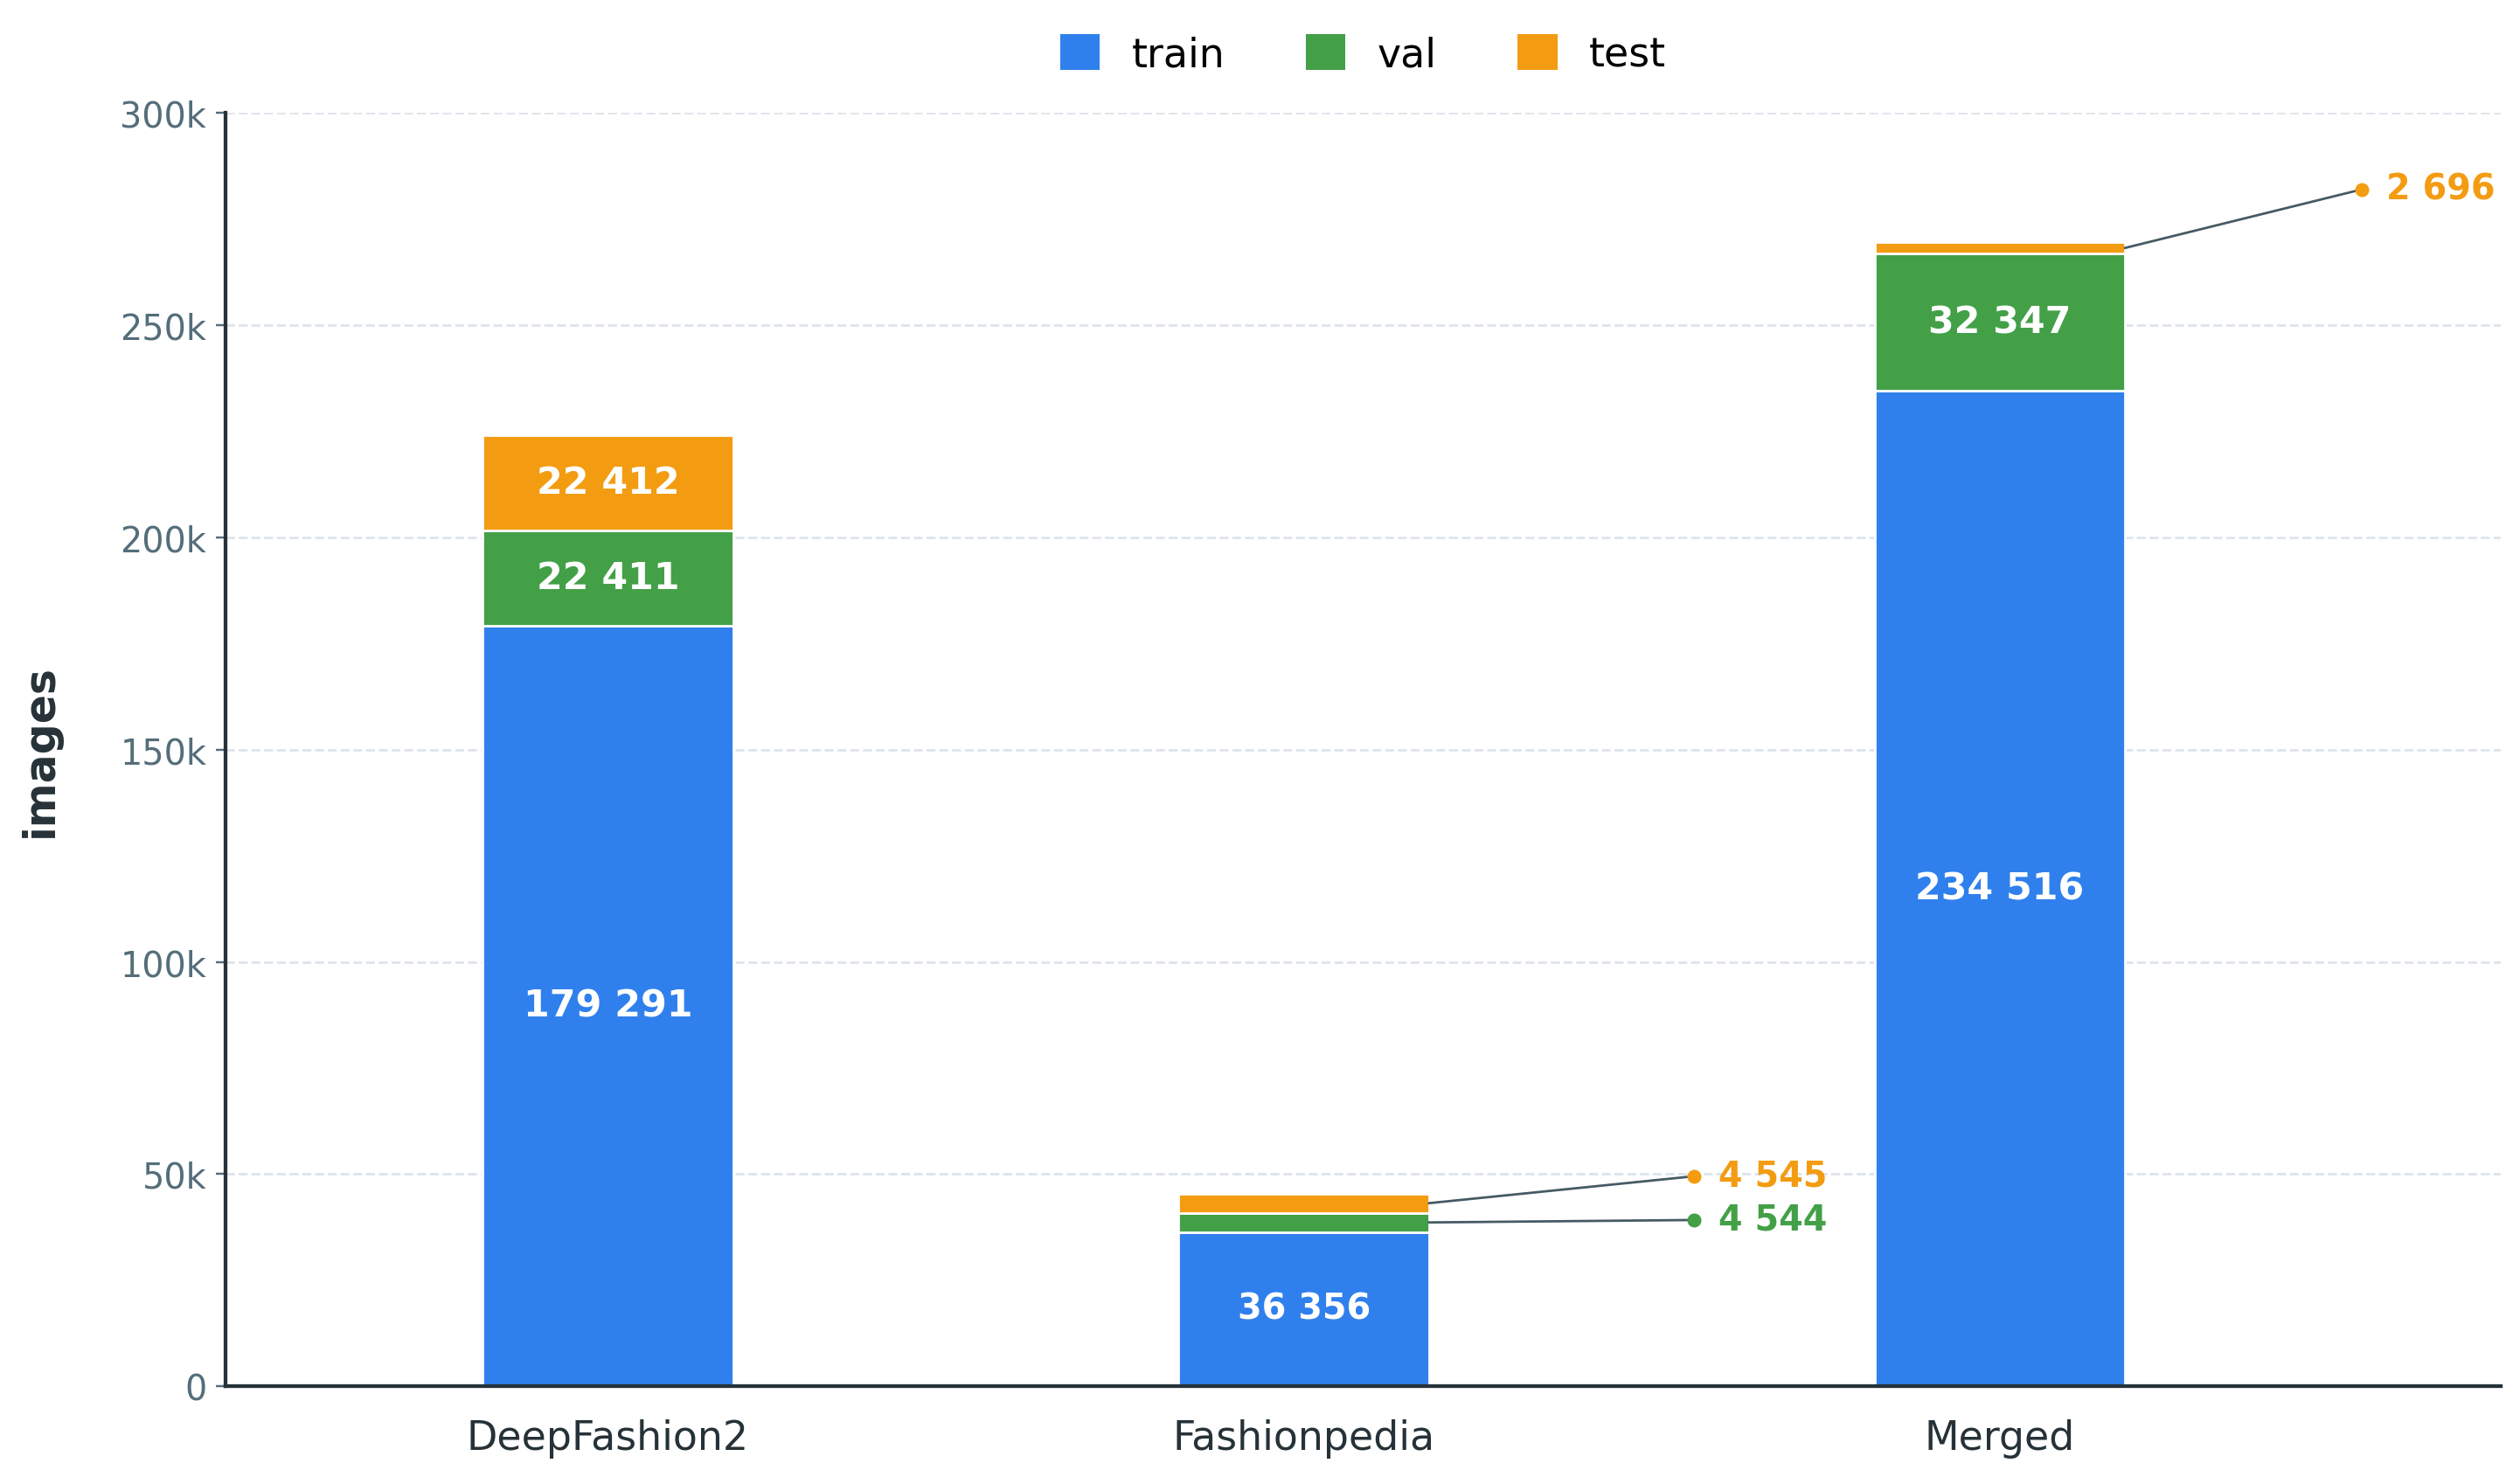
\includegraphics[width=0.86\linewidth]{datasets/dataset_split_distribution.png}
  \caption{Распределение изображений по train/val/test-разбиениям для DeepFashion2, Fashionpedia и
      объединенного набора.}
  \label{fig:split_distribution}
\end{figure}

На рисунке~\ref{fig:split_distribution} видно, что train-разбиение доминирует во всех
вариантах, а у объединенного набора test-часть существенно меньше train/val. Поэтому итоговые
выводы по модели нужно читать вместе с указанием конкретного split, на котором считались
метрики.

% 4.5 Дисбаланс классов

\section{Дисбаланс классов}

Класс \texttt{top\_sleeved} доминирует во всех конфигурациях. В DeepFashion2 он составляет
126230 объектов, в Fashionpedia --- 24803, а в объединенном наборе --- 151033. При этом в
Fashionpedia класс \texttt{top\_sleeveless} содержит только 741 объект, что создает сильный
imbalance. После объединения редкие классы получают больше примеров, а отношение крупнейшего
класса к минимальному становится мягче.

\begin{table}[!htbp]
  \centering
  \caption{Распределение объектов по классам в объединенном датасете}
  \label{tab:merged_classes}
  \small
  \begin{tabularx}{\linewidth}{@{}P{0.28\linewidth} Z Z Z Z@{}}
    \toprule
    Класс & Train & Val & Test & Total \\
    \midrule
    \texttt{top\_sleeved} & 132382 & 17116 & 1535 & 151033 \\
    \texttt{dress} & 67265 & 9833 & 813 & 77911 \\
    \texttt{trousers} & 67226 & 9631 & 844 & 77701 \\
    \texttt{shorts} & 36958 & 6203 & 484 & 43645 \\
    \texttt{skirt} & 35909 & 6163 & 493 & 42565 \\
    \texttt{outerwear} & 20407 & 4556 & 325 & 25288 \\
    \texttt{top\_sleeveless} & 17033 & 3925 & 298 & 21256 \\
    \bottomrule
  \end{tabularx}
\end{table}

Дисбаланс влияет не только на итоговую mAP, но и на поведение модели в streaming-сценарии.
Частые классы формируют большую часть градиента при обучении, поэтому модель может быть
устойчивой к типичным верхним предметам одежды и менее уверенной на редких силуэтах. Для
ROI-задачи это означает риск систематического недовыделения некоторых визуально значимых
областей. Поэтому в работе отдельно анализируются per-class AP и confusion matrix.

\begin{figure}[!htbp]
  \centering
  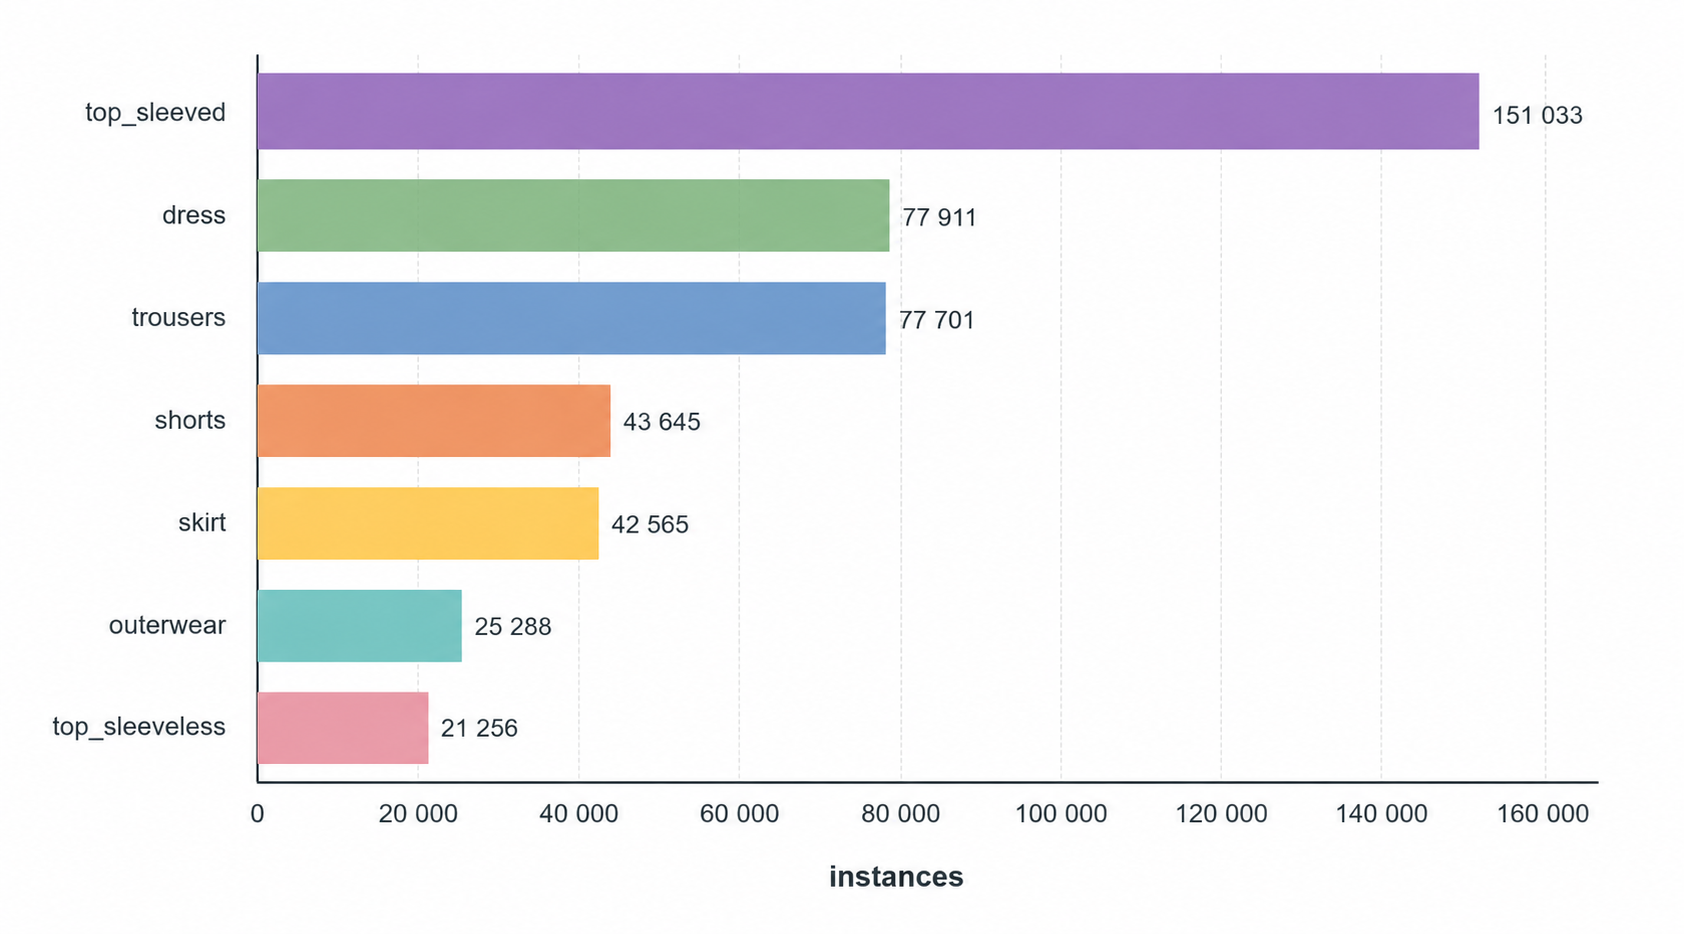
\includegraphics[width=0.90\linewidth]{datasets/merged_class_distribution.png}
  \caption{Распределение объектов по классам в объединенном датасете.}
  \label{fig:class_distribution}
\end{figure}

Рисунок~\ref{fig:class_distribution} уточняет масштаб дисбаланса: класс
\texttt{top\_sleeved} примерно в семь раз больше \texttt{top\_sleeveless}. Поэтому
поклассовые AP и confusion matrix важнее одной агрегированной mAP.

% 4.6 Геометрия изображений и bbox

\section{Геометрия изображений и bbox}

Fashion-домены имеют выраженную вертикальную ориентацию. Для DeepFashion2 средний размер
изображения составляет примерно $602.5\times756.8$ на обучающем разбиении, для Fashionpedia ---
$755.3\times986.1$, для объединенного набора --- $628.3\times795.7$. Центры \texttt{bbox}
устойчиво находятся около центра кадра: для объединенного обучающего разбиения средний центр
\texttt{bbox} равен $(0.5008, 0.5237)$, а средняя площадь \texttt{bbox} --- $0.2709$.

Это свойство имеет два следствия. С одной стороны, модель может переобучиться на центральное
расположение объектов. Поэтому при обучении применялись геометрические аугментации: перенос,
масштабирование, отражение и mosaic-подобные преобразования \cite{ultra_aug}. С другой стороны,
центральность \texttt{bbox} частично соответствует реальному стриминговому контенту с человеком
в кадре: одежда ведущего часто действительно находится в центральной области, а значит
текстурированные ROI можно стабилизировать во времени.

\begin{figure}[!htbp]
  \centering
  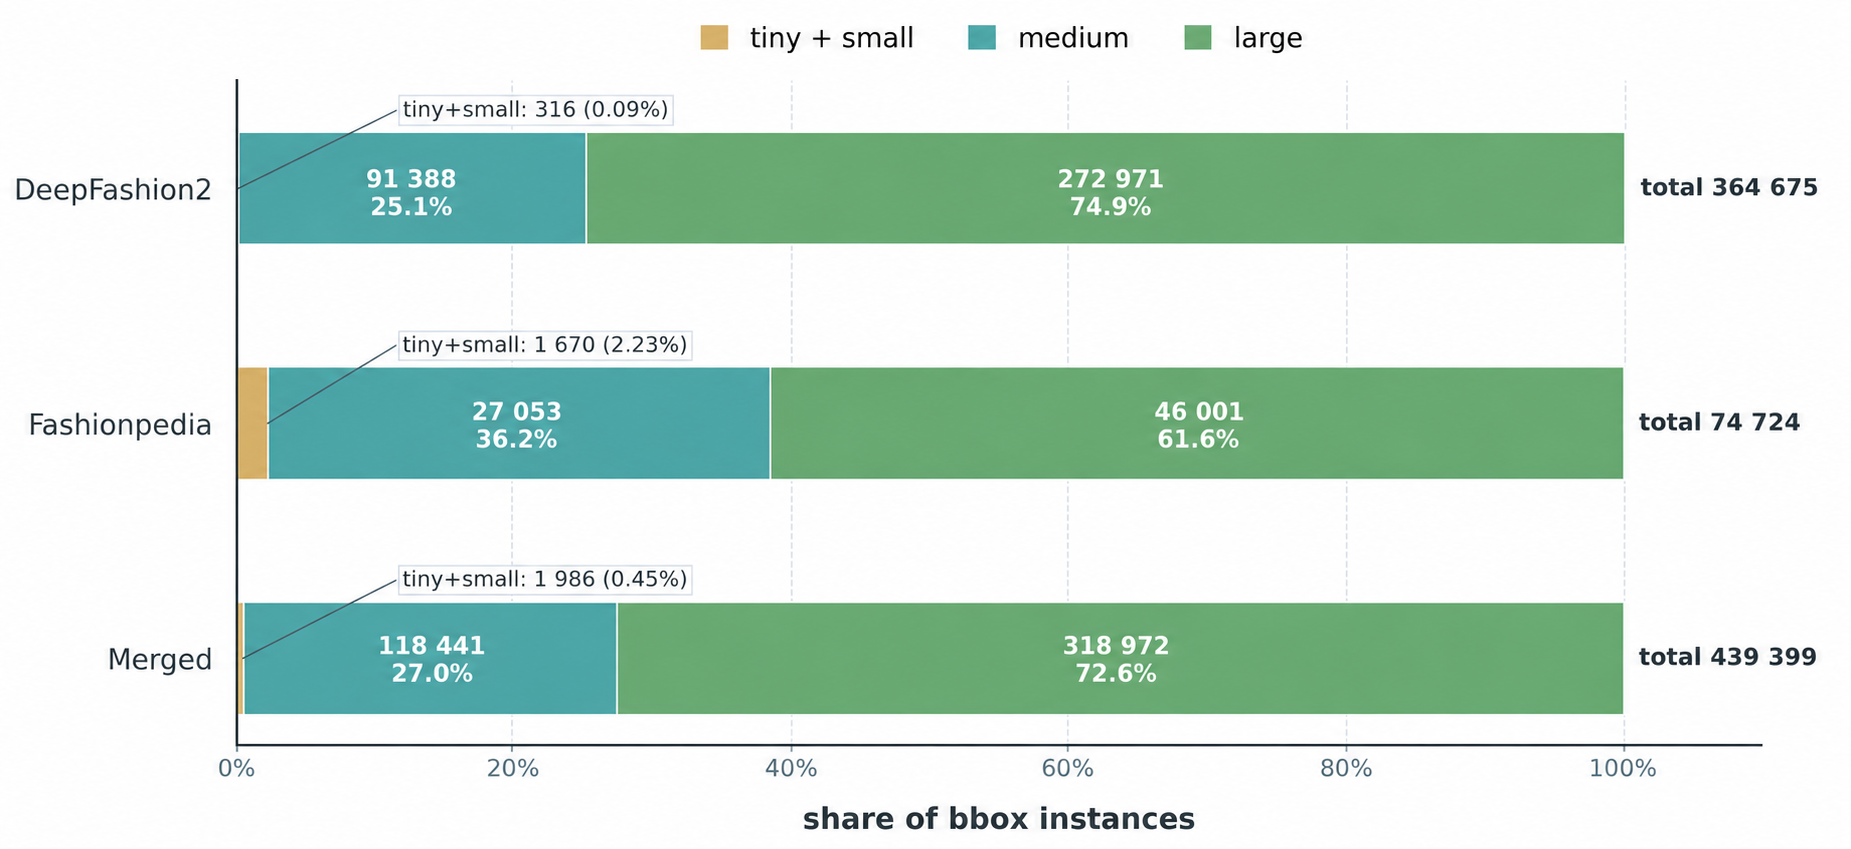
\includegraphics[width=0.86\linewidth]{datasets/bbox_area_groups.png}
  \caption{Распределение bbox по размерным группам после конвертации в YOLO-формат.}
  \label{fig:bbox_area}
\end{figure}

Рисунок~\ref{fig:bbox_area} показывает преобладание medium/large bbox во всех датасетных
вариантах. Это упрощает использование одежды как ROI-сигнала, но одновременно требует area
budget: без ограничения площади крупные области одежды могут вытеснить текст и лица.

% 4.7 Режимы обучения

\section{Режимы обучения}

В работе рассматривались следующие режимы:
\begin{enumerate}[label=\arabic*)]
  \item обучение только на DeepFashion2-7c;
  \item обучение только на Fashionpedia-7c;
  \item transfer learning: DeepFashion2 $\rightarrow$ Fashionpedia;
  \item обучение на объединенном наборе DeepFashion2 и Fashionpedia.
\end{enumerate}

На этом этапе важно подчеркнуть границу главы: здесь описываются данные, конфигурации и
воспроизводимый конвейер. Численное сравнение обученных моделей, выбор YOLO26n и анализ качества
вынесены в следующую главу, чтобы не смешивать подготовку данных с экспериментальными выводами.

% 4.8 Контракт PT-to-ONNX артефакта

\section{Контракт PT-to-ONNX артефакта}

Отдельным этапом конвейера является экспорт обученной PT-модели в ONNX. Этот этап нужен для
замыкания цикла между обучением и IDet: библиотека среды выполнения не должна зависеть от
Python-фреймворка обучения, поэтому в нее передается стабильный ONNX-артефакт с известной формой
входа, набором выходов и настройками предобработки.

\begin{figure}[!htbp]
  \centering
  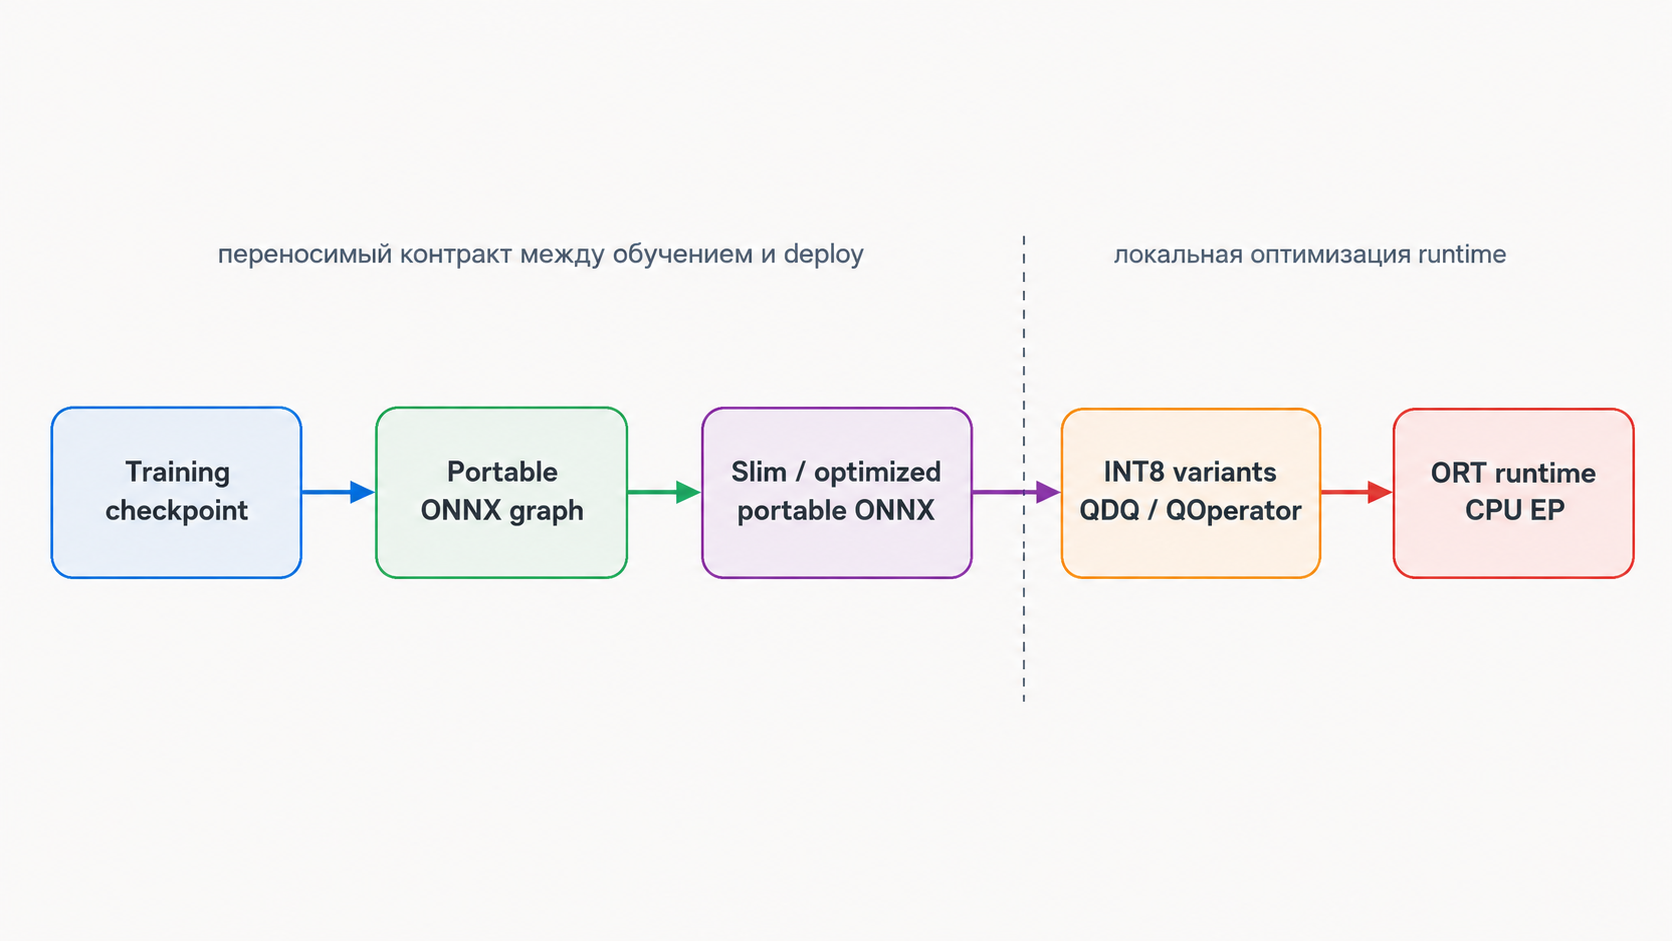
\includegraphics[width=0.96\linewidth]{yolo/pt_onnx_ort_deployment.png}
  \caption{Путь подготовки артефакта для развертывания: от обученной контрольной точки к
      переносимому ONNX и исполнению через ONNX Runtime CPU Execution Provider.}
  \label{fig:pt_onnx_ort}
\end{figure}

Рисунок~\ref{fig:pt_onnx_ort} показывает две обязательные проверки между обученной PT-точкой и
CPU-инференсом: сначала фиксируется переносимый ONNX-контракт, затем выполняется локальная
ORT-оптимизация под конкретную среду выполнения.

\begin{table}[!htbp]
  \centering
  \caption{Контракт PT-to-ONNX артефакта для детектора текстурированных ROI}
  \label{tab:pt_to_onnx_contract}
  \small
  \begin{tabularx}{\linewidth}{@{}P{0.27\linewidth}Y@{}}
    \toprule
    Элемент контракта & Требование \\
    \midrule
    Входной артефакт &
    Лучшая обучающая контрольная точка, полученная после обучения YOLO-модели на согласованной
      таксономии. \\
    Экспортируемый формат &
    ONNX-артефакт модели, совместимый с ONNX Runtime CPU Execution Provider. \\
    Размер входа &
    Фиксированная или явно задокументированная динамическая форма входа; размер должен совпадать
      с предобработкой в IDet. \\
    Параметры экспорта &
    \texttt{format=onnx}, выбранный \texttt{opset}, режим \texttt{dynamic}, \texttt{simplify},
      размер batch и флаг встроенного NMS фиксируются в отчете конвейера. \\
    Проверка корректности &
    Сравнение выходов PT и ONNX на калибровочных изображениях: форма, диапазоны уверенности,
      число кандидатов и близость координат. \\
    Проверка переносимости &
    Переносимый ONNX не должен содержать целевые узлы оптимизации раскладки ONNX Runtime,
      например \texttt{com.microsoft.nchwc::Conv}. \\
    Оптимизация &
    Сохранение версии до оптимизации и версии после оптимизации графа ORT для воспроизводимых
      измерений. \\
    Метаданные &
    Версия конвейера, YAML-описание датасета, имена классов, хэш весов и параметры
      предобработки. \\
    Интеграция &
    Артефакт регистрируется как модель адаптера текстур и используется IDet без обращения к
      Python. \\
    \bottomrule
  \end{tabularx}
\end{table}

% 4.9 ONNX Runtime и квантизация

\section{ONNX Runtime и квантизация}

После обучения модель должна пройти отдельную проверку как артефакт для развертывания. Для этого
недостаточно сохранить лучшую контрольную точку: необходимо убедиться, что экспортированный
ONNX-граф совместим с ONNX Runtime CPU Execution Provider, не содержит непереносимых внутренних
операторов раскладки и сохраняет ожидаемые формы выходов. ONNX Runtime поддерживает несколько
классов оптимизации графа и механизмы квантизации, включая QDQ и QOperator-представления
\cite{ort_graph_optim,ort_quantization}. Однако наличие INT8-артефакта само по себе не
гарантирует ускорение: итоговая скорость зависит от ядер вычисления, структуры графа, накладных
расходов деквантизации и целевой архитектуры CPU.

\begin{table}[!htbp]
  \centering
  \caption{Классификация ONNX/ORT-артефактов в конвейере}
  \label{tab:onnx_artifact_taxonomy}
  \small
  \begin{tabularx}{\linewidth}{@{}P{0.25\linewidth}P{0.25\linewidth}Y@{}}
    \toprule
    Артефакт & Роль & Основная проверка \\
    \midrule
    Raw ONNX &
    Базовый экспорт из обучающего фреймворка. &
    Формы входов/выходов, opset, отсутствие ошибок загрузки. \\
    Slimmed ONNX &
    Упрощенный переносимый граф. &
    Сохранение численной близости и структуры выходов. \\
    FP32 ONNX &
    Базовая модель для развертывания. &
    p99 задержка, размер модели, число операторов. \\
    QDQ INT8 ONNX &
    Квантизованный граф с Quantize/DeQuantize узлами. &
    Потеря качества, накладные расходы деквантизации, CPU-ядра вычисления. \\
    QOperator INT8 ONNX &
    Граф с квантизованными операторами. &
    Поддержка операторов CPU EP и отсутствие перехода на медленные пути. \\
    ORT-optimized artifact &
    Локально оптимизированный артефакт. &
    Привязка к среде выполнения/CPU; недопустимость как переносимого контракта. \\
    \bottomrule
  \end{tabularx}
\end{table}

Особое внимание нужно уделять операциям домена \texttt{com.microsoft.nchwc}. Они могут
появляться в результате внутренних оптимизаций ONNX Runtime для конкретной машины. Такой граф
полезен как целевой оптимизированный артефакт, но не должен подменять переносимый ONNX-контракт
между конвейером обучения и IDet.

% 4.10 Выводы по главе

\section{Выводы по главе}

Глава фиксирует воспроизводимый путь подготовки textured ROI детектора: исходные датасеты
приводятся к единой 7-классовой таксономии, проверяются на пропуски и некорректную разметку,
после чего используются для обучения YOLO. Локальные summary показывают, что после конвертации
нет пустых label-файлов, orphan-labels и некорректных строк разметки.

Главное ограничение данных --- дисбаланс классов и преобладание крупных bbox. Для ROI-задачи это
не делает данные непригодными, но задает условия интерпретации: нужна поклассовая проверка, а
крупные textured ROI должны проходить через ограничение площади. Экспорт в ONNX рассматривается
как отдельный deployment-контракт между YOLO-pipeline и IDet, а не как часть обучения.

% ==============================================================================
%    5. Экспериментальные результаты YOLO-моделей на объединенной таксономии
% ==============================================================================

\chapter{Экспериментальные результаты YOLO-моделей на объединенной таксономии}

% 5.1 Граница экспериментальных выводов

\section{Граница экспериментальных выводов}

В этой главе приведены результаты обучения и валидации YOLO-моделей как детекторов
текстурированных ROI. Эти результаты подтверждают качество детекции объектов на подготовленной
7-классовой таксономии, но сами по себе не доказывают рост качества видеокодирования. Для таких
выводов нужны отдельные CPU-only прогоны ONNX Runtime с p50/p90/p95/p99 задержкой и отдельный
эксперимент кодирования при одинаковом битрейте.

Поэтому численные выводы этой главы следует читать как характеристику ML-компонента. Валидация
YOLO отвечает на вопрос, способен ли детектор находить области одежды и фактуры на выбранной
таксономии. Она не отвечает на вопросы о стоимости letterbox-преобразования в C++, задержке NMS
на CPU, поведении ONNX Runtime после квантизации и том, как кодировщик перераспределит биты по
ROI.

% 5.2 Аппаратная конфигурация

\section{Аппаратная конфигурация}

Обучение выполнялось на рабочей станции с NVIDIA RTX 4090, Intel Core i9-12900F и 64 GB RAM.
Такая конфигурация позволила запускать обучение YOLO26n/YOLO26s с тяжелыми аугментациями и
большим merged dataset. RTX 4090 имеет 24 GB видеопамяти, что делает ее практичной для обучения
современных моделей компьютерного зрения \cite{nvidia4090}.

Эта конфигурация относится именно к обучению и валидации YOLO-моделей. CPU-only измерения IDet
выполнялись отдельно, уже после экспорта моделей в ONNX и переноса в C++/ONNX Runtime контур.
Такое разделение важно: GPU-станция проверяет качество ML-компонента, а серверные CPU-прогоны
показывают стоимость будущего runtime-исполнения.

\begin{table}[!htbp]
  \centering
  \caption{Аппаратная конфигурация обучения}
  \label{tab:hardware}
  \begin{tabularx}{\linewidth}{@{}Y Y@{}}
    \toprule
    Компонент & Значение \\
    \midrule
    GPU & NVIDIA RTX 4090, 24 GB VRAM \\
    CPU & Intel Core i9-12900F, 16 Cores, 24 Threads \\
    RAM & 64 GB DDR5\\
    Модели & YOLO26n, YOLO26s \\
    Основной кандидат для IDet & YOLO26n \\
    \bottomrule
  \end{tabularx}
\end{table}

YOLO26n выбран как основной кандидат не потому, что он максимизирует все метрики, а потому что
дает достаточное качество при меньшей вычислительной стоимости. Для CPU-ориентированной
библиотеки этот критерий важнее небольшого прироста mAP у более тяжелой модели.

% 5.3 Итоговые метрики YOLO26n

\section{Итоговые метрики YOLO26n}

Итоговые метрики YOLO26n на объединенной 7-классовой таксономии приведены в
таблице~\ref{tab:yolo_metrics}. По результатам валидационного отчета модель достигла mAP@0.5 =
0.938 и mAP@0.5:0.95 = 0.818 при precision = 0.903 и recall = 0.873. Для легкой модели это
сильный результат, особенно с учетом дальнейшей CPU-интеграции. При этом в доступных отчетах нет
подтвержденного значения оптимального F1-порога, поэтому F1 не используется как отдельный
численный вывод.

\begin{table}[!htbp]
  \centering
  \caption{Итоговые метрики YOLO26n на объединенной 7-классовой таксономии}
  \label{tab:yolo_metrics}
  \begin{tabularx}{\linewidth}{@{}Y Z Y Z@{}}
    \toprule
    Метрика & Значение & Метрика & Значение \\
    \midrule
    Precision & 0.903 & Recall & 0.873 \\
    mAP@0.5 & 0.938 & mAP@0.5:0.95 & 0.818 \\
    \bottomrule
  \end{tabularx}
\end{table}

Сочетание высокой AP@0.5 и заметно более строгой mAP@0.5:0.95 показывает, что модель уверенно
находит объекты одежды, но качество точной геометрии bbox остается отдельным фактором риска для
ROI-кодирования.

% 5.4 Поклассовая точность детектора

\section{Поклассовая точность детектора}

Поклассовая AP показывает, что модель наиболее уверенно распознает \texttt{trousers},
\texttt{dress}, \texttt{top\_sleeved}, \texttt{shorts} и \texttt{skirt}. Более сложными являются
\texttt{top\_sleeveless} и \texttt{outerwear}. Это ожидаемо: \texttt{top\_sleeveless} менее
представлен и визуально близок к другим верхним классам, а \texttt{outerwear} часто пересекается
с \texttt{top\_sleeved} и \texttt{dress}.

Для ROI-задачи особенно важно сравнивать AP@0.5 и AP@0.5:0.95 вместе. Если AP@0.5 высокий, а
строгая AP заметно ниже, модель в целом находит объект, но геометрия bbox менее точна. В обычной
классификации одежды это может быть вторичным, но для кодировщика геометрия напрямую задает
защищаемую площадь. Поэтому классы с низкой строгой AP требуют downstream-ограничений: clipping,
area cap или более консервативный qoffset.

На рисунке~\ref{fig:yolo_per_class_ap_comparison} приведено поклассовое сравнение метрик AP50 и
AP50-95 для четырех обучающих конфигураций YOLO26. В отличие от диагональных значений confusion
matrix, данные метрики учитывают не только правильность выбора класса, но и качество локализации
bbox. AP50 отражает качество детекции при пороге IoU = 0.5, тогда как AP50-95 является более
строгой метрикой, усредненной по нескольким порогам IoU от 0.5 до 0.95.

Такое сравнение позволяет оценить, какие классы остаются устойчивыми при смене модели и
датасета, а какие сильнее теряют качество при более строгой оценке локализации.

\begin{figure}[!htbp]
  \centering
  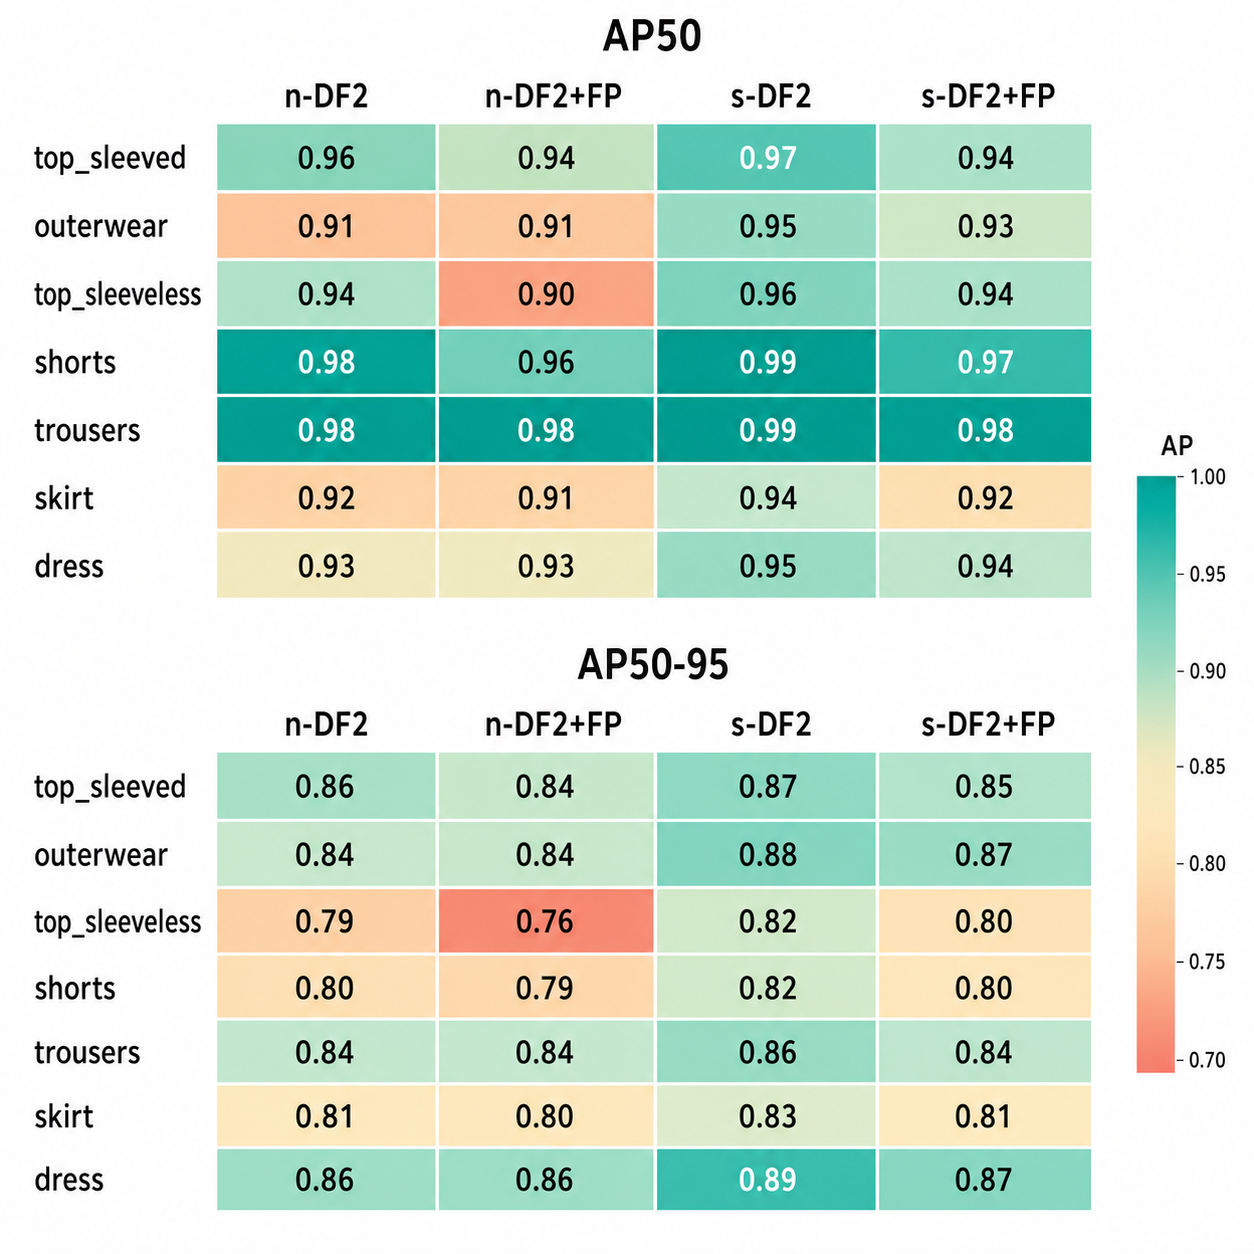
\includegraphics[width=0.86\linewidth]{yolo/yolo_ap_per_class_comparison.png}
  \caption{Поклассовые значения AP50 и AP50-95 для четырех YOLO-конфигураций: YOLO26n и YOLO26s на
      DeepFashion2-7c и объединенном наборе DeepFashion2+Fashionpedia-7c.}
  \label{fig:yolo_per_class_ap_comparison}
\end{figure}

Рисунок~\ref{fig:yolo_per_class_ap_comparison} показывает, что во всех конфигурациях значения
AP50 заметно выше, чем AP50-95. Для textured ROI это существенный результат: модель часто
находит нужный объект, но строгая геометрия остается отдельным риском для кодировщика.

Наиболее устойчивыми классами остаются \texttt{top\_sleeved}, \texttt{trousers} и
\texttt{dress}: они сохраняют высокие значения AP в разных конфигурациях. Более сложными
оказываются \texttt{top\_sleeveless}, \texttt{shorts} и часть случаев \texttt{skirt}, где
снижение AP50-95 указывает на более чувствительную локализацию bbox.

Сравнение YOLO26n и YOLO26s показывает, что более тяжелая модель в целом дает более высокое
качество, особенно по строгой метрике AP50-95. Однако этот прирост необходимо сопоставлять с
вычислительной стоимостью: YOLO26s имеет больше параметров и GFLOPs, поэтому для CPU-first
сценария YOLO26n может оставаться более предпочтительным компромиссом. Объединенный набор
DeepFashion2+Fashionpedia делает проверку модели более строгой за счет большего разнообразия
данных, поэтому небольшое снижение отдельных поклассовых AP не противоречит его практической
ценности для textured ROI.

% 5.5 Сравнение YOLO26n и YOLO26s

\section{Сравнение YOLO26n и YOLO26s}

Сравнение YOLO26n и YOLO26s показывает ожидаемый компромисс между качеством и вычислительной
стоимостью. YOLO26s имеет около 9.47 млн параметров и 20.5 GFLOPs против 2.38 млн параметров и
5.2 GFLOPs у YOLO26n, то есть примерно четырехкратную вычислительную стоимость по валидационным
отчетам. На DeepFashion2 это дает рост mAP@0.5:0.95 с 0.829 до 0.850. На объединенном наборе
сохраненные отчеты показывают 0.818 для YOLO26n и 0.837 для YOLO26s.

Это сравнение необходимо трактовать осторожно, потому что число валидационных изображений и
объектов в отдельных сохраненных отчетах различается. Тем не менее общий вывод устойчив: более
тяжелая модель дает умеренный прирост качества, но хуже соответствует CPU-ориентированной роли
IDet. Для ВКР важнее не абсолютный максимум mAP, а возможность встроить детектор в конвейер
реального времени с жестким бюджетом на всю предобработку и постобработку.

\begin{figure}[!htbp]
  \centering
  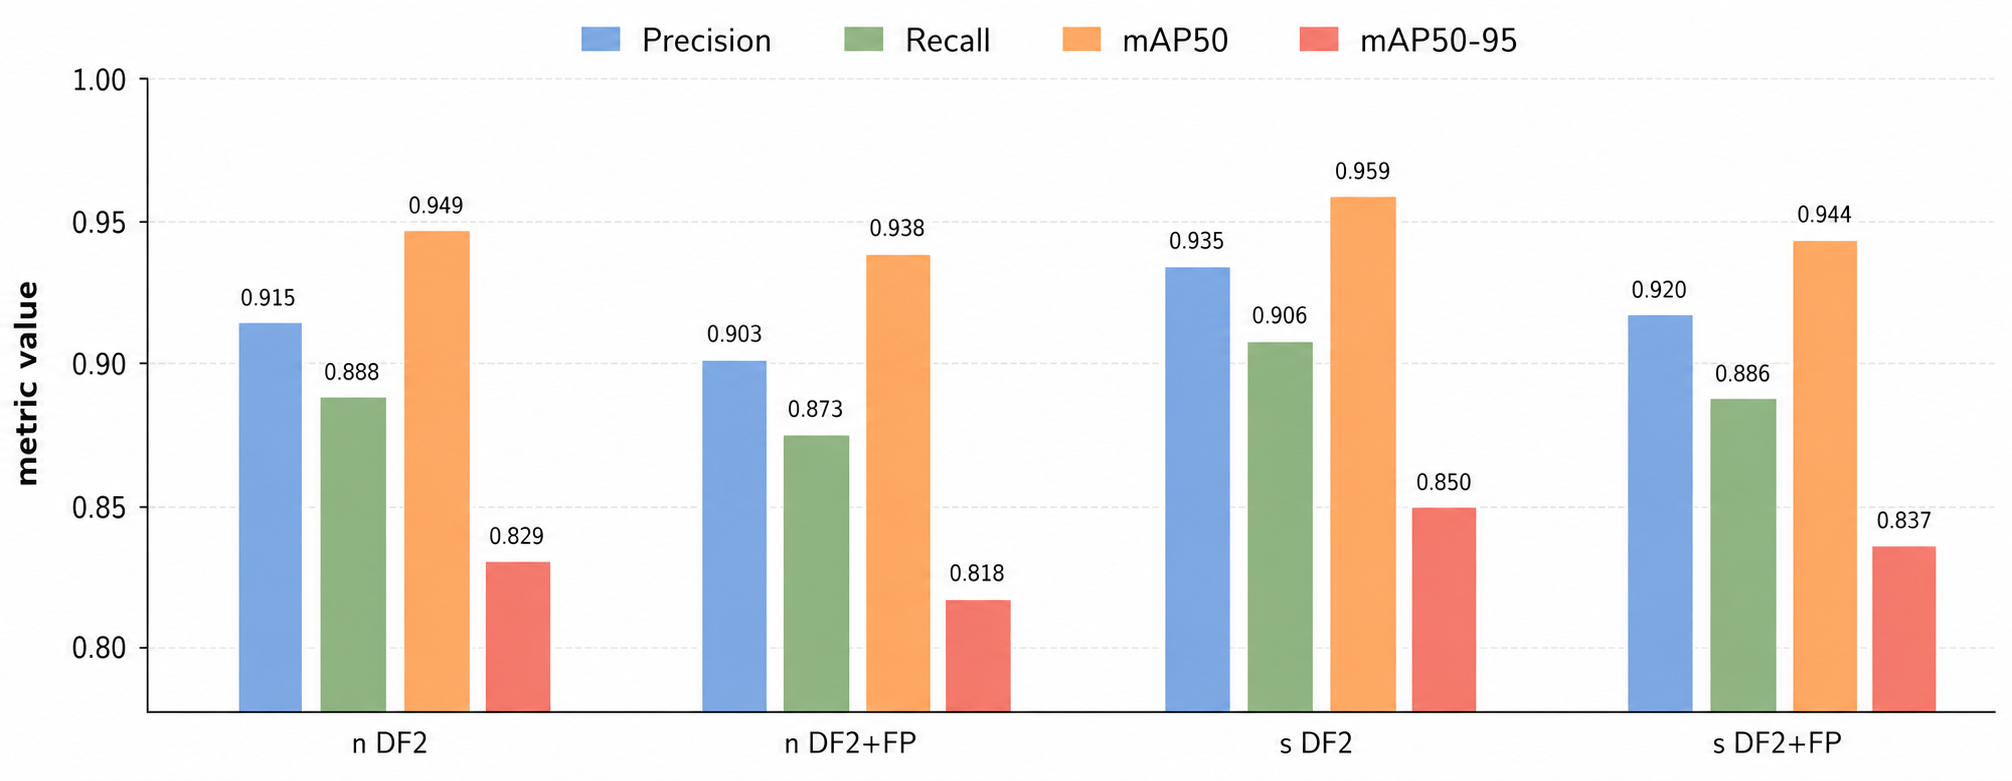
\includegraphics[width=0.90\linewidth]{yolo/yolo_model_metrics_comparison.png}
  \caption{Сравнение precision, recall, mAP@0.5 и mAP@0.5:0.95 для YOLO26n/YOLO26s по сохраненным
      валидационным сводкам.}
  \label{fig:model_comparison}
\end{figure}

Рисунок~\ref{fig:model_comparison} показывает умеренное преимущество YOLO26s по строгой mAP, но
этот прирост не меняет порядок величины качества. Для CPU-first интеграции его недостаточно,
чтобы автоматически выбрать более тяжелую модель.

\begin{figure}[!htbp]
  \centering
  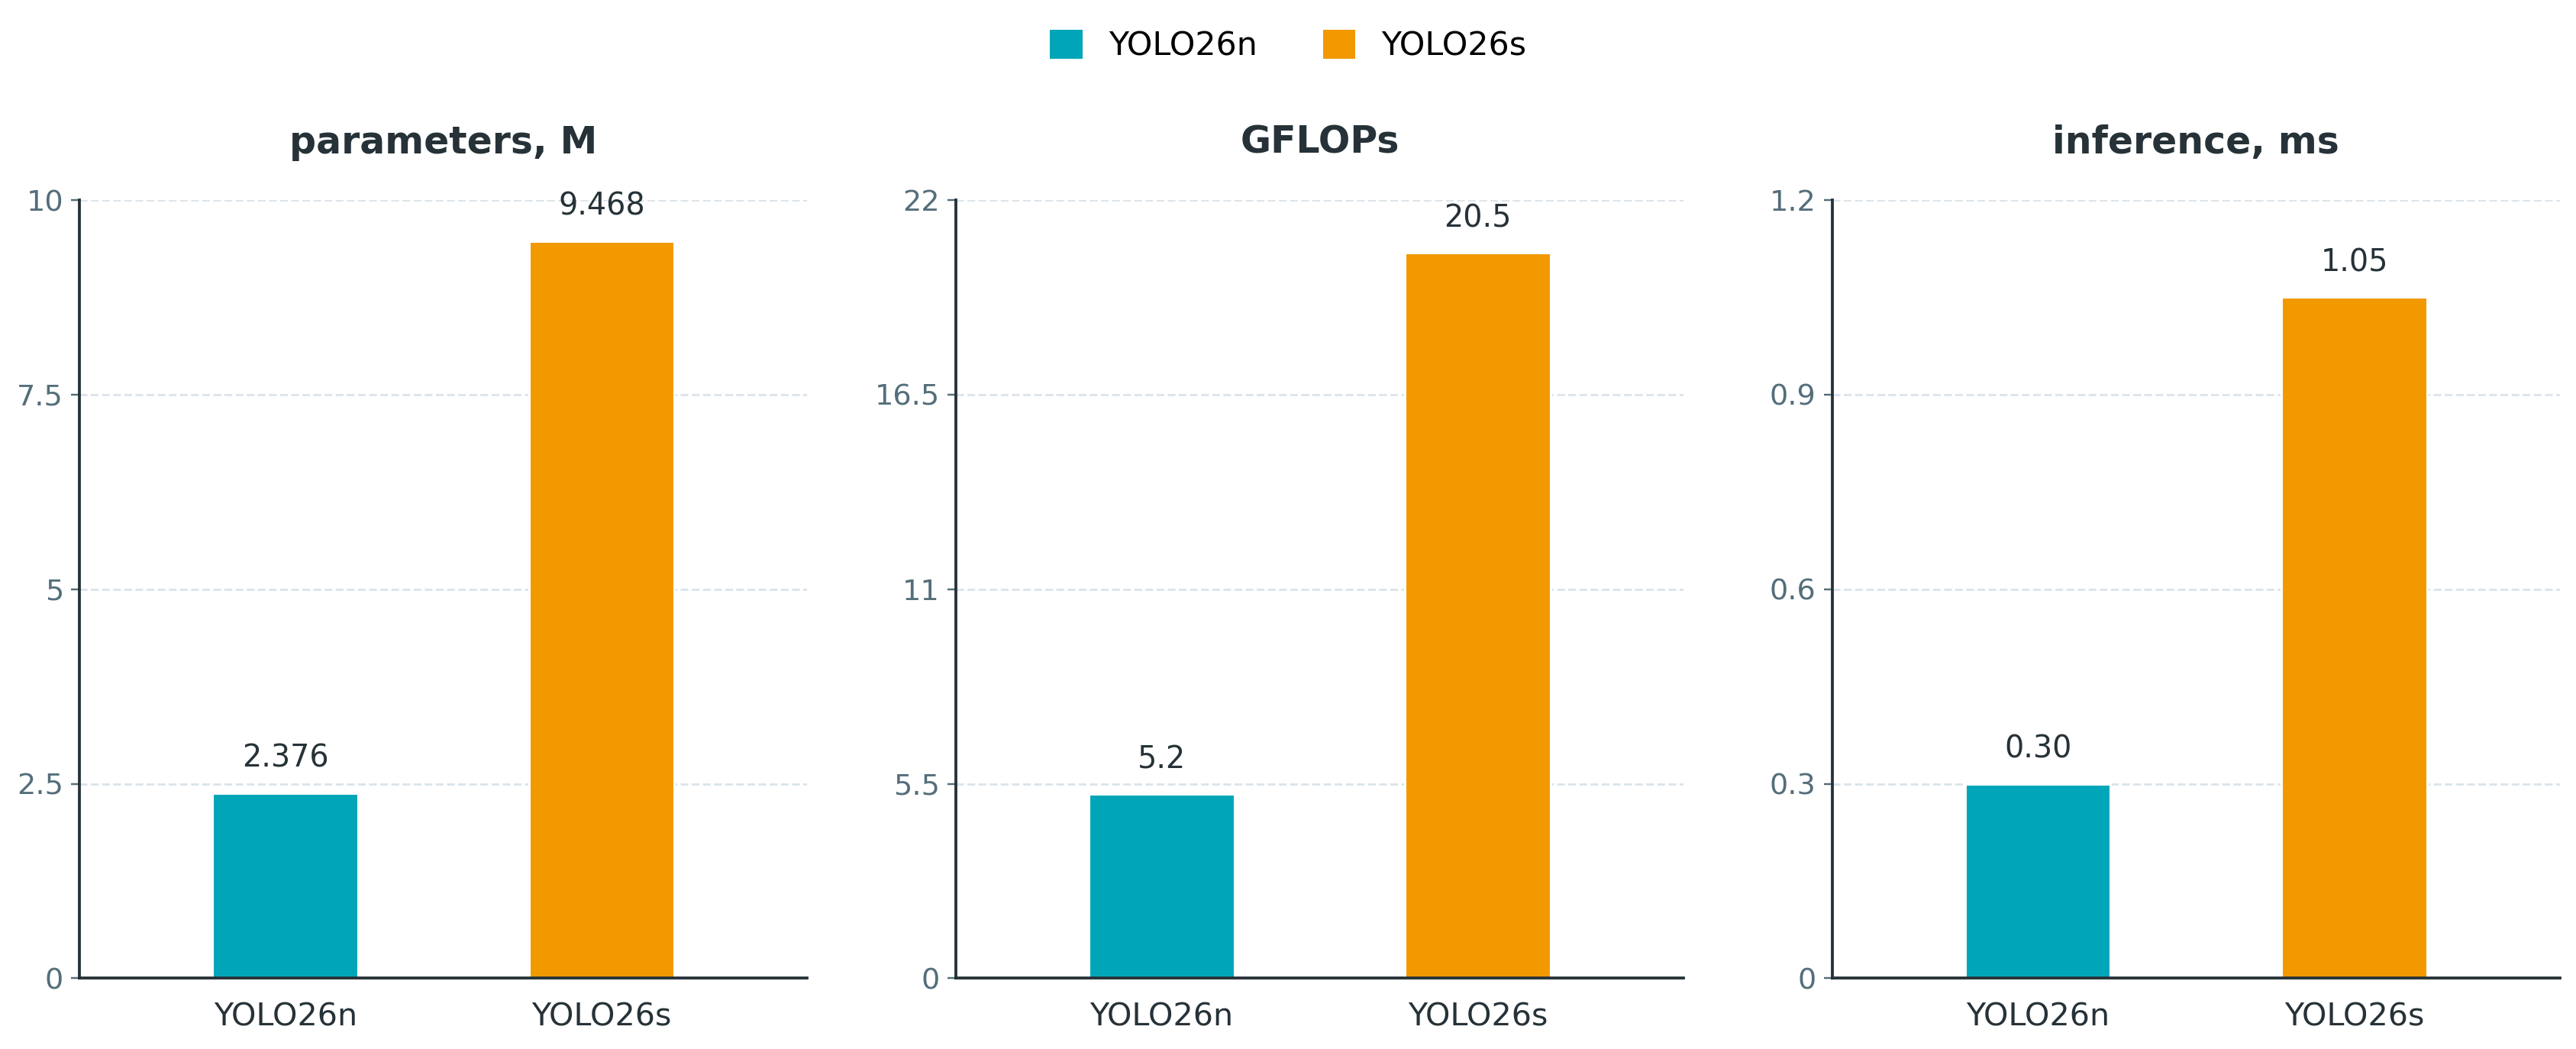
\includegraphics[width=0.86\linewidth]{yolo/yolo_model_cost_comparison.png}
  \caption{Сравнение параметров и GFLOPs для YOLO26n и YOLO26s.}
  \label{fig:model_cost}
\end{figure}

На рисунке~\ref{fig:model_cost} видно, что вычислительная цена YOLO26s примерно в четыре раза
выше по параметрам и GFLOPs. Поэтому даже небольшой прирост mAP нужно проверять через p99
полного IDet-конвейера, а не только через валидационный отчет Ultralytics.

% 5.6 Матрица ошибок

\section{Матрица ошибок}

Нормализованная матрица ошибок показывает, что на диагонали модель имеет сильные значения:
$0.92$ для \texttt{top\_sleeved}, $0.95$ для \texttt{trousers}, $0.90$ для \texttt{shorts} и
$0.87$ для \texttt{dress}. Более низкие значения у \texttt{top\_sleeveless} ($0.80$) и
\texttt{outerwear} ($0.83$) объясняются визуальной близостью классов и дисбалансом данных.
Заметная часть ошибок связана не с заменой одного класса одежды другим, а с фоном: это означает,
что часть одежды может не получить текстурированную ROI, если пороги и политика площади выбраны
слишком агрессивно.

\begin{figure}[!htbp]
  \centering
  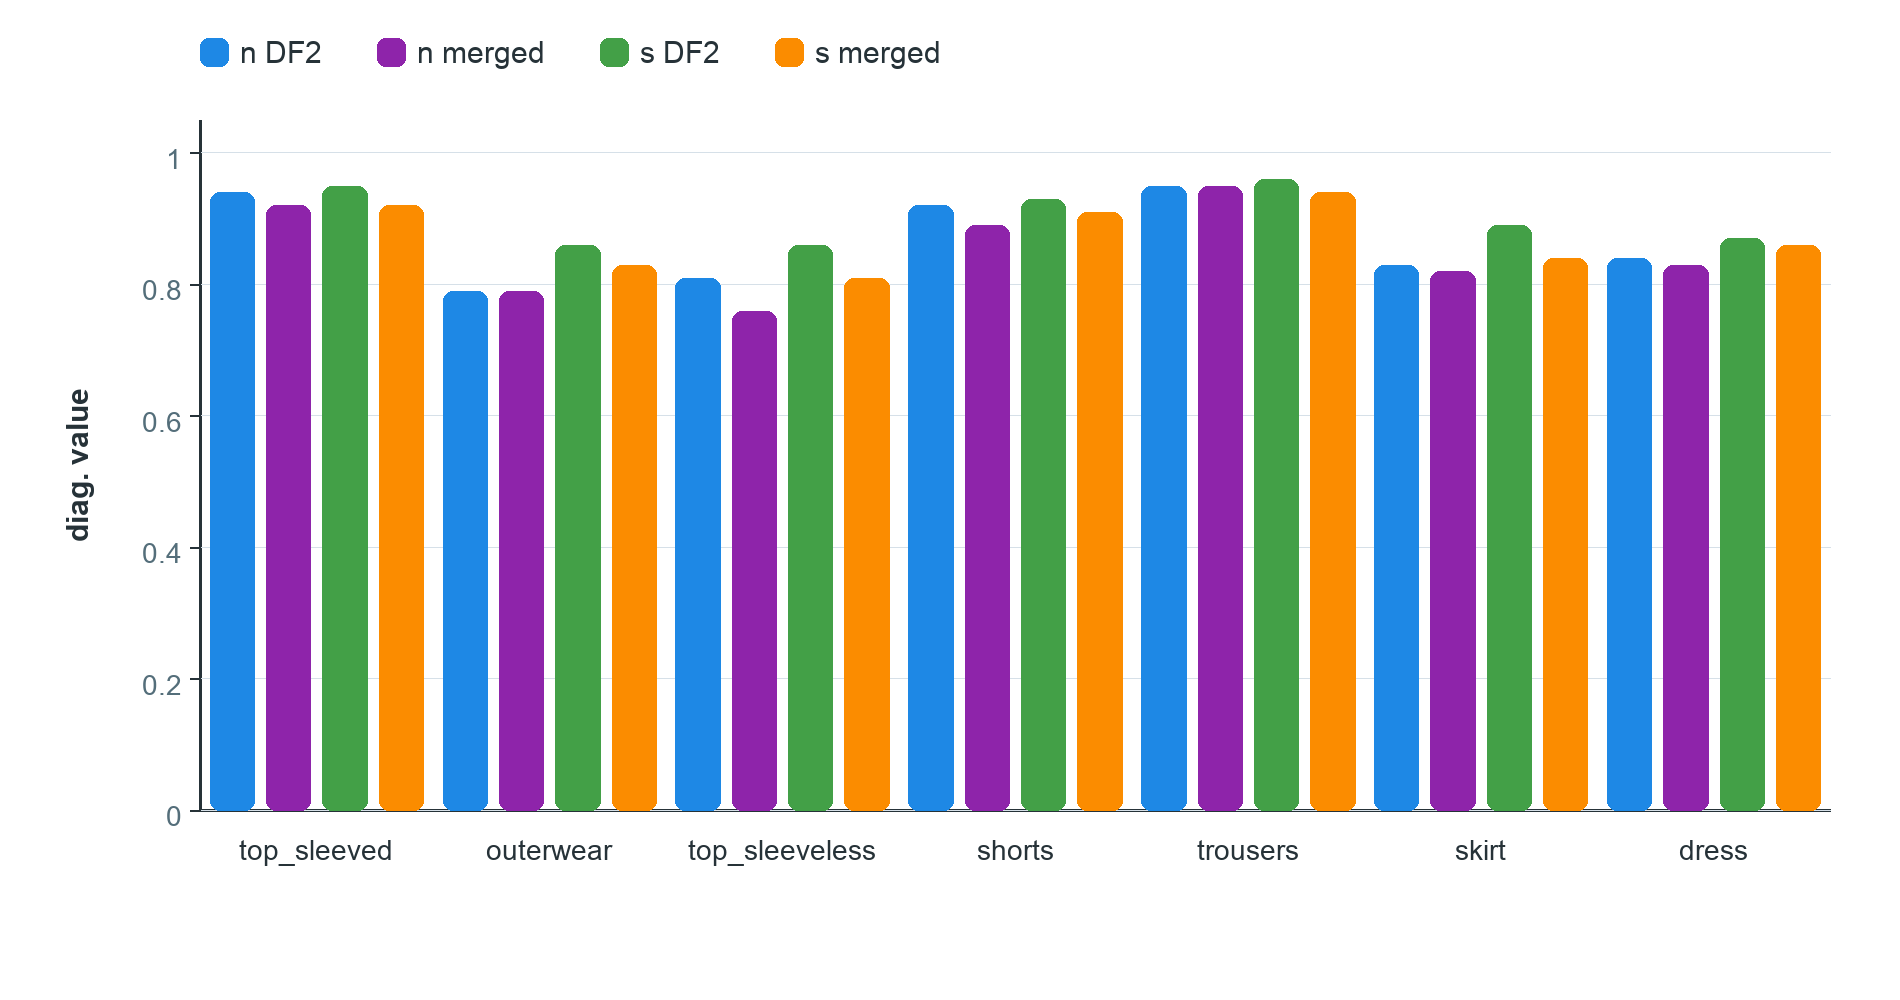
\includegraphics[width=0.75\linewidth]{yolo/yolo_confusion_diagonal_comparison.png}
  \caption{Сравнение диагональных значений нормализованных матриц ошибок для четырех
      YOLO-экспериментов.}
  \label{fig:confusion_diag_compare}
\end{figure}

Рисунок~\ref{fig:confusion_diag_compare} показывает, что наиболее устойчивы
\texttt{trousers}, \texttt{top\_sleeved} и \texttt{dress}; слабее выглядят
\texttt{top\_sleeveless} и \texttt{outerwear}. Эти классы должны оставаться в фокусе при выборе
порогов уверенности и area policy.

Для задачи формирования ROI-кандидатов часть ошибок между близкими классами одежды менее
критична, чем полный пропуск области. Если модель перепутала юбку и платье, но корректно
выделила область одежды, кодировщик все равно получает полезный сигнал. Более опасны ошибки
другого типа: одежда как фон или фон как текстурированная ROI. Поэтому матрица ошибок в данной
работе интерпретируется не как тонкая классификация модных категорий, а как диагностика
отделения переднего плана от фона и покрытия ROI.

% 5.7 Сводка артефактов для развертывания

\section{Сводка артефактов для развертывания}

Помимо обучающих сводок, важен срез качества, ориентированный на развертывание. В опубликованной
сводке артефактов для YOLO26 фиксируется входной размер 640, динамический пространственный вход,
ONNX Runtime CPU Execution Provider и разные FP32/INT8-представления. Такая сводка показывает не
только mAP, точность и полноту, но и размер модели для развертывания, поведение квантизованных
вариантов и пригодность артефакта для CPU-среды выполнения.

\begin{table}[!htbp]
  \centering
  \caption{FP32-артефакты YOLO26 для CPU-среды выполнения}
  \label{tab:yolo_model_zoo_artifacts}
  \scriptsize
  \begin{tabularx}{\linewidth}{@{}P{0.10\linewidth}P{0.25\linewidth}Z Z Z Z Z@{}}
    \toprule
    Модель & Датасет & mAP50-95 & mAP50 & Precision & Recall & Mem, MB \\
    \midrule
    YOLO26n & DeepFashion2 & 0.8131 & 0.9343 & 0.8974 & 0.8767 & 9.3 \\
    YOLO26n & DeepFashion2+Fashionpedia & 0.8202 & 0.9395 & 0.9319 & 0.8621 & 9.3 \\
    YOLO26s & DeepFashion2 & 0.8364 & 0.9490 & 0.9167 & 0.8940 & 36.4 \\
    YOLO26s & DeepFashion2+Fashionpedia & 0.8161 & 0.9225 & 0.8982 & 0.8620 & 36.4 \\
    \bottomrule
  \end{tabularx}
\end{table}

\begin{table}[!htbp]
  \centering
  \caption{INT8-варианты YOLO26 для CPU-среды выполнения}
  \label{tab:yolo_model_zoo_int8}
  \scriptsize
  \begin{tabularx}{\linewidth}{@{}P{0.10\linewidth}P{0.25\linewidth}Z Z Z Z Z@{}}
    \toprule
    Модель & Датасет & mAP50-95 & mAP50 & Precision & Recall & Mem, MB \\
    \midrule
    YOLO26n &
    DeepFashion2 &
    0.7466--0.7492 &
    0.8848--0.8863 &
    0.8211--0.8261 &
    0.9038--0.9058 &
    2.7--2.9 \\
    YOLO26n &
    DeepFashion2+Fashionpedia &
    0.7421--0.7437 &
    0.8723--0.8736 &
    0.9373--0.9404 &
    0.7978--0.7984 &
    2.7--2.9 \\
    YOLO26s &
    DeepFashion2 &
    0.8158--0.8167 &
    0.9403--0.9414 &
    0.9203--0.9256 &
    0.8817--0.8826 &
    9.6--9.8 \\
    YOLO26s &
    DeepFashion2+Fashionpedia &
    0.7707--0.7740 &
    0.8968--0.9000 &
    0.8980--0.9018 &
    0.8465--0.8492 &
    9.6--9.8 \\
    \bottomrule
  \end{tabularx}
\end{table}

Из таблицы видно, что квантизация резко уменьшает размер артефакта: для YOLO26n примерно с 9.3
MB до 2.7--2.9 MB, для YOLO26s --- с 36.4 MB до 9.6--9.8 MB. Однако это сопровождается заметной
потерей mAP50-95, особенно для объединенного набора. Поэтому INT8-варианты в данной работе
рассматриваются как гипотезы развертывания, требующие отдельной проверки задержки и качества, а
не как автоматически лучший выбор.

% 5.8 Почему выбран YOLO26n

\section{Почему выбран YOLO26n}

Финальное инженерное решение --- выбрать YOLO26n как основной кандидат для текстурированных ROI
в IDet. YOLO26s может давать более высокую точность в части экспериментов, но требует около 20.5
GFLOPs против 5.2 GFLOPs у YOLO26n. Цель ВКР --- не построить максимально точный
fashion-классификатор, а получить модель, которую реалистично встроить в CPU-ориентированную
IDet и проверить в режиме с ограниченным бюджетом на всю предобработку и постобработку.

Этот выбор также подтверждается сводкой артефактов для развертывания. При одинаковом входном
размере и CPU Execution Provider FP32-артефакт YOLO26n для объединенного набора занимает 9.3 MB
и показывает mAP50-95 = 0.8202, тогда как FP32-артефакт YOLO26s занимает 36.4 MB и в этой сводке
не дает устойчивого преимущества на объединенном наборе. Это не отменяет того, что в отдельных
обучающих сводках YOLO26s может быть точнее; это показывает другое: после перевода в контракт
развертывания легкая модель выглядит более подходящей для CPU-ориентированной среды выполнения.

\begin{figure}[!htbp]
  \centering
  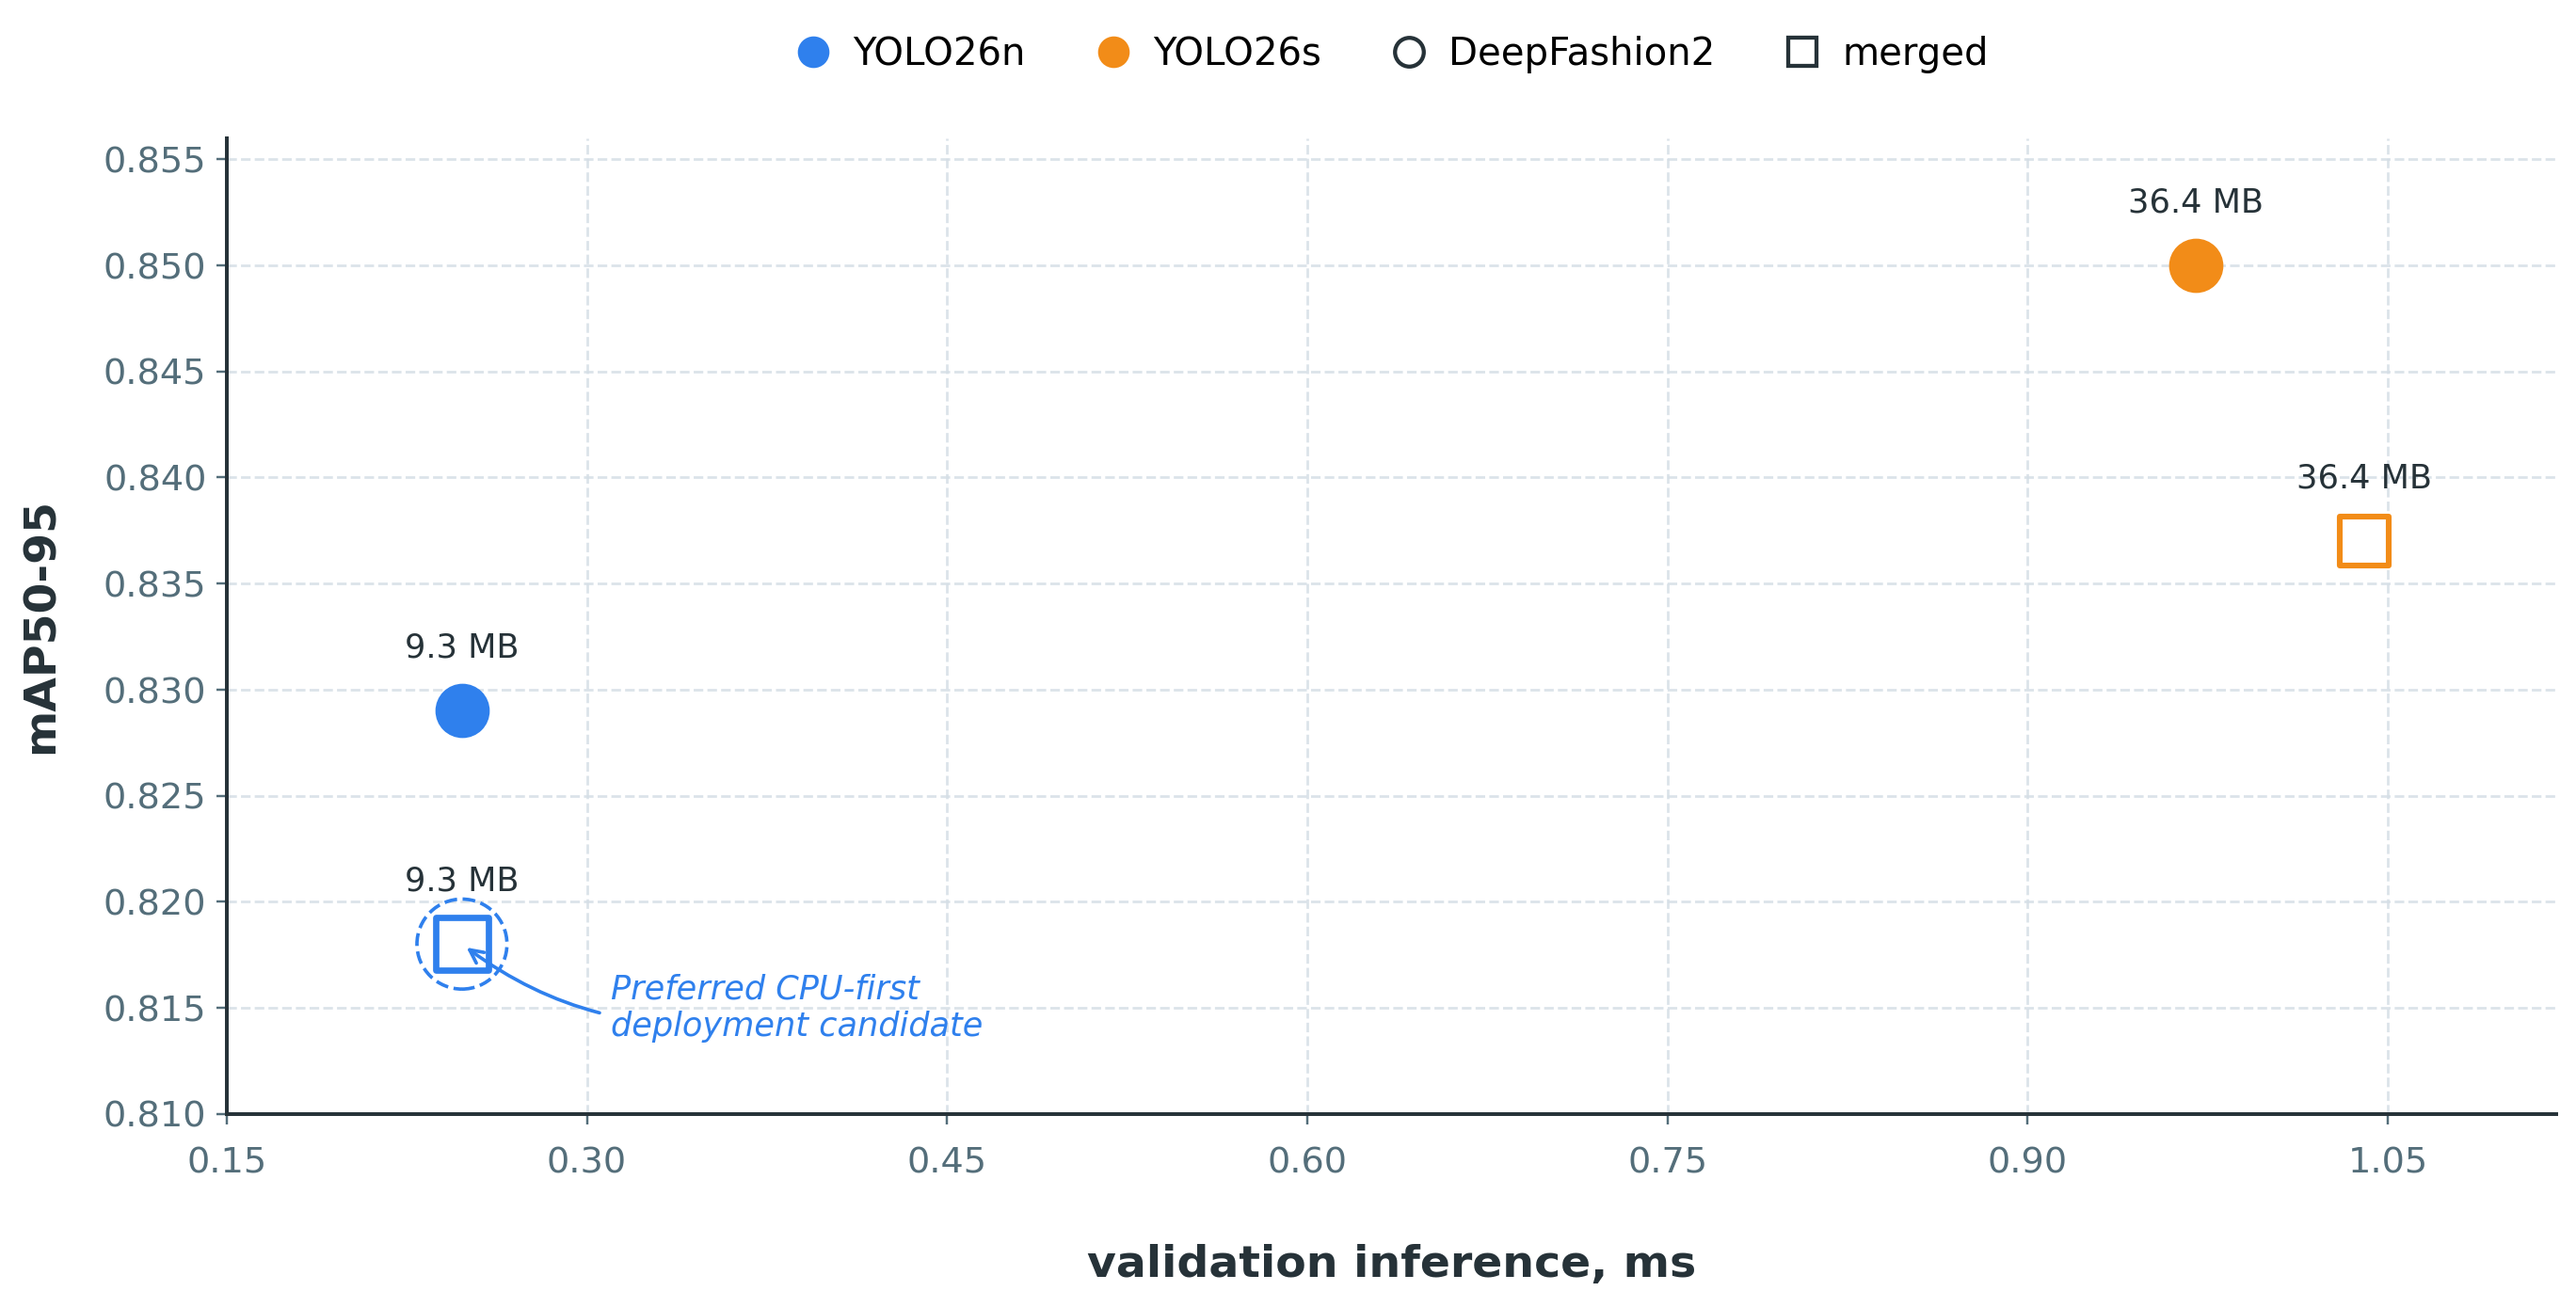
\includegraphics[width=0.82\linewidth]{yolo/yolo_quality_cost_tradeoff.png}
  \caption{Компромисс между качеством детектора и вычислительной стоимостью по валидационным
      отчетам.}
  \label{fig:quality_latency}
\end{figure}

Рисунок~\ref{fig:quality_latency} суммирует deployment-компромисс: YOLO26n сохраняет качество,
близкое к YOLO26s, но имеет существенно меньший размер и расчетную стоимость.

% 5.9 Выводы по главе

\section{Выводы по главе}

YOLO26n на объединенной таксономии достигает precision $0.903$, recall $0.873$,
mAP@0.5 $0.938$ и mAP@0.5:0.95 $0.818$. Эти значения достаточны, чтобы рассматривать модель как
кандидат для textured ROI, но не являются доказательством улучшения видео: они проверяют только
ML-компонент.

Сравнение с YOLO26s показывает последовательный компромисс. Более тяжелая модель может быть
точнее в обучающих отчетах, но стоит примерно в четыре раза дороже по параметрам и GFLOPs.
Поэтому для CPU-ориентированной IDet выбран YOLO26n: он дает близкое качество, меньший
deployment-артефакт и более реалистичную основу для дальнейших p99-измерений.

% ==============================================================================
%                    6. Интеграция ROI в видеокодирование
% ==============================================================================

\chapter{Интеграция ROI в видеокодирование}

% 6.1 ROI как управляющий сигнал

\section{ROI как управляющий сигнал}

В данной работе ROI-детектор не является финальным продуктом сам по себе. Его выход --- это
управляющий сигнал для кодировщика. Поэтому система должна оцениваться не только по detection
metrics, но и по тому, как ROI может быть использован для перераспределения качества при
фиксированном битрейте.

Пусть $V$ --- исходное видео, $D$ --- ROI-детектор, $S$ --- политика приоритизации и
преобразования ROI в управляющую информацию для кодировщика, а $E$ --- кодировщик. Тогда полный
конвейер можно записать как
\begin{equation}
  \hat{V} = E(V, S(D(V))),
  \label{eq:pipeline}
\end{equation}
где $\hat{V}$ --- закодированный и восстановленный видеопоток. В этой постановке детектор $D$ не
оптимизируется изолированно: он должен быть полезен внутри кодировщика $E$.

Такое разделение важно для корректной интерпретации результатов. Высокая mAP детектора
текстурированных ROI означает, что модель хорошо находит объекты одежды на валидационном
разбиении. Но итоговая польза для видеостриминга возникает только тогда, когда эти области
корректно преобразуются в \texttt{qoffset}/метаданные ROI и действительно влияют на
распределение битового бюджета.

% 6.2 Адаптер кодировщика как граница между IDet и кодировщиком

\section{Адаптер кодировщика как граница между IDet и кодировщиком}

Интеграционный слой должен быть отделен от детекторов. Модель не должна знать, работает ли
кодировщик через метаданные ROI FFmpeg, адаптивное квантование или резервную предобработку фона.
FFmpeg \texttt{addroi} прикрепляет к кадру метаданные об областях интереса, не изменяя пиксели
самого кадра, а \texttt{AVRegionOfInterest} задает координаты и \texttt{qoffset} для таких
областей \cite{ffmpeg_roi,ffmpeg_addroi}. Это делает адаптер кодировщика естественной границей
между компьютерным зрением и видеокодированием.

\begin{figure}[!htbp]
  \centering
  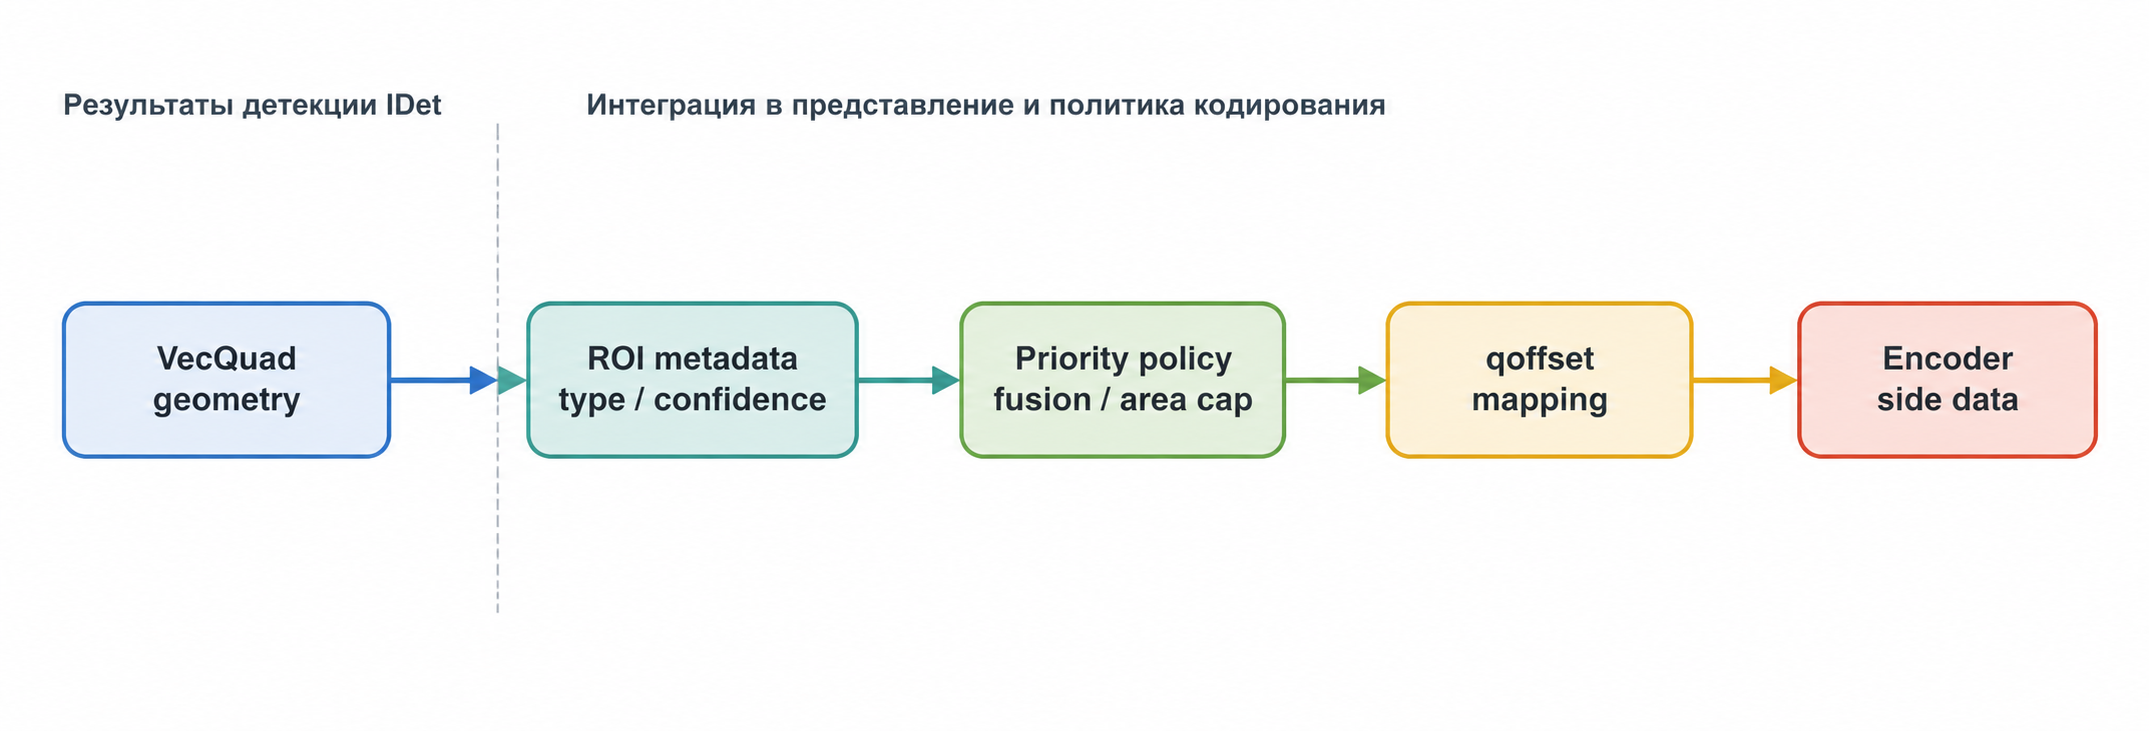
\includegraphics[width=0.96\linewidth]{architecture/encoder_roi_mapping.png}
  \caption{Преобразование метаданных ROI в управляющую информацию для кодировщика: ограничение
      площади, сортировка, отображение в \texttt{qoffset} и передача ROI side data.}
  \label{fig:encoder_mapping}
\end{figure}

Рисунок~\ref{fig:encoder_mapping} показывает, что адаптер кодировщика должен получать уже
отсортированные и ограниченные по площади ROI. Иначе \texttt{qoffset} будет применяться к
слишком большим или конфликтующим областям, что ухудшит фон и израсходует битовый бюджет.

\begin{table}[!htbp]
  \centering
  \caption{Алгоритмический контракт адаптера кодировщика}
  \label{tab:encoder_adapter_contract}
  \begin{tabularx}{\linewidth}{@{}P{0.22\linewidth}Y@{}}
    \toprule
    Операция & Семантика \\
    \midrule
    \texttt{supportsROI} & Проверка поддержки ROI side data или карты \texttt{qoffset}. \\
    \texttt{mapPriority} & Преобразование приоритета ROI в управляющую подсказку кодировщику. \\
    \texttt{applyHints} & Передача ROI после ограничения площади и сортировки. \\
    \texttt{fallback} & Резервная стратегия при отсутствии нативной ROI-поддержки. \\
    \bottomrule
  \end{tabularx}
\end{table}

Этот адаптер позволяет сохранить модульность: IDet отвечает за поиск областей, ROI-слой --- за
слияние и стабилизацию, адаптер кодировщика --- за конкретный способ влияния на кодирование.

% 6.3 Политика qoffset

\section{Политика qoffset}

Для каждой ROI задается приоритет $p_i$. Сильнее всего защищается текст, затем лица, затем
текстурированные ROI. Практическая политика может быть задана таблицей~\ref{tab:qoffset_policy}.

\begin{table}[!htbp]
  \centering
  \caption{Пример политики приоритизации ROI}
  \label{tab:qoffset_policy}
  \begin{tabularx}{\linewidth}{@{}Y Z Z Y@{}}
    \toprule
    Тип ROI & Priority & qoffset & Причина \\
    \midrule
    Текстовая ROI & 1.00 & -0.20 & Читаемость текста критична для пользователя. \\
    ROI лица & 0.85 & -0.15 & Искажения лица заметны субъективно. \\
    Текстурированная ROI & 0.55 & -0.08 & Фактура важна, но не должна вытеснять текст/лицо. \\
    Фон & 0.00 & 0.00 & Фон кодируется без дополнительной защиты. \\
    \bottomrule
  \end{tabularx}
\end{table}

Эти значения не являются универсальными константами. Они задают начальную инженерную политику
для экспериментов. В реальной системе \texttt{qoffset} следует подбирать на валидационном
видеокорпусе с учетом битрейта, кодека, типа контента и допустимого ухудшения фоновых областей.

% 6.4 Ограничение площади и разрешение конфликтов

\section{Ограничение площади и разрешение конфликтов}

При интеграции с кодировщиком необходимо учитывать не только тип ROI, но и суммарную защищаемую
площадь. Если система защищает слишком большую часть кадра, ROI-aware подход теряет смысл:
кодировщик фактически получает команду повысить качество почти всего изображения. Поэтому перед
передачей ROI в адаптер кодировщика применяется ограничение площади:
\begin{equation}
  A_{\roi} =\frac{\left|\bigcup_i R_i\right|}{|F|}\leq \alpha.
  \label{eq:encoder_area_cap}
\end{equation}

Если ROI пересекаются, приоритет должен разрешаться детерминированно. Например, область текста
внутри лица или одежды должна сохранять текстовый приоритет. Лицо должно иметь приоритет над
текстурированной ROI. Текстурированная ROI может быть обрезана или ослаблена, если она занимает
слишком большую площадь или конфликтует с более важными областями. Такой подход предотвращает
ситуацию, когда крупная область одежды вытесняет текст или лицо из битового бюджета.

% 6.5 Резервные режимы

\section{Резервные режимы}

Поддержка метаданных ROI различается между кодировщиками и сборками FFmpeg/x265
\cite{ffmpeg_roi,x265}. Поэтому архитектура должна предусматривать резервные режимы:
\begin{enumerate}[label=\arabic*)]
  \item использование нативных метаданных ROI, если кодировщик поддерживает
      \texttt{AVRegionOfInterest};
  \item настройка adaptive quantization и rate-control параметров;
  \item слабая предобработка фона вне ROI для снижения его локальной сложности;
  \item режим offline-анализа, где ROI используются только для оценки качества и построения
      отчетов.
\end{enumerate}

Наличие резервных режимов важно для переносимости. В идеальном варианте IDet формирует
метаданные ROI, а кодировщик напрямую применяет \texttt{qoffset} к соответствующим областям.
Однако в реальной инфраструктуре могут отличаться версии FFmpeg, параметры сборки, доступные
кодеки и способ передачи side data между фильтрами. Поэтому ROI-aware система не должна зависеть
от единственного механизма кодировщика.

% 6.6 Связь ROI-интеграции с дальнейшим экспериментом

\section{Связь ROI-интеграции с дальнейшим экспериментом}

Глава описывает архитектурный путь от ROI-геометрии к управляющей информации для кодировщика.
Она подводит к количественной оценке качества: следующий эксперимент сравнивает baseline и
ROI-aware ветки при одинаковом исходном материале, одном кодировщике, фиксированном preset и
сопоставимом размере выходного потока.

Таким образом, интеграция ROI в видеокодирование состоит из трех независимых частей: извлечения
геометрии через IDet, формирования последующих метаданных ROI с приоритетами и ограничением
площади, а также преобразования этих метаданных в конкретный механизм кодировщика. Именно это
разделение позволяет сохранять IDet как универсальный CPU-ориентированный слой, а адаптер
кодировщика --- как заменяемую часть под конкретный видеокодек и окружение.

% 6.7 Выводы по главе

\section{Выводы по главе}

Глава отделяет геометрию ROI от действий кодировщика. IDet формирует области, последующий
ROI-слой добавляет тип, уверенность, приоритет и ограничение площади, а адаптер кодировщика
переводит это в \texttt{qoffset}, side data или резервную политику.

Ключевой практический риск --- не отсутствие ROI, а чрезмерная или нестабильная ROI-политика.
Если защищаемая площадь слишком велика, кодировщик фактически теряет свободу перераспределения
битов. Если области скачут между кадрами, появляется мерцание качества. Поэтому area cap,
разрешение конфликтов и temporal smoothing являются обязательными частями интеграции.

В рамках работы ROI-интеграция рассматривается как продуктовый механизм повышения качества:
IDet находит значимые области, а адаптер кодировщика должен направить в них дополнительный
битовый бюджет. Численная проверка этого механизма приведена в следующей главе на покадровом
HEVC-эксперименте с \texttt{FFmpeg addroi} и \texttt{libx265}.

% ==============================================================================
%        7. Покадровое сравнение baseline и ROI-aware кодирования
% ==============================================================================

\chapter{Покадровое сравнение baseline и ROI-aware кодирования}

% 7.1 Цель и границы эксперимента

\section{Цель и границы эксперимента}

Финальная проверка ROI-aware подхода выполнена как покадровый эксперимент: каждое изображение
кодировалось отдельно как one-frame HEVC stream. Такая постановка изолирует пространственный
эффект ROI side data и показывает, перераспределяет ли кодировщик качество в пользу областей
интереса при сопоставимом размере выходного потока.

Эксперимент не является полноценной end-to-end оценкой видеостриминга. Он не моделирует temporal
smoothing, tracking ROI между кадрами, GOP-структуру, межкадровое предсказание, сетевую
доставку и задержки реального live-конвейера. Такое сравнение выходит за рамки работы: оно
требует отдельного видеокорпуса, пространственно-временного сглаживания ROI, политики
межкадровой стабилизации, настройки GOP и существенных вычислительных затрат на повторяемую
оценку. Поэтому результаты ниже подтверждают локальный эффект ROI-aware кодирования на
отдельных FHD-кадрах, но не подменяют последующий видеотест.

Для каждого режима был подготовлен отдельный FHD-набор изображений: для Text ROI использовано
3000 кадров, для Face ROI --- 3000 кадров, для Cloth ROI --- 2696 кадров. Такой объем
использован для агрегированной инженерной оценки трех независимых сценариев ROI: текстовых
областей, лиц и текстурированных областей одежды; статистическая репрезентативность всех
возможных видеосценариев при этом не утверждается. Численные результаты ниже приведены как
агрегированные improvements относительно baseline при сопоставимом размере выходного потока.

% 7.2 Данные и подготовка FHD-наборов

\section{Данные и подготовка FHD-наборов}

Для проверки использовались три независимых набора изображений, соответствующие режимам IDet.
Text ROI проверялся на test-варианте TextOCR \cite{textocr}: этот набор содержит естественные
сцены с текстом и подходит для оценки читаемости. Face ROI проверялся на test-варианте WIDER
FACE \cite{widerface}, где присутствуют лица разных масштабов и условий съемки. Cloth ROI
проверялся на test split набора \texttt{df2-fp-7c}, построенного на основе DeepFashion2 и
Fashionpedia и приведенного к единой 7-классовой таксономии. В экспериментальной части режим
textured ROI обозначается как Cloth ROI, поскольку он реализован через детектор областей одежды.

Разметка исходных датасетов не использовалась как oracle-разметка качества кодирования. ROI
формировались непосредственно детекторами IDet, а test split служил независимым набором
изображений, не совпадающим с обучающими данными соответствующих моделей. Все изображения были
подготовлены единым конвейером: рекурсивный сбор из подпапок, приведение к FHD, формирование
плоской структуры набора и сохранение служебного манифеста. Обработанные кадры имеют размер
$1920\times1080$; технический механизм четного crop нужен только как страховка для
\texttt{yuv420p}/HEVC.

% 7.3 Протокол кодирования

\section{Протокол кодирования}

Baseline-ветка кодировалась через \texttt{libx265} без ROI metadata. ROI-aware ветка использует
выход IDet: детектор возвращает четырехугольники в порядке TL $\rightarrow$ TR $\rightarrow$ BR
$\rightarrow$ BL, после чего они преобразуются в axis-aligned bounding rectangle для фильтра
\texttt{FFmpeg addroi}. Фильтр передает ROI side data в \texttt{libx265}; отрицательный
\texttt{qoffset} означает более мягкое квантование внутри ROI.

Оба one-frame HEVC потока декодировались обратно в PNG. Метрики считались между парами
\texttt{original} vs \texttt{baseline\_decoded} и \texttt{original} vs
\texttt{roi\_aware\_decoded}. Основной режим сравнения --- \texttt{match\_baseline}:
ROI-aware ветка подбирает CRF так, чтобы размер ROI-aware потока был близок к baseline. Поэтому
зафиксированный выигрыш не объясняется увеличением файла, а отражает перераспределение битового
бюджета внутри режима \texttt{match\_baseline}.

\begin{table}[H]
  \centering
  \caption{Параметры покадрового HEVC-эксперимента}
  \label{tab:roi_encoding_params}
  \small
  \begin{tabularx}{\linewidth}{@{}l Z Z Z Z Y@{}}
    \toprule
    Mode & Baseline CRF & Preset & Size mode & qoffset & Interpretation \\
    \midrule
    Text & 32 & medium & match\_baseline & $-1/4$ & Наиболее сильная защита читаемых областей. \\
    Face & 32 & medium & match\_baseline & $-1/5$ & Защита лиц при умеренном смещении битов. \\
    Cloth & 32 & medium & match\_baseline & $-1/10$ & Более мягкая защита фактур и одежды. \\
    \bottomrule
  \end{tabularx}
\end{table}

Меньший CRF соответствует более высокому качеству и большему размеру, больший CRF --- более
сильному сжатию. Preset фиксировался как \texttt{medium}, чтобы не смешивать эффект ROI с
изменением эффективности кодирования. Таблица~\ref{tab:roi_encoding_params} также показывает,
что сила ROI-защиты намеренно различается по режимам. Текст получает самый сильный отрицательный
\texttt{qoffset}, потому что читаемость чувствительна к локальным артефактам. Для лиц смещение
сделано умеренным: лицо субъективно важно, но слишком агрессивная защита может заметно ухудшить
фон при том же размере потока. Для Cloth ROI выбран наиболее мягкий \texttt{qoffset}; это
консервативная настройка, которая проверяет сам механизм перераспределения качества без попытки
получить максимальный локальный выигрыш ценой нестабильного фона.

\begin{table}[H]
  \centering
  \caption{Сопоставимость размеров baseline и ROI-aware потоков}
  \label{tab:roi_size_comparability}
  \small
  \begin{tabularx}{\linewidth}{@{}l Z Z Z Z Z@{}}
    \toprule
    Mode & Mean ratio & Median ratio & Min--max ratio & Baseline, KB & ROI, KB \\
    \midrule
    Text & 1.0036 & 1.0000 & 0.9625--1.0375 & 60.2 & 60.3 \\
    Face & 1.0058 & 1.0000 & 0.9566--1.0383 & 90.2 & 90.8 \\
    Cloth & 1.0029 & 1.0025 & 0.9595--1.0424 & 35.8 & 35.8 \\
    \bottomrule
  \end{tabularx}
\end{table}

Средний \texttt{size\_ratio} находится около 1.0 во всех трех режимах: 1.0036 для Text, 1.0058
для Face и 1.0029 для Cloth. Следовательно, сравнение выполнено при сопоставимом битовом
бюджете. Разброс отдельных изображений сохраняется, но медианные значения равны или близки к
1.0, что соответствует цели режима \texttt{match\_baseline}. Поэтому
таблица~\ref{tab:roi_size_comparability} служит контрольной проверкой эксперимента: ROI-aware
ветка не получает преимущества за счет большего файла. Любой положительный эффект в ROI нужно
трактовать именно как перераспределение битов внутри почти того же размера, а не как результат
ослабления сжатия всего изображения.

% 7.4 Выбранные detector-конфигурации

\section{Выбранные detector-конфигурации}

ROI для эксперимента формировались выбранными рабочими точками IDet. Эти профили получены
grid-search перебором detector-конфигураций с одновременным учетом p99-задержки и качества
покрытия областей по площади.

\begin{table}[H]
  \centering
  \caption{Выбранные рабочие точки IDet для ROI-aware эксперимента}
  \label{tab:roi_selected_detectors}
  \scriptsize
  \begin{tabularx}{\linewidth}{@{}l Z Z Z Z Z Z Z Z Z@{}}
    \toprule
    Mode & Tiles & Fixed HW & Intra threads & OMP threads & p99, ms & Area Recall & Area Precision & Area F1 & Extra area \\
    \midrule
    Text & $5\times6$ & $64\times128$ & 2 & 30 & 8.032 & 0.886 & 0.709 & 0.788 & 0.363 \\
    Face & $3\times4$ & $128\times192$ & 8 & 12 & 7.553 & 0.916 & 0.929 & 0.922 & 0.070 \\
    Cloth & $2\times4$ & $128\times128$ & 8 & 8 & 9.230 & 0.920 & 0.827 & 0.871 & 0.192 \\
    \bottomrule
  \end{tabularx}
\end{table}

Таблица~\ref{tab:roi_selected_detectors} описывает не абстрактные модели, а конкретные
runtime-профили, которыми формировались ROI для последующего кодирования. Поля \texttt{Tiles} и
\texttt{Fixed HW} задают способ разбиения FHD-кадра и размер входа детектора; \texttt{Intra} и
\texttt{OMP} фиксируют потоковую схему; $p99$ показывает хвостовую задержку. Последние четыре
колонки нужны для оценки качества ROI-геометрии: recall отвечает за полноту покрытия важных
областей, precision --- за аккуратность защищаемой площади, F1 объединяет эти две стороны, а
Extra показывает лишнюю площадь относительно reference-геометрии. Важно подчеркнуть, что эти
area-based показатели не являются сравнением с ручной oracle-разметкой исходных датасетов:
reference-геометрия задается выбранным эталонным прогоном и используется как инженерный proxy для
сравнения быстрых runtime-конфигураций между собой.

Для Text ROI выбран профиль, который жертвует частью precision ради высокого recall: для текста
пропуск хуже небольшого расширения области, потому что пропущенная надпись вообще не получает
защиту при кодировании. Face ROI имеет наиболее ровный профиль: Area F1 $0.922$ достигается при
$p99=7.553\,\ms$, поэтому лица защищаются точнее и без выхода за целевой бюджет задержки.
Cloth ROI работает ближе к верхней границе $10\,\ms$, но сохраняет высокий recall; умеренная
лишняя площадь здесь допустима, поскольку фактуры одежды часто имеют сложные границы и не
сводятся к компактным текстовым или лицевым областям.

\begin{figure}[!htbp]
  \centering
  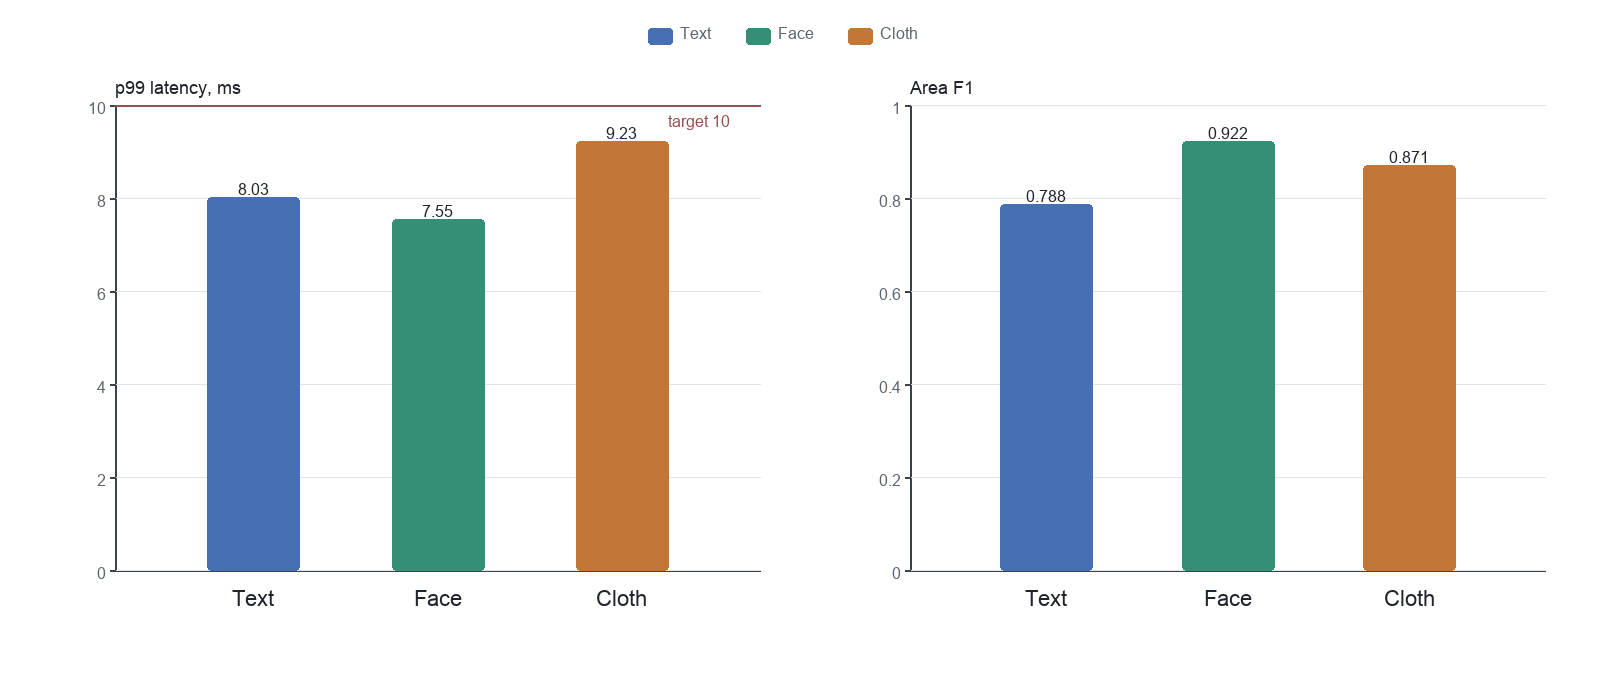
\includegraphics[width=0.92\linewidth]{performance/selected_detector_profiles.png}
  \caption{p99-задержка и Area F1 для выбранных detector-конфигураций IDet.}
  \label{fig:selected_detector_profiles}
\end{figure}

Рисунок~\ref{fig:selected_detector_profiles} показывает, что все выбранные профили остаются ниже
порога $10\,\ms$ по p99, но отличаются характером компромисса: Face имеет лучший Area F1,
Text жертвует precision ради recall, а Cloth удерживает наибольшую задержку из трех режимов.

% 7.5 Метрики и знак improvement

\section{Метрики и знак improvement}

Используются пять групп метрик. Global metrics измеряют качество всего кадра: PSNR, SSIM, VMAF,
$Q_{\mathrm{JOD}}$, LPIPS и DISTS \cite{psnr,ssim,vmaf,lpips,dists,fovvideovdp}. ROI-only
метрики считаются только внутри ROI mask. Background metrics измеряют область вне ROI.
Thesis-weighted метрики повышают вес ROI в общей оценке. ROI-crop-weighted метрики считаются по
ROI-кропам и агрегируются с учетом площади ROI.

Для PSNR, SSIM, VMAF и $Q_{\mathrm{JOD}}$ большее значение означает лучшее качество. Для
LPIPS и DISTS меньшее значение означает лучшее качество. Все improvement нормализованы так, что
положительное значение означает преимущество ROI-aware над baseline; поэтому для LPIPS и DISTS
improvement считается как baseline минус ROI-aware. $Q_{\mathrm{JOD}}$ использовался как
относительная full-reference perceptual metric (метрика с полным эталоном) при одинаковой
нормализации входных изображений для baseline и ROI-aware ветвей. В агрегированных сводках mean improvement показывает средний эффект
ROI-aware относительно baseline, median improvement --- медианный эффект, std improvement ---
разброс, а positive share --- долю положительных случаев.

% 7.6 Результаты ROI-aware кодирования

\section{Результаты ROI-aware кодирования}

Положительное значение improvement в таблицах~\ref{tab:roi_global_results}--\ref{tab:roi_crop_results}
означает преимущество ROI-aware над baseline. Отрицательное значение означает, что соответствующая
метрика снизилась относительно baseline при сопоставимом размере потока.

\begin{table}[H]
  \centering
  \caption{Средние значения improvement для global, background и thesis-weighted метрик}
  \label{tab:roi_global_results}
  \scriptsize
  \begin{tabularx}{\linewidth}{@{}l Z Z Z Z Z Z Z@{}}
    \toprule
    Mode & Global PSNR & Global VMAF & Global $Q_{\mathrm{JOD}}$ & Background PSNR & Background SSIM & Weighted PSNR & Weighted SSIM \\
    \midrule
    Text & -0.206 & -0.305 & -0.044 & -0.382 & -0.0019 & 0.059 & -0.0002 \\
    Face & -0.115 & -0.226 & -0.021 & -0.204 & -0.0013 & 0.021 & 0.0004 \\
    Cloth & -0.138 & -0.115 & -0.043 & -1.148 & -0.0085 & 0.080 & 0.0001 \\
    \bottomrule
  \end{tabularx}
  \par\smallskip
  {\footnotesize Background --- область вне ROI; Weighted --- thesis-weighted метрика, где ROI имеет повышенный вес. Положительное значение improvement означает преимущество ROI-aware над baseline.}
\end{table}

\begin{table}[H]
  \centering
  \caption{Средние значения improvement для ROI-only и ROI-crop-weighted метрик}
  \label{tab:roi_crop_results}
  \scriptsize
  \begin{tabularx}{\linewidth}{@{}l Z Z Z Z Z Z Z@{}}
    \toprule
    Mode & ROI PSNR & ROI SSIM & Crop PSNR & Crop VMAF & Crop $Q_{\mathrm{JOD}}$ & Crop LPIPS & Crop DISTS \\
    \midrule
    Text & 3.331 & 0.0253 & 3.028 & 4.451 & 0.166 & 0.0107 & 0.0466 \\
    Face & 3.284 & 0.0303 & 2.871 & 5.857 & 0.415 & 0.0300 & 0.0408 \\
    Cloth & 0.547 & 0.0017 & 0.971 & 0.449 & 0.034 & 0.0023 & 0.0028 \\
    \bottomrule
  \end{tabularx}
  \par\smallskip
  {\footnotesize Crop обозначает ROI-crop-weighted метрики: качество считается по кропам ROI и агрегируется с учетом их площади. Для LPIPS и DISTS знак improvement развернут, поэтому положительное значение также означает преимущество ROI-aware.}
\end{table}

\begin{table}[H]
  \centering
  \caption{Positive share для ключевых ROI-crop-weighted improvement}
  \label{tab:roi_crop_positive_share}
  \small
  \begin{tabularx}{\linewidth}{@{}l Z Z Z Z Z@{}}
    \toprule
    Mode & Crop PSNR & Crop VMAF & Crop $Q_{\mathrm{JOD}}$ & Crop LPIPS & Crop DISTS \\
    \midrule
    Text & 1.00 & 1.00 & 1.00 & 1.00 & 1.00 \\
    Face & 1.00 & 1.00 & 1.00 & 1.00 & 1.00 \\
    Cloth & 0.95 & 0.90 & 1.00 & 0.95 & 0.95 \\
    \bottomrule
  \end{tabularx}
  \par\smallskip
  {\footnotesize Positive share --- доля изображений, где ROI-aware оказался лучше baseline по соответствующей ROI-crop-weighted метрике.}
\end{table}

Таблица~\ref{tab:roi_global_results} показывает поведение всего кадра и фона. В ней отрицательные
global/background значения не являются ошибкой: при \texttt{match\_baseline} общий размер потока
остается почти неизменным, поэтому усиление ROI компенсируется более жестким
квантованием менее важных областей. Наиболее показателен Cloth: background PSNR снижается на
$1.148\,\mathrm{dB}$, но weighted PSNR остается положительным. Это означает, что перераспределение
качества попадает в целевую область, хотя глобальное усреднение по кадру частично скрывает
локальный выигрыш.

Таблица~\ref{tab:roi_crop_results} фиксирует результат там, где ROI-aware кодирование должно
проявляться сильнее всего: внутри масок ROI и на ROI-кропах. Text и Face дают крупный локальный
прирост по PSNR и VMAF, потому что текстовые области и лица компактнее, лучше согласованы с
детектором и сильнее выигрывают от дополнительного битового бюджета. Cloth также показывает
положительные значения по всем ROI-crop метрикам, но меньшей величины: это более сложная и
размытая категория, где объект часто содержит неоднородные ткани, складки, границы одежды и фон.
Таблица~\ref{tab:roi_crop_positive_share} дополняет средние значения: положительная доля близка
к единице, следовательно, эффект не сводится к нескольким удачным изображениям.

\begin{figure}[H]
  \centering
  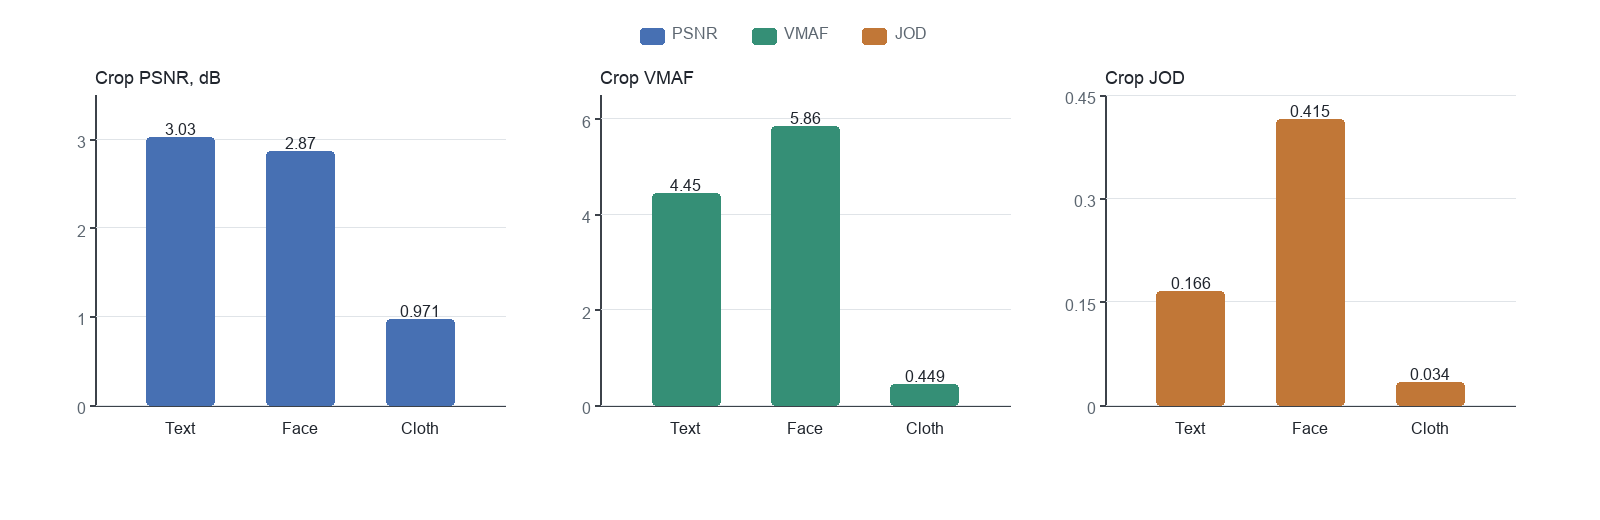
\includegraphics[width=0.92\linewidth]{video-quality/roi_crop_effects.png}
  \caption{ROI-crop-weighted improvement по PSNR, VMAF и $Q_{\mathrm{JOD}}$ для трех
      режимов.}
  \label{fig:roi_crop_effects}
\end{figure}

Рисунок~\ref{fig:roi_crop_effects} показывает главный локальный эффект: ROI-crop метрики
положительны во всех трех режимах. Самый большой ROI-crop VMAF improvement зафиксирован для
Face ($+5.857$), затем Text ($+4.451$); для Cloth эффект меньше по абсолютной величине
($+0.449$), но остается положительным и устойчивым по доле положительных случаев.

\begin{figure}[H]
  \centering
  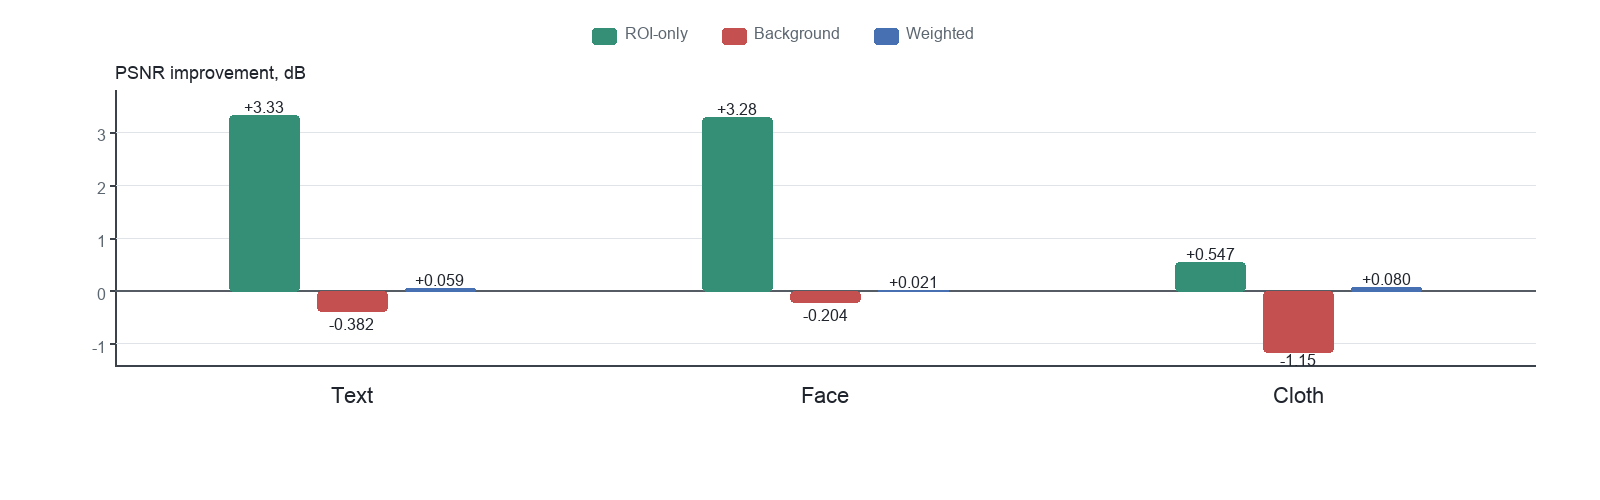
\includegraphics[width=0.92\linewidth]{video-quality/roi_background_tradeoff.png}
  \caption{Сопоставление ROI-only PSNR, background PSNR и thesis-weighted PSNR improvements.}
  \label{fig:roi_background_tradeoff}
\end{figure}

Рисунок~\ref{fig:roi_background_tradeoff} фиксирует ожидаемый компромисс режима
\texttt{match\_baseline}: ROI-only PSNR растет, background PSNR снижается, а thesis-weighted
PSNR остается положительным. Это означает перераспределение качества от фона к ROI при
сопоставимом размере потока, а не равномерное улучшение всего кадра.

% 7.7 Почему эффект ограничен

\section{Почему эффект ограничен}

Небольшая абсолютная величина части изменений не означает слабость эффекта. Эксперимент поставлен в строгом режиме \texttt{match\_baseline}: ROI-aware ветка не получает дополнительного битового бюджета, а только
перераспределяет уже имеющийся бюджет между ROI и фоном. В такой постановке крупный рост
качества внутри ROI почти неизбежно сопровождается снижением качества вне ROI. Поэтому ожидаемый
результат --- не улучшение всех метрик сразу, а положительный локальный эффект при контролируемом
компромиссе по фону.

Второй фактор --- выбранный baseline. В работе использован не искусственно слабый baseline, а
фиксированная HEVC-конфигурация на \texttt{libx265} с preset \texttt{medium} и CRF 32. Такой
baseline уже умеет адаптивно распределять биты по сложным участкам кадра, поэтому ROI-aware слой
соревнуется не с примитивным кодированием, а с сильным кодировщиком. Это делает прирост более
честным: результат показывает добавленную ценность ROI side data сверх стандартной rate-control
логики HEVC.

Третий фактор --- консервативная политика \texttt{qoffset}. В работе не подбирался максимально
агрессивный \texttt{qoffset}, который мог бы искусственно завысить локальный эффект ценой
деградации фона. Напротив, параметры выбраны так, чтобы не приводить к чрезмерной деградации фона и сохранять
сопоставимый размер потока. Для Text и Face смещение сильнее, потому что эти области компактны и
субъективно важны. Для Cloth используется более мягкая защита: эта настройка дает меньший
численный выигрыш, но лучше соответствует производственной логике, где текстурированные ROI
имеют меньший приоритет, чем текст и лица.

Разница между Cloth и режимами Text/Face объясняется также природой самих областей. Текст и лица
имеют более устойчивую семантическую структуру: небольшое повышение качества в буквах, контурах
лица и деталях глаз быстро отражается в ROI-crop метриках. Одежда и фактуры распределены иначе:
они занимают большую и менее однородную площадь, содержат высокочастотные детали, складки,
границы с фоном и участки разной важности. Кроме того, прямоугольная ROI для одежды чаще
захватывает лишнюю площадь, поэтому часть выделенного бюджета уходит не только на действительно
значимые фактуры. Поэтому меньший эффект Cloth является ожидаемым свойством более сложного
режима, а не признаком неработоспособности подхода.

Именно поэтому основной вывод по эксперименту формулируется не как «ROI-aware улучшает
весь кадр», а как «ROI-aware стабильно улучшает области интереса при сопоставимом размере
потока». Метод демонстрирует управляемое перераспределение качества в пользу областей интереса
на фиксированной HEVC-конфигурации и при ограниченном бюджете, а дальнейший рост эффекта может достигаться отдельным
подбором \texttt{qoffset}, приоритетов ROI и видеоспецифических temporal-механизмов.

% 7.8 Интерпретация по режимам

\section{Интерпретация по режимам}

В режиме Text ROI ветка ROI-aware кодирования дало устойчивый локальный выигрыш: ROI-only PSNR вырос на
$3.331\,\mathrm{dB}$, ROI-only SSIM --- на $0.0253$, ROI-crop VMAF --- на $4.451$, а
доля положительных случаев по ключевым ROI-crop метрикам равна $1.00$. Одновременно global VMAF
снизился на $0.305$, background PSNR --- на $0.382\,\mathrm{dB}$. Такой результат соответствует
цели: текстовые области защищены лучше, а часть битового бюджета снята с фона.

Для Face ROI локальный эффект также устойчив: ROI-only PSNR вырос на $3.284\,\mathrm{dB}$,
ROI-only SSIM --- на $0.0303$, ROI-crop VMAF --- на $5.857$,
ROI-crop $Q_{\mathrm{JOD}}$ --- на $0.415$. Глобальные метрики при этом немного снизились:
global PSNR на $0.115\,\mathrm{dB}$, global VMAF на $0.226$. Это согласуется с режимом \texttt{match\_baseline}: локальная защита лиц достигается за счет перераспределения битов, а не за
счет роста общего размера потока.

Для Cloth ROI глобальные метрики слегка снижаются: global PSNR на $0.138\,\mathrm{dB}$,
global SSIM на $0.0008$, global VMAF на $0.115$, global $Q_{\mathrm{JOD}}$ на $0.043$. При этом
ROI-only и ROI-crop-weighted метрики демонстрируют положительный эффект: ROI-only PSNR
$+0.547\,\mathrm{dB}$, ROI-crop PSNR $+0.971\,\mathrm{dB}$, ROI-crop VMAF $+0.449$,
ROI-crop $Q_{\mathrm{JOD}}$ $+0.034$. Background PSNR снижается на $1.148\,\mathrm{dB}$, а
background SSIM на $0.0085$; это является прямым следствием приоритизации областей одежды и
фактур при сопоставимом размере потока.

% 7.9 Выводы по главе

\section{Выводы по главе}

Покадровая схема сравнения baseline и ROI-aware на основе \texttt{FFmpeg addroi} и \texttt{libx265}
реализован и проверен для трех режимов IDet: Text, Face и Cloth. Для всех режимов использован
CRF baseline 32, preset \texttt{medium} и режим \texttt{match\_baseline}; средний
\texttt{size\_ratio} находится около 1.0, поэтому сравнение выполнено при сопоставимом размере
потока.

Эксперимент подтверждает локальный эффект ROI side data: ROI-only и ROI-crop-weighted метрики
улучшаются во всех трех режимах. Ухудшение background и части global metrics не противоречит
цели метода, потому что при фиксированном битовом бюджете кодировщик перераспределяет качество
от фона к ROI. Полученный результат подтверждает применимость ROI side data для приоритизации
значимых областей. Полноценное сравнение на видеопотоке требует отдельного этапа с
пространственно-временным сглаживанием, tracking ROI, GOP-структурой и оценкой сетевой доставки,
поэтому в данной работе оно вынесено за границы эксперимента.

% ==============================================================================
%           8. Экспериментальное исследование производительности IDet
% ==============================================================================

\chapter{Экспериментальное исследование производительности IDet}

% 8.1 Назначение benchmark-эксперимента

\section{Назначение benchmark-эксперимента}

Экспериментальное исследование производительности IDet направлено на проверку того, может ли
ROI-детекция использоваться в CPU-first видеоконвейере без нарушения целевого бюджета задержки.
В отличие от главы, посвященной обучению YOLO-модели, здесь оценивается не качество отдельного
ML-checkpoint, а поведение runtime-конфигураций IDet: задержка обработки кадра, устойчивость
хвоста распределения, качество геометрического покрытия ROI и стоимость разных режимов разбиения
изображения на плитки.

Для оценки использовались grid-search эксперименты по трем режимам библиотеки:
\begin{enumerate}[label=\arabic*)]
  \item \important{text ROI} --- детекция текстовых областей;
  \item \important{face ROI} --- детекция лиц;
  \item \important{textured ROI} --- детекция одежды и фактурных областей.
\end{enumerate}

Каждая конфигурация характеризуется набором runtime-параметров: размером входа модели, схемой
разбиения на плитки, числом потоков ONNX Runtime, числом потоков tiled-обработки и режимом I/O
Binding. Для каждой точки фиксировались значения $p50$, $p90$, $p95$ и $p99$ задержки, а также
area-based proxy качества относительно reference-прогона: $\operatorname{AreaRecall}$,
$\operatorname{AreaPrecision}$, $\operatorname{AreaF_1}$ и $\operatorname{ExtraAreaRatio}$,
определенные ранее в разделе о метриках покрытия ROI.

Важно подчеркнуть, что reference-прогон в данном эксперименте не является ручной ground
truth-разметкой. Он используется как инженерный proxy: более дорогая или более консервативная
конфигурация задает ожидаемую область покрытия, а быстрые варианты сравниваются с ней по площади
пересечения. Такой подход позволяет оценивать компромисс между скоростью и сохранением
ROI-геометрии без необходимости вручную размечать каждый benchmark-кадр.

% 8.2 Дисциплина измерения задержки

\section{Дисциплина измерения задержки}

Для корректного измерения latency важно отделять чистый benchmark от диагностических запусков. В
чистом режиме отключались отрисовка, сохранение результатов и подробный вывод:
\begin{center}
  \texttt{--is\_draw 0 --is\_dump 0 --verbose 0}.
\end{center}
Именно этот режим использовался для измерения $p50/p90/p95/p99$. Отдельный короткий запуск с
\texttt{--is\_dump 1} применялся только для выгрузки ROI-геометрии и расчета area-based метрик.
Эти два режима нельзя смешивать: dump и диагностический вывод добавляют I/O-операции, которые
искажают задержку hot path.

Время внешнего Python-скрипта, запускающего grid search, не трактуется как latency IDet. Оно
может сохраняться как служебное поле, но финальные выводы о скорости должны строиться по
значениям, которые печатает сам \texttt{idet\_app}. Такой подход исключает влияние
\texttt{subprocess}, парсинга stdout и файловых операций на измерение производительности
runtime-слоя.

Для real-time сценария ключевым является не среднее значение, а хвост распределения. Средняя
задержка может быть приемлемой, но редкие пики приводят к пропуску deadline кадра, накоплению
очереди или необходимости отключать часть детекторов. Поэтому в данной работе основной метрикой
выбора runtime-конфигурации является $p99$, а $p50$ используется как характеристика типичного
поведения.

Измерения производительности IDet выполнялись не на обучающей GPU-станции, а на сервере с двумя
сокетами Kunpeng 920B, 224 GB RAM и двумя 48-ядерными ARM CPU. Итого сервер предоставляет
96 физических CPU-ядер, однако benchmark в этой работе намеренно не использует всю машину как
единый вычислительный ресурс. Цель эксперимента --- найти рабочие точки, пригодные для
производственного видеоконвейера, где часть ядер должна оставаться доступной кодировщику,
сетевому вводу-выводу и другим сервисным задачам.

По этой причине измерения трактуются как проверка конфигураций в заданном CPU-бюджете, а не как
поиск абсолютного максимума скорости на сервере. Для двухсокетной NUMA-системы это особенно
важно: выход за пределы локальной группы ядер может дать больше параллелизма, но одновременно
увеличить межсокетные обращения к памяти и шум в хвосте задержки.

% 8.3 Рабочие точки IDet

\section{Рабочие точки IDet}

По результатам grid-search эксперимента для дальнейшего ROI-aware кодирования выбрана одна
основная рабочая точка на режим. Эти точки уже использованы в главе~7 и приведены в
таблице~\ref{tab:roi_selected_detectors}. Здесь они рассматриваются с позиции производительности:
выбор выполнялся не по одному минимальному $p99$, а по компромиссу между задержкой, recall,
precision, Area F1 и лишней защищаемой площадью.

В grid-search скрипте была задана верхняя граница в 32 потока на конфигурацию. Это не предел
сервера Kunpeng 920B: на тестовой машине доступно 96 CPU-ядер. Ограничение в 32 потока выбрано
как инженерный бюджет для одной ROI-ветки: оно остается внутри локального 48-ядерного сокета,
снижает риск NUMA-штрафов и оставляет запас для видеокодировщика. Поэтому значения в
таблице~\ref{tab:roi_selected_detectors} следует читать как лучшие найденные рабочие точки внутри
заданного бюджета, а не как абсолютный потолок производительности оборудования.

Выбранный Text ROI профиль использует сетку $5\times6$, вход $64\times128$,
\texttt{threads\_intra}=2 и \texttt{tile\_omp}=30. Он задействует весь заданный бюджет
32 потоков и дает $p99=8.032\,\ms$ при Area F1 $0.788$. Для текста это оправдано: recall
$0.886$ важнее минимального p99, потому что пропущенный текст не получает защиты в кодировщике.

Для Face ROI используется сетка $3\times4$, вход $128\times192$, \texttt{threads\_intra}=8 и
\texttt{tile\_omp}=12. Профиль дает $p99=7.553\,\ms$, Area Recall $0.916$, Area Precision
$0.929$ и Area F1 $0.922$. Он лучше соответствует задаче качества, чем ultra-speed варианты с
меньшим покрытием лиц, и остается ниже целевого бюджета $10\,\ms$.

Для Cloth ROI используется сетка $2\times4$, вход $128\times128$, \texttt{threads\_intra}=8 и
\texttt{tile\_omp}=8. Профиль дает $p99=9.230\,\ms$, Area Recall $0.920$ и Area F1 $0.871$.
Extra Area Ratio $0.192$ является приемлемым для текстурированных областей: небольшое расширение
ROI дешевле, чем пропуск одежды или фактур, которые затем не смогут получить повышенный
приоритет в кодировщике.

% 8.4 Latency-quality trade-off

\section{Компромисс между задержкой и качеством покрытия}

На рисунке~\ref{fig:bench_latency_quality} каждая точка соответствует одной конфигурации grid
search. По оси задержки используется $p99$, поскольку именно эта метрика отражает риск нарушения
deadline кадра. По оси качества используется $\operatorname{AreaF_1}$, объединяющая полноту
покрытия reference ROI и аккуратность candidate ROI.

\begin{figure}[!htbp]
  \centering
  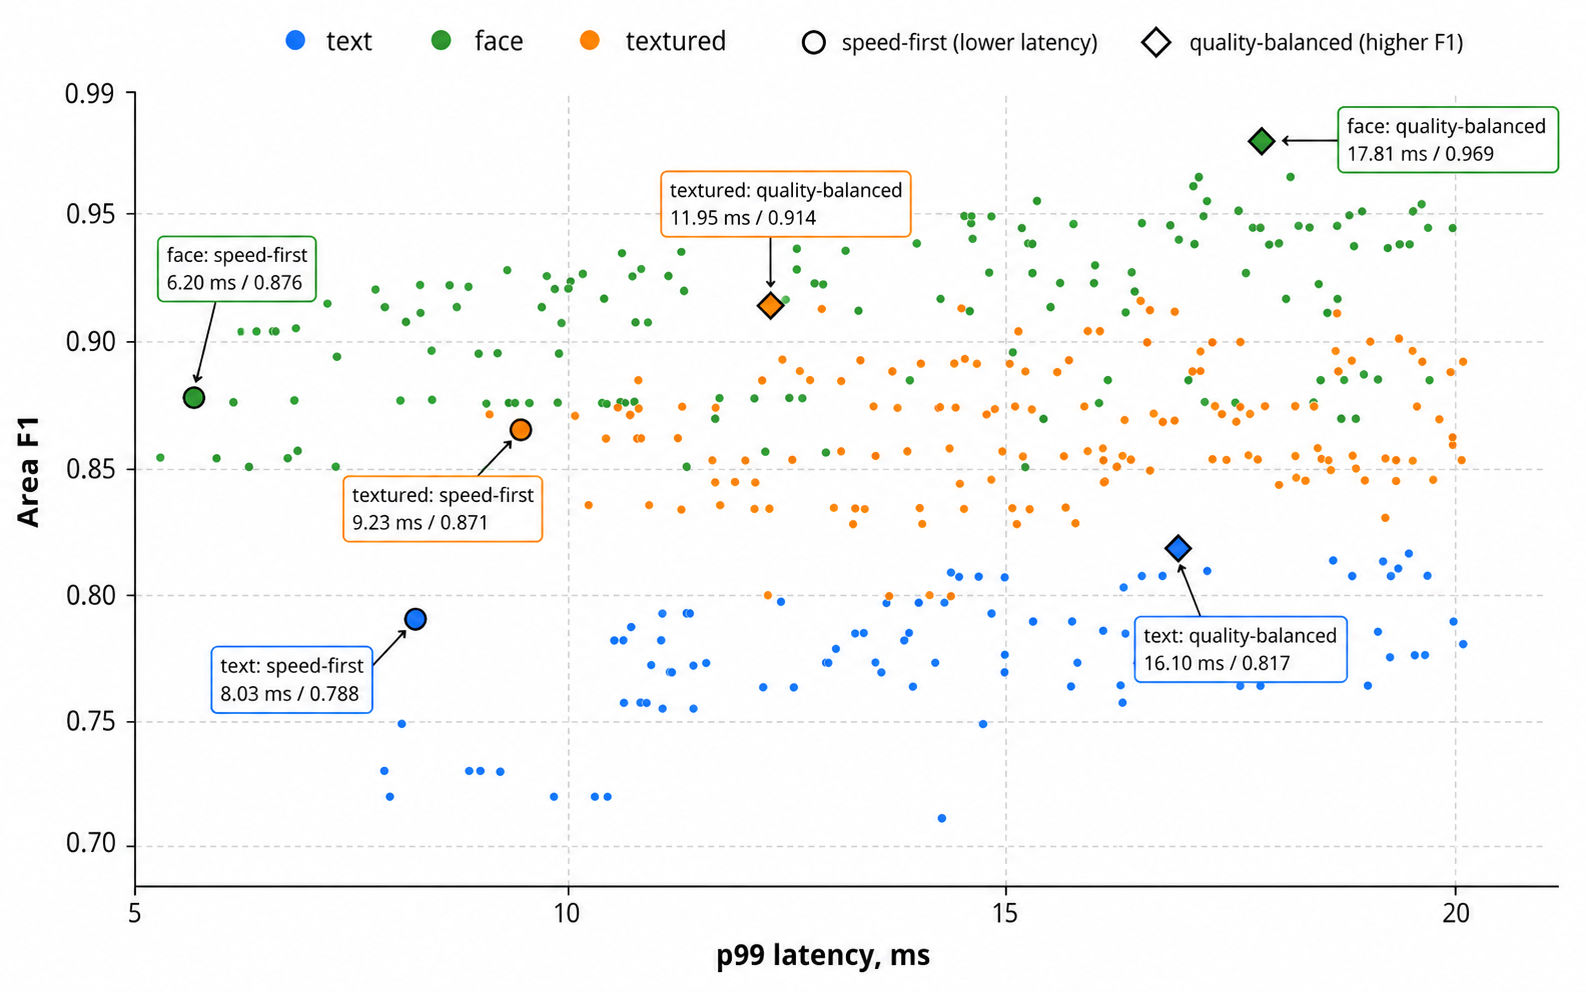
\includegraphics[width=0.90\linewidth]{performance/p99_area_f1_tradeoff.png}
  \caption{Компромисс между p99-задержкой и Area F1 для текстового режима, режима лиц и режима
      текстурированных ROI в IDet.}
  \label{fig:bench_latency_quality}
\end{figure}

Рисунок~\ref{fig:bench_latency_quality} показывает, что универсальной настройки IDet нет.
Для Text ROI повышение покрытия достигается за счет более агрессивного tiling и большего
плиточного параллелизма. Для Face ROI выбранная точка находится в balanced-области: она не
минимизирует p99 любой ценой, но дает более надежное покрытие лиц. Для Cloth ROI выбранный
профиль находится у границы целевого бюджета $10\,\ms$ и сохраняет достаточно высокий recall.

Tiled inference может снижать задержку отдельного кадра, но эффект зависит от модели и схемы
плиток. Слишком мелкое разбиение увеличивает overhead stitching и NMS, а слишком крупные плитки
уменьшают выигрыш от параллелизма. Поэтому параметры \texttt{tiles\_rc}, \texttt{fixed\_hw} и
\texttt{tile\_omp} должны подбираться совместно.

% 8.5 Интерпретация по режимам

\section{Интерпретация по режимам}

Text ROI использует наиболее высокий бюджет потоков CPU среди выбранных профилей. Это
соответствует характеру задачи: текст часто занимает малую площадь, поэтому важнее не потерять
область, чем добиться максимальной точности границ. Для последующего кодирования такая стратегия
повышает шанс защитить все читаемые фрагменты.

Face ROI показывает самый высокий Area F1 среди выбранных точек. Это важно для субъективного
качества: заметные артефакты на лице воспринимаются сильнее, чем такие же артефакты в фоне.
Выбранная рабочая точка сохраняет баланс между качеством покрытия и p99, не уходя в дорогие
quality-first конфигурации.

Cloth ROI работает ближе всего к верхней границе latency budget. Это ожидаемо для
текстурированных областей: модель YOLO и постобработка одежды тяжелее, чем выбранная
SCRFD-конфигурация для детекции лиц. Тем не менее выбранная точка укладывается в $10\,\ms$ и
затем в главе~7 дает положительный ROI-crop эффект при кодировании.

% 8.6 I/O Binding и локальность памяти

\section{I/O Binding и локальность памяти}

I/O Binding в ONNX Runtime позволяет заранее связать входные и выходные тензоры с конкретными
буферами и уменьшить лишние перемещения данных между этапами исполнения \cite{ort_iobinding}. В
CPU-only сценарии это особенно важно для tail latency: непредсказуемые копирования и неудачная
локальность памяти могут ухудшать $p95/p99$ даже при приемлемом среднем времени.

Профилирование использовалось как диагностический инструмент. Сравнивались режимы с включенным и
выключенным I/O Binding при зафиксированном состоянии NUMA balancing. В
таблице~\ref{tab:memory_locality} показано, что I/O Binding существенно повышает долю локального
memory traffic. Например, для textured tiled доля локальных обращений выросла с $48.01\%$ до
$94.31\%$, для face tiled --- с $55.49\%$ до $94.88\%$, для text tiled --- с $48.73\%$ до
$91.43\%$.

\begin{table}[!htbp]
  \centering
  \caption{Влияние I/O Binding на локальность памяти}
  \label{tab:memory_locality}
  \small
  \begin{tabularx}{\linewidth}{@{}l Z Z Z Z Z@{}}
    \toprule
    \multirow{2}{*}{Режим} &
    \multicolumn{3}{c}{Доля локального memory traffic, \%} &
    \multicolumn{2}{c}{Общий memory traffic, GB} \\
    \cmidrule(lr){2-4}
    \cmidrule(l){5-6}
    & С binding & Без binding & Прирост, п.п. & С binding & Без binding \\
    \midrule
    Textured single & 77.22 & 41.01 & 36.21 & 15.82 & 35.75 \\
    Textured tiled  & 94.31 & 48.01 & 46.30 & 35.56 & 45.68 \\
    Face single     & 84.63 & 56.47 & 28.16 & 9.41  & 14.40 \\
    Face tiled      & 94.88 & 55.49 & 39.39 & 22.93 & 20.77 \\
    Text single     & 52.35 & 44.87 & 7.48  & 31.72 & 40.24 \\
    Text tiled      & 91.43 & 48.73 & 42.70 & 23.65 & 25.94 \\
    \bottomrule
  \end{tabularx}
\end{table}

\begin{figure}[!htbp]
  \centering
  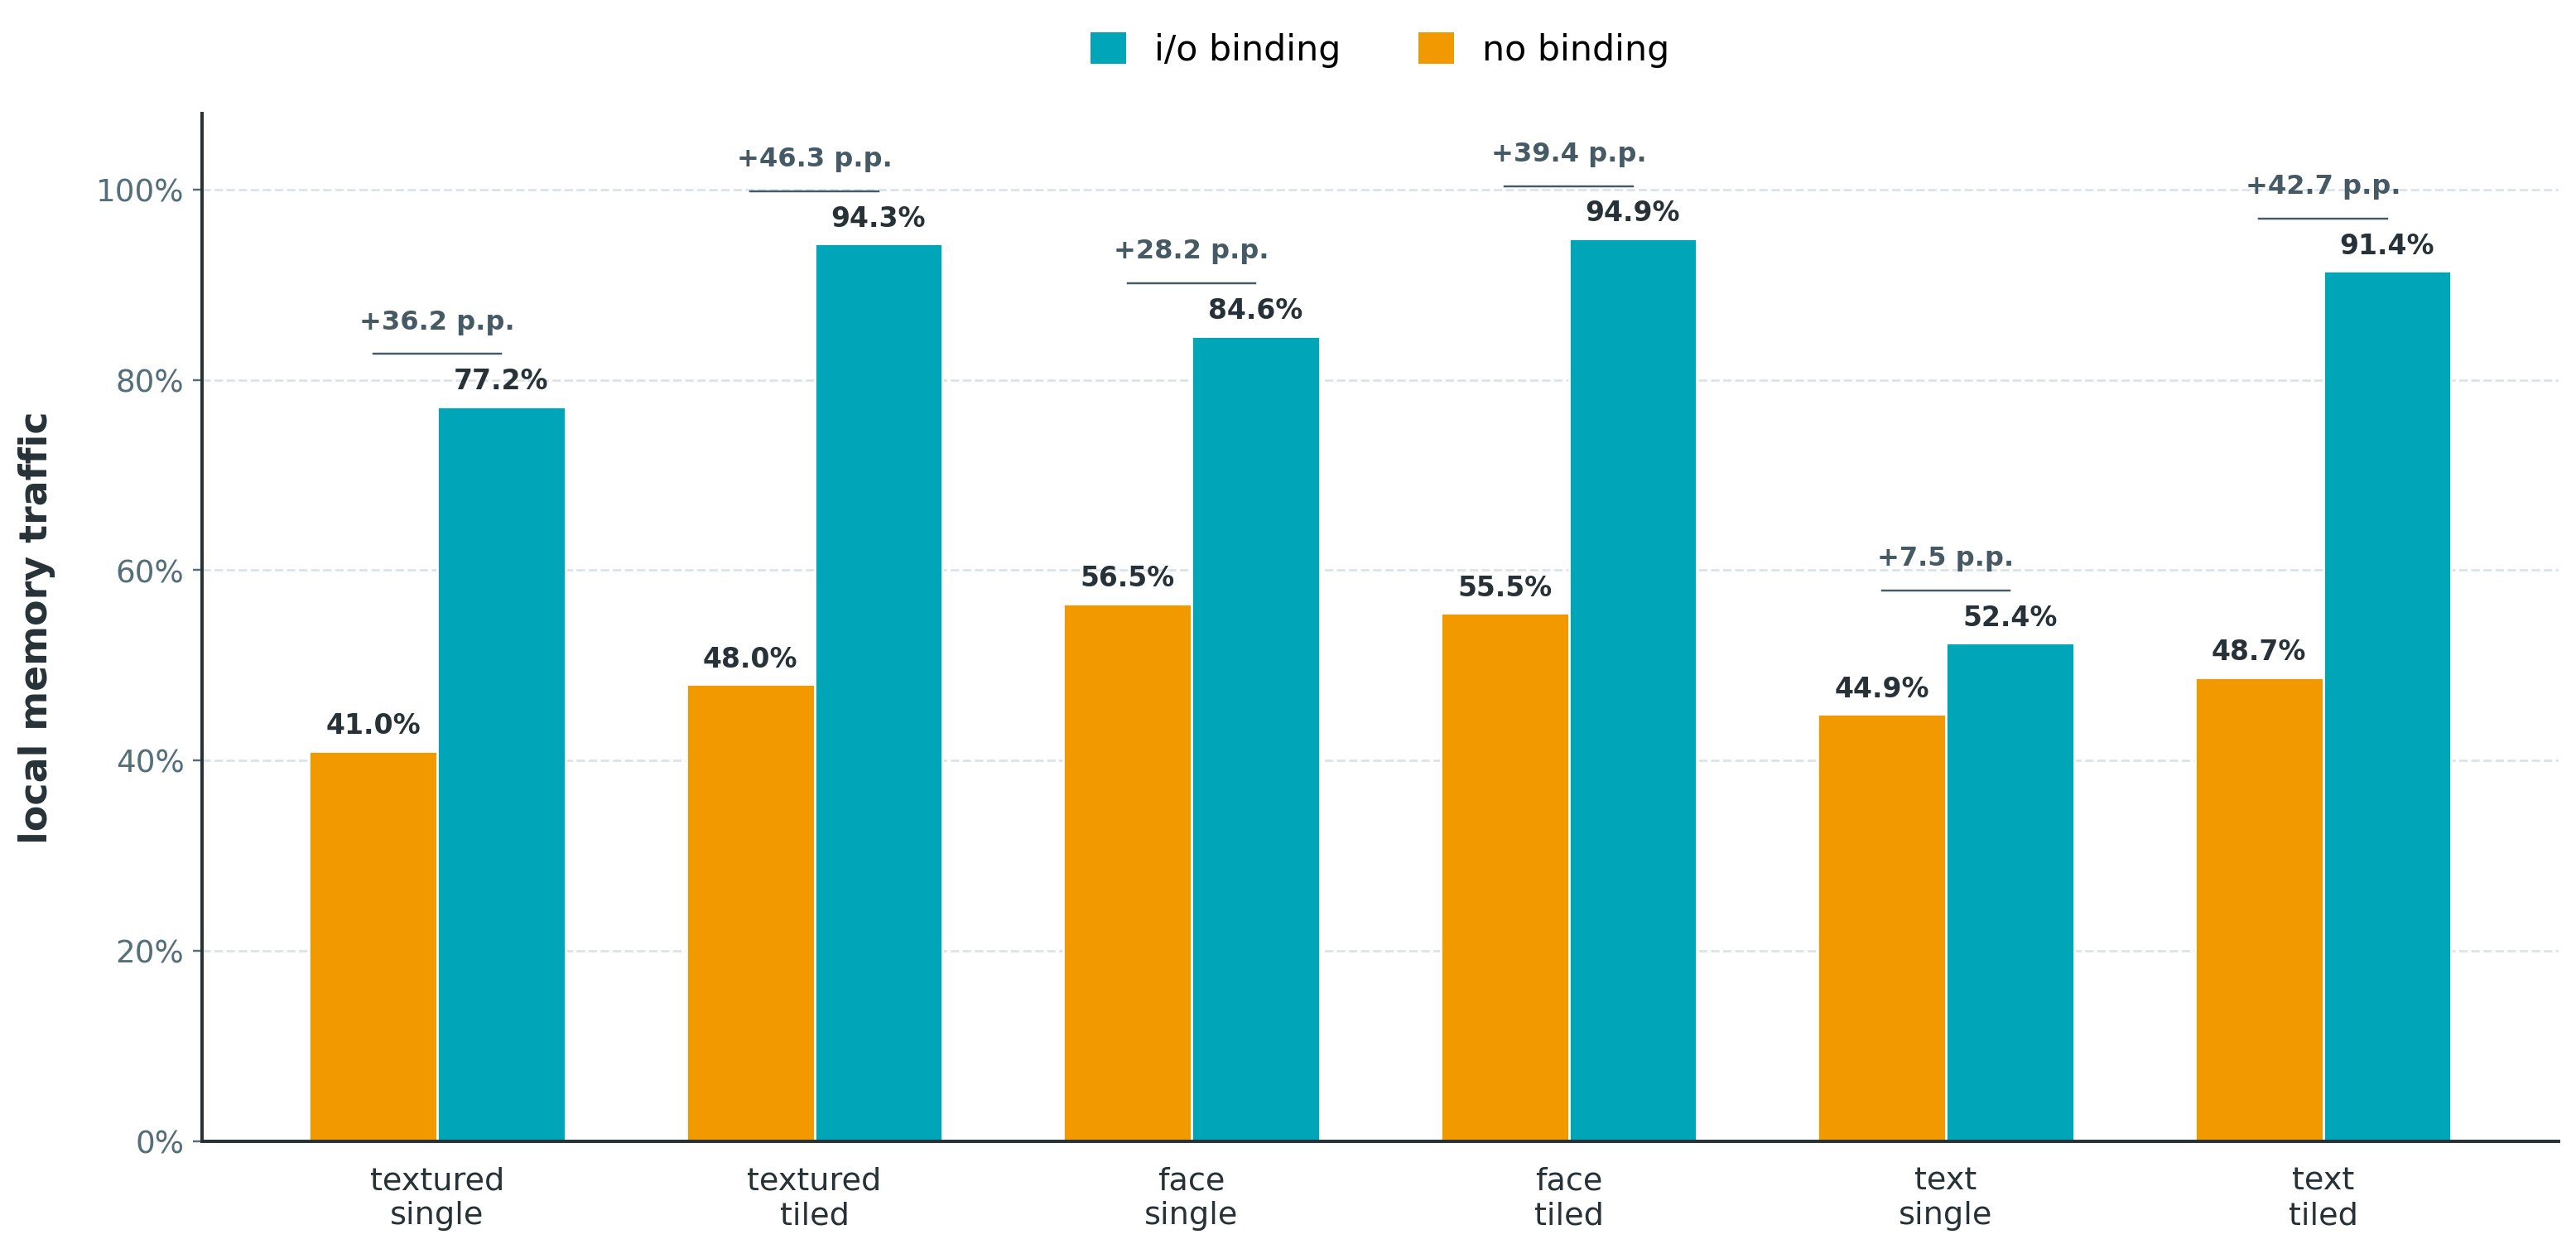
\includegraphics[width=0.90\linewidth]{profiling/io_binding_memory_locality.png}
  \caption{Доля локального memory traffic при включенном и выключенном I/O Binding.}
  \label{fig:memory_locality}
\end{figure}

Рисунок~\ref{fig:memory_locality} подтверждает главный эффект I/O Binding: он повышает
локальность обращений, но не гарантирует меньший общий объем memory traffic. Например, для
tiled-режима лиц общий трафик с I/O Binding выше, чем без него. Для закрепленных CPU-измерений
и NUMA-систем решающим является не сам объем трафика, а снижение зависимости от межузловых
обращений, которое делает хвост задержки более управляемым.

% 8.7 NUMA-аспекты CPU-only исполнения

\section{NUMA-аспекты CPU-only исполнения}

На серверных CPU итоговая задержка зависит не только от числа потоков, но и от размещения
потоков и памяти. Automatic NUMA balancing в Linux может быть полезен для обычных приложений, но
в закрепленных измерениях он способен добавлять шум из-за миграции страниц по page fault и
периодического сканирования памяти \cite{linux_numa_balancing}. Поэтому состояние
\texttt{kernel.numa\_balancing}, cpuset, memory binding и политика размещения потоков должны
фиксироваться в протоколе эксперимента.

Для IDet это особенно важно из-за сочетания двух уровней параллелизма: ONNX Runtime использует
собственные потоки intra-op/inter-op, а tiled-режим добавляет внешний параллелизм по плиткам.
Если оба уровня настроены слишком агрессивно, возникает переподписка потоков: несколько пулов
конкурируют за одни и те же ядра. Поэтому параметры \texttt{threads\_intra},
\texttt{threads\_inter} и \texttt{tile\_omp} должны рассматриваться как единая политика среды
выполнения.

Практический вывод состоит в том, что оптимальные настройки нельзя переносить между машинами без
повторной проверки. Конфигурация, оптимальная для одного cpuset или NUMA-узла, может стать
неоптимальной при изменении числа доступных ядер, памяти или версии ONNX Runtime. Поэтому
таблицы измерений фиксируют не только задержку и качество, но и полный набор параметров потоков.

% 8.8 Top-Down Microarchitecture Analysis

\section{Top-Down Microarchitecture Analysis}

Top-Down Microarchitecture Analysis позволяет классифицировать, как процессор расходует слоты
конвейера исполнения \cite{topdown,arm_topdown}. В этой методике:
\begin{enumerate}[label=\arabic*)]
  \item \textit{Retiring} соответствует полезно завершенным инструкциям;
  \item \textit{Frontend Bound} отражает ограничения подачи инструкций;
  \item \textit{Backend Bound} связан с ожиданием данных, памяти или исполнительных ресурсов;
  \item \textit{Bad Speculation} показывает потери из-за неверных предсказаний и сбросов конвейера
      исполнения.
\end{enumerate}

На рисунке~\ref{fig:tma_breakdown} показана реконструированная сводка для диагностических
прогонов без I/O Binding. Режимы single-shot имеют более высокую долю \textit{Retiring}:
примерно $60.65\%$ для текста, $62.77\%$ для лиц и $65.88\%$ для текстурированных ROI. В
tiled-режиме возрастает доля \textit{Backend Bound}: для текста --- до $51.94\%$, для лиц --- до
$49.47\%$, для текстурированных ROI --- до $58.60\%$.

\begin{figure}[!htbp]
  \centering
  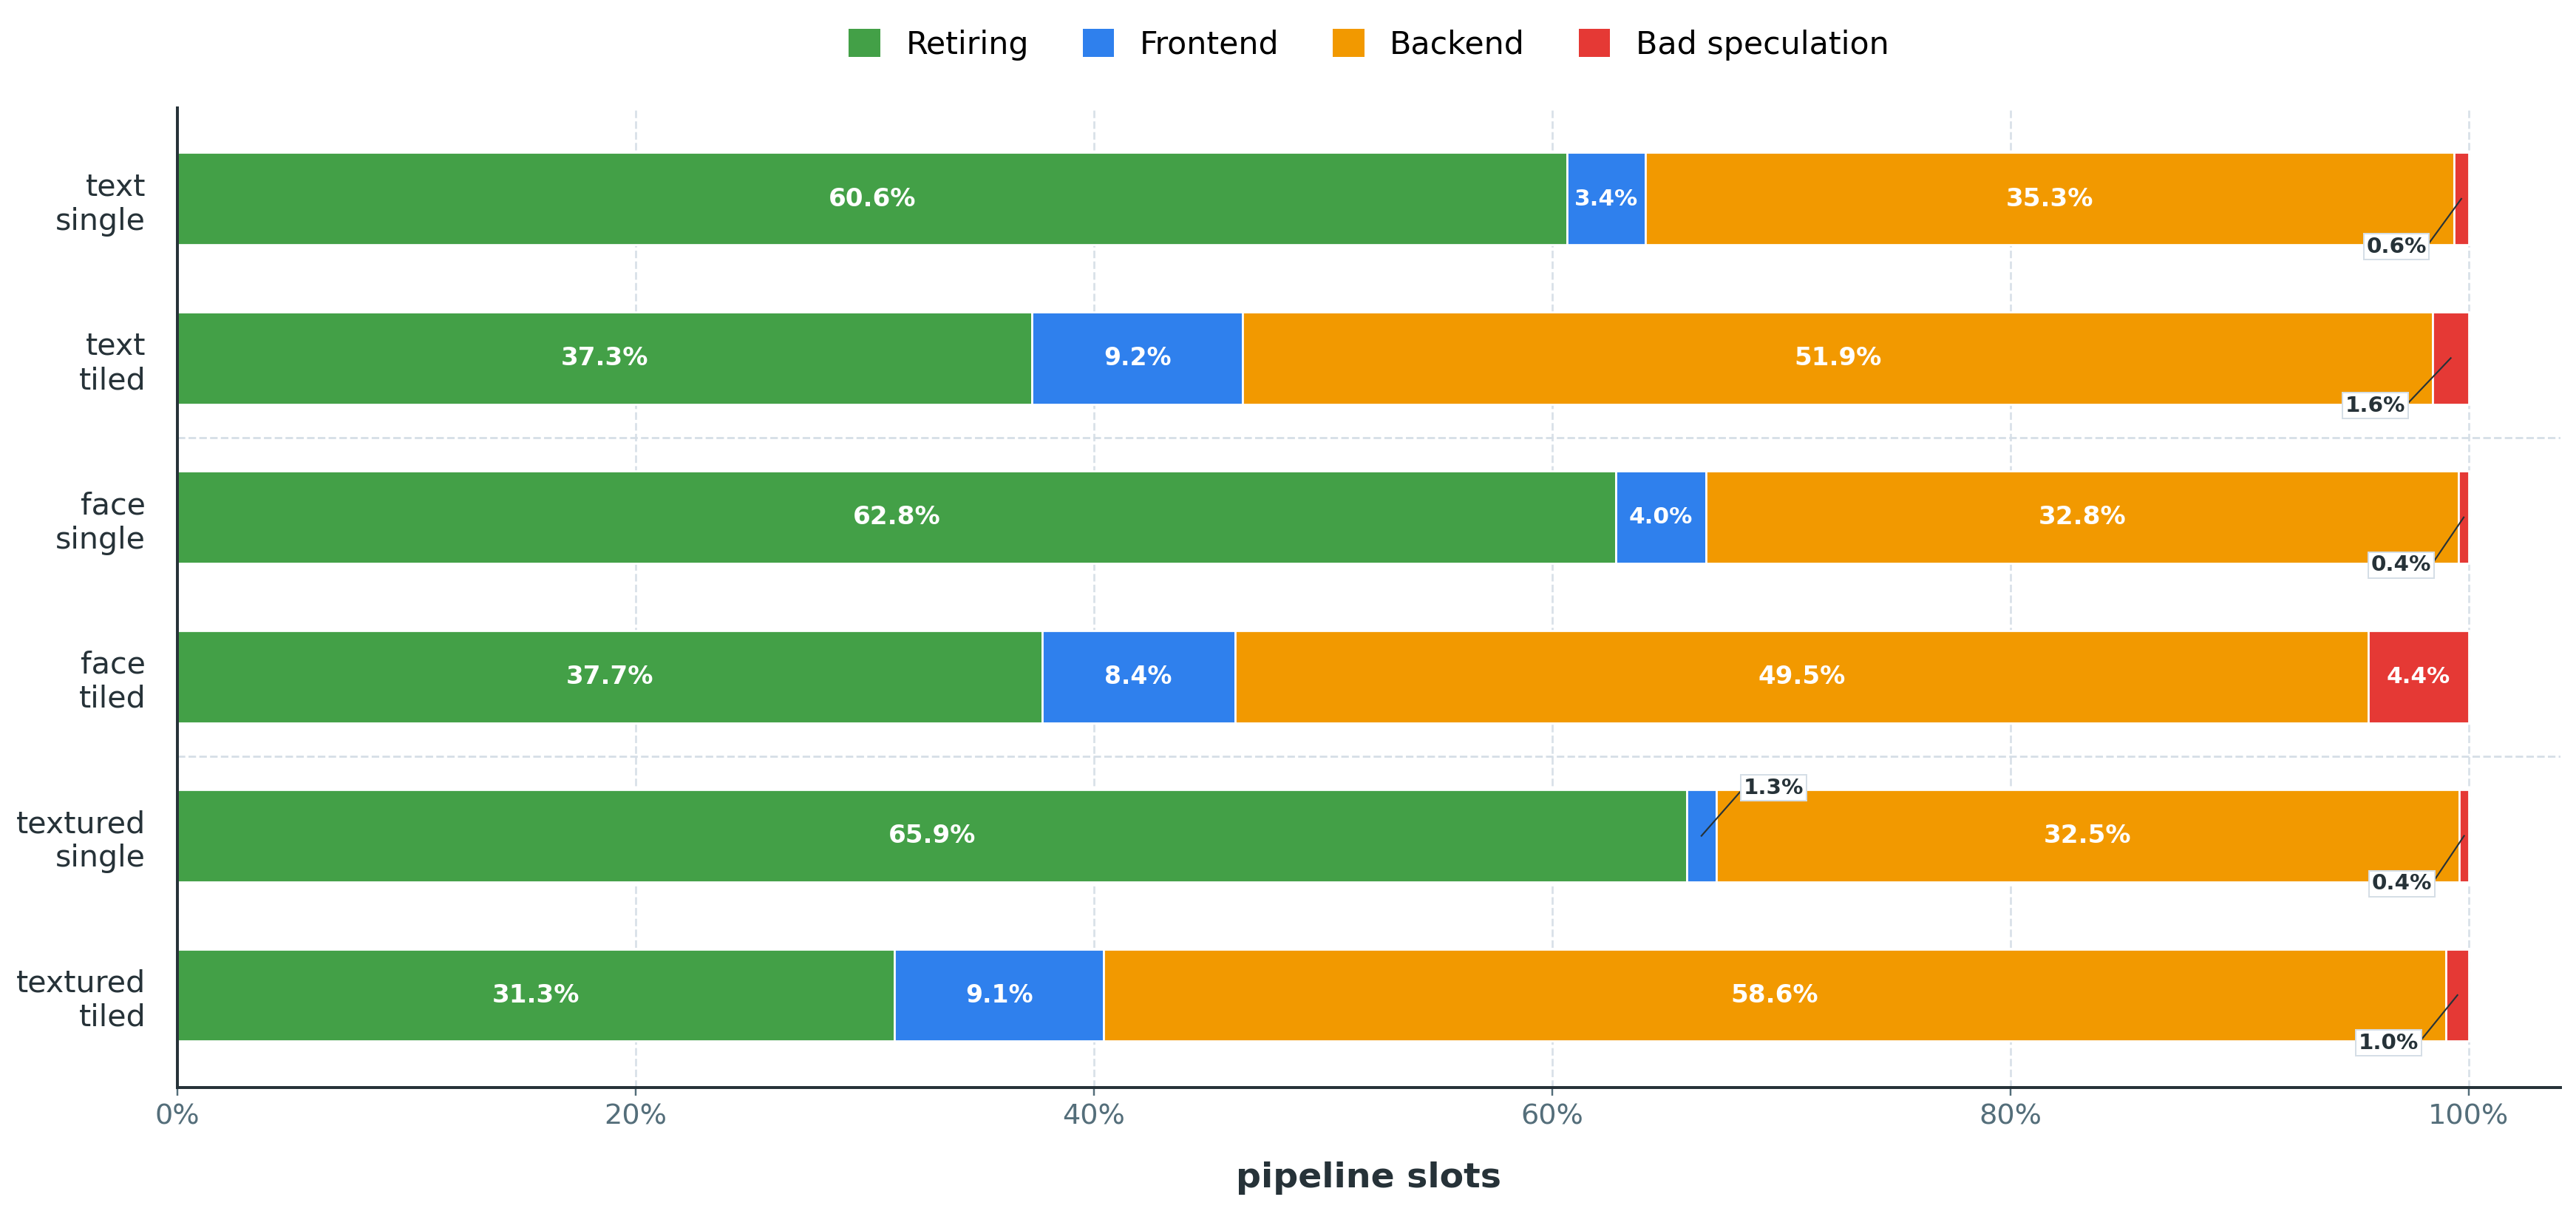
\includegraphics[width=0.95\linewidth]{profiling/tma_breakdown.png}
  \caption{Top-Down Microarchitecture Analysis для single/tiled режимов в диагностических прогонах
      без I/O Binding.}
  \label{fig:tma_breakdown}
\end{figure}

Рисунок~\ref{fig:tma_breakdown} показывает, что tiled-режимы повышают параллелизм, но чаще
становятся backend-bound. Это объясняет, почему увеличение числа плиток и потоков не всегда
улучшает p99.

Такой результат согласуется с природой tiled-инференса. Разбиение на плитки повышает параллелизм
и позволяет лучше использовать CPU, но одновременно увеличивает давление на память,
синхронизацию, планирование среды выполнения и постобработку. Поэтому рост параллелизма не
гарантирует автоматического снижения $p99$: конфигурация может стать backend-bound и упереться
не в арифметику, а в доступ к данным.

Дополнительно tiled-режимы увеличивают долю NEON SIMD-инструкций. Для текстовых ROI она
возрастает примерно с $10$--$14\%$ до $40\%$, для ROI лиц --- примерно с $9$--$14\%$ до
$33$--$34\%$, для текстурированных ROI --- примерно с $6$--$8\%$ до $36$--$37\%$. Это
показывает, что tiled-инференс действительно активнее использует SIMD-вычисления, но итоговый
выбор конфигурации все равно должен основываться на $p99$ и качестве покрытия одновременно.

\begin{figure}[!htbp]
  \centering
  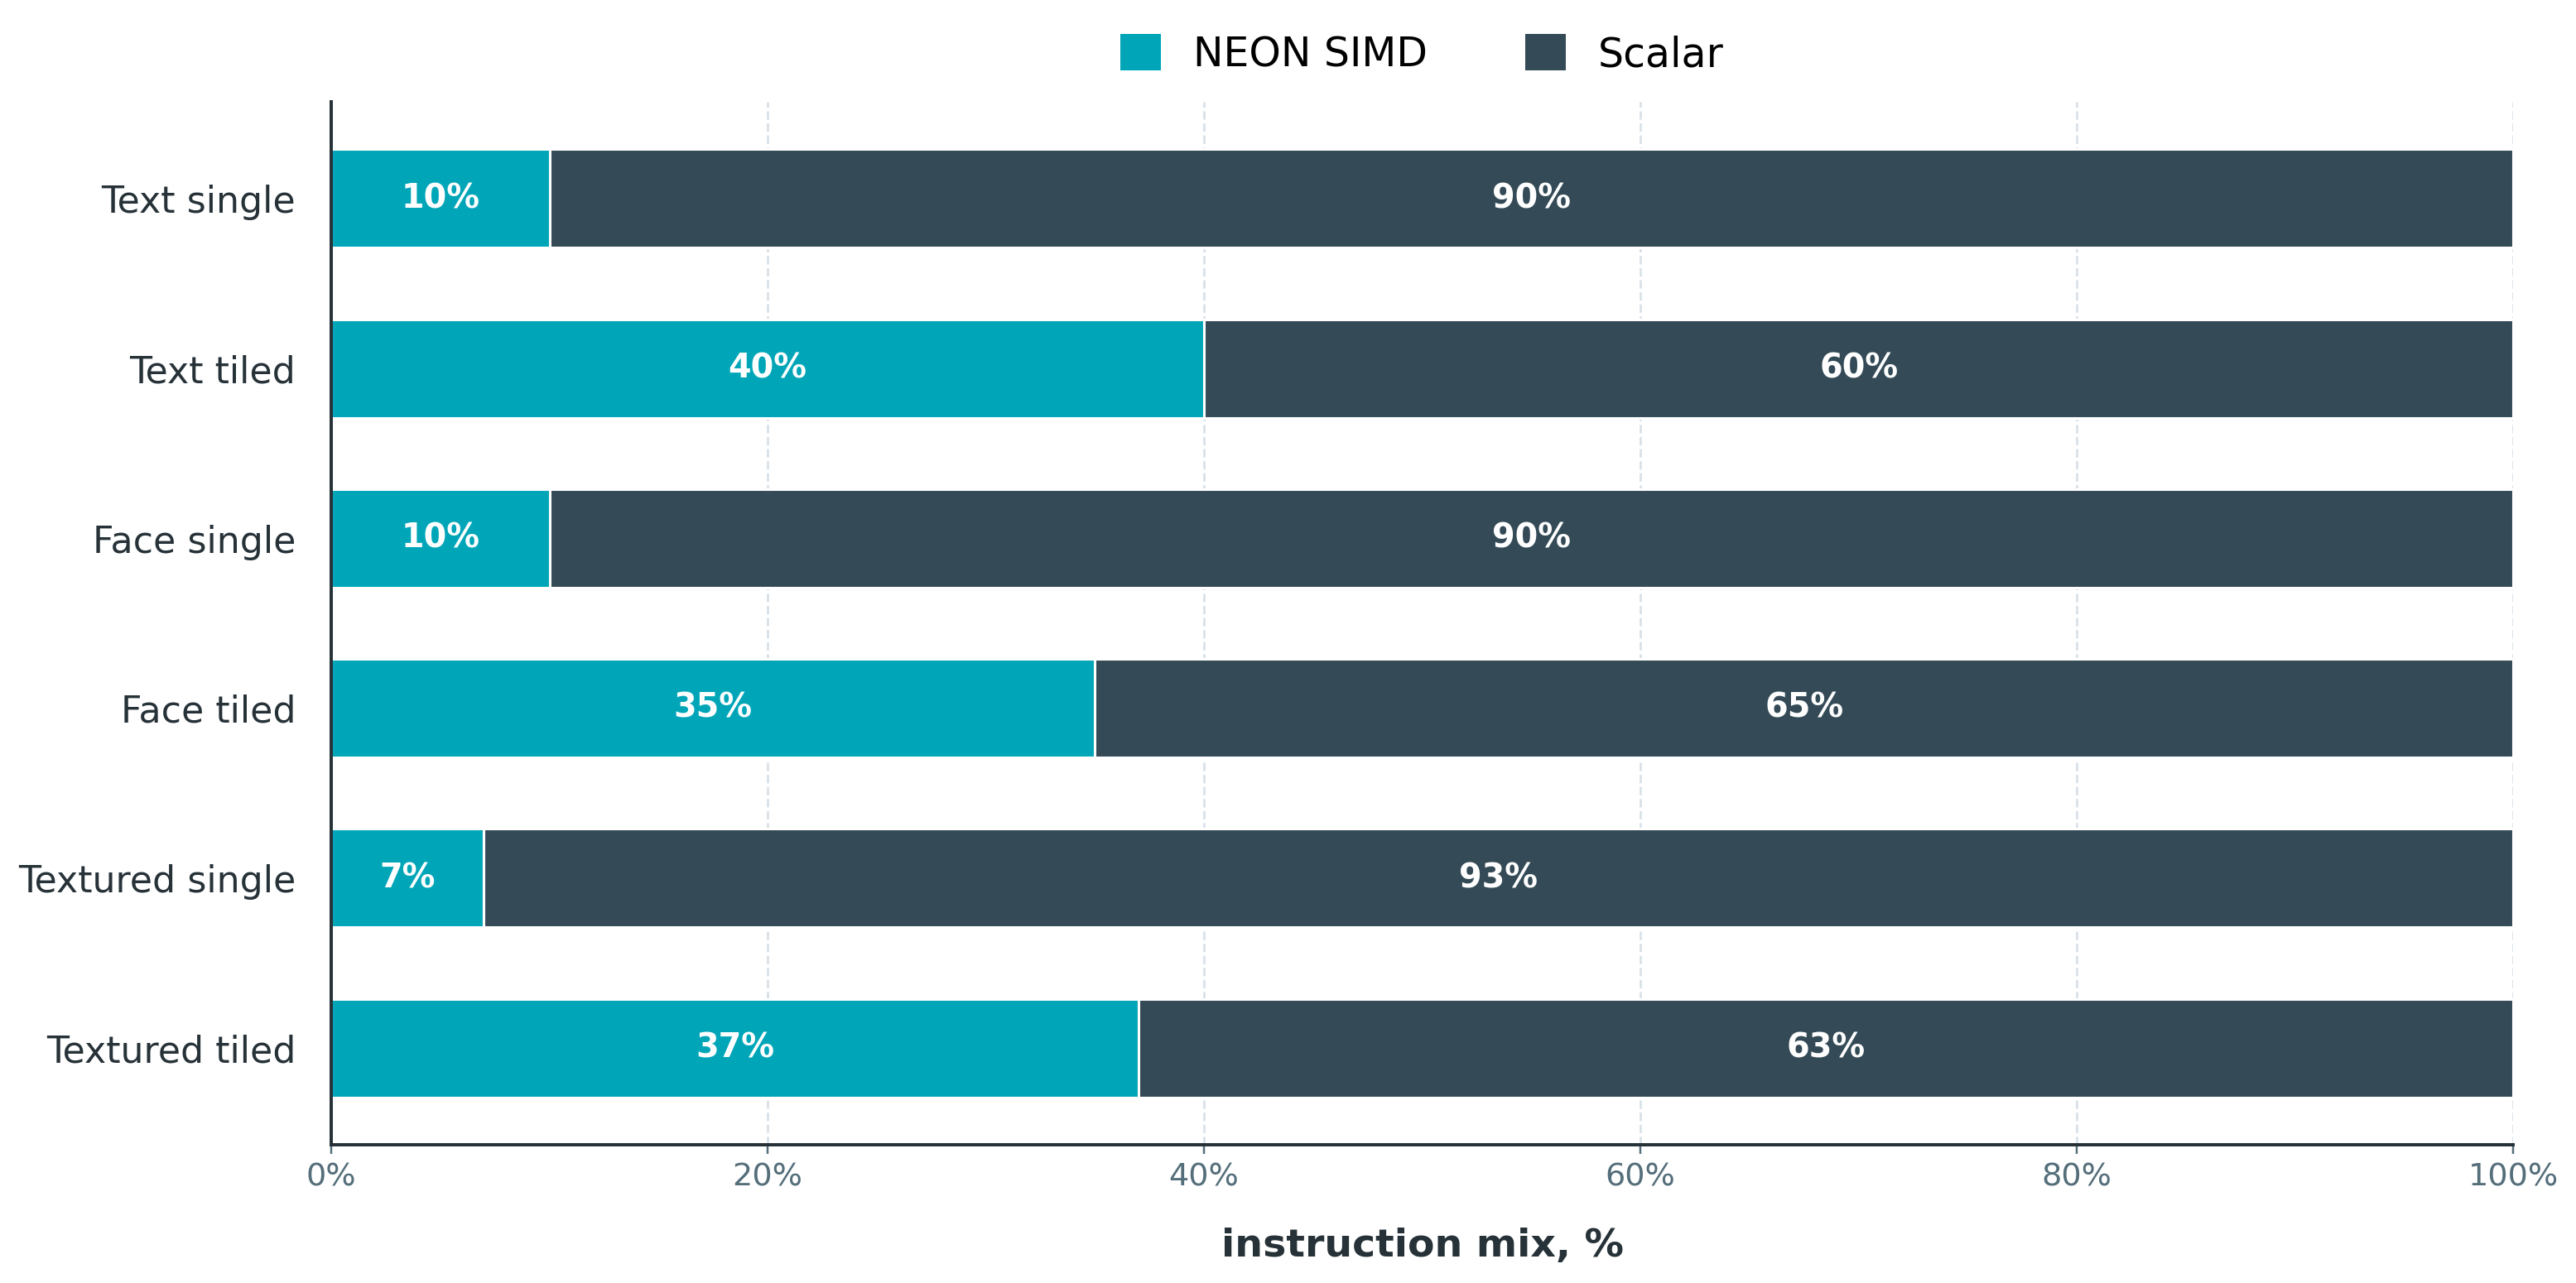
\includegraphics[width=0.82\linewidth]{profiling/neon_simd_share.png}
  \caption{Доля NEON SIMD-инструкций в single и tiled режимах.}
  \label{fig:neon_mix}
\end{figure}

Рисунок~\ref{fig:neon_mix} подтверждает, что tiled inference активнее нагружает векторные
вычисления, но выбирать конфигурацию только по SIMD-доле нельзя: решающими остаются p99 и
качество покрытия.

Для углубленного анализа hotspot-ов может использоваться Linux perf, предоставляющий sampling и
hardware performance counters \cite{linux_perf}. На ARM-системах дополнительно может применяться
Statistical Profiling Extension, если она доступна в конкретной аппаратной и системной
конфигурации \cite{arm_spe}. Если профилировщик сообщает о недоступности SPE, это не является
ошибкой IDet, но ограничивает глубину микроархитектурного анализа.

% 8.9 Ограничения текущих benchmark-данных

\section{Ограничения текущих benchmark-данных}

Полученные таблицы измерений подтверждают пригодность отдельных режимов IDet к развертыванию, но
относятся именно к слою ROI-детекции. У этих данных есть несколько ограничений.

Во-первых, метрики покрытия по площади сравнивают ROI-кандидаты с референсным прогоном, а не с
ручной разметкой видео. Поэтому они показывают согласованность быстрых конфигураций с выбранным
референсом, но не измеряют абсолютную семантическую правильность ROI.

Во-вторых, измерения выполнялись на отдельных изображениях. Видеопоследовательность добавляет
межкадровые эффекты: размытие движения, изменение масштаба, частичное перекрытие объектов,
нестабильность детектора и необходимость временного сглаживания. Поэтому результаты на
изображениях должны быть дополнены прогоном на видеокорпусе.

В-третьих, задержка в этой главе относится к слою ROI-детекции. Она не включает полный
видеокодировщик, расчет VMAF/SSIM, передачу метаданных ROI в бэкенд кодировщика и возможные
накладные расходы интеграционного слоя. Поэтому результаты этой главы подтверждают, что IDet
формирует ROI в реалистичном CPU-бюджете, а качество после кодирования оценивается отдельно в
покадровом эксперименте главы~7.

% 8.10 Выводы по главе

\section{Выводы по главе}

Экспериментальное исследование показывает, что IDet имеет практические рабочие конфигурации для
всех трех режимов ROI. Текстовые ROI достигают $p99=8.032\,\ms$, ROI лиц --- $p99=7.553\,\ms$,
текстурированные ROI --- $p99=9.230\,\ms$. Эти значения относятся к отдельным веткам ROI-детекции
и не означают, что все три детектора должны запускаться последовательно на каждом кадре в рамках
того же бюджета. Полный трехрежимный видеоконвейер требует планировщика запусков, переноса ROI
между кадрами и отдельного end-to-end измерения.

Выбор рабочих точек отражает разную цену ошибок. Text ROI делает акцент на recall, Face ROI
дает наилучший Area F1 среди выбранных профилей, а Cloth ROI сохраняет высокий recall/F1 при
задержке ниже $10\,\ms$. Эти профили далее использованы в покадровом сравнении кодирования.

I/O Binding существенно повышает локальность памяти в NUMA-сценарии, особенно для tiled-режимов.
Top-Down Microarchitecture Analysis показывает, что tiled-инференс активнее использует SIMD, но
одновременно может становиться backend-bound. Поэтому оптимизация IDet должна учитывать не
только время инференса модели, но и весь критический путь: предобработку, планирование среды
выполнения, локальность памяти, постобработку, NMS, сшивание плиток и слияние ROI.

Главный практический вывод главы состоит в следующем: IDet нельзя настраивать одной
универсальной конфигурацией. Для производственной интеграции нужны профили политики среды
выполнения: скоростной профиль для live-сценариев, сбалансированный профиль качества для
nearline/offline обработки и адаптивное планирование для полного трехрежимного конвейера.

% ==============================================================================
%      9. Производственная интеграция, ограничения и план развития IDet
% ==============================================================================

\chapter{Производственная интеграция, ограничения и план развития IDet}

% 9.1 Граница производственной интеграции

\section{Граница производственной интеграции}

Результаты предыдущих глав показывают, что IDet может формировать ROI в CPU-ориентированном
режиме и имеет рабочие точки с приемлемым $p99$ для отдельных веток текста, лиц и
текстурированных ROI. Однако производственная интеграция требует рассматривать библиотеку не как
набор независимых детекторов, а как часть видеоконвейера. В таком конвейере ROI-детекция должна
получать кадры из потока, работать в заданном бюджете задержки, возвращать стабильную геометрию
областей и не создавать непредсказуемую нагрузку на память, CPU и кодировщик.

В текущей архитектуре публичный контракт IDet остается геометрическим: библиотека возвращает
список четырехугольников \texttt{VecQuad}. Это решение упрощает API и отделяет компьютерное
зрение от политики кодирования. Производственная ROI-aware система строится поверх этого слоя:
последующий компонент добавляет тип области, приоритет, ограничение площади, временное
сглаживание и отображение в \texttt{qoffset} или другую управляющую информацию для кодировщика.
Такое разделение важно, потому что оно не привязывает IDet к конкретной версии FFmpeg, x265 или
другому бэкенду кодирования.

Следовательно, производственная интеграция IDet должна состоять из трех уровней:
\begin{enumerate}[label=\arabic*)]
  \item \important{Слой извлечения ROI} --- собственно IDet, выполняющий детекцию текста, лиц и
      текстурированных областей;
  \item \important{Слой управления ROI} --- слияние областей, приоритизация, ограничение площади и
      стабилизация во времени;
  \item \important{Слой интеграции с кодировщиком} --- преобразование метаданных ROI в
      \texttt{qoffset}, ROI side data или резервную политику.
\end{enumerate}

Такой подход позволяет развивать систему поэтапно. На первом этапе достаточно стабильно получать
ROI и измерять их качество. На втором этапе можно использовать ROI для offline-анализа качества.
На третьем этапе ROI подключаются к кодировщику и проверяются сначала покадрово, как в главе~7,
а затем на полноценном видеопотоке с учетом temporal mechanisms.

% 9.2 Режимы эксплуатации

\section{Режимы эксплуатации}

Предлагаемая система может использоваться в нескольких режимах эксплуатации. Они отличаются
жесткостью требований к задержке и способом использования ROI.

\begin{table}[!htbp]
  \centering
  \caption{Режимы эксплуатации ROI-aware системы на базе IDet}
  \label{tab:deployment_modes}
  \small
  \begin{tabularx}{\linewidth}{@{}P{0.22\linewidth}P{0.25\linewidth}Y@{}}
    \toprule
    Режим & Основная цель & Особенности использования ROI \\
    \midrule
    Offline-анализ &
    Анализ качества и подготовка отчетов. &
    ROI используются для расчета локальных метрик, визуального сравнения и подбора политики
      кодирования. Жесткого бюджета задержки нет. \\
    Assisted encoding &
    Улучшение VoD или nearline-транскодирования. &
    ROI передаются кодировщику, но допускается более высокая задержка. Можно использовать
      сбалансированные профили качества. \\
    Real-time streaming &
    Live или интерактивный видеопоток. &
    ROI должны формироваться в жестком бюджете задержки. Нужны скоростные профили, периодический
      запуск детекторов, временное переиспользование и строгое ограничение площади. \\
    \bottomrule
  \end{tabularx}
\end{table}

Для данной ВКР наиболее важен сценарий реального или близкого к реальному времени, потому что
именно он задает основные инженерные ограничения. Однако offline-анализ и assisted encoding
также полезны: они позволяют проверить корректность ROI, подобрать \texttt{qoffset}-политику и
провести расширенные baseline vs ROI-aware эксперименты без риска нарушить live-конвейер.

% 9.3 Runtime-профили

\section{Профили среды выполнения}

Результаты главы с измерениями показывают, что универсальной конфигурации IDet для всех
сценариев нет. Поэтому производственная система должна поддерживать несколько профилей среды
выполнения.

\begin{table}[!htbp]
  \centering
  \caption{Предлагаемые профили среды выполнения IDet}
  \label{tab:runtime_profiles}
  \small
  \begin{tabularx}{\linewidth}{@{}P{0.20\linewidth}P{0.25\linewidth}Y@{}}
    \toprule
    Профиль & Цель & Характеристика \\
    \midrule
    Speed-first &
    Минимизировать $p99$ задержку. &
    Использует быстрые tiled-конфигурации, ограничивает размер входа и число кандидатов,
      допускает умеренное снижение Area F1. \\
    Quality-balanced &
    Повысить качество покрытия ROI. &
    Использует более дорогие конфигурации с лучшими Area Recall/Area F1, подходит для nearline
      или режима периодического запуска. \\
    Adaptive &
    Подстраиваться под состояние потока. &
    Меняет частоту запуска детекторов, переносит ROI между кадрами, отключает тяжелые ветки при
      росте задержки. \\
    Diagnostic &
    Собирать отладочные данные. &
    Разрешает выгрузку ROI, подробный вывод и дополнительные метрики, но не используется для
      чистого измерения задержки. \\
    \bottomrule
  \end{tabularx}
\end{table}

Speed-first профиль подходит для live-сценариев, где важнее предсказуемость задержки.
Quality-balanced профиль полезен для проверки максимального качества ROI и для offline/nearline
кодирования. Adaptive профиль является наиболее перспективным для полной трехрежимной системы:
он позволяет запускать дорогие детекторы не на каждом кадре, а между запусками использовать
временное сглаживание и перенос областей.

% 9.4 Планировщик трех режимов ROI

\section{Планировщик трех режимов ROI}

Последовательный запуск детекторов текста, лиц и текстур на каждом кадре может превысить целевой
бюджет задержки. Поэтому производственная версия IDet должна использовать планировщик режимов.
Его задача --- решать, какие детекторы запускать на текущем кадре, какие ROI можно
переиспользовать с предыдущих кадров, а какие области необходимо обновить немедленно.

Простейшая политика может быть задана следующим образом:
\begin{enumerate}[label=\arabic*)]
  \item текстовые ROI запускаются чаще в сценариях с субтитрами, интерфейсом или презентациями;
  \item ROI лиц запускаются чаще в talking-head и video conference сценариях;
  \item текстурированные ROI запускаются реже, если одежда и крупные объекты стабильны во времени;
  \item при превышении бюджета задержки тяжелые ветки временно отключаются;
  \item ROI с высокой временной стабильностью переносятся на несколько кадров вперед;
  \item при резкой смене сцены все ROI пересчитываются заново.
\end{enumerate}

Такой планировщик превращает IDet из статической цепочки моделей в адаптивный компонент среды
выполнения. Это особенно важно для текстурированных ROI: фактура одежды обычно меняется
медленнее, чем текстовые overlay-элементы или положение лица, поэтому нет необходимости
пересчитывать ее на каждом кадре в live-режиме.

% 9.5 Инварианты production-конвейера

\section{Инварианты production-конвейера}

Для надежной интеграции IDet в видеокодирование необходимо зафиксировать инварианты, которые
должны выполняться независимо от выбранной модели и профиля среды выполнения.

\begin{enumerate}[label=\arabic*)]
  \item координаты всех ROI должны находиться внутри границ исходного кадра;
  \item суммарная площадь защищаемых областей не должна превышать заданный бюджет площади
      $\alpha$;
  \item пересекающиеся ROI должны разрешаться по приоритету: текст $>$ лицо $>$ текстурированная
      область $>$ фон;
  \item отсутствие ROI не должно считаться ошибкой конвейера;
  \item сбой одного детектора не должен останавливать весь видеоконвейер;
  \item адаптер кодировщика должен иметь резервный путь, если нативные метаданные ROI недоступны;
  \item диагностические режимы не должны использоваться для финального измерения задержки;
  \item параметры потоков и NUMA-состояние должны фиксироваться в протоколе измерений.
\end{enumerate}

Эти инварианты отделяют исследовательский прототип от компонента, пригодного для практического
встраивания. В дипломной работе они важны как часть инженерного результата: система должна быть
не только точной на валидационном разбиении, но и предсказуемой при встраивании в реальный
конвейер.

% 9.6 Ограничения текущей реализации и данных

\section{Ограничения текущей реализации и данных}

Несмотря на высокие метрики YOLO26n и успешные CPU-only измерения отдельных режимов, текущие
результаты имеют ограничения.

Первое ограничение связано со смещением домена. DeepFashion2 и Fashionpedia состоят из
fashion-изображений, тогда как реальный видеостриминг содержит размытие движения, шум
веб-камеры, предварительное сжатие, неполные фигуры, нестандартное освещение, несколько людей в
кадре и сильные изменения масштаба. Поэтому модель текстурированных ROI должна дополнительно
проверяться на видеокорпусе, близком к целевым сценариям: лекции, видеоконференции, обзоры
товаров, talking-head и фрагменты прямых трансляций.

Второе ограничение связано с прямоугольной геометрией ROI. \texttt{Bbox} удобен для кодировщика
и дешев в обработке, но может включать фон вокруг объекта. Если текстурированная ROI слишком
широкая, часть битов будет потрачена на второстепенные области. Поэтому для текстурированных ROI
особенно важны $\operatorname{AreaPrecision}$, $\operatorname{ExtraAreaRatio}$ и отсечение в
последующем ROI-слое.

Третье ограничение связано с тем, что покадровый эксперимент не проверяет временную
стабильность. Для видео важно не только качество ROI на одном кадре, но и отсутствие мерцания
между кадрами. Поэтому перенос результата на live-видеопоток требует временных метрик:
стабильности координат, устойчивости присутствия ROI, частоты исчезновения областей и влияния
сглаживания.

Четвертое ограничение связано с отсутствием полноценного сравнения на видеопотоке. Такой этап
выходит за рамки работы, потому что требует не только повторного кодирования последовательностей,
но и реализации пространственно-временного сглаживания ROI, tracking между кадрами, настройки
GOP-структуры, контроля межкадрового предсказания и отдельной оценки доставки. Это уже
самостоятельная инженерная задача с заметными вычислительными и временными затратами.

% 9.7 Риски ложных ROI

\section{Риски ложных ROI}

Ошибки ROI-детекции имеют разную цену в зависимости от типа области. Для текстовых ROI опасен
пропуск текста: пользователь сразу замечает потерю читаемости. Для ROI лиц опасны и пропуски, и
сильные искажения геометрии, потому что артефакты лица субъективно заметны. Для текстурированных
ROI основной риск иной: модель может выделить визуально сложный фон, мебель, ковер или шумную
поверхность и тем самым потратить битовый бюджет на область, которая не является приоритетной.

Поэтому текстурированные ROI должны иметь меньший приоритет, чем текст и лица, а также жестко
ограничиваться по площади. Если текстурированная ROI пересекается с текстовой ROI или ROI лица,
приоритет должен отдаваться более важной области. Если текстурированная ROI занимает слишком
большую часть кадра, последующий слой должен уменьшить \texttt{qoffset}, обрезать область или
исключить часть кандидатов.

Для производственной политики важен не только порог уверенности, но и сочетание трех факторов:
\begin{enumerate}[label=\arabic*)]
  \item уверенность детектора;
  \item доля площади кадра;
  \item тип ROI и его приоритет для пользователя.
\end{enumerate}

Такой подход лучше соответствует видеокодированию, чем простое применение object detection
threshold. В задаче кодировщика модель не обязана идеально классифицировать одежду; она должна
формировать полезные области для перераспределения качества.

% 9.8 Практическая значимость работы

\section{Практическая значимость работы}

Практическая значимость работы состоит в том, что предложенная архитектура может быть развита до
полноценного ROI extraction layer для облачного видеостриминга. В рамках работы уже сформированы
основные элементы такой системы:
\begin{enumerate}[label=\arabic*)]
  \item CPU-ориентированная C++ библиотека IDet с единым геометрическим контрактом
      \texttt{VecQuad};
  \item трехрежимная архитектура ROI: текст, лица и текстурированные области;
  \item воспроизводимый конвейер YOLO для подготовки, аудита, обучения и экспорта модели;
  \item согласованная 7-классовая таксономия DeepFashion2 и Fashionpedia;
  \item обученная легкая YOLO26n-модель для текстурированных ROI;
  \item контракт развертывания PT-to-ONNX для переноса модели в ONNX Runtime;
  \item CPU-only измерения с анализом $p50/p95/p99$ и качества покрытия по площади;
  \item покадровый pipeline baseline vs ROI-aware на базе \texttt{FFmpeg addroi} и
      \texttt{libx265};
  \item численная оценка ROI-aware эффекта при сопоставимом размере потока.
\end{enumerate}

Таким образом, результат работы находится на стыке машинного обучения и системной инженерии.
Модель текстурированных ROI не рассматривается как самостоятельный fashion-детектор; ее
назначение --- стать частью управляемого видеоконвейера, где качество детекции, задержка, память
и влияние на кодировщик оцениваются совместно.

% 9.9 План дальнейшего развития

\section{План дальнейшего развития}

Дальнейшее развитие работы целесообразно выполнять в несколько этапов.

\begin{enumerate}[label=\arabic*)]
  \item \important{Видео-корпус для проверки смещения домена.} Необходимо собрать небольшой набор
      видеофрагментов из целевых сценариев: лекции, видеоконференции, обзоры товаров,
      talking-head и прямые трансляции.
  \item \important{Временное сглаживание.} Следует реализовать перенос ROI между кадрами,
      сглаживание уверенности и контроль мерцания.
  \item \important{Адаптивный планировщик.} Нужно добавить политику запуска детекторов с разной
      частотой в зависимости от сцены, нагрузки и бюджета задержки.
  \item \important{Адаптер кодировщика.} Необходимо реализовать практический путь передачи ROI в
      кодировщик через нативные метаданные ROI или резервную политику.
  \item \important{Видеоэксперимент baseline и ROI-aware.} Следует расширить покадровый результат
      до видеопотока с фиксированными preset, GOP, fps и temporal mechanisms.
  \item \important{Варианты INT8/ORT.} Нужно отдельно проверить FP32, QDQ INT8, QOperator INT8 и
      целевые ORT-артефакты по качеству и p99 задержке.
  \item \important{Расширение телеметрии.} Желательно фиксировать не только задержку, но и площадь
      ROI, число областей, стабильность во времени и влияние на отклонение битрейта.
\end{enumerate}

Этот план позволяет последовательно перейти от текущей исследовательско-инженерной версии к
ROI-aware системе, пригодной для практического развертывания. При этом каждый этап имеет
проверяемый критерий успеха: корректность ROI, стабильность во времени, соблюдение бюджета
задержки, совместимость с кодировщиком и подтвержденный ROI-выигрыш при сопоставимом размере
потока.

% 9.10 Выводы по главе

\section{Выводы по главе}

Производственная интеграция IDet требует рассматривать библиотеку не как отдельный детектор, а
как часть видеокодировочного конвейера. Для этого необходимо разделить ROI extraction, ROI
management и encoder integration. Такое разделение сохраняет простой публичный контракт IDet и
позволяет менять кодировщик, qoffset-политику и fallback-режимы без изменения детекторов.

Основные риски связаны со смещением домена, временной нестабильностью ROI, ложными
текстурированными ROI и возможным превышением бюджета задержки при одновременном запуске всех
режимов. Эти риски не отменяют предложенный подход, но задают требования к дальнейшей
реализации: адаптивный планировщик, временное сглаживание, ограничение площади и строгие
CPU-only измерения.

Практическая ценность работы состоит в том, что она формирует воспроизводимый путь от ML-модели
к системному ROI-aware компоненту: от подготовки датасетов и обучения YOLO26n до развертывания
через ONNX Runtime, CPU-only измерений и покадровой проверки ROI side data на реальном
кодировщике.

% ==============================================================================
%                               Заключение
% ==============================================================================

\chapter*{Заключение}
\addcontentsline{toc}{chapter}{Заключение}

В выпускной квалификационной работе рассмотрена задача повышения воспринимаемого качества
облачного видеостриминга в условиях ограниченных вычислительных ресурсов. Основная идея работы
состоит в использовании ROI-aware подхода: значимые области кадра выделяются до этапа
кодирования, после чего последующий интеграционный слой может передать кодировщику информацию о
приоритете этих областей. Такой подход дополняет классические механизмы адаптивного стриминга и
видеокодирования пространственным уровнем оптимизации: качество перераспределяется не только
между сегментами видео, но и внутри отдельного кадра.

В работе предложена архитектура трехрежимного ROI-конвейера на базе библиотеки IDet. Библиотека
рассматривается как CPU-ориентированный C++ слой между компьютерным зрением и видеокодированием.
В ее архитектуре выделены три типа областей интереса: текстовые области, лица и текстурированные
области одежды или материалов. Текстовые ROI важны для читаемости, ROI лиц --- для сохранения
субъективно значимых человеческих областей, текстурированные ROI --- для защиты визуально
богатых фактур, потеря которых воспринимается как снижение резкости и детализации.

Центральным инженерным результатом является системное описание IDet как компонента среды
выполнения. В работе зафиксированы границы ответственности библиотеки, жизненный цикл обработки
кадра, публичный геометрический контракт \texttt{VecQuad}, роль адаптеров детекторов, модель
владения буферами, политика потоков, требования к критическому пути без динамических аллокаций,
I/O Binding и NUMA-aware исполнению. Отдельно подчеркнуто, что типизация ROI, приоритеты и
\texttt{qoffset} являются последующим слоем поверх фактического публичного API IDet, а не уже
существующим публичным классом библиотеки. Это разделение предотвращает смешение реализованной
части и проектируемого слоя интеграции с кодировщиком.

Для третьего режима IDet подготовлен детектор текстурированных ROI на базе YOLO26n. Для его
обучения использован воспроизводимый конвейер обучения YOLO, включающий конвертацию DeepFashion2
и Fashionpedia в YOLO-формат, согласование таксономии до семи классов, аудит датасетов, запуск
обучения, анализ поклассовых метрик и подготовку PT-to-ONNX контракта для развертывания.
Объединенная таксономия позволила использовать преимущества обоих датасетов: масштаб
DeepFashion2 и дополнительное разнообразие Fashionpedia. При этом в работе отдельно рассмотрены
дисбаланс классов, геометрия bbox, центральное смещение объектов и ограничения переноса
fashion-датасетов на реальные видеосценарии.

Экспериментальные результаты обучения показали, что легкая модель YOLO26n достигает высокого
качества детекции на объединенной 7-классовой таксономии: precision = 0.903, recall = 0.873,
mAP@0.5 = 0.938 и mAP@0.5:0.95 = 0.818. Более тяжелая YOLO26s в отдельных экспериментах дает
прирост точности, но имеет существенно большую вычислительную стоимость: около 20.5 GFLOPs
против 5.2 GFLOPs у YOLO26n. Поэтому для CPU-ориентированной IDet выбран YOLO26n как более
практичный компромисс между качеством и задержкой.

Отдельный вклад работы состоит в формализации ROI-aware видеокодирования как ограниченной
оптимизационной задачи. Введены ограничения на задержку, вычислительный бюджет, битрейт и
суммарную площадь защищаемых областей. Рассмотрены ROI-взвешенные метрики качества, метрики
покрытия по площади, временное сглаживание, штраф за мерцание ROI и отображение приоритета ROI в
qoffset. Такой формальный слой нужен для того, чтобы работа не сводилась к обучению детектора
объектов, а описывала полную задачу перераспределения качества в видеопотоке.

В экспериментальной части по производительности проведен CPU-only grid-search для режимов
текстовых ROI, ROI лиц и текстурированных ROI. Для каждого режима выбрана рабочая точка с учетом
компромисса между задержкой и покрытием областей: Text ROI дает $p99=8.032\,\ms$ и
$\operatorname{AreaF_1}=0.788$, Face ROI --- $p99=7.553\,\ms$ и
$\operatorname{AreaF_1}=0.922$, Cloth ROI --- $p99=9.230\,\ms$ и
$\operatorname{AreaF_1}=0.871$. Эти значения подтверждают практическую применимость отдельных
веток IDet в заданном CPU-бюджете, но не являются end-to-end задержкой полного трехрежимного
видеоконвейера. Для одновременной работы всех режимов требуется планировщик, задающий частоту
запуска детекторов и правила переиспользования ROI между кадрами.

Профилирование показало, что I/O Binding существенно повышает локальность памяти в
NUMA-сценарии, особенно для режимов с разбиением кадра на плитки. Top-Down Microarchitecture
Analysis показал, что tiled inference увеличивает долю SIMD-инструкций, но одновременно может
усиливать backend-bound поведение. Поэтому оптимизация IDet должна рассматривать не только
модельный инференс, но и весь критический путь: подготовку входа, планирование ONNX Runtime,
локальность памяти, постобработку, NMS, сшивание плиток и слияние ROI.

Практическая значимость работы заключается в создании воспроизводимого пути от ML-модели к
системному ROI-aware компоненту, который повышает качество значимых областей кадра за счет
защиты ROI. В рамках работы описаны и связаны между собой: CPU-ориентированная библиотека IDet,
конвейер обучения YOLO, объединенная 7-классовая таксономия, обученная YOLO26n-модель для
текстурированных ROI, PT-to-ONNX контракт развертывания, CPU-only измерения и покадровый
pipeline baseline vs ROI-aware на базе \texttt{FFmpeg addroi} и \texttt{libx265}.

Покадровый эксперимент при CRF=32, preset \texttt{medium} и режиме \texttt{match\_baseline} был
проведен на подготовленных FHD-наборах: 3000 изображений для Text ROI, 3000 изображений для Face
ROI и 2696 изображений для Cloth ROI. Результаты показали, что ROI-aware кодирование
перераспределяет качество в пользу областей интереса при сопоставимом размере потока. Показатель ROI-crop VMAF вырос на $4.451$ в режиме Text ROI, на $5.857$ в режиме Face ROI и на $0.449$ в режиме Cloth ROI.
ROI-only PSNR также вырос во всех трех режимах: на $3.331\,\mathrm{dB}$ для Text, на
$3.284\,\mathrm{dB}$ для Face и на $0.547\,\mathrm{dB}$ для Cloth. При этом часть
global/background метрик снизилась, например background PSNR для Cloth уменьшился на
$1.148\,\mathrm{dB}$. Это не ошибка эксперимента, а ожидаемый компромисс режима \texttt{match\_baseline}: кодировщик отдает больше битов ROI и меньше фону. Меньший эффект Cloth объясняется
более мягким \texttt{qoffset}, большей неоднородностью текстурированных областей и тем, что
одежда чаще занимает широкую прямоугольную ROI с примесью фона. Поэтому основной вывод работы
состоит не в максимизации отдельной метрики, а в подтверждении управляемого локального выигрыша
на фиксированной HEVC-конфигурации без увеличения размера потока.

Основное ограничение текущих результатов состоит в покадровой постановке эксперимента. Поэтому
корректный вывод состоит не в утверждении о полном видеопотоке, а в зафиксированном frame-level
эффекте ROI side data. Сравнение на реальном видеопотоке сознательно вынесено за рамки работы:
оно требует видеокорпуса из целевых сценариев, пространственно-временного сглаживания ROI,
tracking между кадрами, настройки GOP, контроля межкадрового предсказания и отдельной оценки
доставки. Это существенно более дорогой этап по вычислениям, данным и инженерной реализации.

\clearpage

% ==============================================================================
%                           Список литературы
% ==============================================================================

\addcontentsline{toc}{chapter}{Список литературы}

\begin{thebibliography}{70}

% ------------------------------------------------------------------------------
% Adaptive bitrate streaming / QoE
% ------------------------------------------------------------------------------

  \bibitem{bola}
  Spiteri K., Urgaonkar R., Sitaraman R. K. BOLA: Near-Optimal Bitrate Adaptation for Online
  Videos. IEEE INFOCOM, 2016. DOI: \url{https://doi.org/10.1109/INFOCOM.2016.7524428}.

  \bibitem{pensieve}
  Mao H., Netravali R., Alizadeh M. Neural Adaptive Video Streaming with Pensieve. ACM SIGCOMM,
  2017. DOI: \url{https://doi.org/10.1145/3098822.3098843}.

% ------------------------------------------------------------------------------
% Video and image quality metrics
% ------------------------------------------------------------------------------

  \bibitem{psnr}
  Huynh-Thu Q., Ghanbari M. Scope of Validity of PSNR in Image/Video Quality Assessment.
  Electronics Letters, 2008, Vol. 44, No. 13, pp. 800--801. DOI:
  \url{https://doi.org/10.1049/el:20080522}.

  \bibitem{ssim}
  Wang Z., Bovik A. C., Sheikh H. R., Simoncelli E. P. Image Quality Assessment: From Error
  Visibility to Structural Similarity. IEEE Transactions on Image Processing, 2004, Vol. 13, No.
  4, pp. 600--612. DOI: \url{https://doi.org/10.1109/TIP.2003.819861}.

  \bibitem{vmaf}
  Netflix. VMAF: Video Multi-Method Assessment Fusion. URL: \url{https://github.com/Netflix/vmaf}.

  \bibitem{vmaf_stvmaf}
  Bampis C. G., Li Z., Bovik A. C. SpatioTemporal Feature Integration and Model Fusion for Full
  Reference Video Quality Assessment. IEEE Transactions on Circuits and Systems for Video
  Technology, 2019. URL: \url{https://arxiv.org/abs/1804.04813}.

  \bibitem{lpips}
  Zhang R., Isola P., Efros A. A., Shechtman E., Wang O. The Unreasonable Effectiveness of Deep
  Features as a Perceptual Metric. CVPR, 2018. URL: \url{https://arxiv.org/abs/1801.03924}.

  \bibitem{dists}
  Ding K., Ma K., Wang S., Simoncelli E. P. Image Quality Assessment: Unifying Structure and
  Texture Similarity. IEEE Transactions on Pattern Analysis and Machine Intelligence, 2022,
  Vol. 44, No. 5, pp. 2567--2581. DOI: \url{https://doi.org/10.1109/TPAMI.2020.3045810}.

  \bibitem{fovvideovdp}
  Mantiuk R. K., Denes G., Chapiro A., Kaplanyan A., Rufo G., Bachy R., Lian T., Patney A.
  FovVideoVDP: A Visible Difference Predictor for Wide Field-of-View Video. ACM Transactions on
  Graphics, 2021, Vol. 40, No. 4. DOI: \url{https://doi.org/10.1145/3450626.3459831}.

  \bibitem{itu_p910}
  ITU-T. Recommendation P.910: Subjective Video Quality Assessment Methods for Multimedia
  Applications. URL: \url{https://www.itu.int/rec/T-REC-P.910}.

% ------------------------------------------------------------------------------
% Video coding standards and ROI-aware encoding
% ------------------------------------------------------------------------------

  \bibitem{h264}
  Wiegand T., Sullivan G. J., Bjøntegaard G., Luthra A. Overview of the H.264/AVC Video Coding
  Standard. IEEE Transactions on Circuits and Systems for Video Technology, 2003, Vol. 13, No. 7,
  pp. 560--576. DOI: \url{https://doi.org/10.1109/TCSVT.2003.815165}.

  \bibitem{hevc}
  ITU-T. Recommendation H.265: High Efficiency Video Coding. URL:
  \url{https://www.itu.int/rec/T-REC-H.265}.

  \bibitem{vatolin}
  Ватолин Д. С. Курс «Методы сжатия медиаданных». Лаборатория компьютерной графики и мультимедиа
  ВМК МГУ. URL: \url{https://www.compression.ru/dv/course/}.

  \bibitem{itmo_compression}
  Тропченко А. Ю., Тропченко А. А. Методы сжатия изображений, аудиосигналов и видео: учебное
  пособие. СПб: СПбГУ ИТМО, 2009. URL: \url{https://books.ifmo.ru/file/pdf/574.pdf}.

  \bibitem{ffmpeg_roi}
  FFmpeg Developers. AVRegionOfInterest Struct Reference. URL:
  \url{https://ffmpeg.org/doxygen/trunk/structAVRegionOfInterest.html}.

  \bibitem{ffmpeg_addroi}
  FFmpeg Developers. FFmpeg Filters Documentation: addroi Video Filter. URL:
  \url{https://ffmpeg.org/ffmpeg-filters.html#addroi}.

  \bibitem{x265}
  x265 Project. Command Line Options. URL: \url{https://x265.readthedocs.io/en/stable/cli.html}.

  \bibitem{roi_live_videos}
  Zhou X., Li Z., Zhang Y., Wang S. Region-of-Interest Based Coding Scheme for Live Videos.
  Applied Sciences, 2024, Vol. 14, No. 9, Article 3823. DOI:
  \url{https://doi.org/10.3390/app14093823}.

  \bibitem{roi_h264_transcoding}
  Huang S.-F., Chen M.-J., Tai K.-H., Li M.-S. Region-of-Interest Determination and Bit-Rate
  Conversion for H.264 Video Transcoding. EURASIP Journal on Advances in Signal Processing, 2013,
  Article 112. DOI: \url{https://doi.org/10.1186/1687-6180-2013-112}.

  \bibitem{roi_hevc_rate_control}
  Meddeb M., Cagnazzo M., Pesquet-Popescu B. Region-of-Interest-Based Rate Control Scheme for
  High-Efficiency Video Coding. APSIPA Transactions on Signal and Information Processing, 2014,
  Vol. 3, e16. DOI: \url{https://doi.org/10.1017/ATSIP.2014.20}.

  \bibitem{saliency_video}
  Hadizadeh H., Bajić I. V. Saliency-Aware Video Compression. IEEE Transactions on Image
  Processing, 2014, Vol. 23, No. 1, pp. 19--33. DOI:
  \url{https://doi.org/10.1109/TIP.2013.2282897}.

% ------------------------------------------------------------------------------
% Detection models
% ------------------------------------------------------------------------------

  \bibitem{dbnet}
  Liao M., Wan Z., Yao C., Chen K., Bai X. Real-Time Scene Text Detection with Differentiable
  Binarization. AAAI, 2020. URL: \url{https://arxiv.org/abs/1911.08947}.

  \bibitem{dbnetpp}
  Liao M., Zou Z., Wan Z., Yao C., Bai X. Real-Time Scene Text Detection with Differentiable
  Binarization and Adaptive Scale Fusion. IEEE Transactions on Pattern Analysis and Machine
  Intelligence, 2022. DOI: \url{https://doi.org/10.1109/TPAMI.2022.3155612}.

  \bibitem{scrfd}
  Guo J., Deng J., Lattas A., Zafeiriou S. Sample and Computation Redistribution for Efficient
  Face Detection. ICLR, 2022. URL: \url{https://arxiv.org/abs/2105.04714}.

% ------------------------------------------------------------------------------
% Model formats, inference runtimes and optimization
% ------------------------------------------------------------------------------

  \bibitem{onnx}
  ONNX Project. Open Neural Network Exchange. URL: \url{https://onnx.ai/}.

  \bibitem{onnxruntime}
  ONNX Runtime Documentation. URL: \url{https://onnxruntime.ai/docs/}.

  \bibitem{ort_iobinding}
  ONNX Runtime. I/O Binding for Performance. URL:
  \url{https://onnxruntime.ai/docs/performance/tune-performance/iobinding.html}.

  \bibitem{ort_graph_optim}
  ONNX Runtime. Graph Optimizations. URL:
  \url{https://onnxruntime.ai/docs/performance/model-optimizations/graph-optimizations.html}.

  \bibitem{ort_tuning}
  ONNX Runtime. Tune Performance. URL:
  \url{https://onnxruntime.ai/docs/performance/tune-performance/}.

  \bibitem{ort_threading}
  ONNX Runtime. Thread Management. URL:
  \url{https://onnxruntime.ai/docs/performance/tune-performance/threading.html}.

  \bibitem{ort_quantization}
  ONNX Runtime. Quantize ONNX Models. URL:
  \url{https://onnxruntime.ai/docs/performance/model-optimizations/quantization.html}.

% ------------------------------------------------------------------------------
% Ultralytics YOLO training, export and metrics
% ------------------------------------------------------------------------------

  \bibitem{ultra_export}
  Ultralytics. Model Export with Ultralytics YOLO. URL:
  \url{https://docs.ultralytics.com/modes/export/}.

  \bibitem{ultra_onnx}
  Ultralytics. ONNX Export for YOLO Models. URL:
  \url{https://docs.ultralytics.com/integrations/onnx/}.

  \bibitem{ultra_metrics}
  Ultralytics. YOLO Performance Metrics. URL:
  \url{https://docs.ultralytics.com/guides/yolo-performance-metrics/}.

  \bibitem{ultra_aug}
  Ultralytics. Data Augmentation using Ultralytics YOLO. URL:
  \url{https://docs.ultralytics.com/guides/yolo-data-augmentation/}.

% ------------------------------------------------------------------------------
% Fashion datasets
% ------------------------------------------------------------------------------

  \bibitem{textocr}
  Singh A., Natarjan V., Shah M., Jiang Y., Chen X., Batra D., Parikh D., Rohrbach M. TextOCR:
  Towards Large-Scale End-to-End Reasoning for Arbitrary-Shaped Scene Text. CVPR, 2021. URL:
  \url{https://arxiv.org/abs/2105.05486}.

  \bibitem{widerface}
  Yang S., Luo P., Loy C. C., Tang X. WIDER FACE: A Face Detection Benchmark. CVPR, 2016. URL:
  \url{https://arxiv.org/abs/1511.06523}.

  \bibitem{deepfashion2}
  Ge Y., Zhang R., Wu L., Wang X., Tang X., Luo P. DeepFashion2: A Versatile Benchmark for
  Detection, Pose Estimation, Segmentation and Re-Identification of Clothing Images. CVPR, 2019.
  URL: \url{https://arxiv.org/abs/1901.07973}.

  \bibitem{fashionpedia}
  Jia M., Shi M., Sirotenko M., Cui Y., Cardie C., Hariharan B., Adam H., Belongie S.
  Fashionpedia: Ontology, Segmentation, and an Attribute Localization Dataset. ECCV, 2020. DOI:
  \url{https://doi.org/10.1007/978-3-030-58452-8_19}.

% ------------------------------------------------------------------------------
% Hardware and profiling
% ------------------------------------------------------------------------------

  \bibitem{nvidia4090}
  NVIDIA. GeForce RTX 4090 Specifications. URL:
  \url{https://www.nvidia.com/en-us/geforce/graphics-cards/40-series/rtx-4090/}.

  \bibitem{linux_numa_balancing}
  Red Hat. Automatic NUMA Balancing. Red Hat Enterprise Linux 7 Virtualization Tuning and
  Optimization Guide. URL:
  \url{https://docs.redhat.com/en/documentation/red_hat_enterprise_linux/7/html/virtualization_tuning_and_optimization_guide/sect-virtualization_tuning_optimization_guide-numa-auto_numa_balancing}.

  \bibitem{linux_perf}
  Linux Kernel. perf: Linux Profiling with Performance Counters. URL:
  \url{https://perfwiki.github.io/main/}.

  \bibitem{arm_spe}
  Arm. Statistical Profiling Extension. URL:
  \url{https://learn.arm.com/learning-paths/cross-platform/windowsperf_sampling_cpython_spe/overview/}.

  \bibitem{topdown}
  Yasin A. A Top-Down Method for Performance Analysis and Counters Architecture. IEEE
  International Symposium on Performance Analysis of Systems and Software, 2014. DOI:
  \url{https://doi.org/10.1109/ISPASS.2014.6844459}.

  \bibitem{arm_topdown}
  Arm. Compare Arm Neoverse and Intel x86 Top-Down Performance Analysis with PMU Counters. URL:
  \url{https://learn.arm.com/learning-paths/cross-platform/topdown-compare/}.

% ------------------------------------------------------------------------------
% Author software artifacts
% ------------------------------------------------------------------------------

  \bibitem{idet}
  Parshin D. IDet: CPU-first C++ Library for Text, Face and Textured ROI Detection. Author's
  software implementation, 2026. URL: \url{https://github.com/De-Par/IDet.git}.

  \bibitem{pipeline}
  Parshin D. Generic YOLO Training Pipeline for Dataset Conversion, Training, Export and
  Quantization. Author's software implementation, 2026. URL: \url{https://github.com/De-Par/yolo-training-pipeline.git}.

\end{thebibliography}

% ==============================================================================
%                              Приложения
% ==============================================================================

\clearpage
\appendix
\chapter*{Приложения}
\addcontentsline{toc}{chapter}{Приложения} \markboth{Приложения}{Приложения}

\renewcommand{\thesection}{A.\arabic{section}}
\setcounter{section}{0}
\setcounter{table}{0}
\setcounter{figure}{0}
\setcounter{lstlisting}{0}
\renewcommand{\thetable}{A.\arabic{table}}
\renewcommand{\thefigure}{A.\arabic{figure}}
\renewcommand{\thelstlisting}{A.\arabic{lstlisting}}
\renewcommand{\theHsection}{appA.\arabic{section}}
\renewcommand{\theHtable}{appA.\arabic{table}}
\renewcommand{\theHfigure}{appA.\arabic{figure}}
\renewcommand{\theHlstlisting}{appA.\arabic{lstlisting}}

% ==============================================================================
%                     Блок A. Датасеты и YOLO-модели
% ==============================================================================

Ниже собраны вспомогательные материалы, которые нужны для воспроизводимости работы, но
перегружают основной текст. Основные выводы по датасетам, YOLO-моделям, измерениям IDet и
производственной интеграции приведены в соответствующих главах. Здесь представлены расширенные
сводки, дополнительные матрицы ошибок, параметры запусков и чек-листы контроля артефактов.

% A.1 Расширенная сводка аудита датасетов

\section{Расширенная сводка аудита датасетов}

В таблице~\ref{tab:appendix_dataset_audit} приведена расширенная сводка аудита трех датасетных
конфигураций после конвертации в YOLO-формат. Во всех вариантах отсутствуют пустые label-файлы,
пропущенные label-файлы, orphan label-файлы и некорректные строки разметки. Это подтверждает
корректность подготовленного корпуса перед обучением моделей.

\begin{table}[!htbp]
  \centering
  \caption{Расширенная сводка аудита датасетов после конвертации в YOLO-формат}
  \label{tab:appendix_dataset_audit}
  \small
  \begin{tabularx}{\linewidth}{@{}l Z Z Z Z Z Z@{}}
    \toprule
    \multirow{2}{*}{Датасет} &
    \multirow{2}{*}{Images} &
    \multirow{2}{*}{Instances} &
    \multirow{2}{*}{Inst/Img} &
    \multicolumn{3}{c}{Labels} \\
    \cmidrule(l){5-7}
    &  &  &  & Count & Empty & Invalid \\
    \midrule
    DeepFashion2-7c & 224114 & 364675 & 1.6272 & 224114 & 0 & 0 \\
    Fashionpedia-7c & 45445  & 74724  & 1.6443 & 45445  & 0 & 0 \\
    DF2+FP-7c       & 269559 & 439399 & 1.6301 & 269559 & 0 & 0 \\
    \bottomrule
  \end{tabularx}
\end{table}

% A.2 Распределение классов по датасетам

\section{Распределение классов по датасетам}

Таблица~\ref{tab:appendix_class_distribution} показывает суммарное распределение объектов по
классам для трех датасетных конфигураций. Она дополняет основной анализ дисбаланса классов и
показывает, как объединение DeepFashion2 и Fashionpedia увеличивает число примеров для редких
категорий.

\begin{table}[!htbp]
  \centering
  \caption{Суммарное распределение объектов по классам}
  \label{tab:appendix_class_distribution}
  \small
  \setlength{\tabcolsep}{3.5pt}
  \renewcommand{\arraystretch}{1.08}
  \begin{tabularx}{\linewidth}{@{}P{0.26\linewidth} Z Z Z Y@{}}
    \toprule
    Класс & DeepFashion2 & Fashionpedia & DF2+FP & Комментарий \\
    \midrule
    \texttt{top\_sleeved}    & 126230 & 24803 & 151033 & Доминирующий класс \\
    \texttt{outerwear}       & 16153  & 9135  & 25288  & Усилен после объединения \\
    \texttt{top\_sleeveless} & 20515  & 741   & 21256  & Самый редкий в DF2+FP \\
    \texttt{shorts}          & 40783  & 2862  & 43645  & Устойчивый класс \\
    \texttt{trousers}        & 64973  & 12728 & 77701  & Один из крупнейших классов \\
    \texttt{skirt}           & 37357  & 5208  & 42565  & Средний по объему класс \\
    \texttt{dress}           & 58664  & 19247 & 77911  & Второй по масштабу в DF2+FP \\
    \bottomrule
  \end{tabularx}
\end{table}

% A.3 Ключевые параметры обучающих запусков

\section{Ключевые параметры обучающих запусков}

В таблице~\ref{tab:appendix_training_configs} приведены основные параметры обучающих запусков,
использованных для сравнения YOLO26n и YOLO26s. Полные файлы конфигурации сохраняются в
артефактах запуска, а в приложение вынесены только параметры, влияющие на интерпретацию
результатов.

\begin{table}[!htbp]
  \centering
  \caption{Ключевые параметры обучающих запусков YOLO: модель и данные}
  \label{tab:appendix_training_configs}
  \small
  \setlength{\tabcolsep}{6pt}
  \renewcommand{\arraystretch}{1.08}
  \begin{tabularx}{\linewidth}{@{}Y Y Z Z Z@{}}
    \toprule
    Запуск & Модель & Датасет & Epochs & Batch \\
    \midrule
    YOLO26n-DF2    & yolo26n & DeepFashion2-7c & 180 & 48 \\
    YOLO26n-DF2+FP & yolo26n & DF2+FP-7c       & 300 & 48 \\
    YOLO26s-DF2    & yolo26s & DeepFashion2-7c & 150 & 24 \\
    YOLO26s-DF2+FP & yolo26s & DF2+FP-7c       & 300 & 32 \\
    \bottomrule
  \end{tabularx}
\end{table}

\begin{table}[!htbp]
  \centering
  \caption{Ключевые параметры обучающих запусков YOLO: оптимизация и аугментации}
  \label{tab:appendix_training_optimization}
  \small
  \setlength{\tabcolsep}{5pt}
  \renewcommand{\arraystretch}{1.08}
  \begin{tabularx}{\linewidth}{@{}Y Y Z Z Z Y@{}}
    \toprule
    Запуск & Img & LR0 & Mosaic & Close mosaic & Примечание \\
    \midrule
    YOLO26n-DF2    & 640 & 0.0009 & 0.8 & 10 & Базовый запуск на DeepFashion2 \\
    YOLO26n-DF2+FP & 640 & 0.0009 & 0.6 & 15 & Финальный легкий кандидат для IDet \\
    YOLO26s-DF2    & 640 & 0.0009 & 0.6 & 15 & Тяжелая модель для сравнения \\
    YOLO26s-DF2+FP & 640 & 0.0009 & 0.6 & 15 & Тяжелый вариант на DF2+FP \\
    \bottomrule
  \end{tabularx}
\end{table}

% A.4 Сводка результатов обучения YOLO

\section{Сводка результатов обучения YOLO}

Таблица~\ref{tab:appendix_yolo_results} фиксирует итоговые валидационные сводки для основных
YOLO-запусков. Эти данные используются в основной части работы для обоснования выбора YOLO26n
как более подходящего кандидата для CPU-ориентированной IDet.

\begin{table}[!htbp]
  \centering
  \caption{Сводка результатов YOLO-запусков}
  \label{tab:appendix_yolo_results}
  \scriptsize
  \setlength{\tabcolsep}{3pt}
  \renewcommand{\arraystretch}{1.05}
  \begin{tabularx}{\linewidth}{@{}Y Z Z Z Z Z Z Y@{}}
    \toprule
    Запуск & P & R & mAP50 & mAP50-95 & Params, M & GFLOPs & Комментарий \\
    \midrule
    YOLO26n-DF2    & 0.915 & 0.888 & 0.949 & 0.829 & 2.38 & 5.2  & Сильная легкая baseline-модель \\
    YOLO26n-DF2+FP & 0.903 & 0.873 & 0.938 & 0.818 & 2.38 & 5.2  & Финальный легкий кандидат \\
    YOLO26s-DF2    & 0.935 & 0.906 & 0.959 & 0.850 & 9.47 & 20.5 & Точнее, но существенно тяжелее \\
    YOLO26s-DF2+FP & 0.920 & 0.886 & 0.944 & 0.837 & 9.47 & 20.5 & Умеренный прирост качества \\
    \bottomrule
  \end{tabularx}
\end{table}

% A.5 Матрицы ошибок и метрики обучения YOLO-экспериментов

\section{Матрицы ошибок и метрики обучения YOLO-экспериментов}

В основном тексте приведены итоговые численные метрики, нормализованная матрица ошибок для
выбранной модели и сравнение диагональных значений confusion matrix. В приложение вынесены
полные диагностические визуализации для четырех YOLO-запусков: матрицы ошибок и графики метрик
после обучения.

Матрица ошибок позволяет оценить, какие классы модель чаще всего путает между собой, а график
метрик обучения показывает динамику качества, устойчивость сходимости, поведение loss-функций и
момент выбора лучшего checkpoint. Такое представление важно, поскольку итоговые значения
precision, recall и mAP фиксируют только финальную точку, но не показывают, насколько стабильно
модель к ней пришла.

% -------------------- YOLO26n, DeepFashion2 --------------------

\begin{figure}[!htbp]
  \centering
  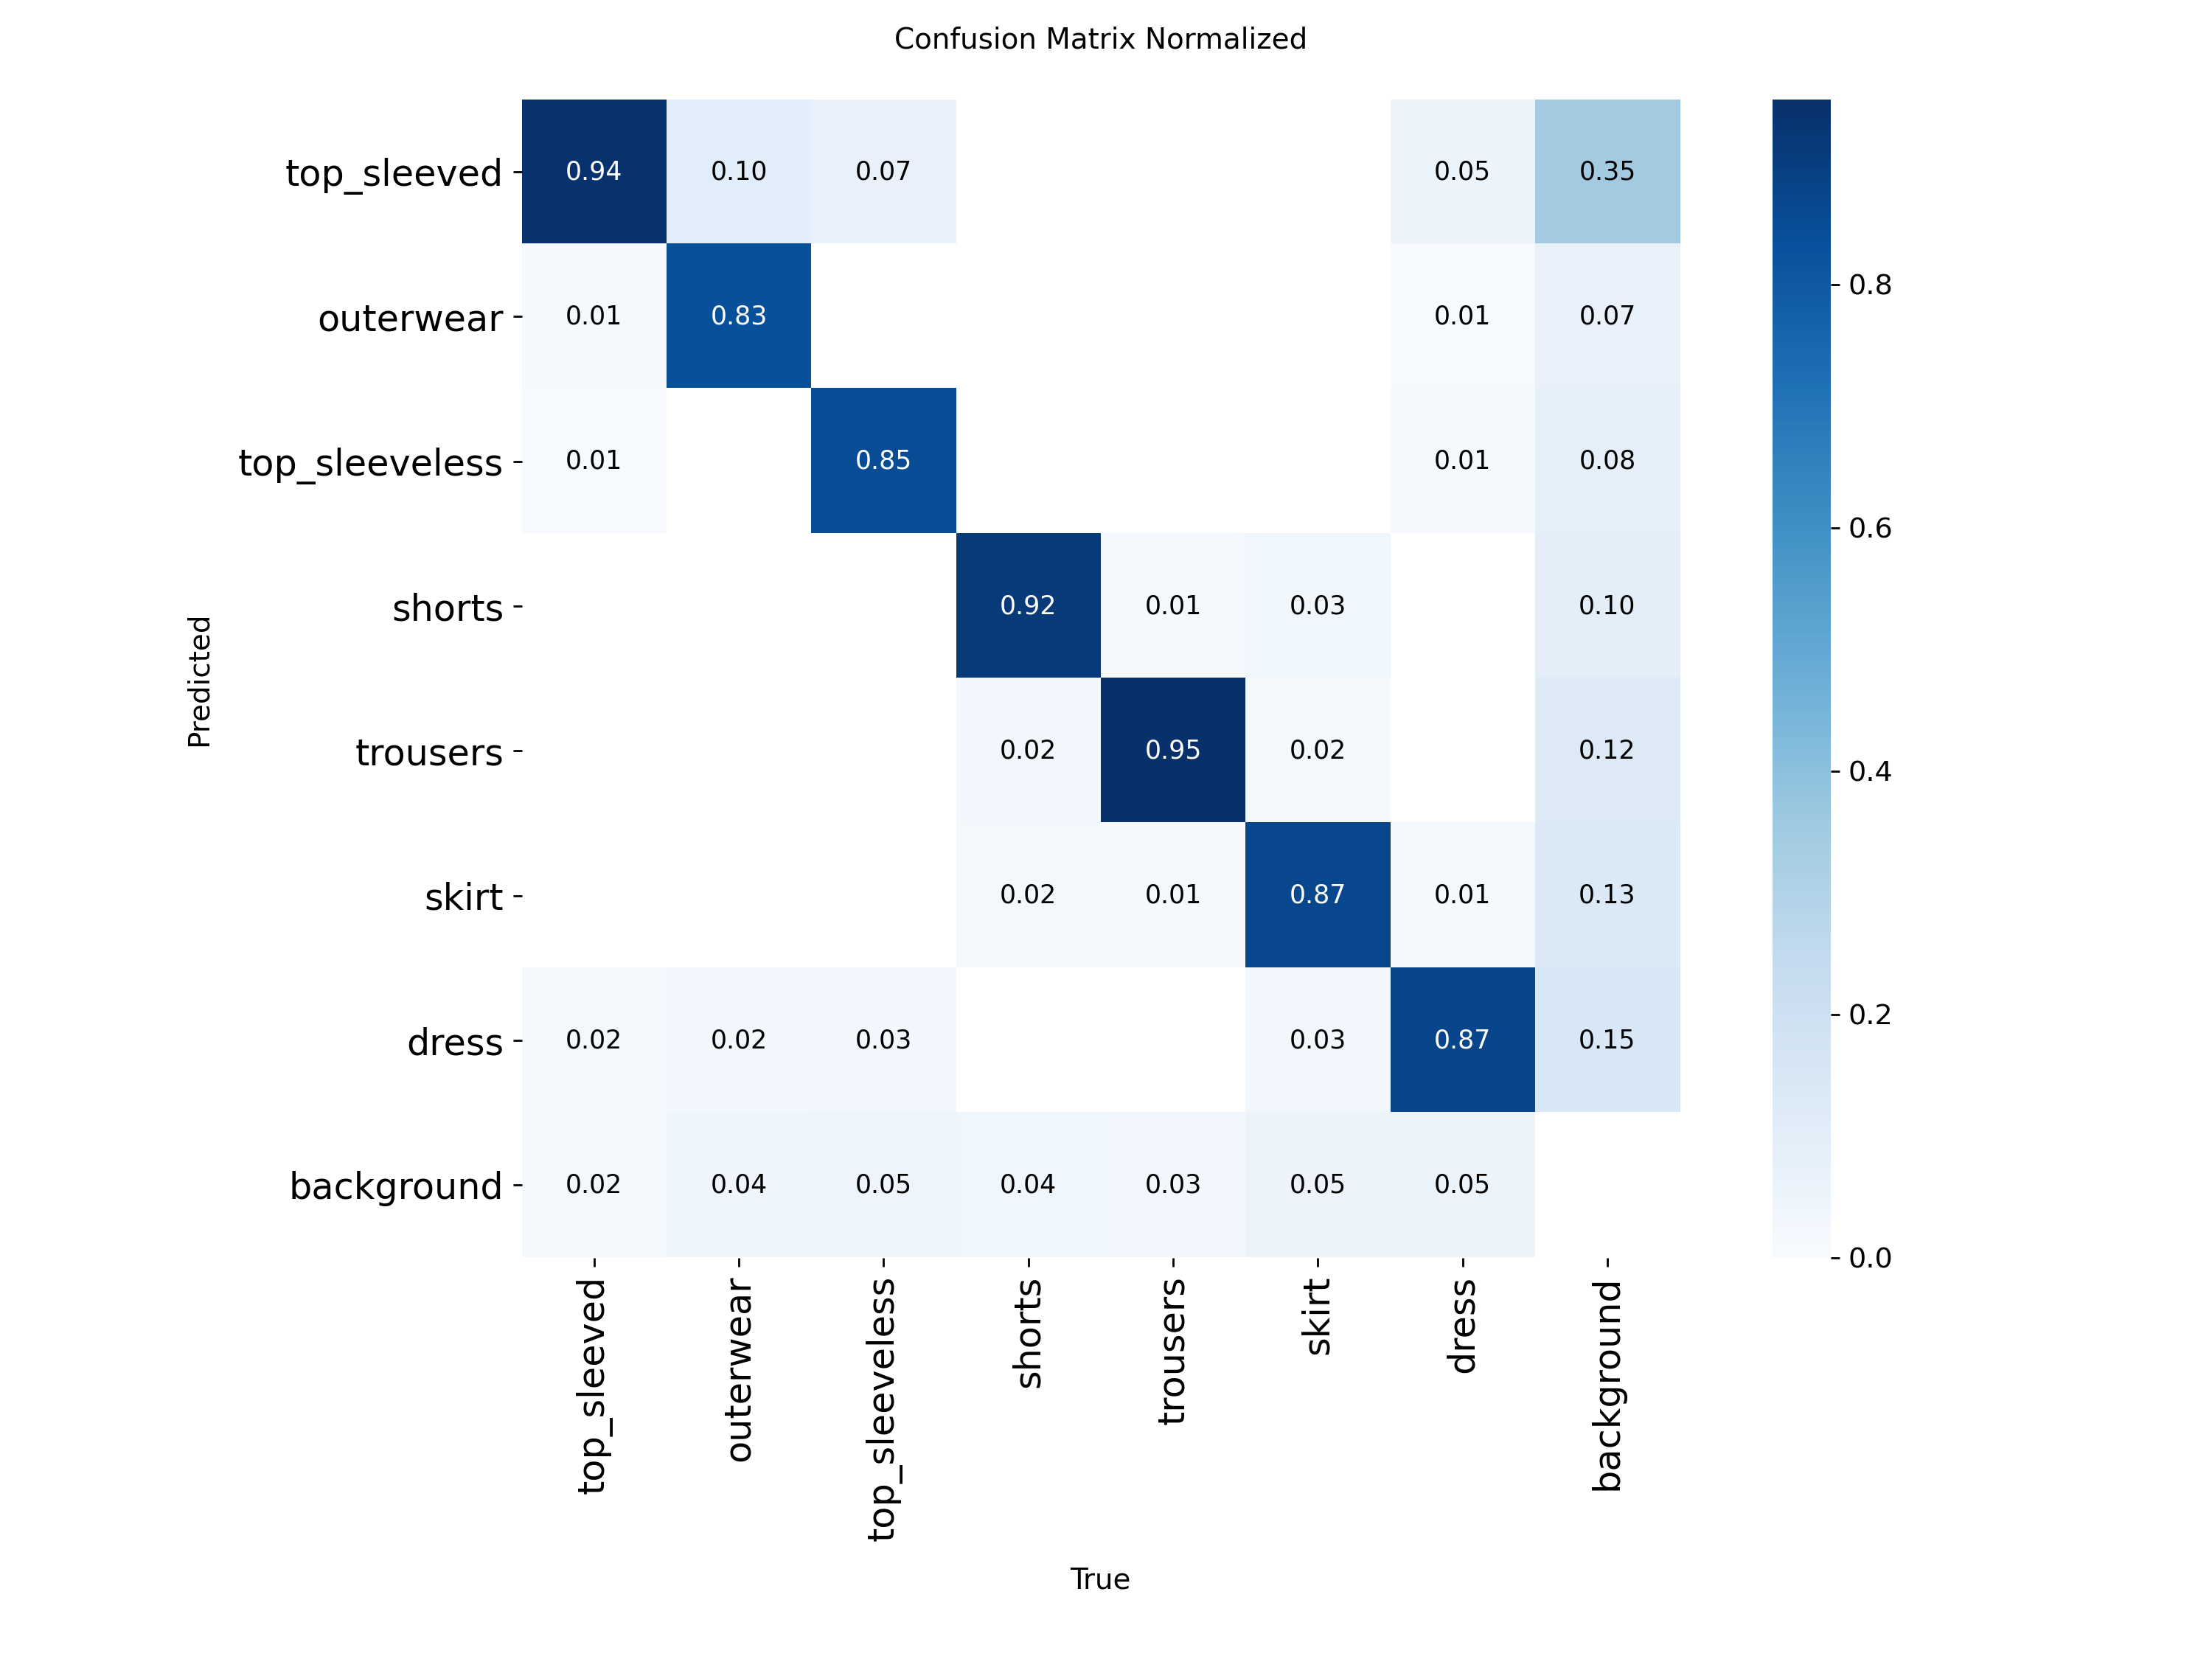
\includegraphics[width=0.90\linewidth]{appendix/experiments/confusion_mat_yolo26n_df2.png}
  \caption{Нормализованная матрица ошибок для YOLO26n на DeepFashion2-7c.}
  \label{fig:appendix_confusion_yolo26n_df2}
\end{figure}

На рисунке~\ref{fig:appendix_confusion_yolo26n_df2} видно, что YOLO26n на DeepFashion2 уверенно
отделяет основные классы одежды, но ошибки в сторону background сохраняют риск пропуска части
textured ROI.

\begin{figure}[!htbp]
  \centering
  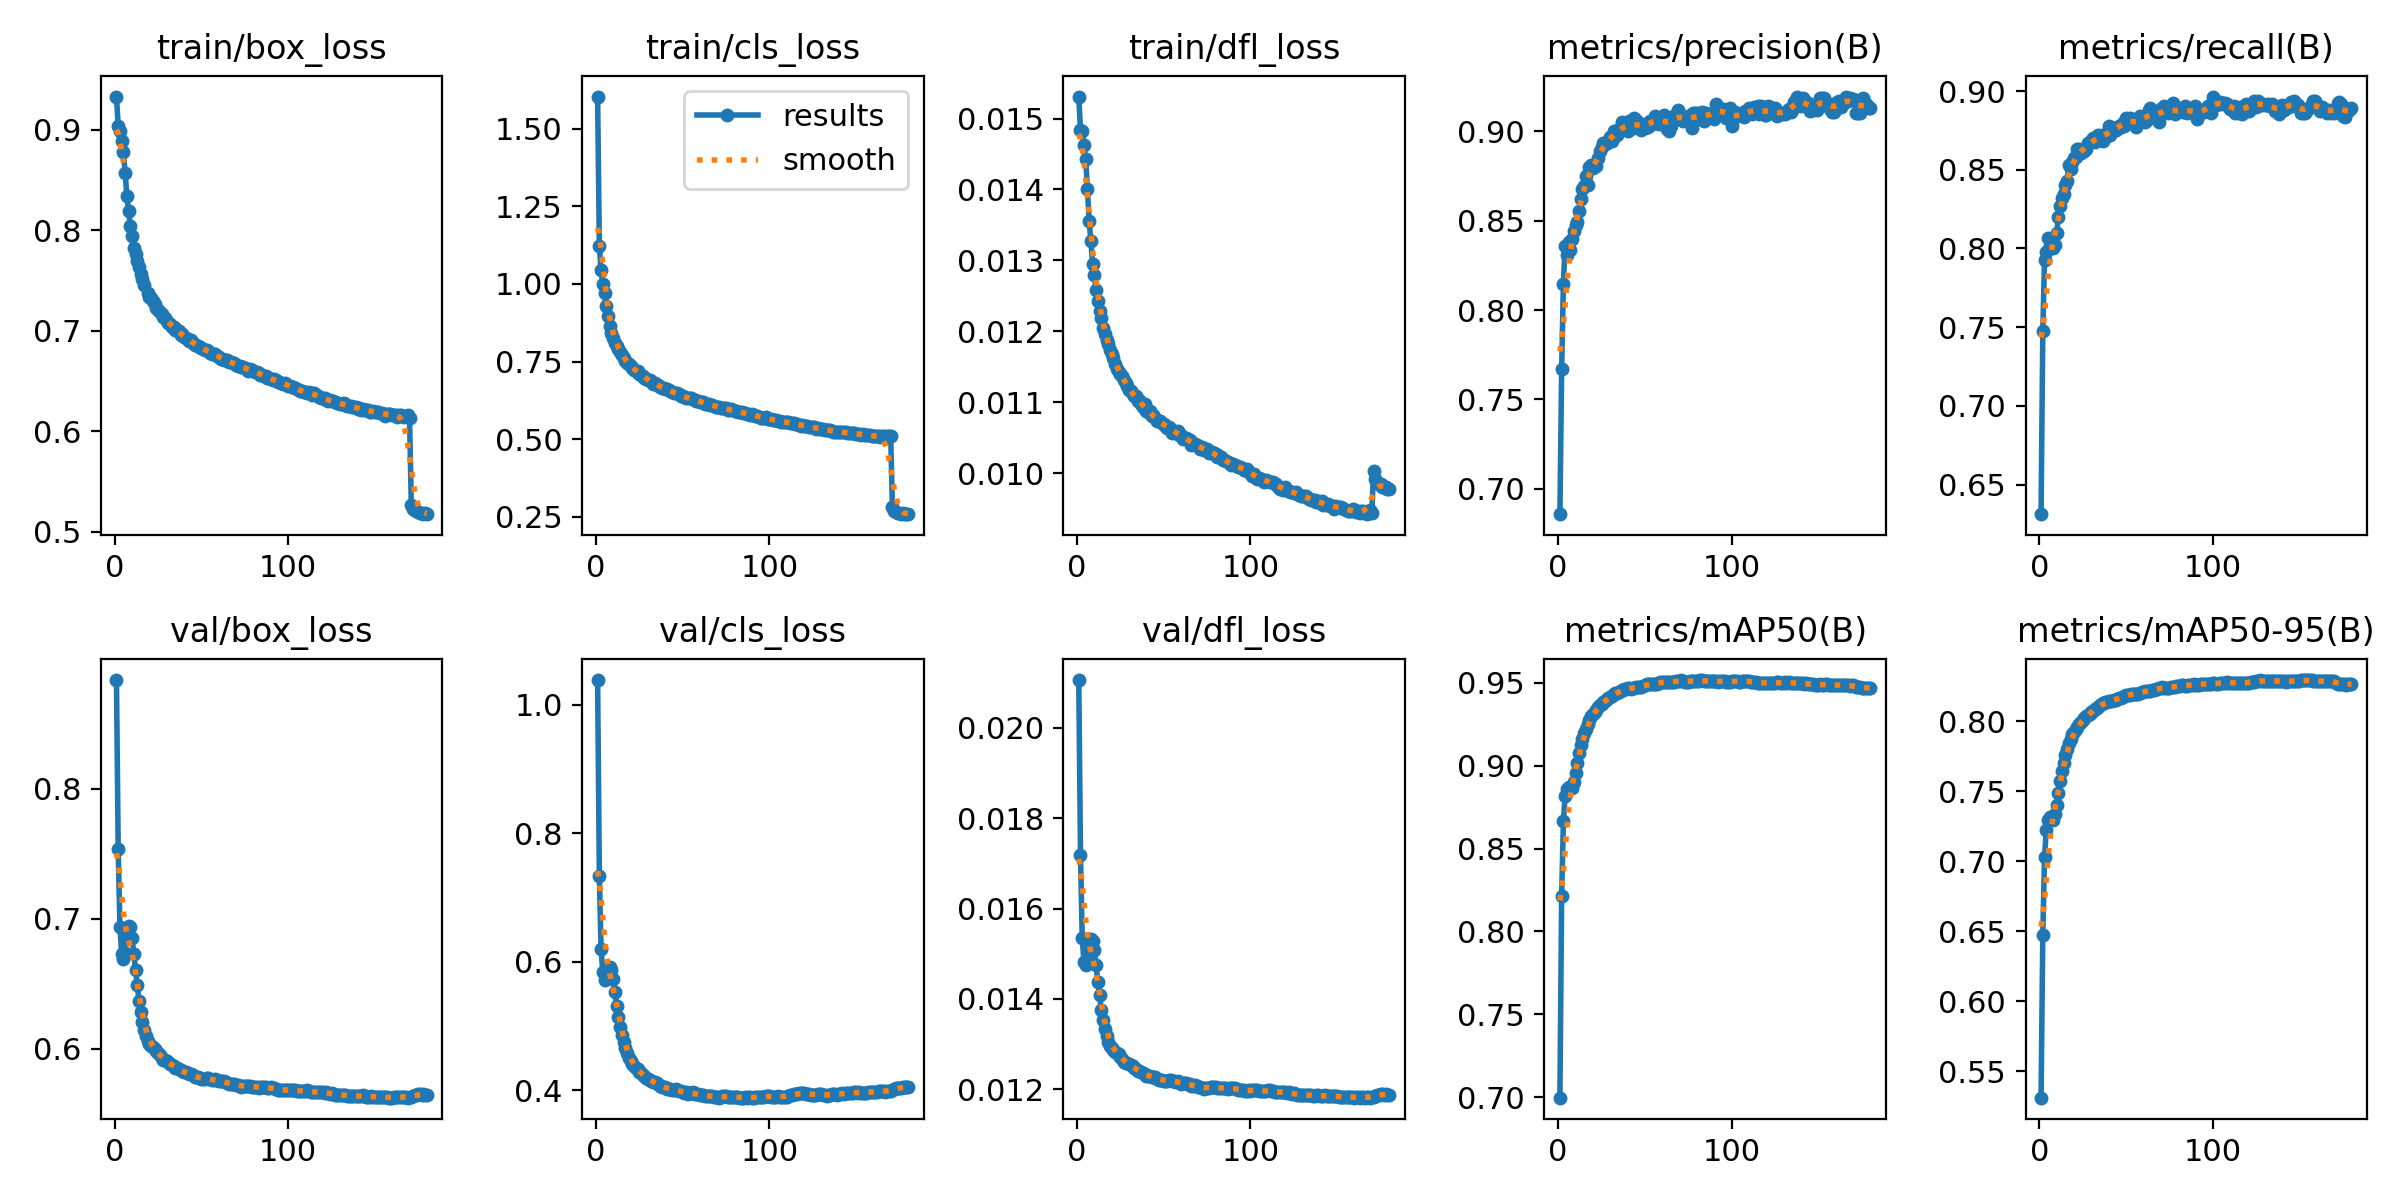
\includegraphics[width=0.96\linewidth]{appendix/experiments/results_yolo26n_df2.png}
  \caption{Динамика метрик обучения YOLO26n на DeepFashion2-7c.}
  \label{fig:appendix_results_yolo26n_df2}
\end{figure}

По рисунку~\ref{fig:appendix_results_yolo26n_df2} видно, что кривые обучения стабилизируются
без резких провалов. Поэтому итоговые метрики YOLO26n-DF2 можно интерпретировать как результат
сходимости, а не случайный выброс последней эпохи.

% -------------------- YOLO26n, DeepFashion2+Fashionpedia --------------------

\begin{figure}[!htbp]
  \centering
  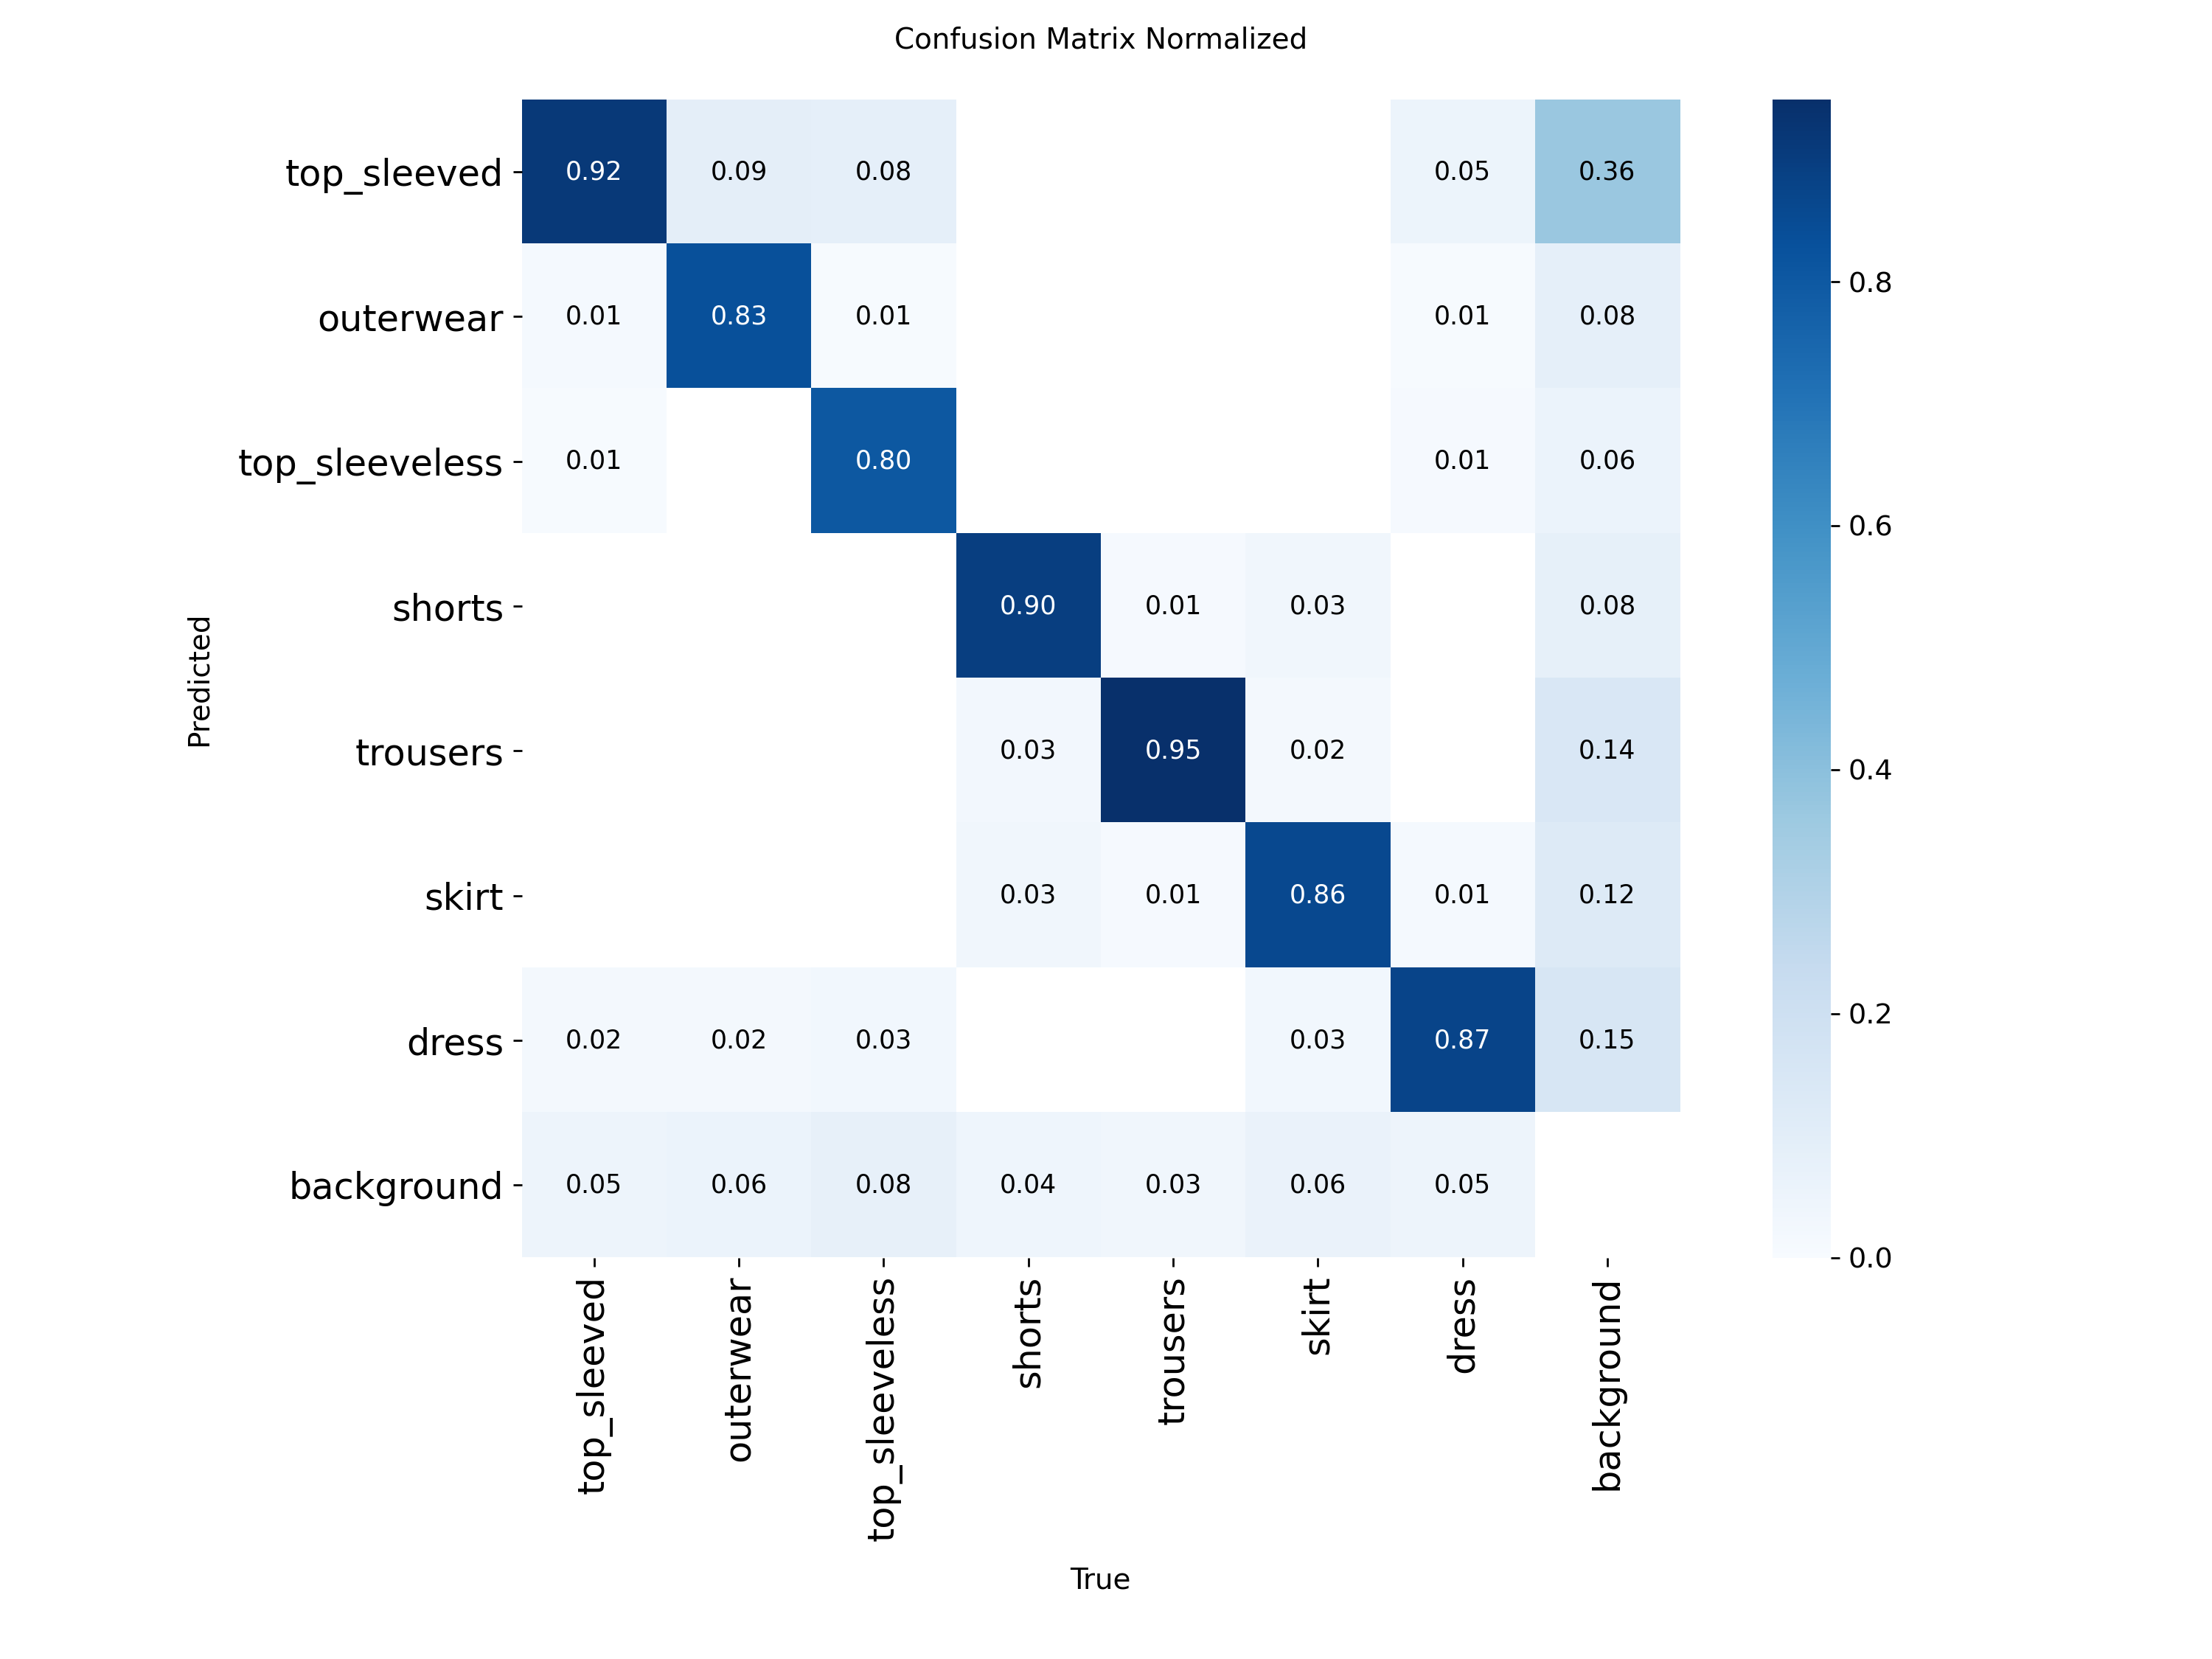
\includegraphics[width=0.90\linewidth]{appendix/experiments/confusion_mat_yolo26n_df2_fp.png}
  \caption{Нормализованная матрица ошибок для YOLO26n на объединенном наборе
      DeepFashion2+Fashionpedia.}
  \label{fig:appendix_confusion_yolo26n_df2_fp}
\end{figure}

Рисунок~\ref{fig:appendix_confusion_yolo26n_df2_fp} показывает, что на объединенном наборе
диагональ остается высокой, но \texttt{top\_sleeveless} и \texttt{outerwear} остаются самыми
чувствительными классами.

\begin{figure}[!htbp]
  \centering
  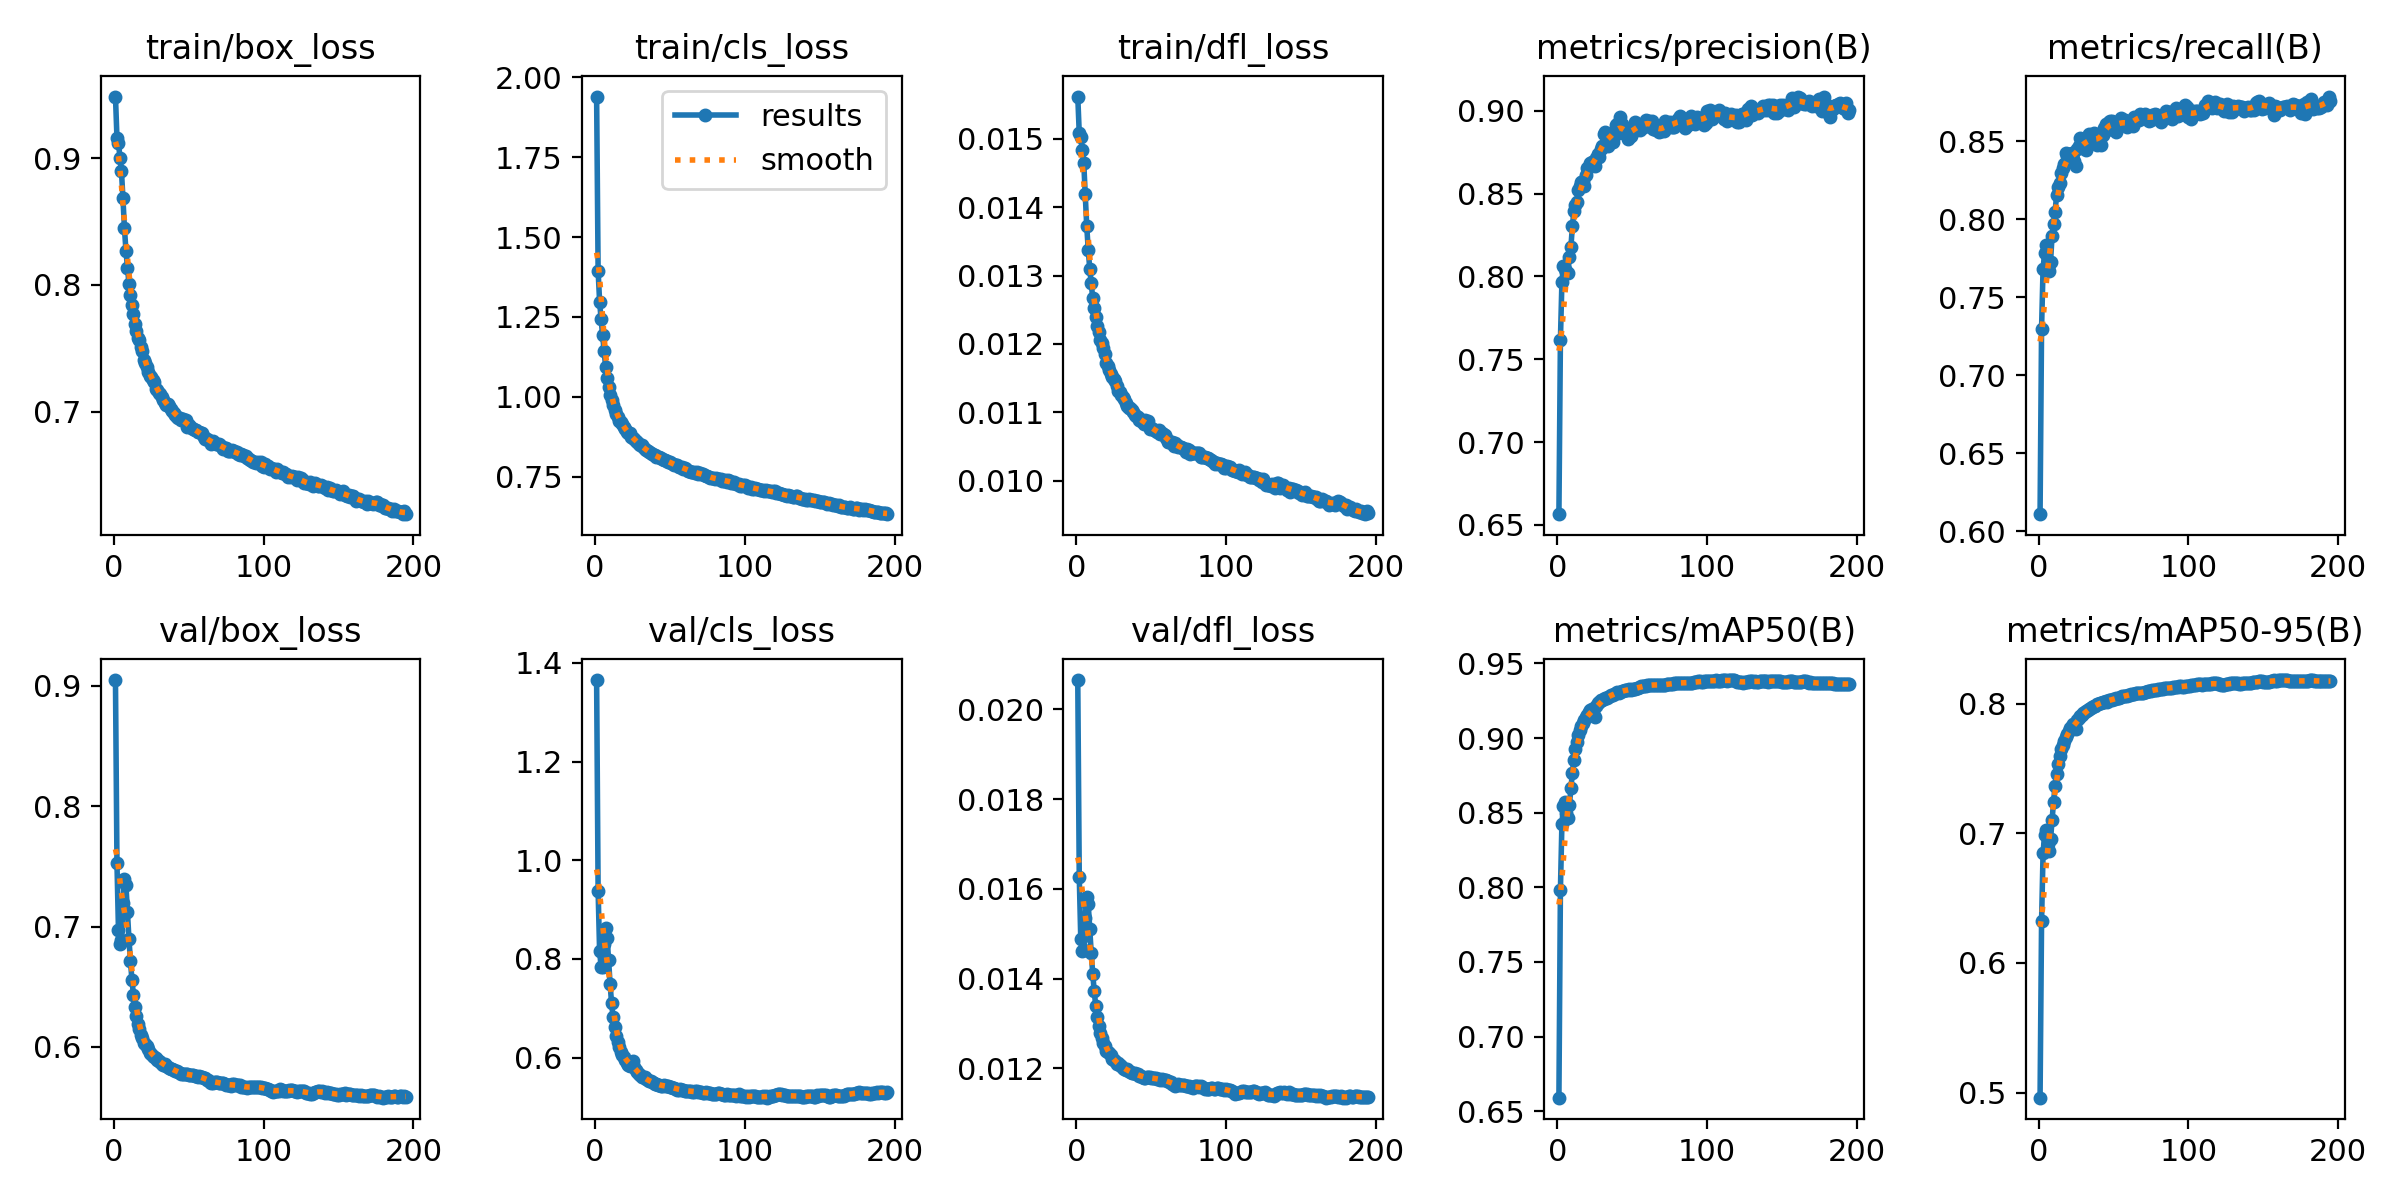
\includegraphics[width=0.96\linewidth]{appendix/experiments/results_yolo26n_df2_fp.png}
  \caption{Динамика метрик обучения YOLO26n на объединенном наборе DeepFashion2+Fashionpedia.}
  \label{fig:appendix_results_yolo26n_df2_fp}
\end{figure}

Рисунок~\ref{fig:appendix_results_yolo26n_df2_fp} показывает, что объединенный датасет не
ломает обучение YOLO26n: метрики выходят на плато, а loss-кривые снижаются. Это подтверждает
пригодность объединенной таксономии.

% -------------------- YOLO26s, DeepFashion2 --------------------

\begin{figure}[!htbp]
  \centering
  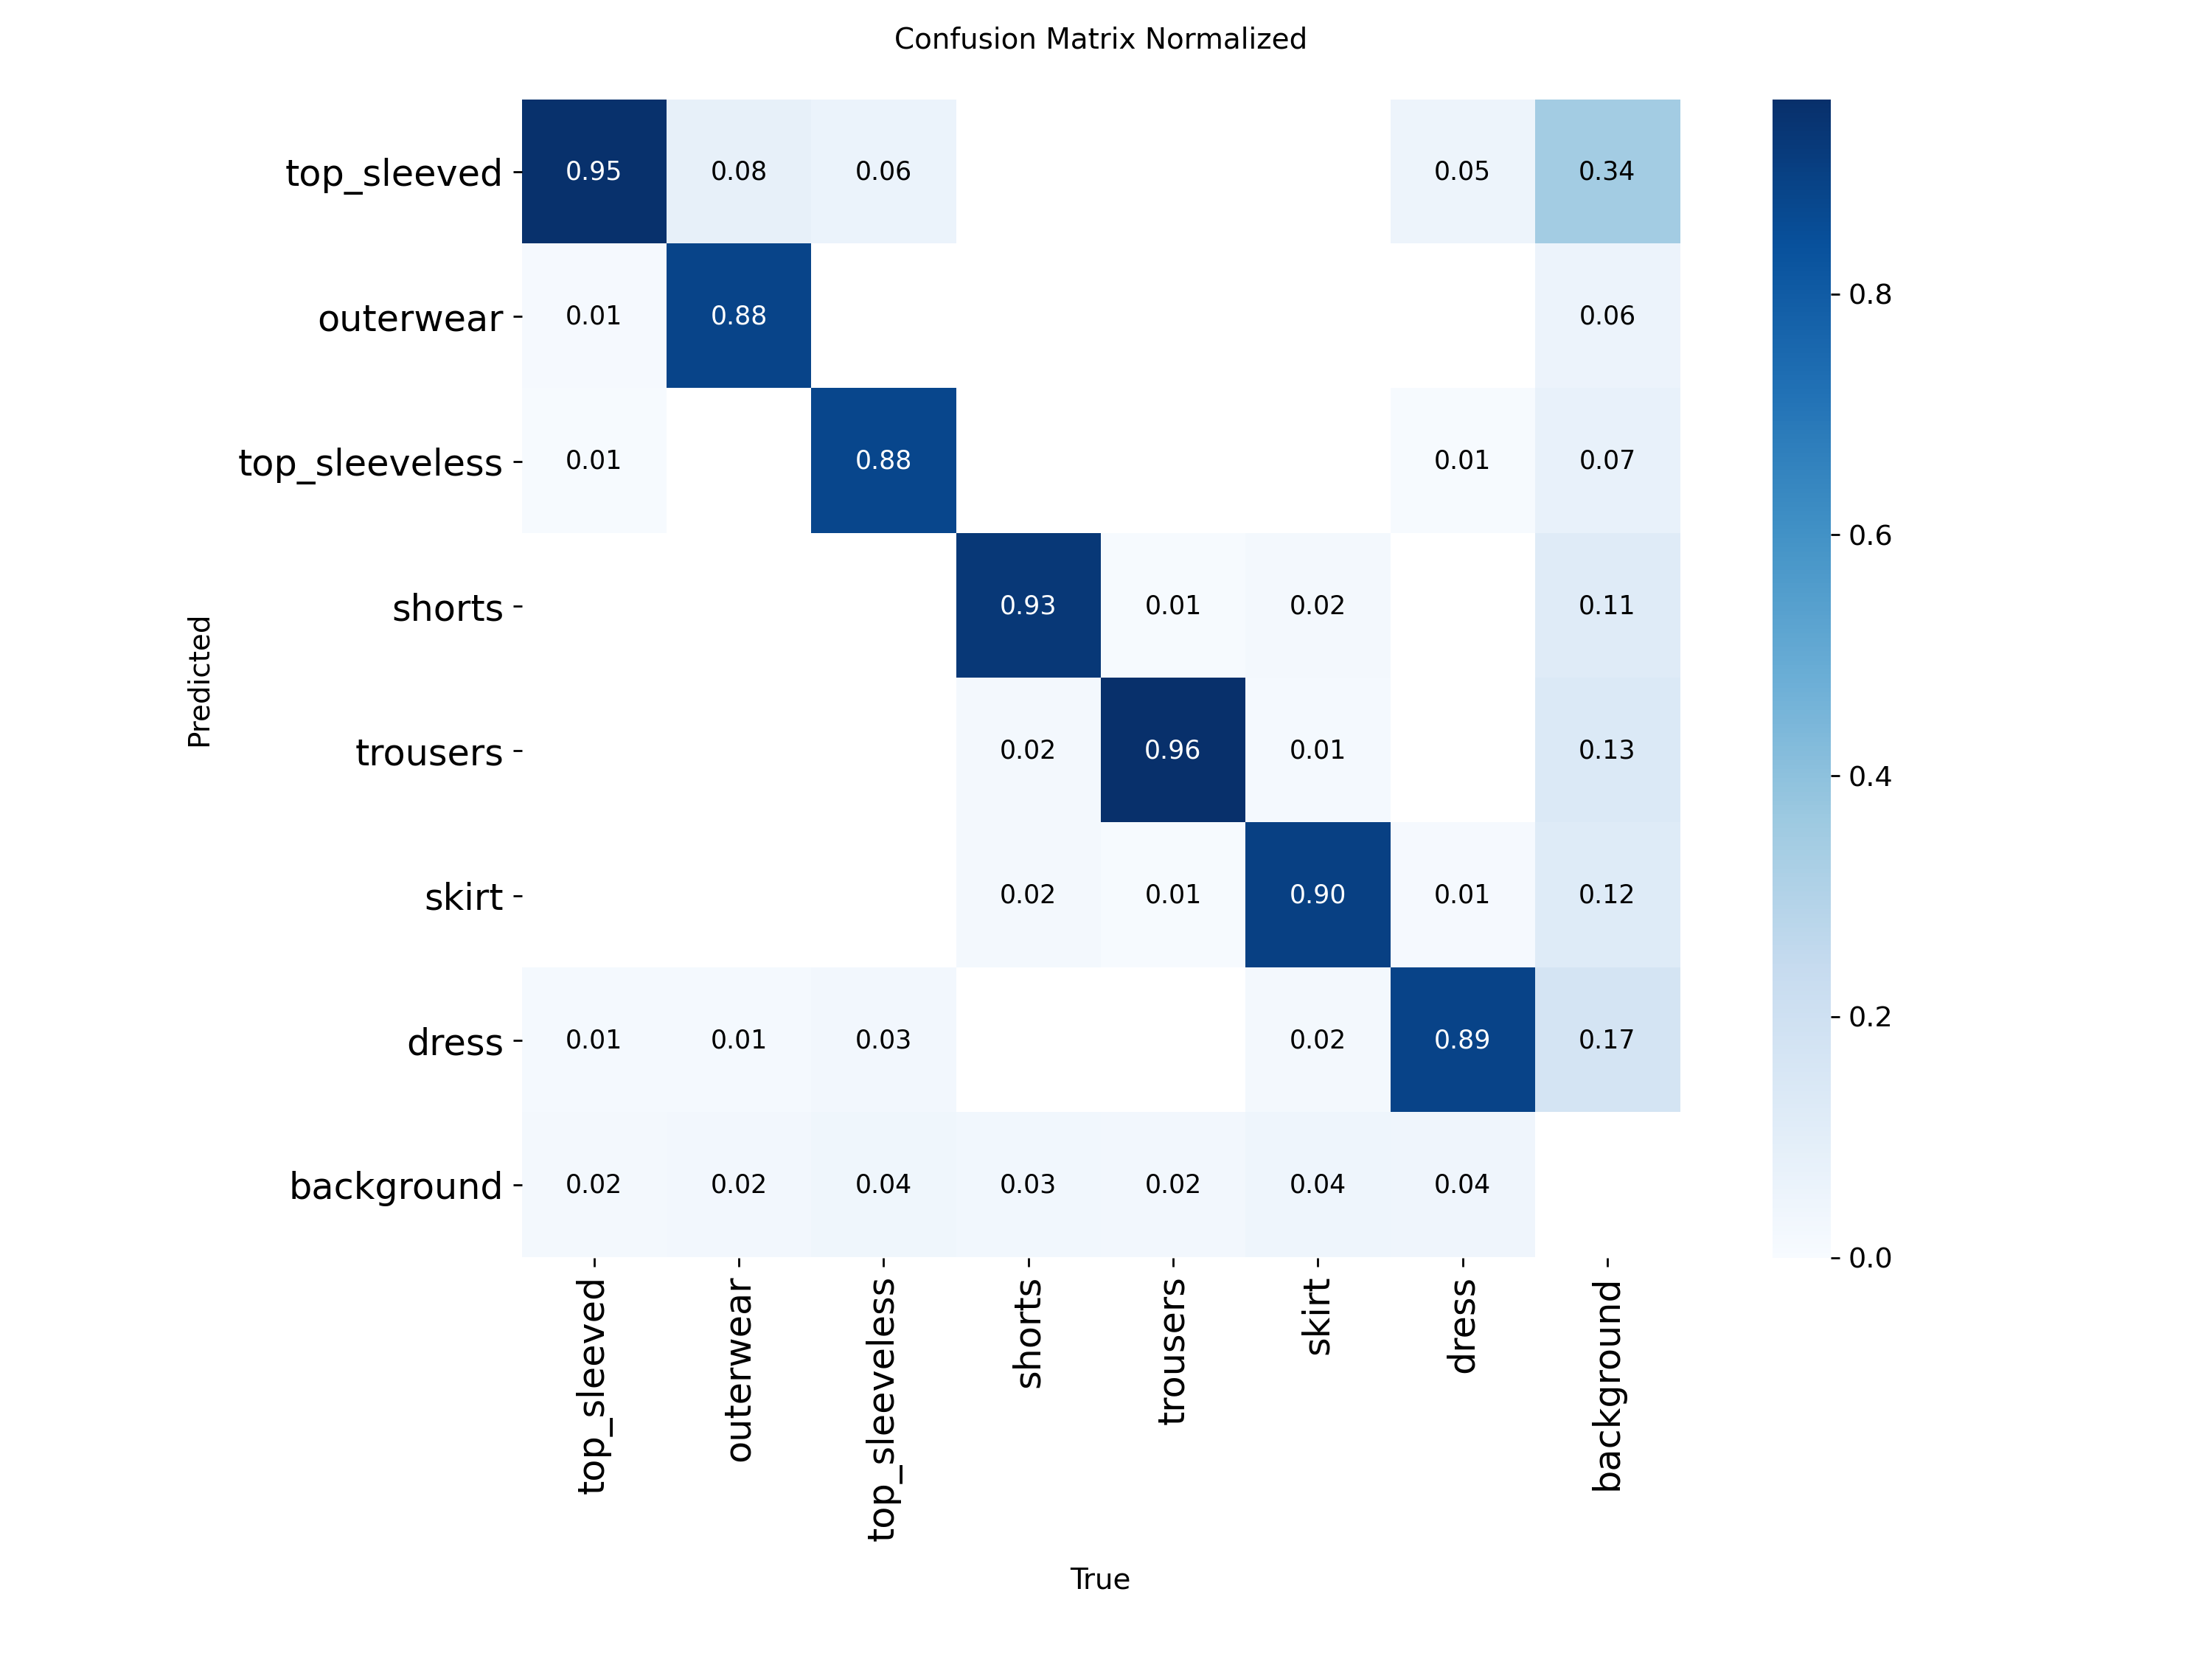
\includegraphics[width=0.90\linewidth]{appendix/experiments/confusion_mat_yolo26s_df2.png}
  \caption{Нормализованная матрица ошибок для YOLO26s на DeepFashion2-7c.}
  \label{fig:appendix_confusion_yolo26s_df2}
\end{figure}

На рисунке~\ref{fig:appendix_confusion_yolo26s_df2} видно, что YOLO26s улучшает диагональ для
ряда классов, но не устраняет полностью ошибки близких категорий одежды и переходы в background.

\begin{figure}[!htbp]
  \centering
  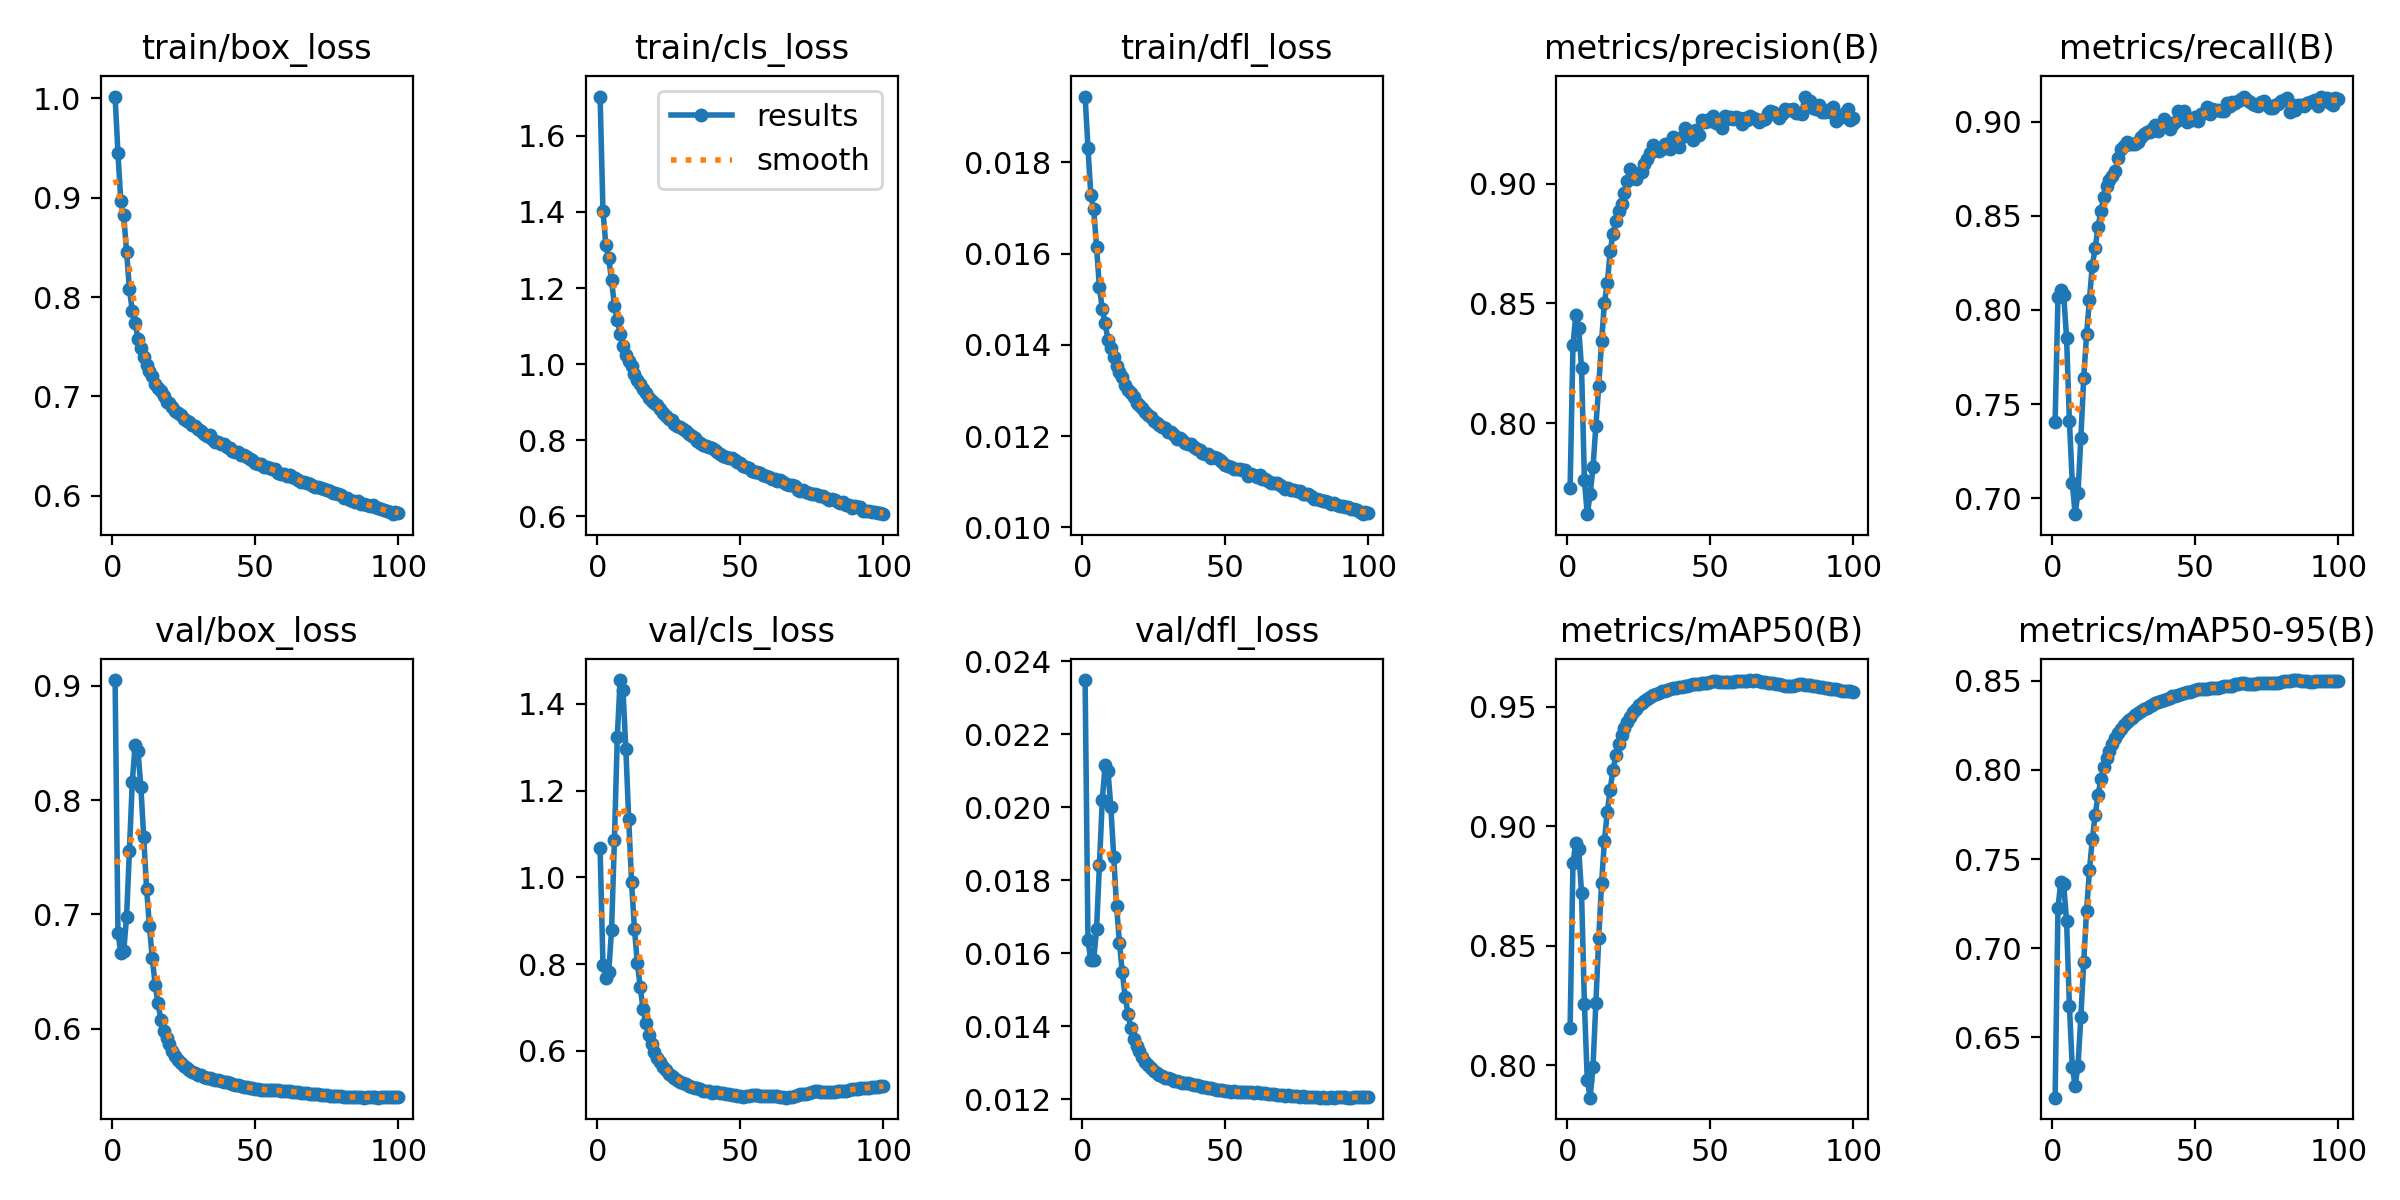
\includegraphics[width=0.96\linewidth]{appendix/experiments/results_yolo26s_df2.png}
  \caption{Динамика метрик обучения YOLO26s на DeepFashion2-7c.}
  \label{fig:appendix_results_yolo26s_df2}
\end{figure}

Рисунок~\ref{fig:appendix_results_yolo26s_df2} показывает устойчивую сходимость YOLO26s, но ее
преимущество нужно сопоставлять с четырехкратной стоимостью относительно YOLO26n.

% -------------------- YOLO26s, DeepFashion2+Fashionpedia --------------------

\begin{figure}[!htbp]
  \centering
  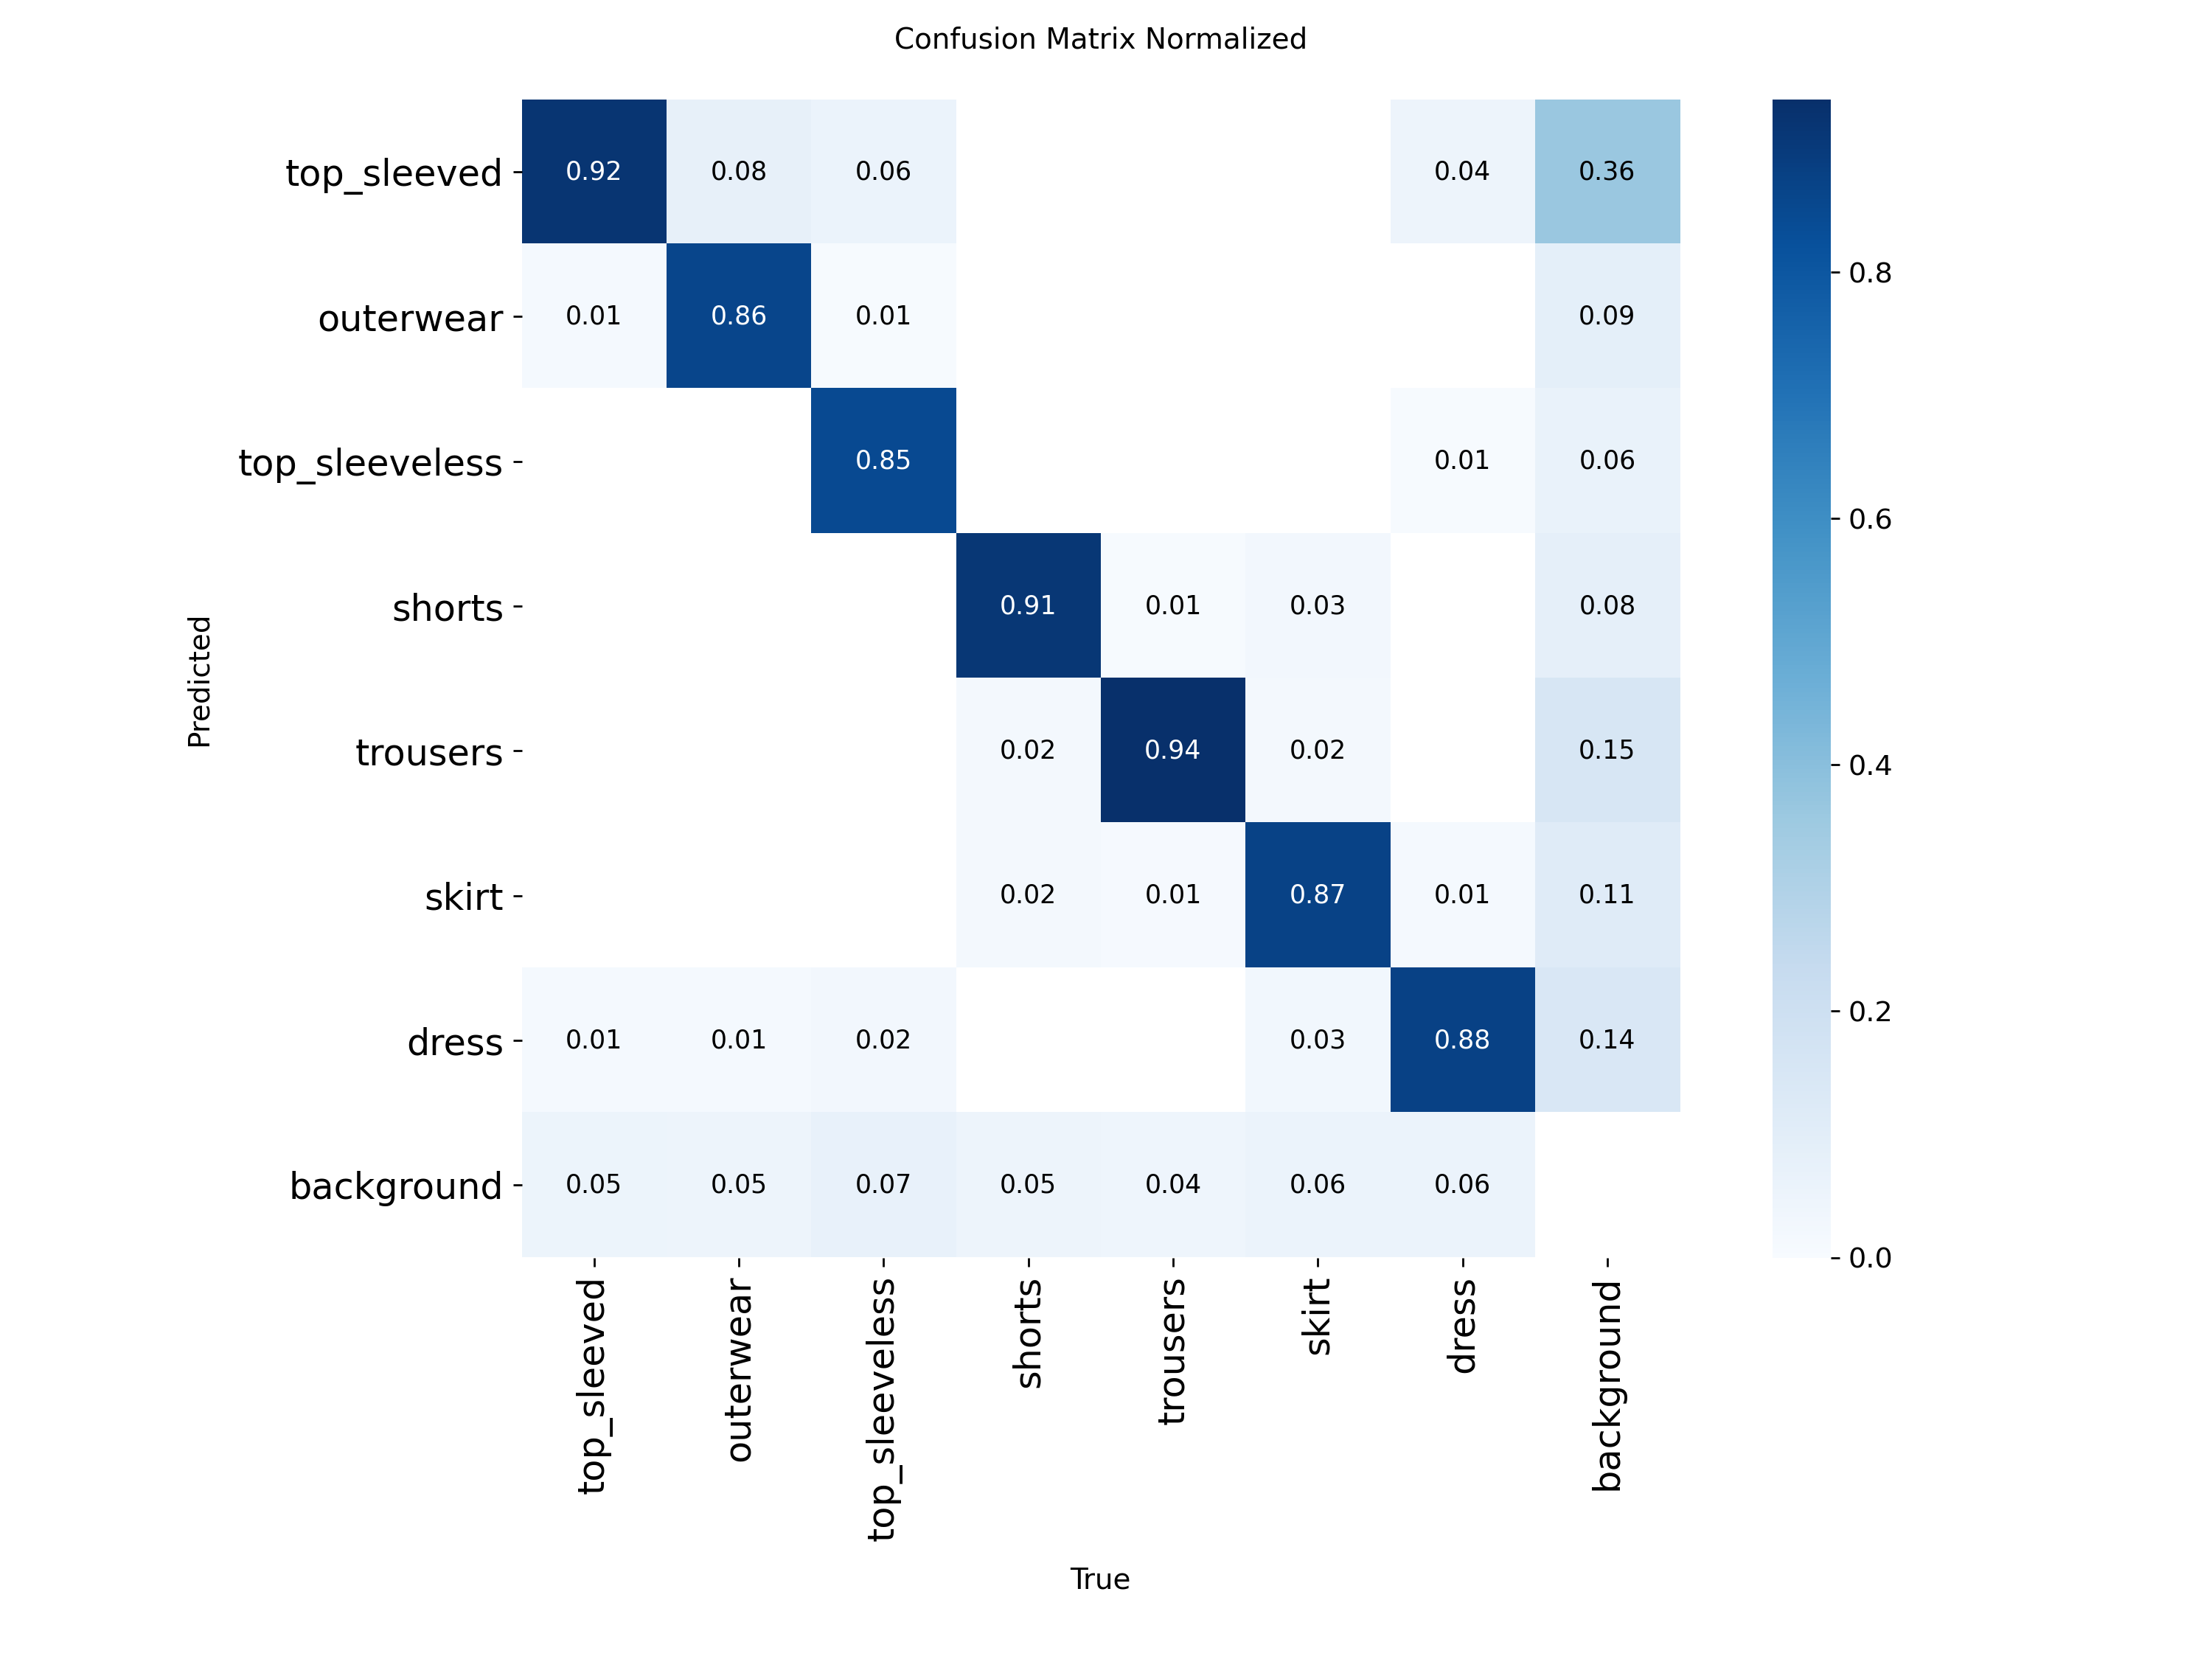
\includegraphics[width=0.90\linewidth]{appendix/experiments/confusion_mat_yolo26s_df2_fp.png}
  \caption{Нормализованная матрица ошибок для YOLO26s на объединенном наборе
      DeepFashion2+Fashionpedia.}
  \label{fig:appendix_confusion_yolo26s_df2_fp}
\end{figure}

На рисунке~\ref{fig:appendix_confusion_yolo26s_df2_fp} видно, что на объединенном наборе YOLO26s
сохраняет сильную диагональ, но практическое преимущество над YOLO26n остается умеренным для
CPU-first задачи.

\begin{figure}[!htbp]
  \centering
  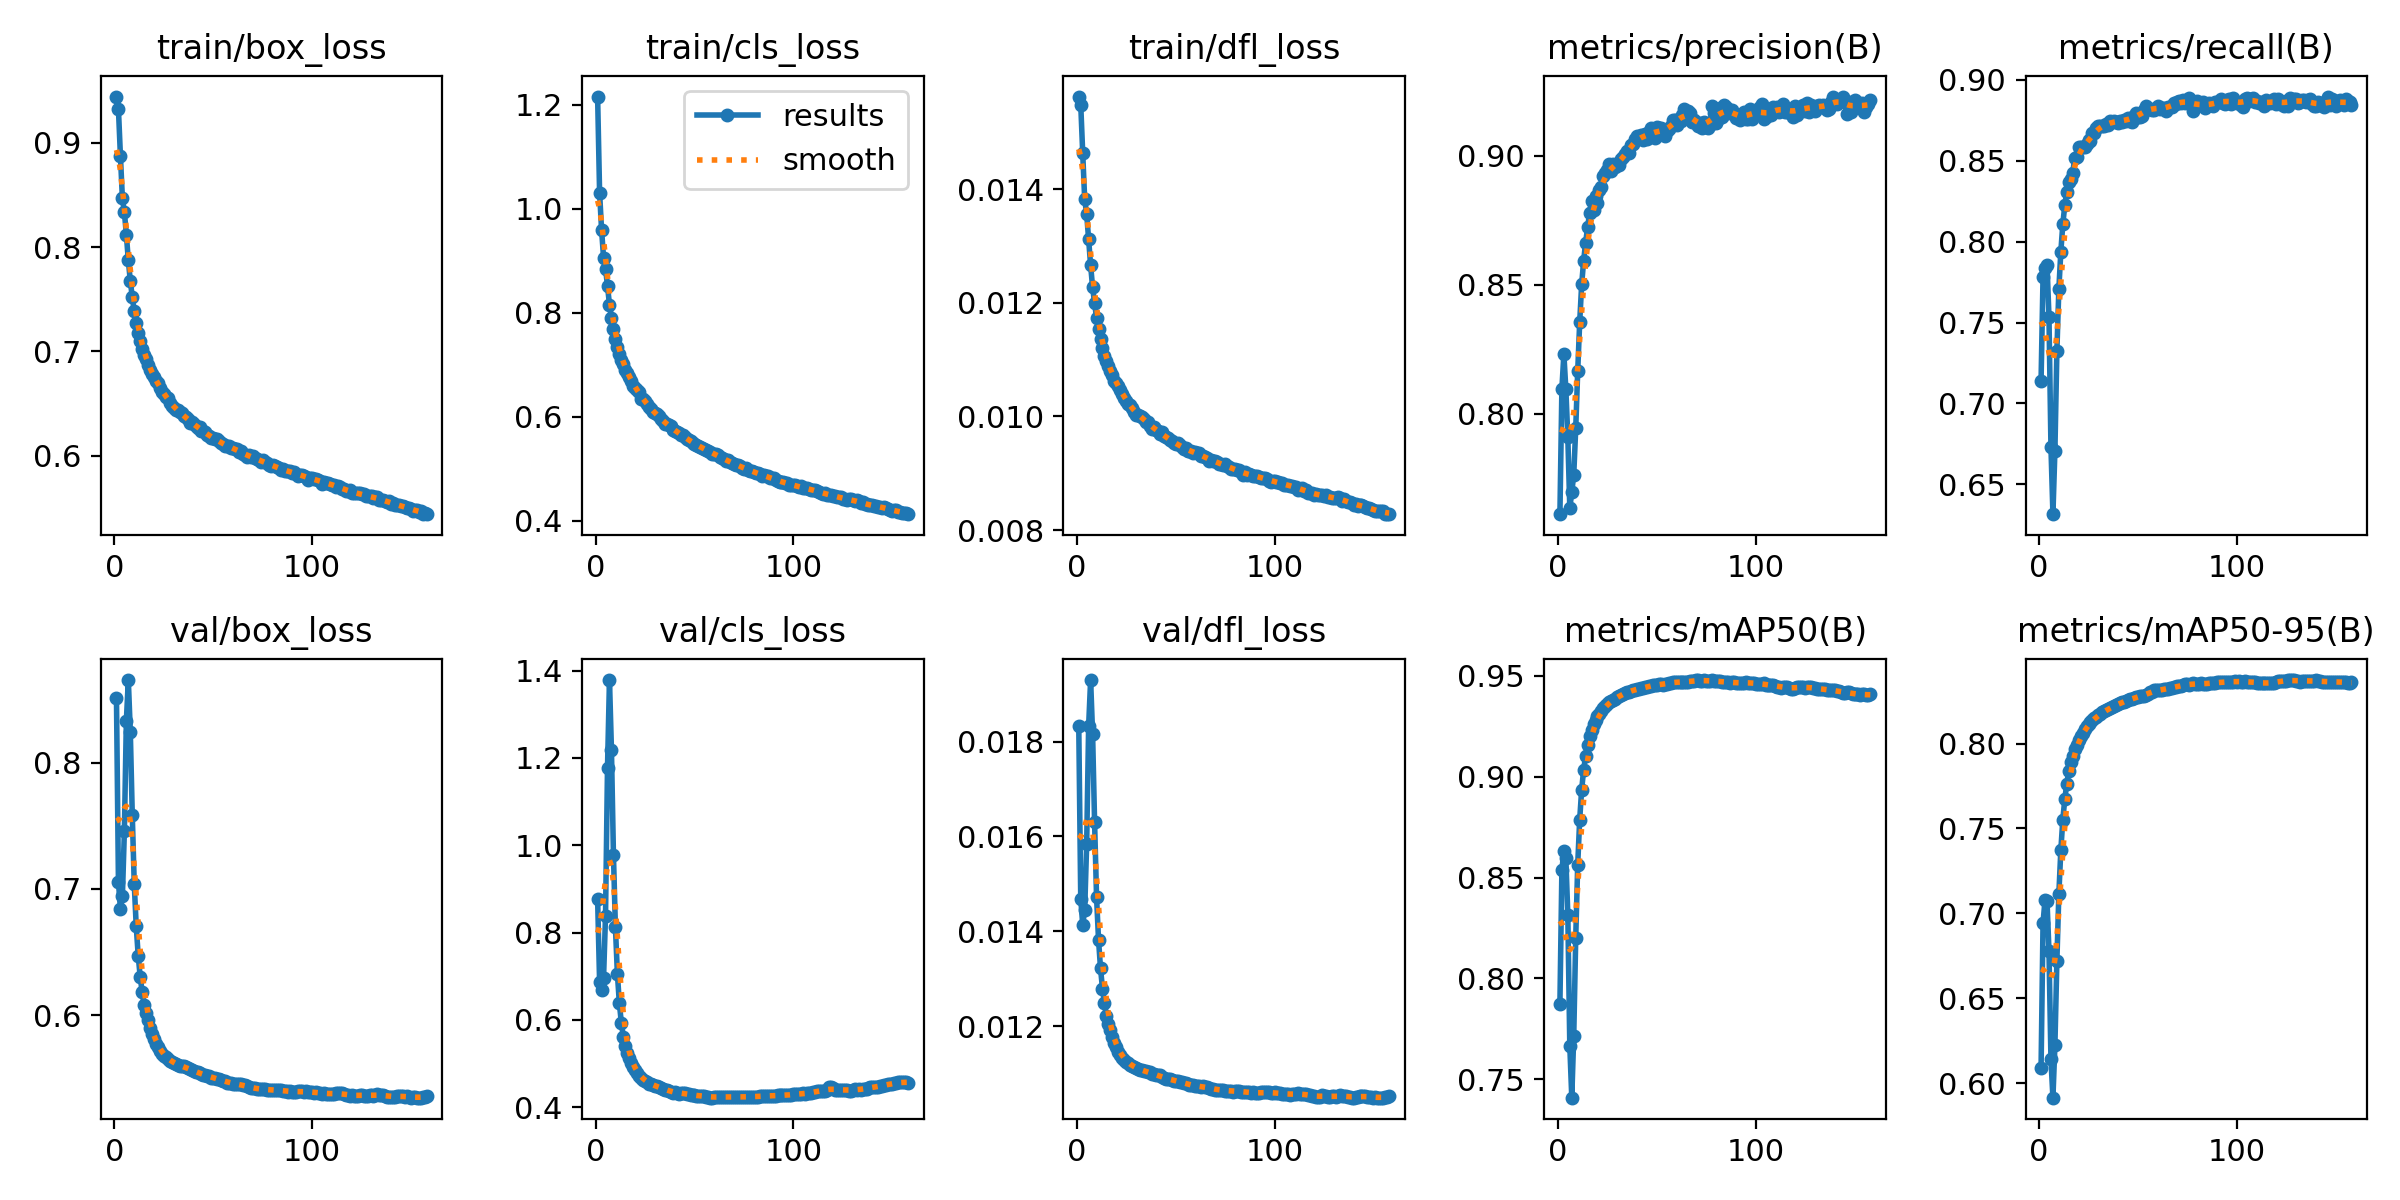
\includegraphics[width=0.96\linewidth]{appendix/experiments/results_yolo26s_df2_fp.png}
  \caption{Динамика метрик обучения YOLO26s на объединенном наборе DeepFashion2+Fashionpedia.}
  \label{fig:appendix_results_yolo26s_df2_fp}
\end{figure}

Рисунок~\ref{fig:appendix_results_yolo26s_df2_fp} подтверждает работоспособность обучения
YOLO26s на объединенном наборе, но не отменяет deployment-ограничение по размеру и GFLOPs.

Сравнение всех диагностических рисунков показывает, что интерпретация качества модели должна
учитывать как итоговую структуру ошибок, так и динамику обучения. Для задачи textured ROI
особенно важны не только ошибки между близкими классами одежды, но и случаи перехода объекта в
background. Если модель путает близкие типы одежды, но сохраняет корректное покрытие области,
downstream-кодировщик все равно может использовать такую область как textured ROI. Гораздо
опаснее ситуации, когда значимая область не выделяется вовсе или когда ROI становится чрезмерно
широкой и начинает расходовать битовый бюджет на второстепенные фрагменты кадра.

% A.6 Визуализация labels для датасетных конфигураций

\section{Визуализация labels для датасетных конфигураций}

\begin{figure}[!htbp]
  \centering
  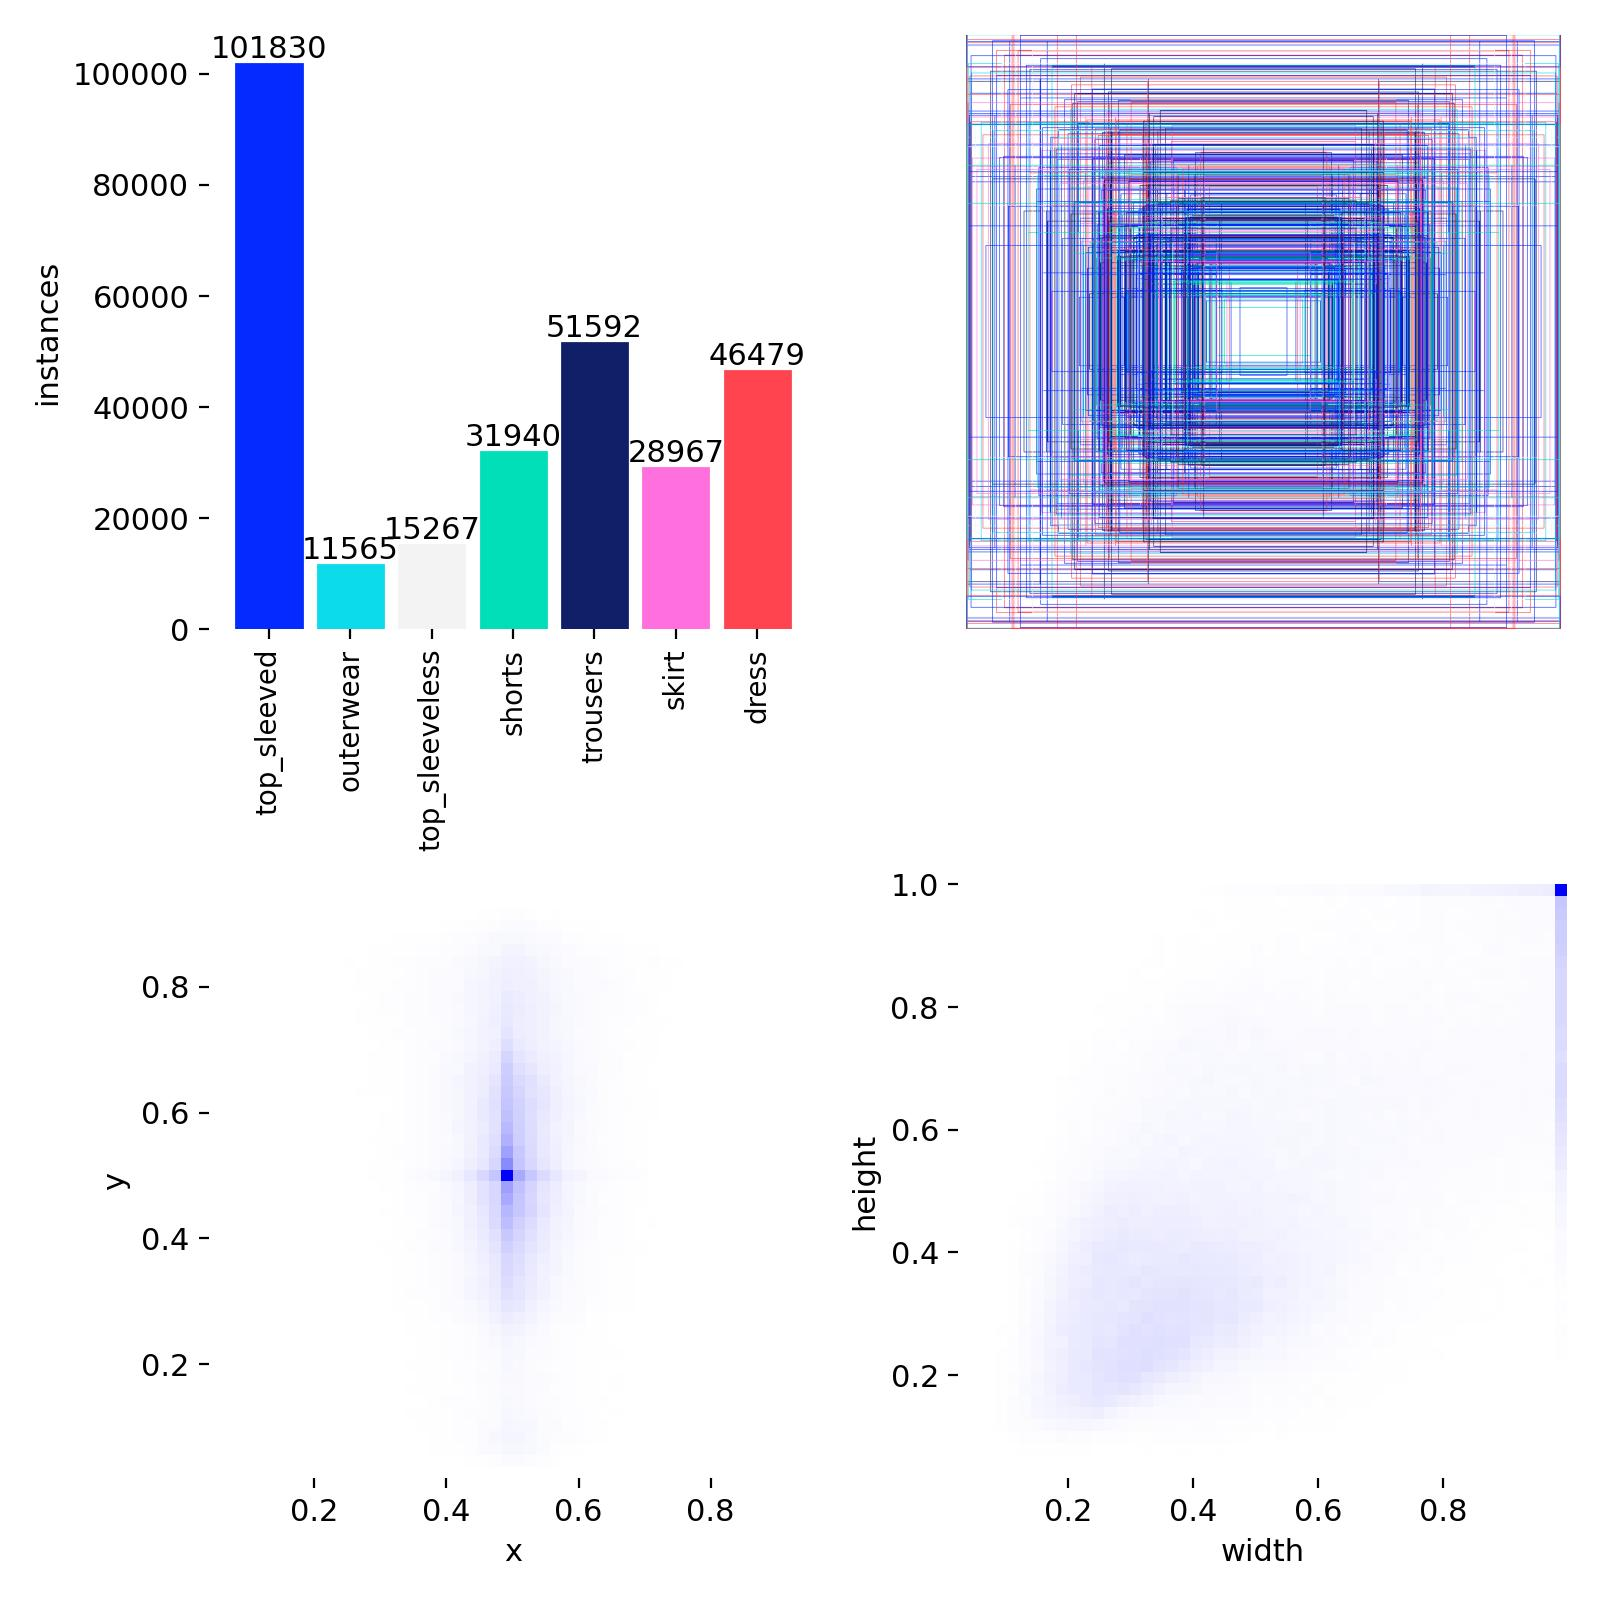
\includegraphics[width=0.96\linewidth]{appendix/labels/labels_df2.jpg}
  \caption{Визуализация labels для DeepFashion2-7c.}
  \label{fig:appendix_labels_deepfashion2}
\end{figure}

Рисунок~\ref{fig:appendix_labels_deepfashion2} показывает структуру разметки DeepFashion2-7c:
распределение классов, центры bbox, ширину и высоту bbox, а также совместное распределение
геометрии объектов. Для этого набора характерны концентрация объектов около центра кадра,
преобладание крупных bbox и перекос в пользу верхней одежды. В textured ROI это полезно для
локализации одежды, но требует контроля area budget: крупные области могут конкурировать с
text/face ROI.

\begin{figure}[!htbp]
  \centering
  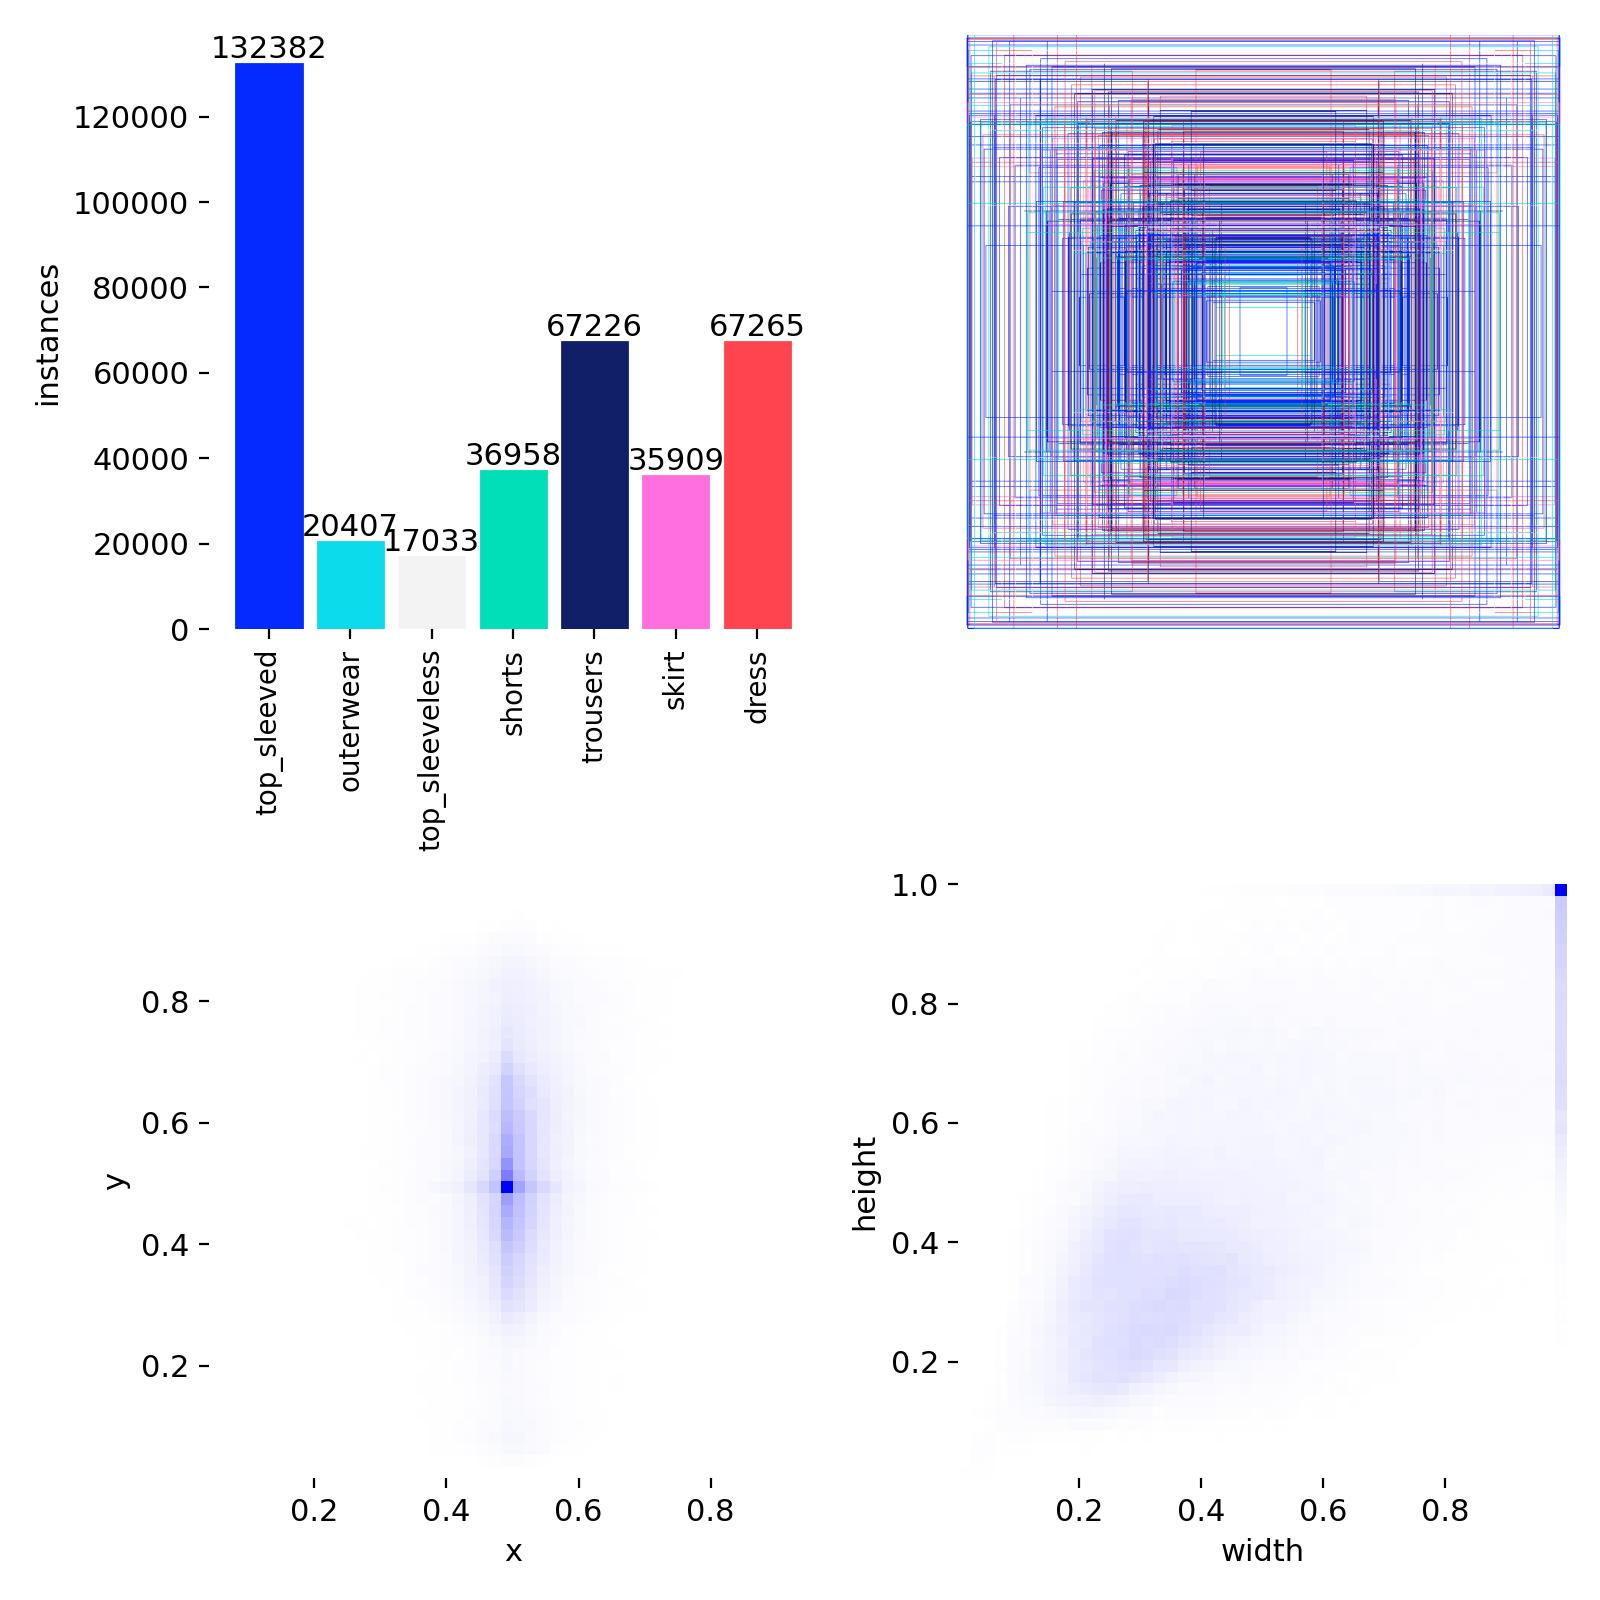
\includegraphics[width=0.96\linewidth]{appendix/labels/labels_df2_fp.jpg}
  \caption{Визуализация labels для объединенного набора DeepFashion2+Fashionpedia-7c.}
  \label{fig:appendix_labels_merged}
\end{figure}

Рисунок~\ref{fig:appendix_labels_merged} показывает структуру labels после объединения
DeepFashion2 и Fashionpedia в единую 7-классовую таксономию. Объединенный набор содержит больше
изображений и объектов, расширяет геометрию примеров, но не устраняет дисбаланс классов:
наиболее частые категории формируют большую часть обучающего сигнала, тогда как редкие классы
требуют отдельного контроля через
per-class AP и confusion matrix.

\clearpage
\renewcommand{\thesection}{B.\arabic{section}}
\setcounter{section}{0}
\setcounter{table}{0}
\setcounter{figure}{0}
\setcounter{lstlisting}{0}
\renewcommand{\thetable}{B.\arabic{table}}
\renewcommand{\thefigure}{B.\arabic{figure}}
\renewcommand{\thelstlisting}{B.\arabic{lstlisting}}
\renewcommand{\theHsection}{appB.\arabic{section}}
\renewcommand{\theHtable}{appB.\arabic{table}}
\renewcommand{\theHfigure}{appB.\arabic{figure}}
\renewcommand{\theHlstlisting}{appB.\arabic{lstlisting}}

% B.1 Команда чистого измерения задержки

\section{Команда чистого измерения задержки}

Листинг~\ref{lst:appendix_latency_benchmark} показывает параметризованный запуск
\texttt{idet\_app} для чистого измерения задержки. В этом режиме отключены отрисовка, выгрузка
геометрии и подробный вывод, поэтому результат отражает задержку пути среды выполнения, а не
стоимость диагностической записи.

\begin{lstlisting}[
    caption={Параметризованный запуск \texttt{idet\_app} для чистого измерения задержки},
    label={lst:appendix_latency_benchmark}
  ]
idet_app \
  --mode cloth \
  --model <onnx-model> \
  --image <input-image> \
  --bind_io 1 \
  --runtime_policy 1 \
  --soft_mem_bind 1 \
  --cpu_placement latency \
  --bench_iters 30 \
  --warmup_iters 5 \
  --is_draw 0 \
  --is_dump 0 \
  --verbose 0 \
  --fixed_hw 128x128 \
  --tiles_rc 2x4 \
  --threads_intra 8 \
  --threads_inter 1 \
  --tile_omp 8
\end{lstlisting}

% B.2 Отдельный запуск для ROI-геометрии

\section{Отдельный запуск для ROI-геометрии}

Для расчета метрик покрытия по площади требуется получить ROI-геометрию. Этот запуск выполняется
отдельно от чистого измерения задержки, поскольку выгрузка геометрии добавляет операции вывода и
не должна входить в оценку задержки.

\begin{lstlisting}[
    caption={Отдельный запуск для выгрузки ROI-геометрии},
    label={lst:appendix_dump_benchmark}
  ]
idet_app \
  --mode cloth \
  --model <onnx-model> \
  --image <input-image> \
  --bind_io 1 \
  --runtime_policy 1 \
  --soft_mem_bind 1 \
  --cpu_placement latency \
  --bench_iters 1 \
  --warmup_iters 0 \
  --is_draw 0 \
  --is_dump 1 \
  --verbose 0 \
  --fixed_hw 128x128 \
  --tiles_rc 2x4 \
  --threads_intra 8 \
  --threads_inter 1 \
  --tile_omp 8
\end{lstlisting}

% B.3 Алгоритмический протокол измерений

\section{Алгоритмический протокол измерений}

Листинг~\ref{lst:appendix_benchmark_loop} фиксирует общую процедуру grid-search измерений. Она
разделяет измерение задержки и выгрузку ROI, а также явно указывает, что сортировка конфигураций
выполняется по $p99$ при контроле качества покрытия по площади.

\begin{lstlisting}[
    caption={Алгоритмический протокол grid-search измерений},
    label={lst:appendix_benchmark_loop}
  ]
1. Build a full-image or conservative reference configuration.

2. For each candidate configuration:
   a. run idet_app with:
      --is_draw 0 --is_dump 0 --verbose 0;
   b. parse p50_ms, p90_ms, p95_ms, p99_ms
      from idet_app stdout;
   c. reject candidates above the latency threshold;
   d. run a separate dump pass with:
      --is_draw 0 --is_dump 1 --verbose 0;
   e. extract candidate Quads from stdout;
   f. compute AreaRecall, AreaPrecision, AreaF1
      and ExtraAreaRatio against reference boxes.

3. Sort accepted candidates by p99_ms.

4. Inspect the Pareto trade-off between p99 latency
   and area-based quality metrics.
\end{lstlisting}

\clearpage
\renewcommand{\thesection}{C.\arabic{section}}
\setcounter{section}{0}
\setcounter{table}{0}
\setcounter{figure}{0}
\setcounter{lstlisting}{0}
\renewcommand{\thetable}{C.\arabic{table}}
\renewcommand{\thefigure}{C.\arabic{figure}}
\renewcommand{\thelstlisting}{C.\arabic{lstlisting}}
\renewcommand{\theHsection}{appC.\arabic{section}}
\renewcommand{\theHtable}{appC.\arabic{table}}
\renewcommand{\theHfigure}{appC.\arabic{figure}}
\renewcommand{\theHlstlisting}{appC.\arabic{lstlisting}}

% C.1 Чек-лист PT-to-ONNX артефакта

\section{Чек-лист PT-to-ONNX артефакта}

Таблица~\ref{tab:appendix_onnx_checklist} задает минимальный чек-лист проверки артефакта
развертывания перед использованием в IDet. Он нужен для того, чтобы обучающая контрольная точка
не подменяла собой модель, готовую к работе в среде выполнения.

\begin{table}[!htbp]
  \centering
  \caption{Чек-лист проверки PT-to-ONNX артефакта развертывания}
  \label{tab:appendix_onnx_checklist}
  \small
  \begin{tabularx}{\linewidth}{@{}P{0.30\linewidth}Y@{}}
    \toprule

    Проверка & Требование \\
    \midrule
    Формат & Модель экспортирована в ONNX и загружается через ONNX Runtime. \\
    Форма входа &
    Размер входа совпадает с предобработкой в IDet или явно поддерживает динамические оси. \\
    Контракт выходов & Формы выходов и порядок тензоров зафиксированы в отчете. \\
    Class names & Список классов совпадает с 7-классовой таксономией. \\
    Соответствие PT и ONNX &
    Проверены близость координат, уверенности и числа кандидатов на тестовых изображениях. \\
    Домены операторов &
    Переносимый ONNX не содержит целевых доменов, если он используется как общий контракт. \\
    Варианты оптимизации &
    Raw, slimmed, FP32, INT8 и ORT-optimized артефакты не смешиваются между собой. \\
    Метаданные &
    Сохранены YAML-описание датасета, параметры экспорта, opset, хэш весов и версия конвейера.
      \\
    Измерения &
    Для каждого варианта развертывания отдельно измерены p50/p95/p99 и метрики покрытия по
      площади. \\
    \bottomrule
  \end{tabularx}
\end{table}

\clearpage
\renewcommand{\thesection}{D.\arabic{section}}
\setcounter{section}{0}
\setcounter{table}{0}
\setcounter{figure}{0}
\setcounter{lstlisting}{0}
\renewcommand{\thetable}{D.\arabic{table}}
\renewcommand{\thefigure}{D.\arabic{figure}}
\renewcommand{\thelstlisting}{D.\arabic{lstlisting}}
\renewcommand{\theHsection}{appD.\arabic{section}}
\renewcommand{\theHtable}{appD.\arabic{table}}
\renewcommand{\theHfigure}{appD.\arabic{figure}}
\renewcommand{\theHlstlisting}{appD.\arabic{lstlisting}}

% D.1 Визуальное сравнение single-shot и tiled-режимов

\section{Визуальное сравнение single-shot и tiled-режимов}

Рисунки~\ref{fig:appendix_text_detection_modes}--\ref{fig:appendix_textured_detection_modes}
показывают качественное различие между обработкой полного кадра и tiled-режимом для трех веток
IDet. Эти примеры дополняют количественные benchmark-результаты: они не используются как
самостоятельная метрика, но позволяют визуально проверить характер ROI, фрагментацию областей и
влияние разбиения кадра на локализацию.

Важно учитывать, что геометрия итоговых box-областей и визуальное качество детекции зависят не
только от выбранного режима \textit{single-shot} или \textit{tiled}. На результат также влияют
используемая модель, размер входа, сетка разбиения кадра, overlap между плитками, порог
уверенности, параметры NMS, правила remap координат и последующее слияние областей внутри IDet.
Поэтому приведенные изображения следует трактовать как иллюстрацию поведения конкретных
конфигураций детектора, а не как универсальное свойство всех tiled-режимов.

\vspace{0.4cm}

\begin{figure}[!htbp]
  \centering
  \begin{subfigure}{0.48\linewidth}
    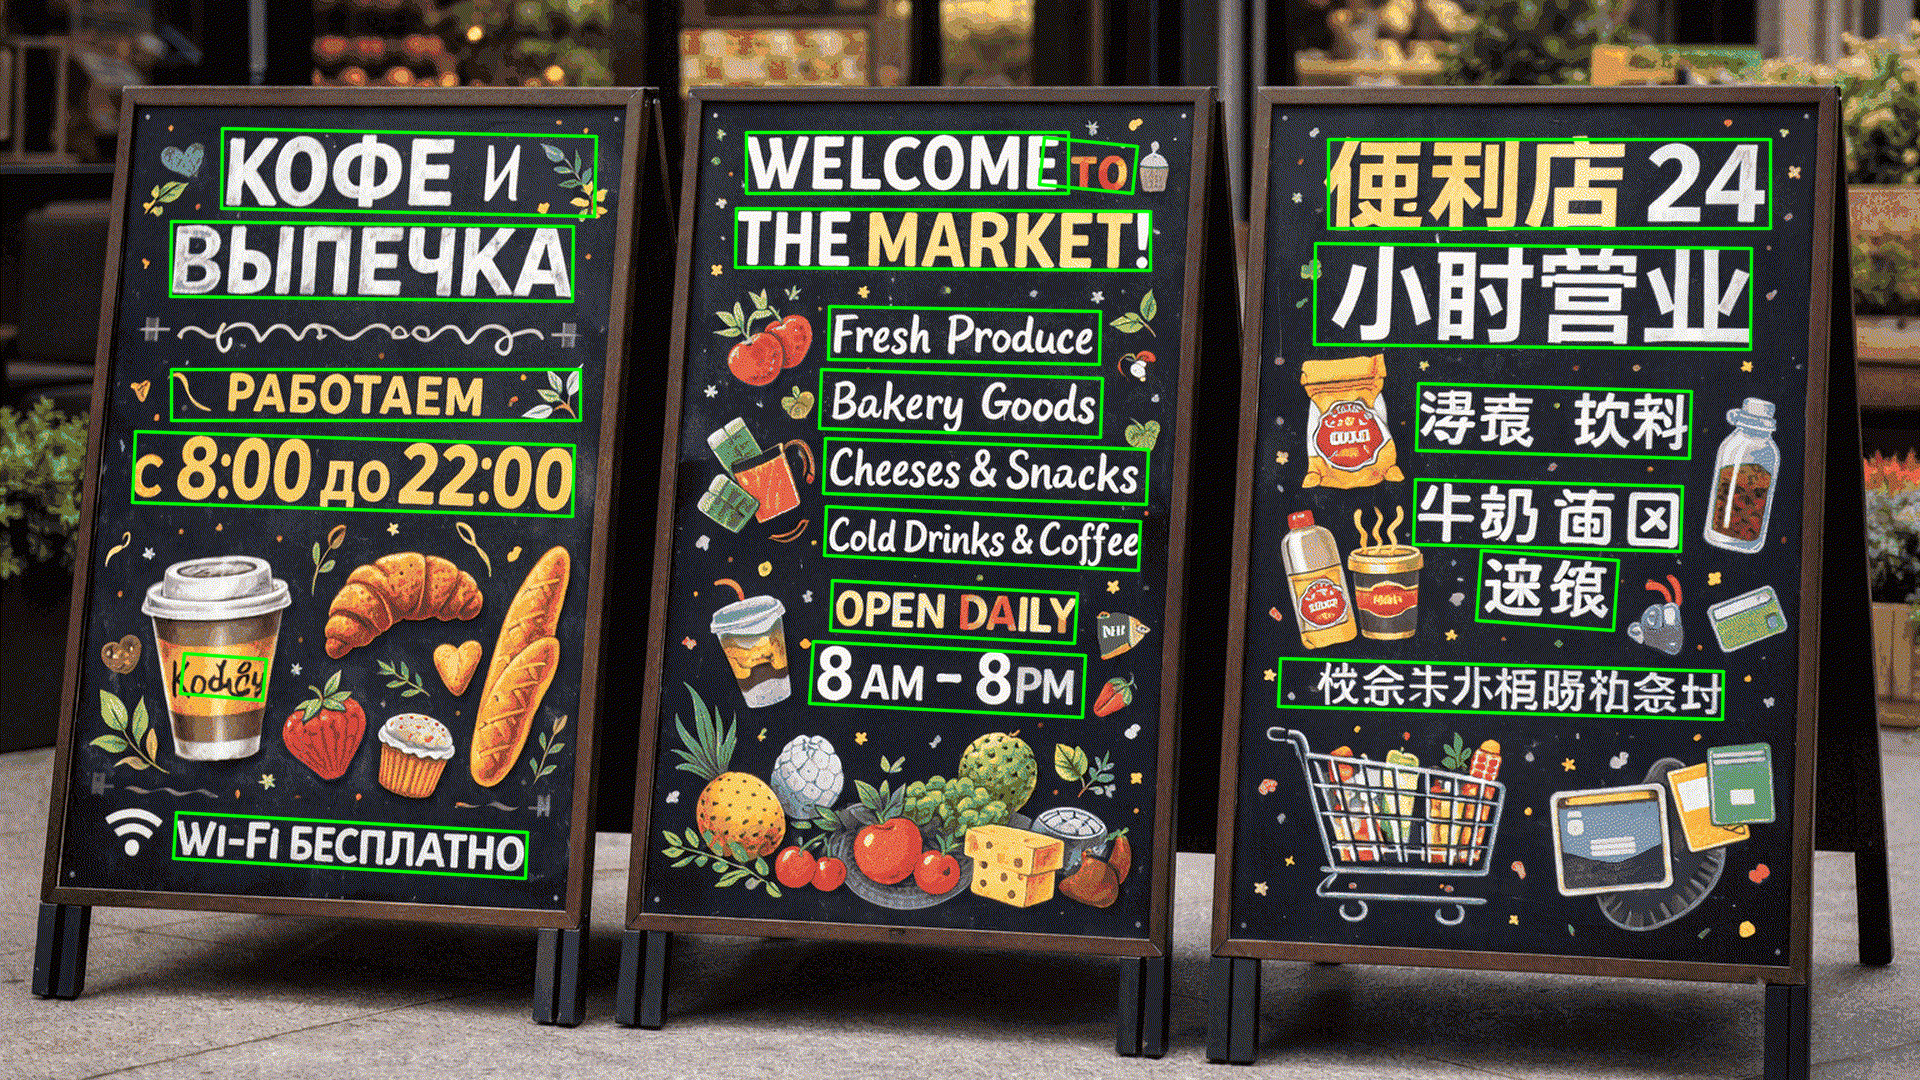
\includegraphics[width=\linewidth]{appendix/detection/single_text.png}
    \caption{Single-shot}
  \end{subfigure}\hfill
  \begin{subfigure}{0.48\linewidth}
    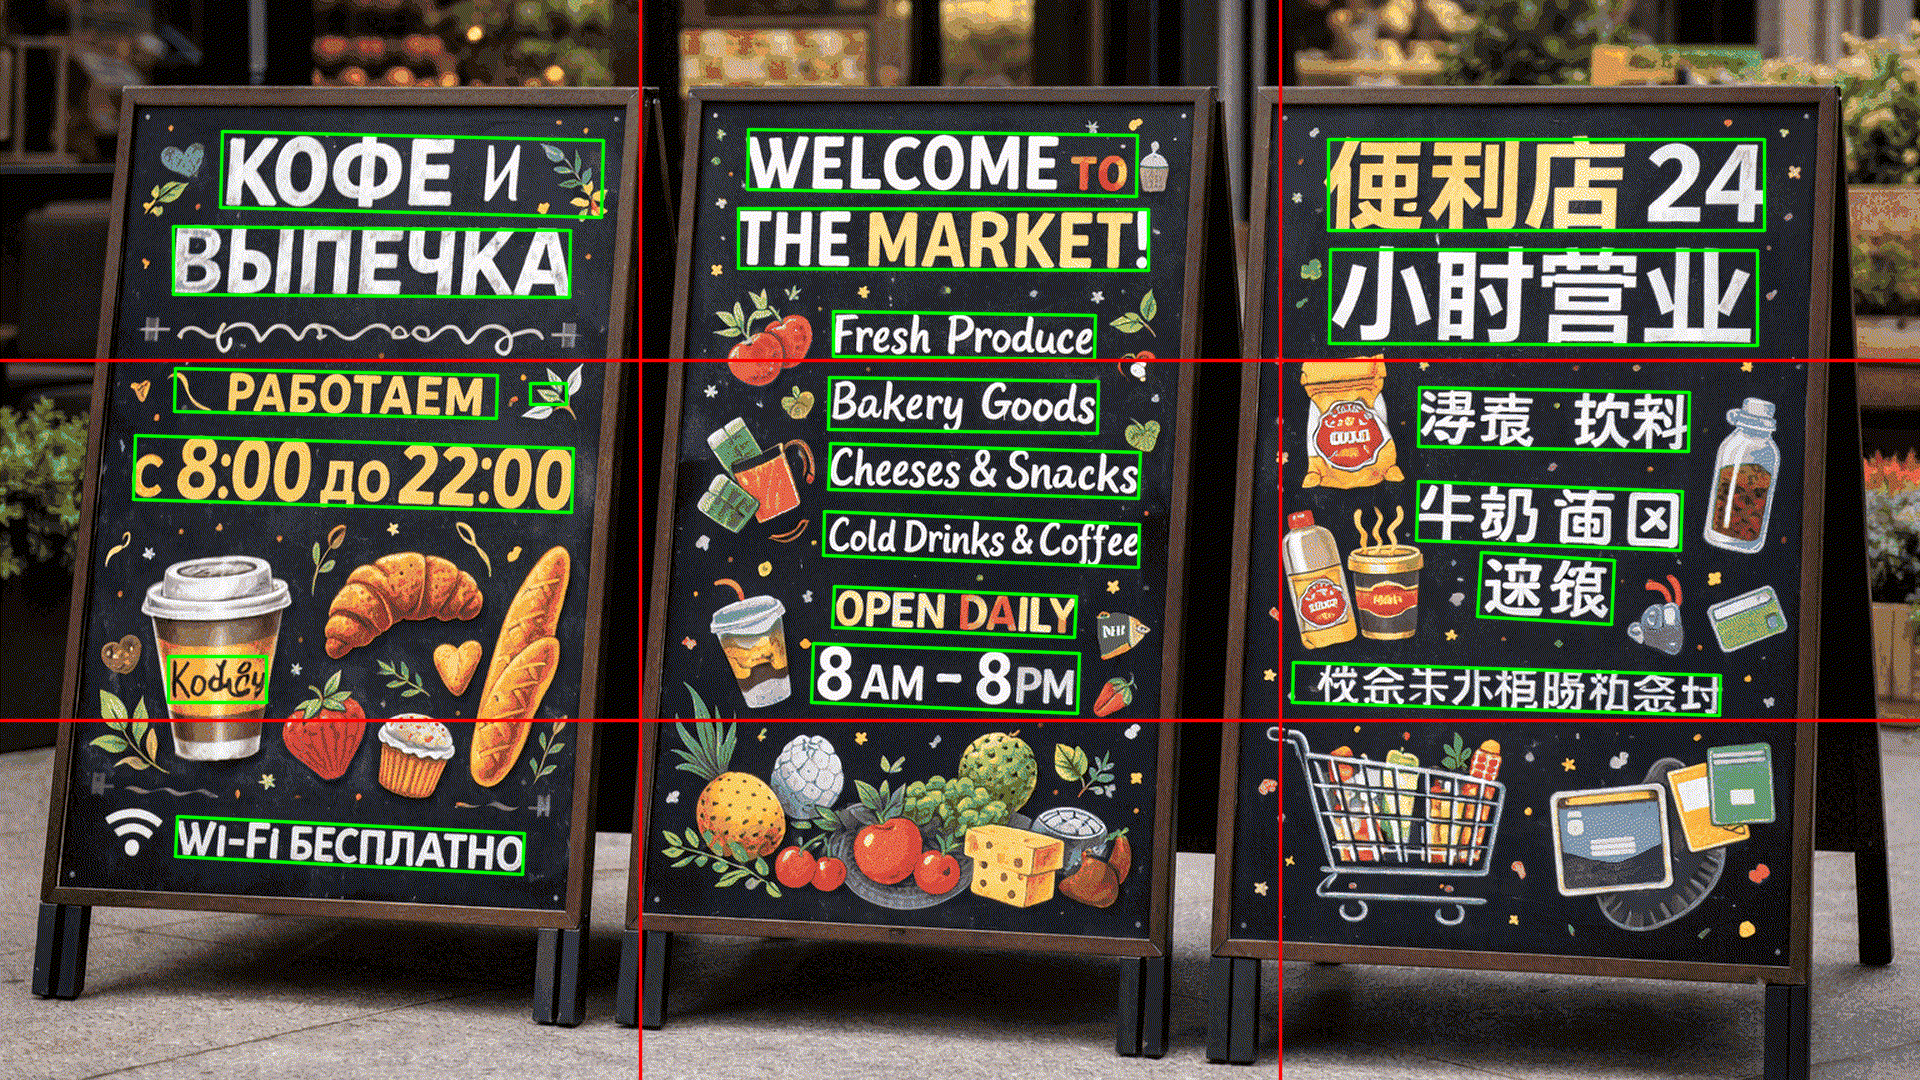
\includegraphics[width=\linewidth]{appendix/detection/tiled_text.png}
    \caption{Tiled}
  \end{subfigure}
  \caption{Визуальное сравнение режимов детекции текстовых ROI.}
  \label{fig:appendix_text_detection_modes}
\end{figure}

Рисунок~\ref{fig:appendix_text_detection_modes} показывает, что для текста tiled-режим меняет
геометрию найденных областей и может лучше покрывать мелкие надписи, но требует контроля дублей
на границах плиток.

\begin{figure}[!htbp]
  \centering
  \begin{subfigure}{0.48\linewidth}
    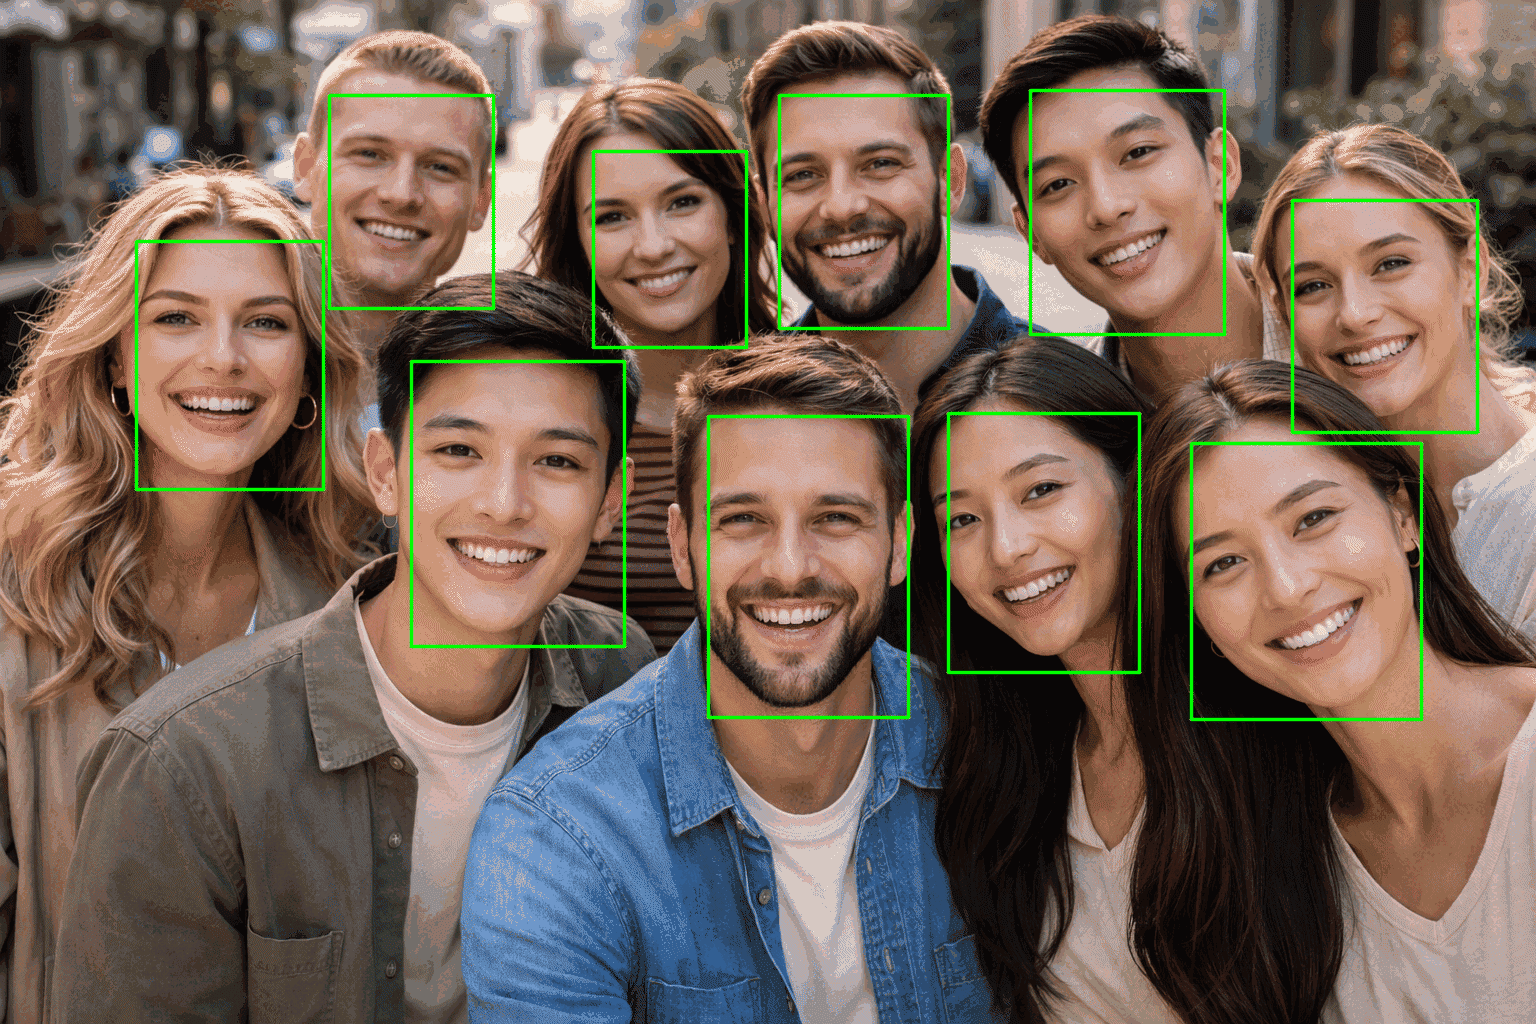
\includegraphics[width=\linewidth]{appendix/detection/single_face.png}
    \caption{Single-shot}
  \end{subfigure}\hfill
  \begin{subfigure}{0.48\linewidth}
    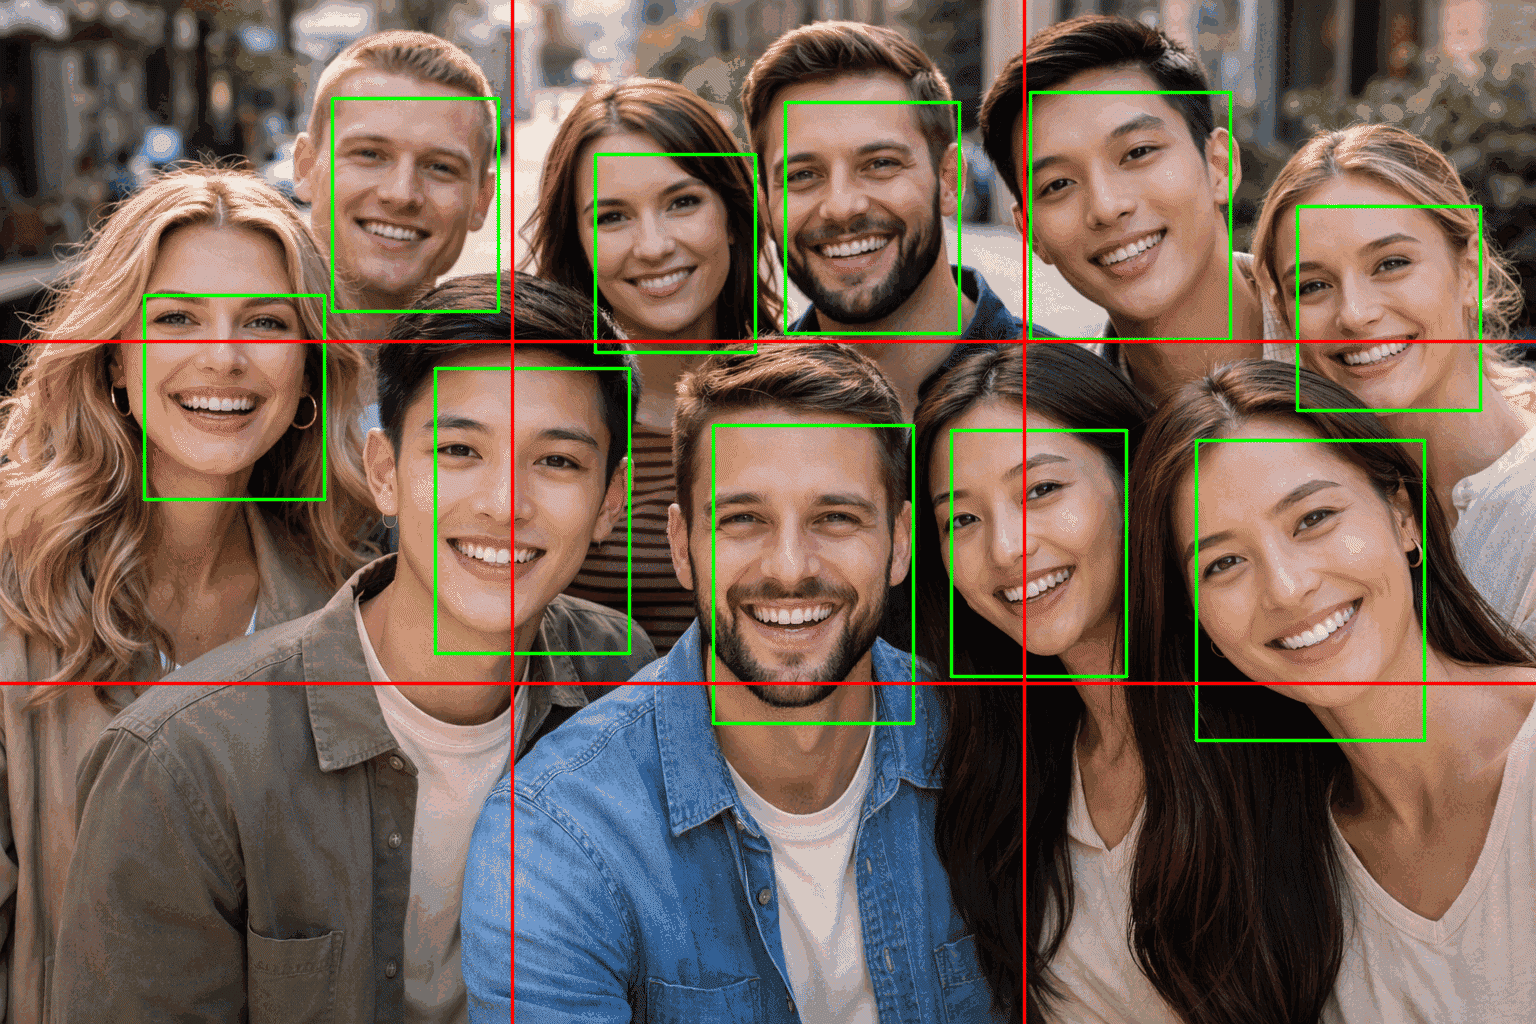
\includegraphics[width=\linewidth]{appendix/detection/tiled_face.png}
    \caption{Tiled}
  \end{subfigure}
  \caption{Визуальное сравнение режимов детекции лицевых ROI.}
  \label{fig:appendix_face_detection_modes}
\end{figure}

Рисунок~\ref{fig:appendix_face_detection_modes} показывает, что для лиц tiled-режим повышает
чувствительность к отдельным лицам в группе, но одновременно может давать более дробную
геометрию, которую нужно стабилизировать.

\begin{figure}[!htbp]
  \centering
  \begin{subfigure}{0.48\linewidth}
    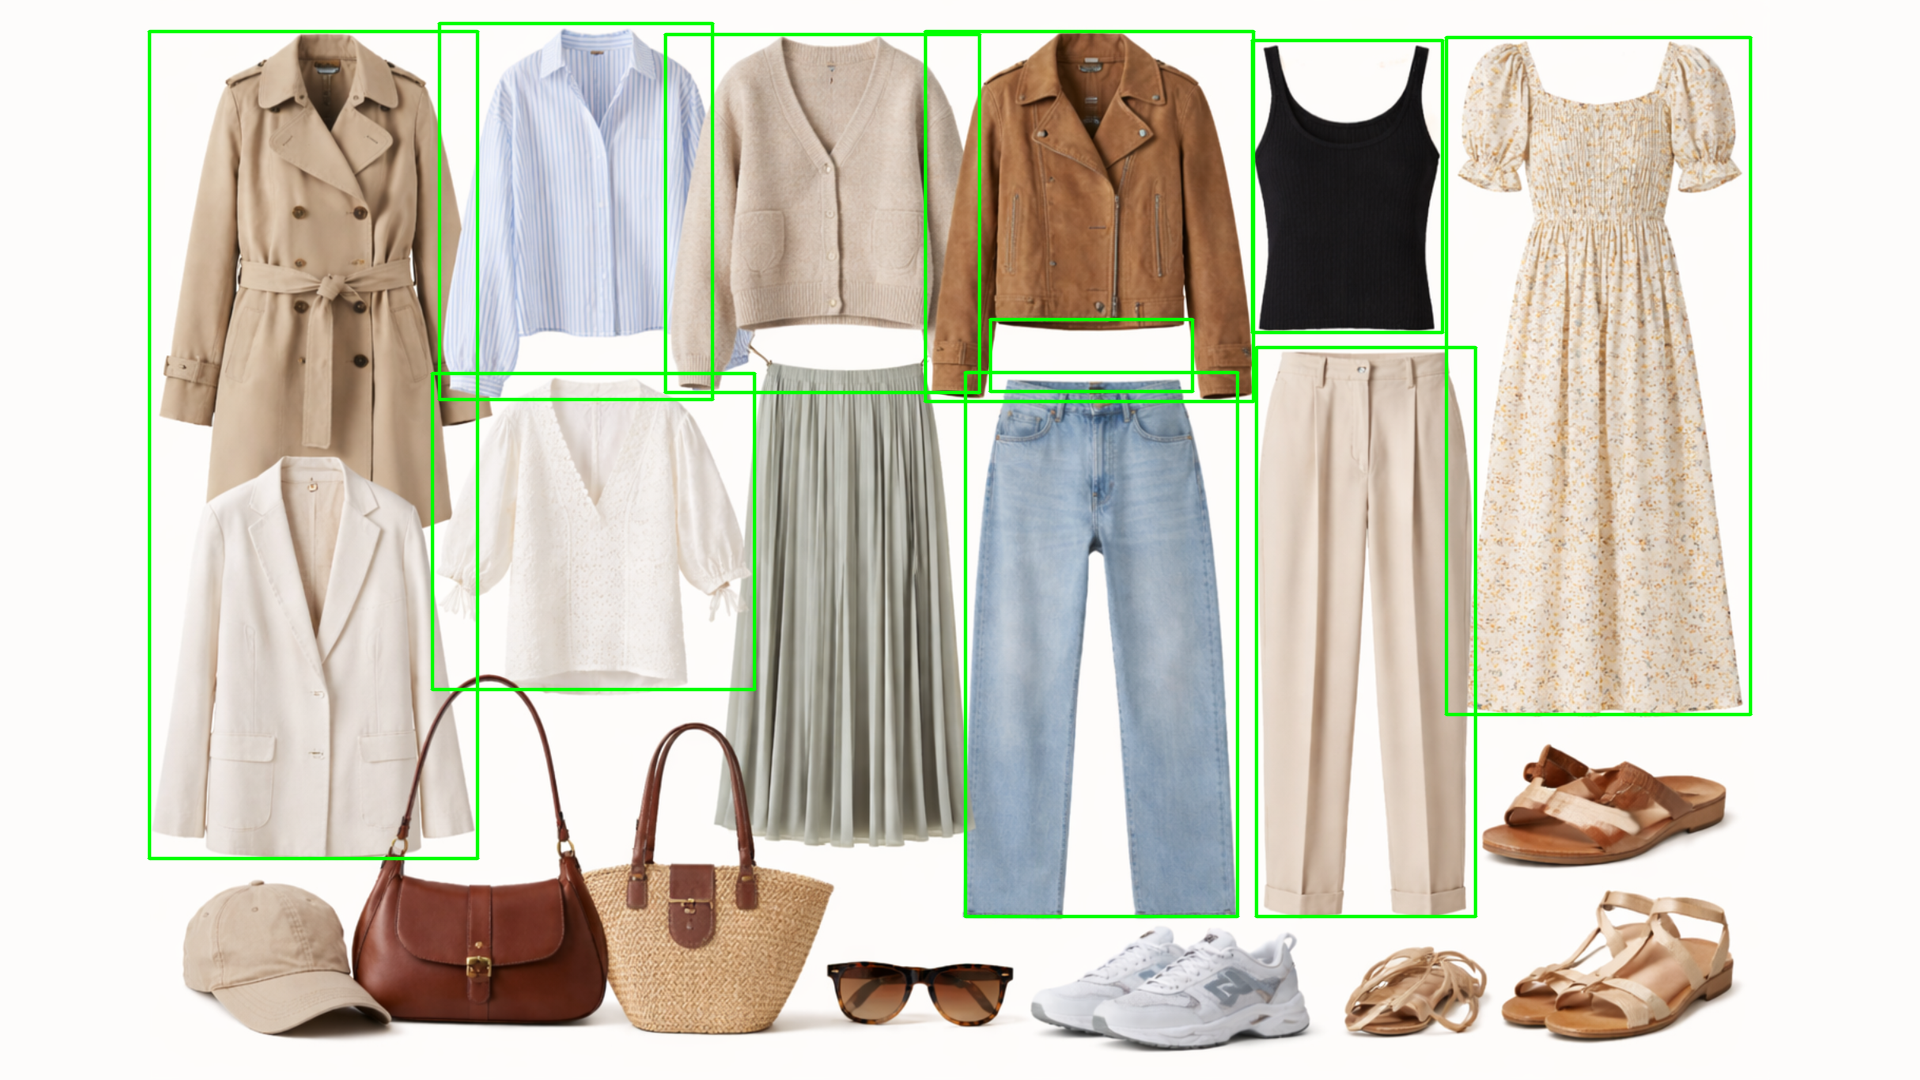
\includegraphics[width=\linewidth]{appendix/detection/single_cloth.png}
    \caption{Single-shot}
  \end{subfigure}\hfill
  \begin{subfigure}{0.48\linewidth}
    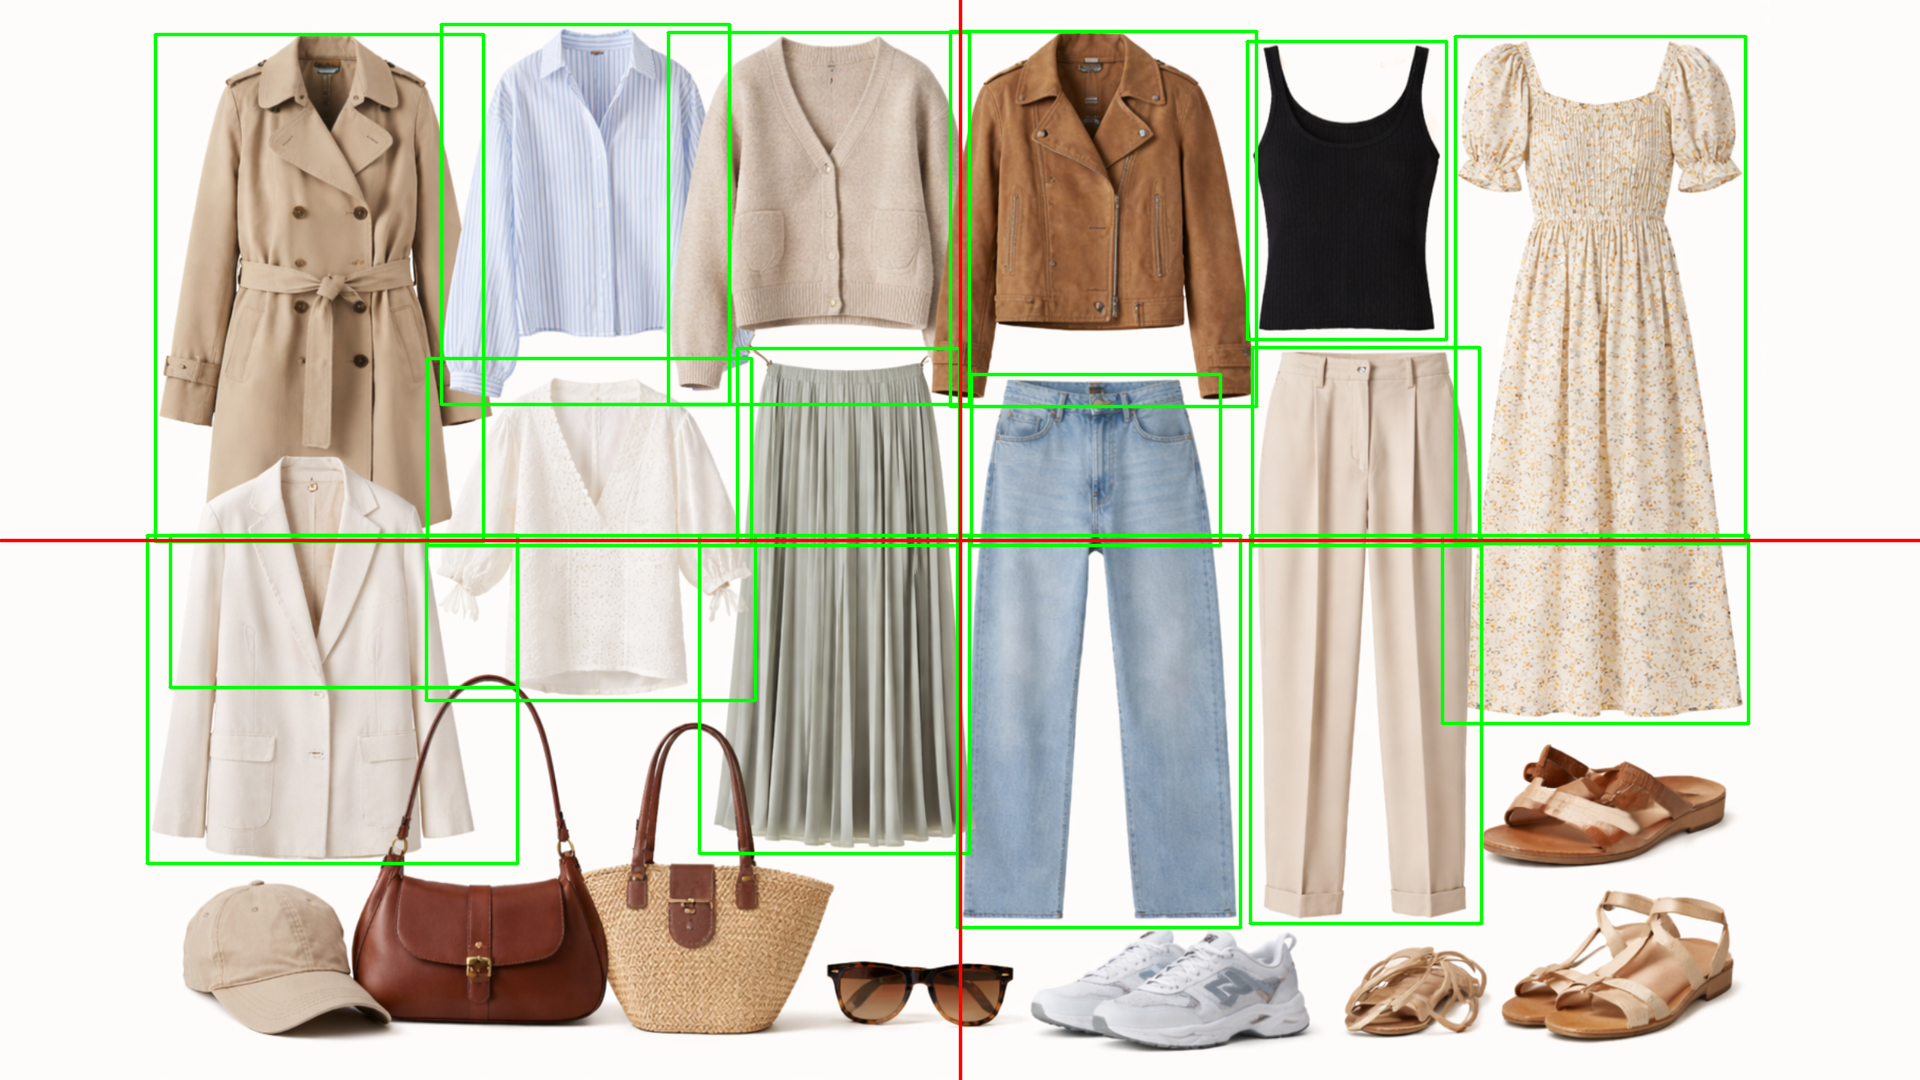
\includegraphics[width=\linewidth]{appendix/detection/tiled_cloth.png}
    \caption{Tiled}
  \end{subfigure}
  \caption{Визуальное сравнение режимов детекции текстурированных ROI.}
  \label{fig:appendix_textured_detection_modes}
\end{figure}

Рисунок~\ref{fig:appendix_textured_detection_modes} показывает, что для textured ROI tiled-режим
может изменить и число найденных областей, и их границы. В одних случаях разбиение кадра
помогает лучше локализовать мелкие или удаленные объекты, в других --- приводит к дроблению ROI
или появлению дополнительных кандидатов на границах плиток. Поэтому в IDet tiled-инференс
рассматривается как параметризуемый runtime-режим, который требует подбора под конкретную модель
и задачу. Финальная конфигурация не должна выбираться только по визуальному впечатлению:
визуальное сравнение дополняет, но не
заменяет area-based метрики и latency benchmark.

\end{document}
